\documentclass[a4paper]{book}
\usepackage[czech]{babel}
\usepackage[IL2]{fontenc}
\usepackage[utf8]{inputenc}
\usepackage{pstricks}
\usepackage{amsmath}
\usepackage{graphicx}
\usepackage{pdfpages}
\usepackage{mathrsfs}

\usepackage{fancyhdr}
\pagestyle{fancy}
\fancyhead{}
\fancyhead[LE,RO]{\thepage}
\fancyhead[RE]{\leftmark}
\fancyhead[LO]{\rightmark}

%\includeonly{wool_chap1}

\setlength{\unitlength}{1.0mm}
\sloppy

\begin{document}

\newtheorem{definition}{Definice}[chapter]
\newtheorem{theorem}{Věta}[chapter]
\newtheorem{proof}{Důkaz}[chapter]
\newtheorem{example}{Příklad}[chapter]
\newtheorem{corollary}{Tvrzení}[chapter]
\newtheorem{assumption}{Předpoklad}[chapter]

\hyphenation{prav-dě-po-dob-nost prav-dě-po-dob-nost-ní} 

\title{Úvod do ekonometrie, 4.vydání}
\author{Jeffrey M. Wooldridge}
\date{2009}
\maketitle

\tableofcontents

\chapter{Podstata ekonometrie a ekonomických dat}

\section{Empirická analýza}

Empirická analýza využívá data k testování ekonomických teorií nebo k odhadu vztahů mezi ekonomickými 
veličinami. Samotné empirické analýze dat zpravidla předchází konstrukce formálního ekonomického 
modelu. Po té, co specifikujeme ekonomický model, je třeba ho transformovat v tzv. ekonometrický model, který má 
podobu rovnice
\begin{equation}
y_i = \beta_0 + \beta_1 x_{1i} + \beta_2 x_{2i} + ... + \beta_j x_{ji} + u_i.
\end{equation}
Parametry ekonometrického modelu jsou pomocí ekonometrických metod odhadnuty na základě podkladových dat. 
Následně je možné s pomocí ekonometrického modelu formulovat a testovat nejrůznější hypotézy.

\section{Struktura ekonomických data}

\subsection{Průřezová data (cross-sectional data)}
Průřezová data jsou data týkající se vzorku náhodně vybraného z tzv. podkladové populace, která se vztahují k 
jednomu konkrétnímu časovému okamžiku. Příkladem může být příjem jednoho tisíce 
zaměstnanců na základě daňového přiznání podaného za rok 2017.

\subsection{Časové řady}
Časové řady lze charakterizovat jako soubor pozorování týkajících se jedné nebo skupiny proměnných, které 
pokrývají určitou časovou periodu. Klasickým příkladem je vývoj reálného HDP České republiky v 
průběhu let 1993 až 2017.

\subsection{Sdružená průřezová data (pooled cross sections data)}
Sdružená průřezová data jsou syntézí průřezových dat a časových řad. Příkladem tohoto typu dat může 
být příjem dvou náhodně vybraných skupin zaměstnanců za rok 2016 a 2017, kdy jsme tyto dva na sobě 
nezávislé výběry sloučili s cílem zvětšit velikost pozorovaného vzorku popř. s cílem analyzovat vývoj průměrné mzdy v čase.

\subsection{Panelová data}
Panelová data se skládají z časových řad pro každý prvek z určitého datového setu. Příkladem panelových dat je 
vývoj příjmu konkrétních domáctností v letech 2007 až 2017. Na rozdíl od sdružených průřezových 
dat se tedy struktura náhodného vzorku v čase nemění.

\chapter{Jednoduchý regresní model}

\section{Definice regresního modelu}

Jednoduchý regresní model populace je definován rovnicí
\begin{equation}
y = \beta_0 + \beta_1 x + u,
\end{equation}
kde $y$ představuje závislou (vysvětlovanou) veličinu, $x$ nezávislou (vysvětlující) veličinu a $u$ je tzv. 
chybová složka reprezentující faktory, které nejsou zahrnuty v $x$ a které mající vliv na $y$. Parametr $\beta_0$ nazýváme 
průsečíkem regresního modelu a parametr $\beta_1$ je pak sklonem regresního modelu vzhledem k nezávislé veličině $x$. Jestliže jsou ostatní faktory 
reprezentované členem $u$ konstantní, tj. $\Delta u = 0$, pak je vztah mezi $x$ a $y$ lineární.
\begin{equation}
\Delta y = \beta_1 \Delta x
\end{equation}
(2.2) implicitně předpokládá, že $E[u] = 0$. Tento předpoklad však ve skutečnosti není 
omezující, protože je vždy možné upravit parametr $\beta_0$ tak, aby $E[u] = 0$. Zásadnějším předpokladem 
je $E[u|x] = E[u] = 0$, tj. předpoklad, že chyba $u$ a vysvětlující veličina $x$ jsou nezávislé. Rovnice $E[u|x] = 0$ říká, že 
průměrná hodnota chyby $u$ je nulová napříč všemi podvýběry definovanými konkrétní hodnotou vysvětlující veličiny
$x$\footnote{Uvažujme ekonometrický model, kde $y$ představuje výnos na hektar, $x$ kvalitu půdy a $u$ zahrnuje 
množství hnojiv, které jsme použili. Pokud bude množství hnojiv nezávislé na kvalitě půdy, pak je předpoklad 
$E[u|x] = E[x] = 0$ splněn. Pokud však použijeme více hnojiva na méně kvalitní půdu, je tento předpoklad porušen.}.

Očekávaná hodnota (2.1) je daná tzv. populační regresní funkcí (population regression function - PRF)
\begin{equation}
E[y|x] = \beta_0 + \beta_1 x,
\end{equation}
kde pravděpodobnostní rozdělení veličiny $y$ je centrováno na $E[y|x]$ pro libovolnou hodnotu $x$. Situace je 
ilustrována následujícím obrázkem.

\begin{figure}[htp]
\centering
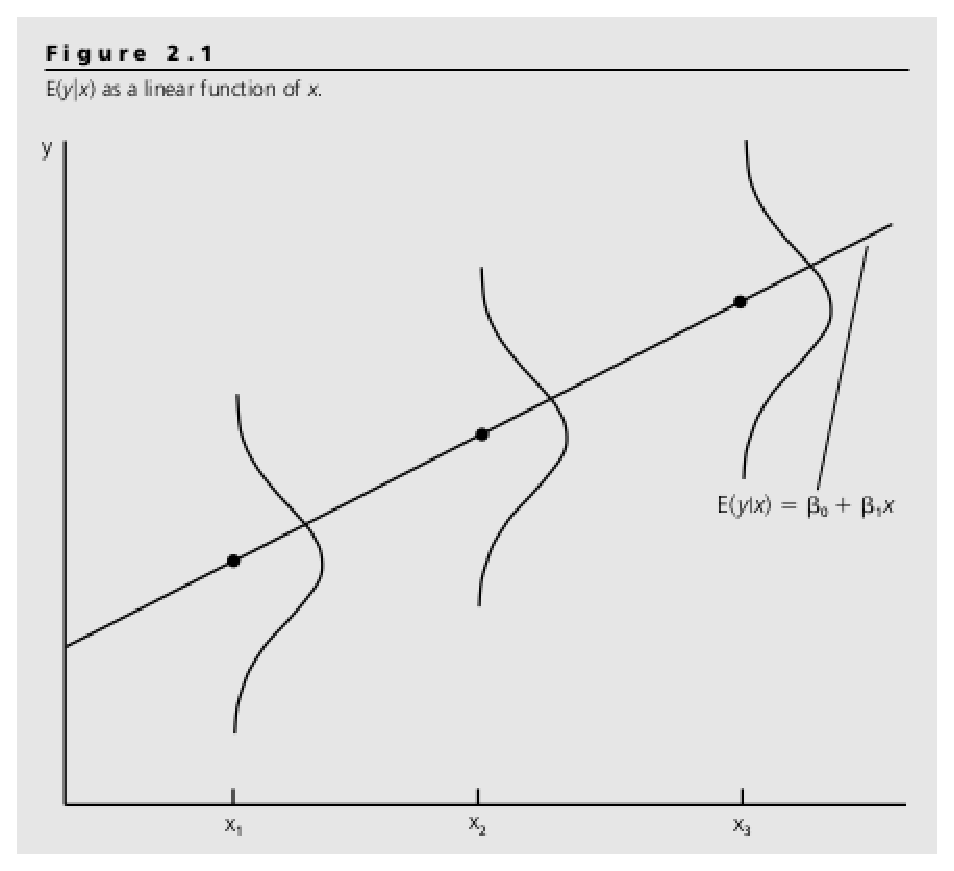
\includegraphics[scale = 0.5]{pictures/figure_2_1.eps}
\caption{$E[y|x]$ jako lineární funkce $x$}
\label{figure_2_1}
\end{figure} 

S ohledem na $E[u|x] = 0$ je užitečné (2.1) rozdělit na dvě části. Část $\beta_0 + \beta_1 x$ reprezentující $E[y|x]$ je nazývána systematickou částí $y$, tj. částí vysvětlenou nezávislou proměnnou $x$; část $u$ je 
nazývána nesystematickou částí, tj. částí $y$, která není vysvětlená nezávislou proměnnou $x$.

\section{Metoda nejmenších čtverců}

Uvažujme jednoduchý regresní model
\begin{equation}
y_i = \beta_0 + \beta_1 x_i + u_i.
\end{equation}
Protože $E[u|x] = E[u] = 0$ implikuje nezávislost $x$ a $u$, platí
\begin{equation}
cov(x,u) = E[ux] - E[x]E[y] = E[ux] = 0.
\end{equation}
Rovnice $E[u] = 0$ a $E[xy] = 0$ lze přepsat do tvaru
\begin{equation}
E[y - \beta_0 - \beta_1 x] = 0
\end{equation}
a
\begin{equation}
E[x(y - \beta_0 - \beta_1 x)] = 0.
\end{equation}
Odhady parametrů $\hat{\beta}_0$ a $\hat{\beta}_1$ jsou řešením soustavy rovnic
\begin{equation}
n^{-1} \sum_{i = 1}^n (y_i - \hat{\beta}_0 - \hat{\beta}_1x_i) = 0
\end{equation}
a
\begin{equation}
n^{-1} \sum_{i = 1}^n x_i (y_i - \hat{\beta}_0 - \hat{\beta}_1x_i) = 0.
\end{equation}
Protože $\bar{y} = \hat{\beta}_0 + \hat{\beta}_1 \bar{x}$, tj.
\begin{equation}
\hat{\beta}_0 = \bar{y} - \hat{\beta}_1 \bar{x},
\end{equation}
lze rovnici (2.9) postupně upravit následujícím způsobem.
\begin{equation}
\sum_{i = 1}^n x_i(y_i - (\bar{y} - \hat{\beta}_1 \bar{x}) - \hat{\beta}_1x_i) = 0
\end{equation}
\begin{equation}
\sum_{i = 1}^n x_i(y_i - \bar{y}) = \hat{\beta}_1 \sum_{i = 1}^n x_i(x_i - \hat{x})
\end{equation}
S využitím vztahů
\begin{equation}
\sum_{i = 1}^n x_i (x_i - \bar{x}) = \sum_{i = 1}^n (x_i - \bar{x})^2
\end{equation}
a
\begin{equation}
\sum_{i = 1}^n x_i(y_i - \bar{y}) = \sum_{i = 1}^n (x_i - \bar{x})(y_i - \bar{y})
\end{equation}
lze $\hat{\beta}_1$ vyjádřit jako
\begin{equation}
\hat{\beta}_1 = \frac{\sum_{i = 1}^n (x_i - \bar{x})(y_i - \bar{y})}{\sum_{i = 1}^n (x_i - \bar{x})^2},
\end{equation}
Pokud čitatel i jmenovatel (2.15) vydělíme $n - 1$, lze odhad $\hat{\beta}_1$ interpretovat jako podíl kovariance mezi $x$ a $y$ a výběrového rozptylu $x$. Odhady (2.10) a (2.15) se nazývají odhady nejmenších čtverců 
(ordinary least square estimates - OLS estimates).

Rovnici hodnot odhadnutých na základě regresního modelu, označovanou jako OLS regresní přímka popř. jako 
výběrovou regresní funkci (sample regression function - SRF), zapisujeme ve tvaru
\begin{equation}
\hat{y}_i = \hat{\beta}_0 + \hat{\beta}_ix_1
\end{equation}
a rovnici reziduí jednotlivých pozorování\footnote{Člen $u$ populačního regresního modelu $y = \beta_0 + 
\beta_1 x + u$ označujeme jako chybu. Člen $\hat{u}$ odhadu populačního regresního modelu $y = \hat{\beta}_0 + 
\hat{\beta}_1 x + \hat{u}$ pak označujeme jako reziduum.} pak jako
\begin{equation}
\hat{u}_i = y_i - \hat{y}_i = y_i - \hat{\beta}_0 - \hat{\beta}_1x_i.
\end{equation}
Jestliže parciální derivace součtu čtverců reziduí
\begin{equation}
\sum_{i = 1}^n \hat{u}_i^2 = \sum_{i = 1}^n (y_i - \hat{\beta}_0 - \hat{\beta}_1 x_1)^2
\end{equation}
dle $\hat{\beta}_0$ a $\hat{\beta}_1$ položíme rovny nule a řešíme pro $\hat{\beta}_0$ a $\hat{\beta}_1$, 
získáme (2.10) a (2.15). Jinými slovy (2.10) a (2.15) minimalizují (2.18) - odtud pojem metoda nejmenších čtverců.

\section{Vlastnosti OLS pro náhodný výběr}

Následující tvrzení implicitně předpokládají, že odhad regresního modelu je proveden na náhodném výběru z populace, kterou zamýšlíme 
tímto modelem popsat.

\subsection{Algebraické vlastnosti OLS}

Průměr reziduí $\hat{u}_i = y_i - \hat{\beta}_0 - \hat{\beta}_1x_1$ je roven nule, tj.
\begin{equation}
\sum_{i = 1}^n \hat{u}_i = 0.
\end{equation}
Toto tvrzení je přímým důsledkem toho, jakým způsobem jsou zkonstruovány odhady $\hat{\beta}_0$ a 
$\hat{\beta}_1$.

Vztah (2.19) implikuje nulovou OLS kovarianci, tj.
\begin{equation}
\sum_{i = 1}^n x_i \hat{u}_i = 0.
\end{equation}

Bod $(\bar{x}, \bar{y})$ se vždy nachází na OLS regresní přímce. Toto tvrzení vyplývá z (2.10).

Na OLS lze pohlížet jako na metodu, která rozdělí pozorování $y_i$ na $\hat{y}_i = \hat{\beta}_0 + 
\hat{\beta}_1x_1$ predikované OLS přímkou a rezidua $\hat{u}_i = y_i - \hat{y}_i$. Rezidua $\hat{u}_i$ a 
predikované hodnoty $\hat{y}_i$ jsou v rámci náhodného výběru nekorelované.

Definujme celkový součet čtverců (total sum of squares - SST), vysvětlený součet čtverců (explained sum of 
squares - SSE) a reziduální součet čtverců (residual sum of squares - SSR) jako
\begin{equation}
SST \equiv \sum_{i = 1}^n (y_i - \bar{y})^2,
\end{equation}
\begin{equation}
SSE \equiv \sum_{i = 1}^n (\hat{y}_i - \bar{y})^2,
\end{equation}
a
\begin{equation}
SSR \equiv \sum_{i = 1}^n \hat{u}_i^2.
\end{equation}
Platí
\begin{equation}
SST = SSE + SSR.
\end{equation}
To lze dokázat následujícím způsobem s využitím $\sum_{i = 1}^n \hat{u}_i(\hat{y}_i - \bar{y}) = 0$, což je 
ekvivalentní předpokladu nulové výběrové kovariance mezi rezidui $\hat{u}_i$ a predikovanými hodnotami $\hat{y}_i$.
\begin{equation}
\begin{split}
SST = \sum_{i = 1}^n (y_i - \bar{y})^2 & = \sum_{i = 1}^n [(y_i - \hat{y}_i) + (\hat{y}_i + \bar{y})]^2\\
& = \sum_{i = 1}^n [\hat{u}_i + (\hat{y}_i - \bar{y})]^2\\
& = \sum_{i = 1}^n \hat{u}_i^2 + 2 \sum_{i = 1}^n \hat{u}_i(\hat{y}_i - \bar{y}) + \sum_{i = 1}^n (\hat{y}_i - 
\bar{y})^2\\
& = SSR + SSE
\end{split}
\end{equation}

\subsection{Míra shody (goodness-of-fit)}

Pro vyjádření míry shody mezi pozorovanými a predikovanými hodnotami se v ekonometrii používá tzv. $R^2$, 
někdy též nazývaný koeficient determinace.
\begin{equation}
R^2 = \frac{SSE}{SST} = 1 - \frac{SSR}{SST}.
\end{equation}
Z výše uvedené rovnice vyplývá, že $R^2$ je poměrem mezi vysvětleným a celkovým rozptylem závislé proměnné. 
$R^2$ tak vždy nabývá hodnoty v rozmezí nula až jedna. V případě jednoduchého regresního modelu s jednou 
nezávislou proměnnou je $R^2$ rovno druhé mocnině korelačního koeficientu mezi $y_i$ a $\hat{y}_i$; odtud 
pochází název $R^2$.

V sociálních vědách se velmi často setkáváme s regresními modely, jejichž $R^2$ je poměrně nízké. Zdánlivě 
nízké $R^2$ nemusí nezbytně znamenat, že model je špatný. Takovýto model může stále dobře popisovat 
lineární vztahy mezi vybranými veličinami. Problémem modelu však je, že nezávislá veličina $x$ podchycuje 
pouze menší část variace závislé veličiny $y$.

\section{Měrné jednotky a nelinearity v regresním modelu}

\subsection{Efekt změny měrné jednotky na OLS statistiky}

Jestliže změníme měrné jednotky závislé či nezávislé proměnné, změní se OLS odhady deterministickým způsobem.

Pokud je závislá proměnná $y$ vynásobena konstantou $c$, pak jsou OLS odhady průsečíku $\hat{\beta}_0$ a sklonu 
regresního modelu $\hat{\beta}_1$ taktéž vynásobeny konstantou $c$.

V případě, že je nezávislá veličina $x$ vydělená popř. vynásobena nenulovou konstantou $c$, je odhad sklon 
$\hat{\beta_1}$ této nezávislé veličiny taktéž vynásoben popř. vydělen touto konstantou. Odhad průsečíku $\hat{\beta}_0$ regresního modelu zůstává nezměněn.

Míra shody vyjádřená pomocí $R^2$ je změnou měrné jednotky nedotčena.

\subsection{Zahrnutí nelinearit do regresního modelu}

\subsubsection{Log-level regresní model}

Jednoduchý regresní model $y = \beta_0 + \beta_1 x + u$ označujeme jako level-level model. Jeho 
triviální modifikací je tzv. log-level model
\begin{equation}
ln(y) = \beta_0 + \beta_1 x + u.
\end{equation}
Tento model říká, o kolik procentních bodů se zvýší $y$, jestliže se $x$ zvýší o jednu jednotku. Jinými slovy
\begin{equation}
\%\Delta y \approx (100 \beta_1) \Delta x.
\end{equation}
Veličina $100 \beta_1$ je někdy nazývána semi-elasticitou. Model (2.27) lze upravit do tvaru
\begin{equation}
y = e^{\beta_0 + \beta_1 x + u},
\end{equation}
Takto upravený model je typický exponenciálním průběhem.

\begin{figure}[htp]
\centering
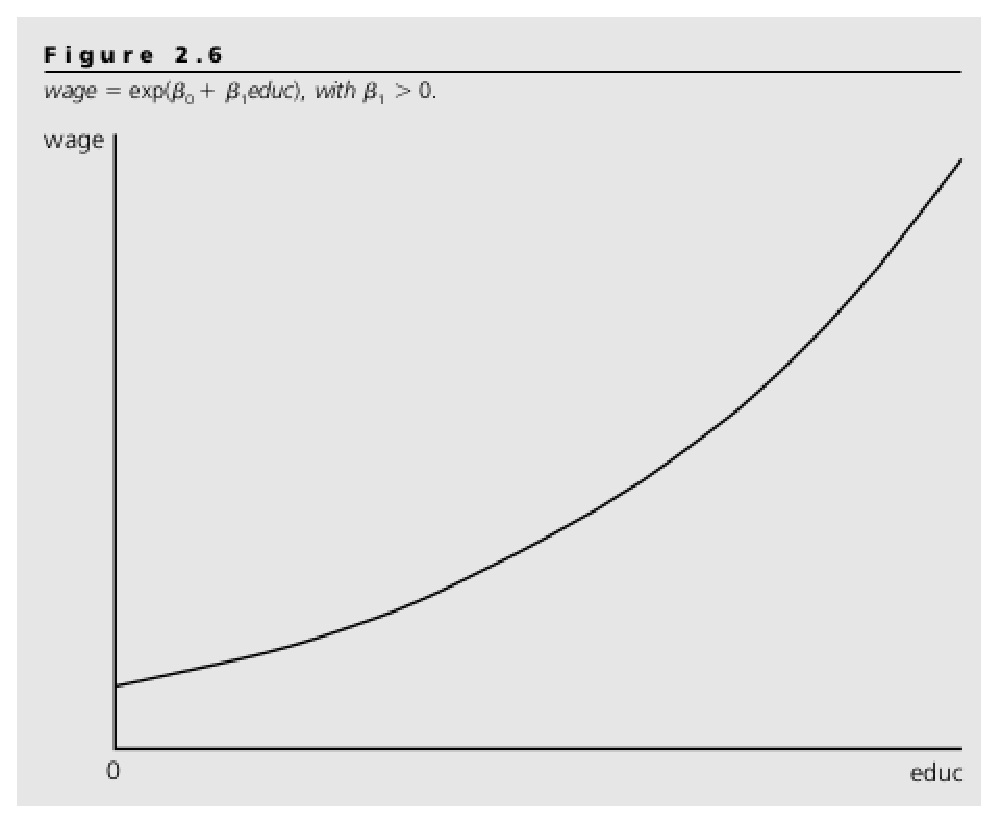
\includegraphics[scale = 0.5]{pictures/figure_2_6.eps}
\caption{Regresní model s exponenciálním průběhem}
\label{figure_2_6}
\end{figure} 

\subsubsection{Log-log regresní model}

Další modifikací základního regresního modelu je tzv. log-log model nazývaný též modelem konstantní elasticity, který má tvar
\begin{equation}
ln(y) = \beta_0 + \beta_1 ln(x) + u.
\end{equation}
Tento model říká, že pokud se $x$ zvýší o 1\%, zvýší se $y$ o $\beta_1$\%, což je obvyklá interpretace elasticity.

\subsubsection{Změna měrné jednotky}

Pokud ve výše uvedených modelech závislou popř. nezávislou proměnnou vynásobíme konstantou $c$, sklon regresního modelu zůstane 
nezměněn, nicméně jeho průsečík se změní na $ln(c) + \beta_0$.

\subsection{Význam pojmu lineární regrese}

Pojem lineární regrese se váže k parametrům modelu, nikoliv k podkladovým datům. Model
\begin{equation}
y = \beta_0 + \beta_1 x^2 + u
\end{equation}
je tak stále lineárním regresním modelem, nicméně model
\begin{equation}
y = \frac{1}{\beta_0 + \beta_1 x + u}
\end{equation}
již lineárním regresním modelem není.

\section{Očekávaná hodnota a rozptyl OLS odhadů}

\subsection{Nestrannost OLS odhadů (unbiasedness of OLS)}

Tuto kapitolu zahájíme souhrnem předpokladů, na základě kterých budeme následně dokazovat nestrannost OLS odhadů.

\begin{assumption}[SLR.1 - lineární model]
V populačním regresním modelu je vztah mezi závislou veličinou $y$ a nezávislou veličinou $x$ a chybou $u$ charakterizován funkcí ve tvaru
\begin{equation}
y = \beta_0 + \beta_1 x + u,
\end{equation}
kde $\beta_0$ a $\beta_1$ jsou populační průsečík a sklon.

\raggedleft{$\clubsuit$}
\end{assumption}

\begin{assumption}[SLR.2 - náhodný výběr]
Máme k dispozici náhodný výběr velikosti $n$, $\{(x_i, y_i): i = 1, 2, ..., n \}$, který sleduje populační model definovaný v předpokladu SLR.1.

\raggedleft{$\clubsuit$}
\end{assumption}

\begin{assumption}[SLR.3 - výběrový rozptyl vysvětlující veličiny]
Náhodně vybrané vysvětlující proměnné $\{x_i, i = 1, 2, ..., n\}$ nenabývají stejné hodnoty. Jinými slovy 
výběrový rozptyl vysvětlující proměnné je různý od nuly.

\raggedleft{$\clubsuit$}
\end{assumption}

\begin{assumption}[SLR.4 - nulová podmíněná hodnota]
Očekávaná hodnota chyby $u$ je pro libovolnou hodnotu závislé veličiny rovna nule, tj.
\begin{equation}
E[u|x] = 0.
\end{equation}

\raggedleft{$\clubsuit$}
\end{assumption}

Skutečný populační sklon $\beta_1$ neznáme, máme však k dispozici jeho odhad - výběrový sklon 
$\hat{\beta}_1$. Ten je náhodnou veličinou, a proto má očekávanou hodnotu a rozptyl.

Protože $\sum_{i = 1}^n (x_i - \bar{x})(y_i - \bar{y}) = \sum_{i = 1}^n (x_i - \bar{x})y_i$, lze $\hat{\beta}_1$ vyjádřit jako
\begin{equation}
\hat{\beta}_1 = \frac{\sum_{i = 1}^n (x_i - \bar{x})y_i}{\sum_{i = 1}^n (x_i - \bar{x})^2}.
\end{equation}
Vzhledem k tomu, že $SST_x = \sum_{i = 1}^n (x_i - \bar{x})^2$ a $y_i = \beta_0 + \beta_1 x_i + u_i$, můžeme výše 
uvedenou rovnici upravit do tvaru
\begin{equation}
\hat{\beta_i} = \frac{\sum_{i = 1}^n (x_i - \bar{x})(\beta_0 + \beta_1 x_i + u_i)}{SST_x}.
\end{equation}
Čitatel lze pak rozepsat na
\begin{multline}
\sum_{i = 1}^n (x_i - \bar{x})\beta_0 + \sum_{i = 1}^n (x_i - \bar{x})\beta_1 x_1 + \sum_{i = 1}^n (x_i - \bar{x}) 
u_i\\
= \beta_0 \sum_{i = 1}^n (x_i - \bar{x})  +\beta_1 \sum_{i = 1}^n (x_i - \bar{x})x_i + \sum_{i = 1}^n (x_i - \bar{x}) 
u_i.
\end{multline}
Protože $\sum_{i = 1}^n (x_i - \bar{x}) = 0$ a $\sum_{i = 1}^n (x_i - \bar{x})x_i = \sum_{i = 1}^n (x_i - \bar{x})^2 = 
SST_x$, platí
\begin{equation}
\hat{\beta}_1 = \beta_1 + \frac{\sum_{i = 1}^n (x_i - \bar{x})u_i}{SST_x} = \beta_1 + \frac{1}{SST_x}\sum_{i = 1}^n d_i 
u_i,
\end{equation}
kde $d_i = x_i - \bar{x}$. OLS odhad $\hat{\beta}_1$ je tedy roven součtu populačního sklonu $\beta_1$ a členu, který je 
lineární kombinací chyb $\{u_1, u_2, ..., u_n\}$.

\begin{theorem}[Nestrannost OLS odhadů]
Při splnění předpokladů SLR.1 až SLR.4 platí
\begin{equation}
E[\hat{\beta}_0] = \beta_0
\end{equation}
a
\begin{equation}
E[\hat{\beta}_1] = \beta_1
\end{equation}
pro libovolné hodnoty $\beta_0$ a $\beta_1$. Jinými slovy $\hat{\beta}_0$ je nestranným odhadem $\beta_0$ a 
$\hat{\beta}_1$ je nestranným odhadem $\beta_1$.

\raggedleft{$\clubsuit$}
\end{theorem}

\begin{proof}
Vzhledem k tomu, že $SST_x$ a $d_i$ jsou pouze funkcí $x_i$, je jejich podmíněná hodnota nenáhodná. Při splnění předpokladů SLR.2 až SLR.4 je očekávaná hodnota $u_i$ 
podmíněná $\{x_1, x_2, ..., x_n\}$ nulová, a tudíž
\begin{multline}
E[\hat{\beta}_1] = \beta_1 + E\left[\frac{1}{SST_x} \sum_{i = 1}^n d_i u_i \right] = \beta_1 + \frac{1}{SST_x}\sum_{i = 
1}^n E[d_i u_i]\\
= \beta_1 + \frac{1}{SST_x}\sum_{i = 1}^n d_i E[u_i] = \beta_1 + \frac{1}{SST_x}\sum_{i = 1}^n d_i \cdot 0 = \beta_1.
\end{multline}
Protože nestrannost je platná pro libovolné $\{x_1, x_2, ..., x_n\}$, je odhad $\hat{\beta}_1$ nestranný i bez podmínění na $\{x_1, x_2, ..., x_n\}$.

Důkaz nestrannosti $\hat{\beta}_0$ je triviální. Výchozím bodem je rovnice
\begin{equation}
\hat{\beta}_0 = \bar{y} - \hat{\beta}_1\bar{x} = \beta_0 + \beta_1 \bar{x} + \bar{u} - \hat{\beta}_1 \bar{x} = \beta_0 
+ (\beta_1 - \hat{\beta}_1)\bar{x} + \bar{u}.
\end{equation}
Pokud na levou i pravou stranu rovnice aplikujeme očekávanou hodnotu, získáme
\begin{equation}
E[\hat{\beta}_0] = \beta_0 + E[\beta_1 - \hat{\beta}_1\bar{x}] + E[\bar{x}] = \beta_0 + E[\beta_1 - 
\hat{\beta}_1]\bar{x} = \beta_0
\end{equation}

\raggedleft{$\clubsuit$}
\end{proof}

Je důležité zdůraznit, že pokud je některý z předpokladů SLR.1 až SLR.4 porušen, výše uvedená odvození 
neplatí a OLS odhady tím pádem nejsou nestranné.

\subsection{Rozptyl OLS odhadů}

\begin{assumption}[SLR.5 - homoskedasticita]
Chyba $u$ má konstantní rozptyl bez ohledu na hodnotu vysvětlující veličiny, tj.
\begin{equation}
var[u|x] = \sigma^2.
\end{equation}

\raggedleft{$\clubsuit$}
\end{assumption}

Homoskedasticita nehraje žádnou roli v tom, zda-li jsou odhady $\hat{\beta}_0$ a $\hat{\beta}_1$ nestranné. 
Předpoklad SLR.5 přidáváme, protože usnadňuje výpočet rozptylu $\hat{\beta}_0$ a $\hat{\beta}_1$. Soubor 
předpokladů SLR.1 až SLR.5 označujeme jako Gauss-Markovovy předpoklady.

Vzhledem k tomu, že
\begin{equation}
var[u|x] = E[u^2|x] - E[u|x]^2 = E[u^2|x] = E[u^2] = \sigma^2,
\end{equation}
je očekávaná hodnota $u^2$ rovna $\sigma^2$, nebo-li $\sigma^2 = E[u^2] = var[u]$.

Pokud $var[u]$ závisí na $x$, říkáme, že chybový člen vykazuje heteroskedasticitu.

\begin{figure}[htp]
\centering
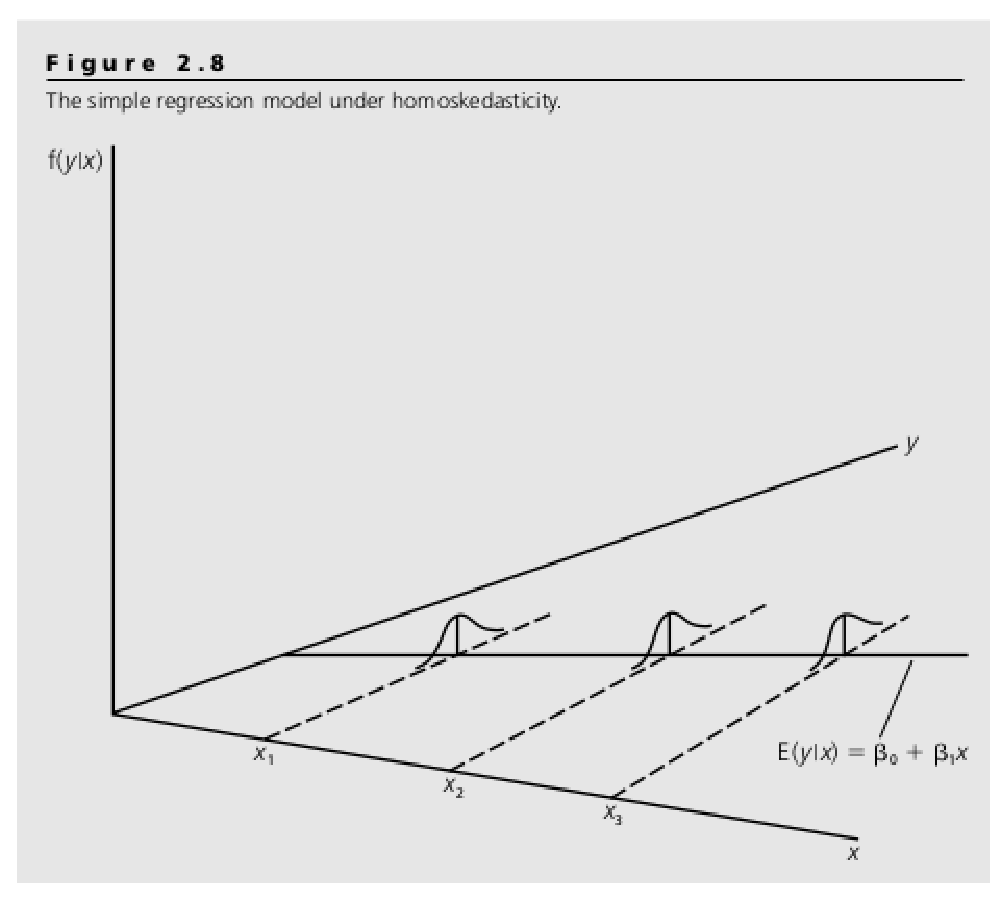
\includegraphics[scale = 0.5]{pictures/figure_2_8.eps}
\caption{Chybový člen vykazující homoskedasticitu}
\label{figure_2_6}
\end{figure} 

\begin{figure}[htp]
\centering
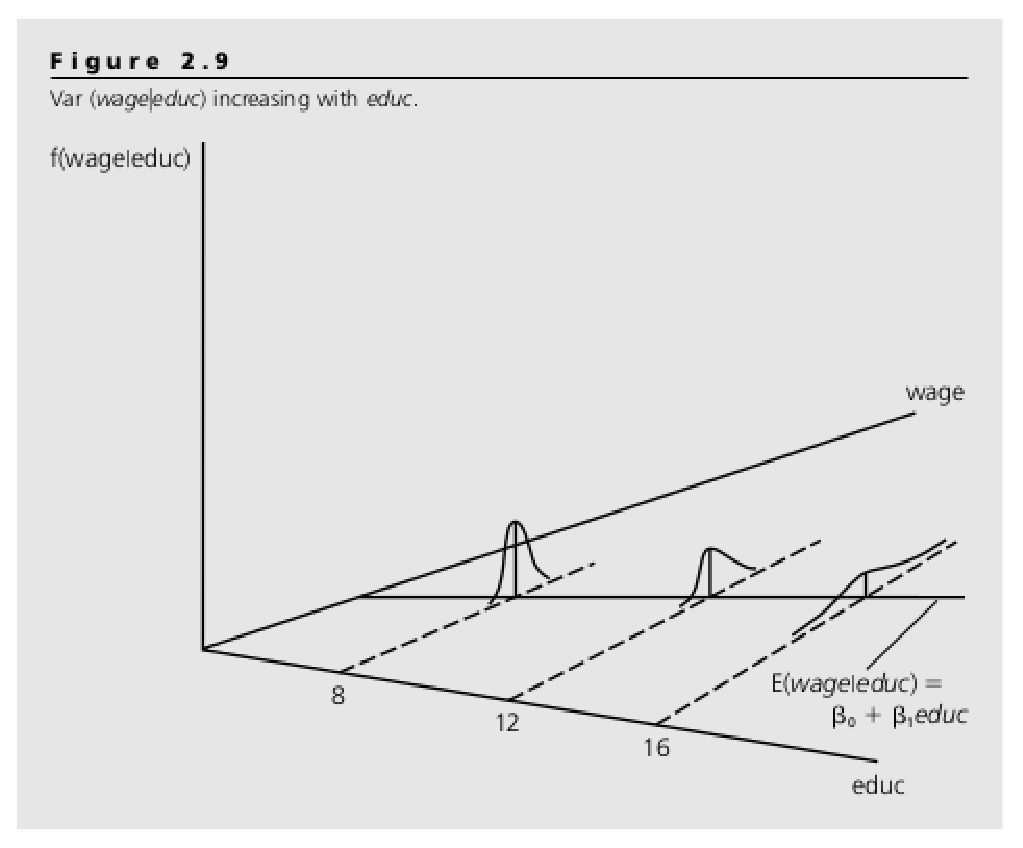
\includegraphics[scale = 0.5]{pictures/figure_2_9.eps}
\caption{Chybový člen vykazující heteroskedasticitu}
\label{figure_2_6}
\end{figure} 


\begin{theorem}
Při splnění předpokladů SLR.1 až SLR.5 platí
\begin{equation}
var[\hat{\beta}_1] = \frac{\sigma^2}{\sum_{i = 1}^n (x_i - \bar{x})^2} = \frac{\sigma^2}{SST_x}
\end{equation}
a
\begin{equation}
var[\hat{\beta}_0] = \frac{\sigma^2 \frac{1}{n}\sum_{i = 1}^n x_i^2}{\sum_{i = 1}^n (x_i - \bar{x})^2} = \frac{\sigma^2 
\frac{1}{n}\sum_{i = 1}^n x_i^2}{SST_x} = \frac{\sigma^2 \bar{x^2}}{SST_x}.
\end{equation}

\raggedleft{$\clubsuit$}
\end{theorem}

\begin{proof}
Nejprve odvoďme rozptyl $\hat{\beta}_1$. Výchozím bodem je rovnice (2.38), tj. $\hat{\beta}_1 = \beta_1 + \frac{1}{SST_x}\sum_{i = 1}^n d_i u_i$. Protože $\beta_1$ je 
konstanta, a protože podmiňujeme na $x_i$, jsou $SST_x$ a $x_i - \bar{x}$ nenáhodné. Vzhledem k tomu, že z důvodu 
náhodného výběru je $u_i$ nezávislé napříč $i$, je rozptyl součtu $u_i$ součtem rozptylu $u_i$.
\begin{multline}
var(\hat{\beta}_1) = \left(\frac{1}{SST_x}\right)^2 var\left[\sum_{i = 1}^n d_i u_i \right] = 
\left(\frac{1}{SST_x}\right)^2 \left(\sum_{i = 1}^n d_i^2 var[u_i] \right)\\
= \left(\frac{1}{SST_x}\right)^2 \left(\sum_{i = 1}^n d_i^2 \sigma^2 \right) = \sigma^2 \left(\frac{1}{SST_x}\right)^2 
\left(\sum_{i = 1}^n d_i^2 \right) = \frac{\sigma^2}{SST_x}
\end{multline}

Analogicky lze dovodit $var[\hat{\beta}_0]$, kdy vycházíme z rovnice (2.42).
\begin{multline}
var[\hat{\beta}_0] = var[\beta_0] + var[\beta_1 - \hat{\beta}_1]\bar{x}^2 + var[\bar{u}] = \frac{\sigma^2}{n} - var[\beta_1]\bar{x}^2\\
= \frac{\sigma^2}{n} - \frac{\sigma^2 \bar{x}^2}{SST_x} = \frac{\sigma^2}{n} - \frac{\sigma^2 (\frac{SST_x}{n} - 
\bar{x^2})}{SST_x} = \frac{\sigma^2 \bar{x^2}}{SST_x}
\end{multline}

\raggedleft{$\clubsuit$}
\end{proof}

S rostoucím rozptylem chyby $u$ roste $var[\hat{\beta}_0]$ a $var[\hat{\beta}_1]$; větší rozptyl z titulu 
nepozorovaných veličin, které jsou obsaženy v $u$ a které ovlivňují $y$, činí odhad $\beta_0$ a $\beta_1$ obtížnějším. 
Na druhou stranu větší rozptyl $x$ snižuje $var[\hat{\beta}_0]$ a $var[\hat{\beta}_1]$, protože variabilita $x$ 
usnadňuje kvantifikaci vztahu mezi $E[y|x]$ a $x$. Vzhledem ke jmenovateli v (2.46) a (2.47) je tak vhodné odhadovat $\beta_0$ a $\beta_1$ pro data, kde $\bar{x} = 0$, 
neboť $\sum_{i = 1}^n x_i^2 \ge \sum_{i = 1}^n (x_i - \bar{x})^2$. Dále také platí, že s tím, jak roste velikost náhodného výběru, se 
zvyšuje celkový rozptyl $x$. Proto větší náhodný výběr implikuje menší $var[\hat{\beta}_0]$ a $var[\hat{\beta}_1]$.

\subsection{Odhad rozptylu chybového členu}

Rovnice (2.46) a (2.47) nám umožňují kvantifikovat rozptyl odhadů $\hat{\beta}_0$ a $\hat{\beta}_1$ za 
předpokladu, že známe $\sigma^2$. V praxi však $\sigma^2$ zpravidla neznáme, a proto je ho třeba nahradit 
odhadem. Připomeňme, že $\sigma^2$ je rozptylem chyby $u$. Pro odhad $\sigma^2$ tedy využijeme výběrový rozptyl 
reziduí $\hat{u}_i$. Logickou volbou by se zdál odhad
\begin{equation}
\hat{\sigma}_2 = \frac{1}{n} \sum_{i = 1}^n u_i^2 = \frac{1}{n} SSR.
\end{equation}
Tento odhad však ignoruje dvě omezení, která musí splňovat OLS rezidua, a to $\sum_{i = 1}^n \hat{u}_i = 0$ a 
$\sum_{i = 1}^n x_i \hat{u}_i = 0$. Správná verze odhadu je tak
\begin{equation}
\hat{\sigma}_2 = \frac{1}{n-2}\sum_{i = 1}^n \hat{u}_i^2 = \frac{1}{n - 2}SSR.
\end{equation}

\begin{theorem}[Nestrannost odhadu $\sigma^2$]
Při splnění předpokladů SLR.1 až SLR.5 platí
\begin{equation}
E[\hat{\sigma}_2] = \sigma^2.
\end{equation}

\raggedleft{$\clubsuit$}
\end{theorem}

\begin{proof}
Rezidua $\hat{u}_i$ lze zapsat jako funkci chyb $u_i$.
\begin{multline}
\hat{u}_i = y_i - \hat{y}_i = (\beta_0 + \beta_1 x_i + u_i) - (\hat{\beta}_0 - \hat{\beta}_1x_i)\\
= u_i - (\hat{\beta}_0 - \beta_0) - (\hat{\beta}_1 - \beta_1)x_i.
\end{multline}
Pokud obě strany této rovnice vyjádříme ve střední hodnotě, získáme
\begin{equation}
0 = \bar{u} - (\hat{\beta}_0 - \beta_0) - (\hat{\beta}_1 - \beta_1)\bar{x}.
\end{equation}
Odečtením této rovnice od původní rovnice $\hat{u}_1 = u_i - (\hat{\beta}_0 - \beta_0) - 
(\hat{\beta}_1 - \beta_1)x_i$ získáme
\begin{equation}
\hat{u}_i = (u_i - \bar{u}) - (\hat{\beta}_1 - \beta_1)(x_i - \bar{x}).
\end{equation}
Proto platí
\begin{equation}
\hat{u}_i^2 = (u_i - \bar{u})^2 + (\hat{\beta}_1 - \beta_1)^2(x_i - \bar{x})^2 - 2(u_i - \bar{u})(\hat{\beta}_1 - 
\beta_1)(x_i - \bar{x}).
\end{equation}
Součtem přes všechna $i$ pak dostaneme
\begin{equation}
\sum_{i = 1}^n \hat{u}_i^2 = \sum_{i = 1}^n (u_i - \bar{u})^2 + (\hat{\beta}_1 - \beta_1)^2 \sum_{i = 1}^n (x_i - \bar{x}) - 2(\hat{\beta}_1 - 
\beta_1)\sum_{i = 1}^n u_i(x_i - \bar{x}).
\end{equation}
Očekávaná hodnota prvního členu je $(n - 1)\sigma^2$. Očekávaná hodnota druhého členu je $\sigma^2$, protože 
$E[(\hat{\beta}_1 - \beta_1)^2] = var[\hat{\beta}_1] = \sigma^2/S_x^2$. A konečně třetí 
člen lze vyjádřit jako $2(\hat{\beta}_1 - \beta_1)^2 S_x^2$, což v očekávané hodnotě odpovídá $2\sigma^2$. 
Spojením všech tří členů pak získáváme
\begin{equation}
E\left[\sum_{i = 1}^n \hat{u}_i^2 \right] = (n - 1)\sigma^2 + \sigma^2 - 2 \sigma^2 = (n - 2)\sigma^2
\end{equation}
neboli
\begin{equation}
E\left[\frac{SSR}{n-2}\right] = \sigma^2.
\end{equation}

\raggedleft{$\clubsuit$}
\end{proof}

$\hat{\sigma} = \sqrt{\hat{\sigma}^2}$ nazýváme standardní směrodatnou odchylkou regrese (SER - standard error of 
regression). Ačkoliv $\hat{\sigma}$ není nestranným odhadem $\sigma$, lze dokázat, že se jedná o konzistentní 
odhad $\sigma$, a proto našim účelům dobře poslouží. Odhad směrodatné odchylky $\hat{\beta}_1$ je tak roven
\begin{equation}
se(\hat{\beta}_1) = \frac{\hat{\sigma}}{\sqrt{SST_x}} = \frac{\hat{\sigma}}{\sqrt{\sum_{i = 1}^n (x_i - \bar{x})^2}}.
\end{equation}
Podobně směrodatnou odchylku odhadu $\hat{\beta}_0$ lze získat z $sd(\hat{\beta}_0)$ nahrazením $\sigma$ jeho 
odhadem $\hat{\sigma}$.

\subsection{Regresní model bez průsečíku}

Uvažujme regresní model
\begin{equation}
y = \beta_1 x + u.
\end{equation}
Odhad sklonu regresního modelu bez průsečíku je dán rovnicí
\begin{equation}
\tilde{\beta}_1 = \frac{\sum_{i = 1}^n x_i y_i}{\sum_{i = 1}^n x_i^2}.
\end{equation}
Pokud $\bar{x} = 0$, pak $\hat{\beta}_1 = \tilde{\beta}_1$.

\section{Dodatek 2A}

\subsection{Metoda nejmenších čtverců}

Z předchozího textu víme, že
\begin{equation}
\hat{u}_i = y_i - \hat{y}_i = y_i - \hat{\beta}_0 - \hat{\beta}_1 x.
\end{equation}
Definujme
\begin{equation}
Q(b_0, b_1) = \sum_{i = 1}^n (y_i - b_0 - b_1 x_i)^2,
\end{equation}
kde $b_0$ a $b_1$ jsou fiktivní proměnné pro účely definice optimalizačního problému. Hodnoty $b_0$ a $b_1$, které minimalizují $Q(b_0, b_1)$, lze získat 
řešením soustavy rovnic $\frac{\partial Q(b_0, b_1)}{\partial b_0} = 0$ a $\frac{\partial Q(b_0, b_1)}{b_1} = 0$, tj.
\begin{equation}
-2 \sum_{i = 1}^n (y_i - b_0 - b_1 x_i) = 0
\end{equation}
a
\begin{equation}
-2 \sum_{i = 1}^n x_i(y_i - b_0 - b_1 x_i) = 0.
\end{equation}
S pomocí první derivace lze nalézt extrém funkce, nikoliv však nutně její minimum. To, že $b_0$ a $b_1$ 
skutečně minimalizují hodnotu $Q(b_0, b_1)$, lze ověřit následujícím způsobem.
\begin{multline}
Q(b_0, b_1) = \sum_{i = 1}^n \left[y_i - \hat{\beta}_0 - \hat{\beta}_1 x_i + (\hat{\beta}_0 - b_0) + (\hat{\beta}_1 - 
b_1) x_1 \right]^2\\
= \sum_{i = 1}^n \left[\hat{u}_i + (\beta_0 - b_0) + (\hat{\beta}_1 - b_1)x_i \right]^2\\
= \sum_{i = 1}^n \hat{u}_i^2 + n(\hat{\beta}_0 - b_0)^2 + (\hat{\beta}_1 - b_1)^2 \sum_{i = 1}^n x_i^2 + 
2(\hat{\beta}_0 - b_0)(\hat{\beta}_1 - b_1)\sum_{i = 1}^n x_i
\end{multline}
První člen nezávisí na $b_0$ a $b_1$ a zbývající tři členy lze přepsat do tvaru $\sum_{i = 1}^n 
\left[(\hat{\beta}_0 - b_0) + (\hat{\beta}_1 - b_1)x_i \right]^2$, který může být nejméně roven nule, což 
nastává právě pro $b_0 - \hat{\beta}_0$ a $b_1 = \hat{\beta}_1$.

\chapter{Vícerozměrná regresní analýza - odhad}

\section{Úvod}

\subsection{Dvourozměrný regresní model}

Dvourozměrný regresní model má tvar
\begin{equation}
y = \beta_0 + \beta_1 x_1 + \beta_2 x_2 + u,
\end{equation}
kde $\beta_0$ je průsečík regresního modelu a $\beta_1$ resp. $\beta_2$ vyjadřuje sklon vzhledem k $x_1$ resp. $x_2$ za předpokladu fixace ostatních faktorů.

Podobně jako v případě jednoduchého regresního modelu platí
\begin{equation}
E[u|x_1, x_2] = 0,
\end{equation}
tj. pro libovolné hodnoty $x_1$ a $x_2$ je průměrný vliv faktorů zachycený chybou $u$ roven 0. Vzhledem k tomu, že je v 
modelu zahrnut průsečík $\beta_0$, nejedná se o předpoklad, ale o důsledek specifikace modelu.

\subsection{Vícerozměrný regresní model}

Vícerozměrný regresní model má tvar
\begin{equation}
y = \beta_0 + \beta_1 x_1 + \beta_2 x_2 + ... + \beta_k x_k + u
\end{equation}
a opět platí
\begin{equation}
E[u|x_1, x_2, ..., x_k] = 0.
\end{equation}

\section{Metoda nejmenších čtverců}

\subsection{OLS odhady}

Uvažujme odhad dvourozměrného regresního modelu
\begin{equation}
\hat{y} = \hat{\beta}_0 + \hat{\beta}_1 x_1 + \hat{\beta}_2 x_2.
\end{equation}
Odhady $\hat{\beta}_0$, $\hat{\beta}_1$ a $\hat{\beta}_2$ jsou zvoleny tak, aby minimalizovaly
\begin{equation}
\sum_{i = 1}^n (y_i - \hat{\beta}_0 - \hat{\beta}_1 x_{i1} - \hat{\beta}_2 x_{i2})^2.
\end{equation}
Analogicky v případě odhadu $k$-rozměrného regresního modelu
\begin{equation}
\hat{y} = \hat{\beta}_0 + \hat{\beta}_1 x_1 + \hat{\beta}_2 x_2 + ... + \hat{\beta}_k x_k
\end{equation}
jsou $\hat{\beta}_0$ až $\hat{\beta}_k$ zvoleny tak, aby minimalizovaly
\begin{equation}
\sum_{i = 1}^n (y_i - \hat{\beta}_0 - \hat{\beta}_1 x_{i1} - \hat{\beta}_2 x_{i2} - ... - \hat{\beta}_k x_{ik})^2.
\end{equation}

\subsection{Interpretace OLS regresní rovnice}

Odhady $\hat{\beta}_1$ a $\hat{\beta}_2$ dvourozměrného regresního modelu lze vzhledem vysvětlované veličině $y$ interpretovat jako 
\begin{equation}
\Delta \hat{y} = \hat{\beta}_1 \Delta x_1 + \hat{\beta}_2 \Delta x_2.
\end{equation}
Analogicky odhady $k$-rozměrného regresního modelu lze interpretovat jako
\begin{equation}
\Delta \hat{y} = \hat{\beta}_1 \Delta x_1 + \hat{\beta}_2 \Delta x_2 + ... + \hat{\beta}_k \Delta x_k.
\end{equation}

\subsection{Predikované hodnoty a rezidua}

Hodnoty predikované odhadnutým $k$-rozměrným regresním modelem  a odpovídající rezidua jsou definovány jako
\begin{equation}
\hat{y}_i = \hat{\beta}_0 + \hat{\beta}_1 x_{i1} + \hat{\beta}_2 x_{i2} + ... + \hat{\beta}_k x_{ik}
\end{equation}
a
\begin{equation}
\hat{u}_i = y_i - \hat{y}_i.
\end{equation}
Predikované hodnoty a rezidua mají některé důležité vlastnosti, které jsou analogií jejich vlastností v 
rámci jednoduchého regresního modelu.
\begin{itemize}
\item Protože $E[\hat{u}] = 0$, platí $\bar{y} = \bar{\hat{y}}$.
\item Protože $cov[x_j,\hat{u}] = 0$ pro libovolný pár vysvětlující veličiny $x_j$ a $\hat{u}$, platí 
$cov[\hat{y}, \hat{u}] = 0$.
\item Bod $\bar{x}_1, \bar{x}_2, ..., \bar{x}_k, \bar{y}$ leží vždy na OLS regresní přímce, tj. $\bar{y} = 
\hat{\beta}_0 + \hat{\beta}_1 \bar{x}_1 + \hat{\beta}_2 \bar{x}_2 + ... + \hat{\beta}_k \bar{x}_k$.
\end{itemize}

\subsection{Odhad sklonu ve vícerozměrném regresním modelu}

Uvažujme dvourozměrný regresní model $y = \beta_0 + \beta_1 x_1 + \beta_2 x_2 + u$. Regresní parametr $\beta_1$ lze odhadnout na základě rovnice
\begin{equation}
\hat{\beta}_1 = \frac{\sum_{i = 1}^n \hat{r}_{i1}y_i}{\sum_{i = 1}^n \hat{r}_{i1}^2},
\end{equation}
kde $\hat{r}_{i1}$ představuje rezidua z odhadu jednoduchého regresního modelu $x_1 = \beta_0^* + \beta_1^* x_2 + u$. 
Výše uvedená rovnice nám pak říká, že stačí aplikovat regresi $y$ na $\hat{r}_1$, abychom získali odhad 
$\hat{\beta}_1$ původního regresního modelu\footnote{Protože střední hodnota reziduí $\hat{r}_{i1}$ je rovna 
nule, je $\hat{\beta}_1$ standardním odhadem sklonu jednoduchého regresního modelu.}. Protože $\hat{r}_{i1}$ 
představuje tu část $x_{i1}$, která je nekorelovaná s $x_{i2}$, lze $\hat{r}_{i1}$ chápat jako $x_{i1}$ po té, 
co byl odstraněn vliv $x_{i2}$. Jinými slovy $\hat{\beta}_1$ v rovnici $\hat{y} = \hat{\beta}_0 + \hat{\beta}_1 x_1 + 
\hat{\beta}_2 x_2$ vyjadřuje změnu $y$ při zvýšení $x_1$ o jednu jednotku a za předpokladu fixního $x_2$.

V případě $k$ rozměrného regresního modelu lze $\beta_1$ stále odhadnout pomocí (3.13), nicméně tentokrát 
budou rezidua $\hat{r}_{i1}$ výstupem regrese $x_1$ na $x_2, x_3, ..., x_k$. $\hat{\beta}_1$ tak vyjadřuje dopad 
změny $x_1$ na $y$ za předpokladu fixace $x_2, x_3, ..., x_k$.

\subsection{Porovnání odhadů jednoduchého a vícerozměrného regresního modelu}

Uvažujme odhad jednoduchého regresního modelu $\tilde{y} = \tilde{\beta}_0 + \tilde{\beta}_1 x_1$ a 
vícerozměrného modelu $\hat{y} = \hat{\beta}_0 + \hat{\beta}_0 x_1 + \hat{\beta}_1 x_2$. Vztah mezi 
$\tilde{\beta}_1$ a $\hat{\beta}_1$ je dán
\begin{equation}
\tilde{\beta}_1 = \hat{\beta}_1 + \hat{\beta}_2 \tilde{\delta}_1,
\end{equation}
kde $\tilde{\delta}_1$ je sklon jednoduchého regresního modelu $x_2 = \tilde{\delta}_0 + \tilde{\delta}_1 x_1 + u$. Z (3.14) také 
vyplývá, že $\tilde{\beta}_1 = \hat{\beta}_1$, jestliže
\begin{itemize}
\item parciální efekt $x_2$ na $\hat{y}$ je nulový, tj. $\hat{\beta}_2 = 0$ nebo
\item $x_1$ a $x_2$ jsou v rámci vzorku, na základě kterého odhadujeme regresní model, nekorelované, tj. 
$\tilde{\delta}_1 = 0$.
\end{itemize}

V případě $k$ nezávislých veličin dá jednoduchý regresní model $y$ na $x_1$ a vícerozměrný regresní model 
$y$ na $x_1, x_2, ..., x_k$ stejný odhad sklonu vzhledem k $x_1$ pouze tehdy, jestliže (1) odhady sklonu vzhledem k 
$x_2$ až $x_k$ jsou nulové nebo (2) $x_1$ je nekorelované s $x_2$ až $x_k$.

\subsection{Míra shody}

Stejně jako v případě jednoduchého regresního modelu jsou 
celkový součet čtverců SST, vysvětlený součet čtverců SSE a reziduální součet čtverců SSR definovány jako
\begin{equation}
SST \equiv \sum_{i = 1}^n(y_i - \bar{y})^2,
\end{equation}
\begin{equation}
SSE \equiv \sum_{i = 1}^n (\hat{y}_i - \bar{y})^2
\end{equation}
a
\begin{equation}
SSR \equiv \sum_{i = 1}^n \hat{u}_i^2.
\end{equation}
Dále opět platí
\begin{equation}
SST = SSE + SSR.
\end{equation}
Ukazatel míry shody $R^2$ je identicky definován jako
\begin{equation}
R^2 \equiv \frac{SSE}{SST} = 1 - \frac{SSR}{SST},
\end{equation}
což lze též vyjádřit ve tvaru
\begin{equation}
R^2 = \frac{\left(\sum_{i = 1}^n (y_i - \bar{y})(\hat{y}_i - \bar{\hat{y}})\right)^2}{\left(\sum_{i = 1}^n(y_i - 
\bar{y})^2\right)\left(\sum_{i = 1}^n (\bar{y}_i - \bar{\hat{y}})^2\right)}.
\end{equation}
Bohužel $R^2$ téměř vždy vzroste, pokud do regresního modelu přidáme další vysvětlující veličinu. To je 
dáno tím, že při rozšíření modelu o další vysvětlující veličinu SSR nikdy nevzroste (naopak typicky klesne), zatímco SST 
zůstává  stejné. Protože $R^2$ postrádá penalizaci za počet vysvětlujících proměnných zahrnutých v regresním 
modelu, nelze ho použít při rozhodování o tom, zda-li má být určitá veličina do něj přidána či nikoliv.

\subsection{Regresní model bez průsečíku}

Vícerozměrný regresní model bez průsečíku má podobu
\begin{equation}
\tilde{y} = \tilde{\beta}_1 x_1 + \tilde{\beta}_2 x_2 + ... + \tilde{\beta}_k x_k.
\end{equation}
Vlastnosti OLS, které jsme výše zmiňovali, nejsou pro vícerozměrný regresní model bez průsečíku platné. Konkrétně průměr 
reziduí $\hat{u}_i$ není roven nule a $R^2$ může být záporné\footnote{Aby se vyhnuli tomuto problému, 
preferují někteří ekonometři definovat $R^2$ jako druhou mocninu korelačního koeficientu mezi aktuálními a 
predikovanými hodnotami $y_i$.}. Dále, je-li $\beta_0$ populačního regresního modelu ve skutečnosti různé od 
nuly, jsou odhady sklonů vůči jednotlivým vysvětlujícím proměnným zkreslené.

\section{Očekávaná hodnota OLS odhadů}

Podobně jako v případě jednoduchého regresního modelu také u vícerozměrného modelu zahájíme tuto kapitolu 
výčtem předpokladů, na kterých staví metodologie OLS odhadů.

\begin{assumption}[MLR.1 - lineární model]
Populační regresní model lze vyjádřit ve tvaru
\begin{equation}
y = \beta_0 + \beta_1 x_1 + \beta_2 x_2 + ... + \beta_k x_k + u,
\end{equation}
kde $\beta_0, \beta_1, ..., \beta_k$ jsou neznámé parametry modelu a $u$ je nepozorovatelná náhodná chyba.

\raggedleft{$\clubsuit$}
\end{assumption}

\begin{assumption}[MRL.2 - náhodný výběr]
Máme k dispozici náhodný výběr velikosti $n$, $\{(x_{i1}, x_{i2}, ..., x_{i3}, y_i): i = 1, 2, ..., n\}$, který 
sleduje populační model definovaný v předpokladu MRL.1.

\raggedleft{$\clubsuit$}
\end{assumption}

\begin{assumption}[MLR.3 - neexistence perfektní kolinearity]
V populaci (a tím pádem také v náhodném výběru) není žádná z vysvětlujících veličin konstantní a 
žádná vysvětlující proměnná není lineární kombinací zbývajících. V opačném případě trpí model tzv. 
perfektní kolinearitou\footnote{Jednotlivé vysvětlující proměnné mohou být korelovány; nesmějí však být 
dokonale korelovány. V případě dokonalé korelace nelze tvrdit, že měníme jednu z vysvětlujících veličin, 
zatímco ostatní jsou fixní.}.

\raggedleft{$\clubsuit$}
\end{assumption}

Problém perfetní multikolinearity může být na první pohled skrytý. Jako příklad uvažujme model, ve 
kterém zkoumáme souvislost mezi výdaji státu na vzdělání a obranu a hrubým domácím produktem. Trochu 
zjednodušeně předpokládejme, že se jedná o jediné výdaje státu. Správně definovaný regresní model má tvar
\begin{equation}
gdp = \beta_0 + \beta_1 expense_{tot} + \beta_2 expense_{educ} + u
\end{equation}
zatímco regresní model ve tvaru
\begin{equation}
gdp = \beta_0 + \beta_1 expense_{tot} + \beta_2 expense_{educ} + \beta_3 expense_{defence} + u
\end{equation}
trpí problémem perfektní kolinearity. Interpretace parametru $\beta_2$ totiž předpokládá, že měníme výdaje 
na vzdělání, zatímco celkové výdaje a výdaje na obranu zůstávají neměnné. To však vzhledem k 
předpokladu $expense_{tot} = expense_{educ} + expense_{defence}$ není možné.

Kromě případu perfektní multikolinearity předpoklad MLR.3 není splněn, pokud je velikost náhodného vzorku vzhledem k počtu parametrů 
příliš malá, tj. pokud $n < k + 1$. Jinými slovy pokud odhadujeme $k+1$ parametrů regresního modelu, 
potřebujeme k tomu náhodný výběr o velikosti alespoň $k+1$.

\begin{assumption}[MLR.4 - nulová podmíněná hodnota]
Chyba $u$ má nulovou očekávanou hodnotu pro libovolný set vysvětlujících veličin, tj.
\begin{equation}
E[u|x_1, x_2, ..., x_k] = 0.
\end{equation}


\raggedleft{$\clubsuit$}
\end{assumption}

Předpoklad MLR.4 nám omezuje vztah mezi veličinami reprezentovanými chybou $u$ a vysvětlujícími veličinami. V 
praxi si bohužel nikdy nemůžeme být jisti, zda-li je očekávaná hodnota těchto veličin v nějakém vztahu k 
vysvětlujícím veličinám či nikoliv.

Jedním z případů, kdy může být předpoklad MLR.4 porušen, je 
chybná definice regresního modelu (3.22). 
Příkladem je situace, kdy jsme např. namísto log-log modelu 
použili level-level model nebo když je v modelu opomenuta 
důležitá veličina, která je korelována s některou z 
vysvětlujících veličin.

Jestliže je předpoklad MLR.4 splněn, označujeme vysvětlující veličiny v regresním modelu jako exogenní 
vysvětlující veličiny. V případě, že je $x_j$ korelováno s $u$, označujeme $x_j$ jako endogenní vysvětlující veličinu.

\begin{theorem}[Nestrannost OLS odhadů]
Pokud jsou splněny předpoklady MLR.1 až MLR.4, platí
\begin{equation}
E[\hat{\beta}_j] = \beta_j, ~~~ j = 0, 1, ..., k.
\end{equation}

\raggedleft{$\clubsuit$}
\end{theorem}

\subsection{Zahrnutí irelevantních vysvětlujících veličin}

Uvažujme regresní model
\begin{equation}
y = \beta_0 + \beta_1 x_1 + \beta_1 x_2 + \beta_3 x_3 + u
\end{equation}
kde, pokud zafixujeme $x_1$ a $x_2$, nemá $x_3$ žádný vliv na $y$, tj.
\begin{equation}
E[y|x_1, x_2, x_3] = E[y|x_1, x_2] = \beta_0 + \beta_1 x_1 + \beta_2 x_2.
\end{equation}
Zahrnutí irelevantní vysvětlující proměnné $x_3$ do modelu nemá nemá žádný dopad na nestrannost odhadů 
$\hat{\beta}_1$ a $\hat{\beta}_2$. Ačkoliv odhad $\hat{\beta}_3$ nebude nikdy zcela přesně roven nule, jeho 
střední hodnota přes všechny náhodné výběry je nulová. 
Přidání vysvětlující veličiny $x_3$ do regresního modelu však může mít negativní vliv 
na rozptyl OLS odhadů.

\subsection{Opominutí relevantní vysvětlující veličiny - jednoduchý regresní model}

Uvažujme populační model
\begin{equation}
y = \beta_0 + \beta_1 x_1 + \beta_2 x_2.
\end{equation}
Předpokládejme, že z důvodu nedostupnosti dat nebo naší nevědomosti jsme z modelu vypustili vysvětlující 
veličinu $x_2$, tj. namísto správného modelu uvažujeme model
\begin{equation}
\tilde{y} = \tilde{\beta}_0 + \tilde{\beta}_1 x_1.
\end{equation}
Z předchozího textu víme, že
\begin{equation}
E[\tilde{\beta}_1] = E[\tilde{\beta}_1 + \tilde{\beta}_2 \tilde{\delta}_1] = E[\hat{\beta}_1] + 
E[\hat{\beta}_2]\tilde{\delta}_1 = \beta_1 + \beta_2 \tilde{\delta}_1.
\end{equation}
$\beta_2 \tilde{\delta}_1$ tak představuje zkreslení odhadu $\tilde{\beta}_1$ z titulu opominutí $x_2$ v 
regresním modelu (tzv. omitted variable bias). Toto zkreslení je nulové, jestliže (a) korelace mezi 
$x_1$ a $x_2$ je nulová nebo (b) $\beta_2 = 0$, což je však v rozporu s předpokladem relevance $x_2$. Zkreslení 
může odhad $\hat{\beta}_1$ nadhodnocovat i podhodnocovat v závislosti na směru korelace a znaménku sklonu $\beta_2$.

\subsection{Opominutí relevantní vysvětlující veličiny - zobecnění}

Uvažujme populační regresní model
\begin{equation}
y = \beta_0 + \beta_1 x_1 + \beta_2 x_2 + \beta_3 x_3 + u,
\end{equation}
namísto kterého však uvažujeme model
\begin{equation}
\tilde{y} = \tilde{\beta}_0 + \tilde{\beta}_1 x_1 + \tilde{\beta}_2 x_2.
\end{equation}
Pro zjednodušení předpokládejme, že $x_2$ a $x_3$ jsou nekorelované, avšak $x_1$ je korelované s $x_3$. V 
takovémto případě, poněkud překvapivě, jsou jak $\hat{\beta}_1$ tak $\hat{\beta}_2$ zkreslené s výjimkou situace, kdy $x_1$ a $x_2$ jsou 
vzájemně nekorelované. I v tak jednoduchém modelu, jakým je výše uvedený, může být problematické odhadnout 
směr zkreslení $\tilde{\beta}_1$ a $\tilde{\beta}_2$, pokud jsou $x_1$ a $x_2$ vzájemně korelované.

\section{Rozptyl OLS odhadů}

\begin{assumption}[MLR.5 - homoskedasticita]
Chyba $u$ regresního modelu má stejný rozptyl bez ohledu na hodnotu 
vysvětlujících veličiny, tj. $var[u|x_1, x_2, 
..., x_k] = \sigma^2$.

\raggedleft{$\clubsuit$}
\end{assumption}

Předpoklady MLR.1 až MLR.5 jsou označovány jako Gauss-Markovovy předpoklady.

\begin{theorem} [Výběrový rozptyl OLS odhadů]
Při splnění předpokladů MLR.1 až MLR.5 je výběrový rozptyl OLS 
odhadu pro $j = 1, 2, ..., k$ roven
\begin{equation}
var[\hat{\beta}_j] = \frac{\sigma^2}{SST_j(1-R^2_j)},
\end{equation}
kde $SST_j = \sum_{i = 1}^n (x_{ij} - \bar{x}_j)^2$ a $R^2_j$ je $R^2$ z regrese $x_j$ na všechny zbývající 
vysvětlující veličiny.

\raggedleft{$\clubsuit$}
\end{theorem}

\subsection{Komponenty OLS rozptylu - multikolinearita}

Rozptyl chyby $u$ je vlastností populace, a proto nemá nic 
společného s velikostí náhodného výběru. Tento rozptyl lze 
snížit pouze přidáním dalších vysvětlujících veličin do 
regresního modelu.

Při konstrukci regresního modelu preferujeme vysvětlující veličiny s pokud možno co nejvyšším rozptylem. Celkový součet čtverců $SST_j$ 
vysvětlující proměnné $x_j$ také roste s tím, jak se zvětšuje velikost náhodného výběru. Tato skutečnost pak v kontextu (3.34) 
vysvětluje, proč se směrodatná odchylka odhadu parametrů regresního modelu snižuje s rostoucí velikostí náhodného výběru. $SST_j = 0$ 
znamená, že vysvětlující veličina $x_j$ je konstantní v důsledku čehož by se $var[\hat{\beta}_j]$ blížilo nekonečnu. Tuto možnost však 
nepřipouští předpoklad MLR.3.

V předchozím textu jsem zmínili $R^2_j$, což je $R^2$ regrese veličiny $x_j$ na zbývající vysvětlující veličiny $x_k$, kde $k \ne j$. 
$R^2_j$ představuje část celkového rozptylu veličiny $x_j$, kterou lze vysvětlit pomocí ostatních vysvětlujících veličin v 
regresním modelu. Možnost $R^2_j = 1$ nepřipouští předpoklad MLR.3, protože by to znamenalo, že $x_j$ je lineární kombinací ostatních 
vysvětlujících veličin, tj. jednalo by se o tzv. dokonalou multikolinearitu. Vysokou (nikoliv však dokonalou) korelaci mezi dvěma nebo více 
vysvětlujícími veličinami pak nazýváme multikolinearitou. Multikolinearita na rozdíl od dokonalé multikolinearity není překážkou v odhadu 
parametrů regresního modelu, obyvykle však má za následek vysoký rozptyl odhadovaného parametru. Proto je pro účely odhadu $\beta_j$ 
žádoucí nižší korelace mezi $x_j$ a ostatními vysvětlujícími veličinami. Multikolinearitu lze snížit vypuštěním některé z 
vysvětlujících veličin. Pokud však vypustíme veličinu, která je z pohledu regresního modelu relevantní, bude to mít za následek 
zkreslené odhady parametrů. Někdy se pro kvantifikaci multikolinearity používá tzv. inflační faktor rozptylu (variance inflation factor - VIF), který je definován jako
\begin{equation}
VIF_j = \frac{1}{1 - R^2_j}.
\end{equation}
Rozhodnutí, od jaké úrovně $R^2_j$ již představuje multikolinearita problém při odhadu parametrů regresního modelu, je však velmi 
subjektivní. Např. pro inflační faktor rozptylu se často používá hodnota 10, což odpovídá $R^2_j = 0.90$, nicméně tato hranice je 
stanovena čistě arbitrárně.

\begin{figure}[htp]
\centering
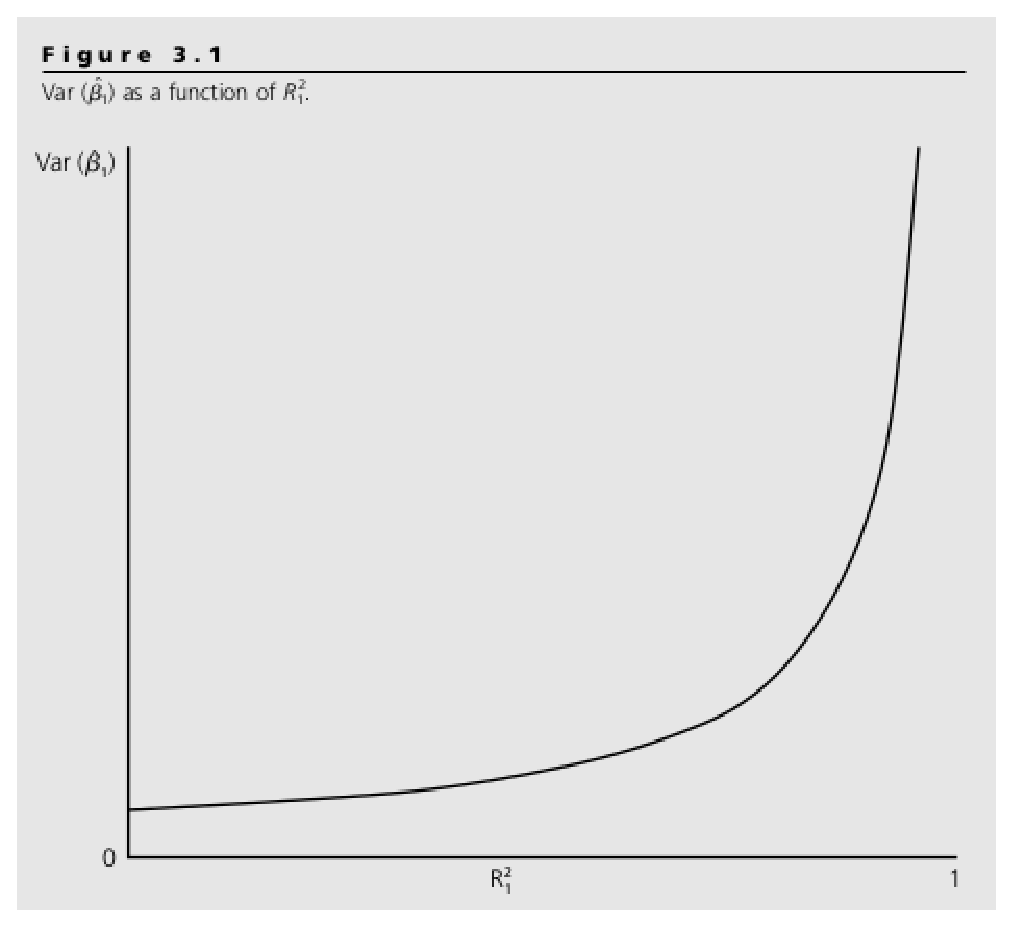
\includegraphics[scale = 0.5]{pictures/figure_3_1.eps}
\caption{$var[\hat{\beta}_j]$ jako funkce $R^2_j$}
\label{figure_3_1}
\end{figure} 

\subsection{Rozptyl v chybně specifikovaném regresním modelu}

Předpokládejme, že správně definovaný regresní model má podobu
\begin{equation}
y = \beta_0 + \beta_1 x_1 + \beta_2 x_2 + u.
\end{equation}
Dále předpokládejme, že namísto
\begin{equation}
\hat{y} = \hat{\beta}_0 + \hat{\beta}_1 x_1 + \hat{\beta}_2 x_2
\end{equation}
jsme odhadli model ve tvaru
\begin{equation}
\tilde{y} = \tilde{\beta}_0 + \tilde{\beta}_1 x_1.
\end{equation}
V takovém případě je $\tilde{\beta}_1$ zkreslené s výjimkou situace, kdy jsou $x_1$ a $x_2$ nekorelované. Pokud je zkreslení naším jediným 
kritériem výběru, pak preferujeme $\hat{\beta_1}$ před $\tilde{\beta}_1$. Pokud je však naším kritériem rozptyl odhadovaného parametru, pak 
můžeme naopak preferovat $\tilde{\beta}_1$ před $\hat{\beta_1}$, protože kromě situace, kdy $x_1$ a $x_2$ jsou nekorelované, je
\begin{equation}
var[\hat{\beta_1}] = \frac{\sigma^2}{SST_1(1 - R^2_1)}
\end{equation}
vždy větší než
\begin{equation}
var[\tilde{\beta}_1] = \frac{\sigma^2}{SST_1}.
\end{equation}
Proto bychom při rozhodování se mezi $\hat{\beta}_1$ a $\tilde{\beta}_1$ měli vzít v úvahu nejen velikost zkreslení, ale také velikost 
směrodatné odchylky odhadu. Je důležité si uvědomit, že směrodatná odchylka odhadu je také poplatná velikosti náhodného výběru. 
Další tak trochu skrytou skutečností je, že opominutím $x_2$ v regresním modelu se přesune část variability $x_2$ do 
rozptylu chyby $u$. Ta však není v rámci $var[\tilde{\beta}_1]$ zohledněna. Nižší variabilita $\tilde{\beta}_1$ tak může být poněkud zavádějící.

\subsection{Odhad $\sigma^2$}

OLS rezidua z odhadnutého modelu jsou definována jako
\begin{equation}
\hat{u}_i = y_i - \hat{\beta}_0 - \hat{\beta}_1 x_{i1} - \hat{\beta}_2 x_{i2} - ... - \hat{\beta}_k x_{ik}.
\end{equation}
Nezkreslený odhad jejich rozptylu $\sigma^2$ je pak roven
\begin{equation}
\hat{\sigma}^2 = \frac{\sum_{i = 1}^n \hat{u}_i^2}{n - k - 1} = \frac{SSR}{n - k - 1}.
\end{equation}
Člen $n - k - 1$ představuje počet stupňů volnosti obecného regresního modelu s $k$ vysvětlujícími veličinami odhadnutého nad náhodným 
výběrem o $n$ pozorováních. To, že úprava o počet stupňů volnosti je nezbytná, je zřejmé z podmínek prvního řádu 
pro OLS odhady. Tyto podmínky lze vyjádřit ve tvaru $\sum_{i = 2}^n \hat{u}_1 = 0$ a $\sum_{i = 1}^n x_{ij}\hat{u}_j = 0$, kde $j = 1, 2, ..., k$. Při 
odvození OLS odhadů je tak třeba aplikovat těchto $k+1$ omezení. To znamená, že pro daných $n - (k + 1)$ reziduí lze zbývajících $k + 1$ 
reziduí dopočíst na základě výše uvedených $k + 1$ omezení. Proto mají rezidua pouze $n - (k + 1)$ stupňů volnosti.
\begin{theorem}[Nestrannost odhadu $\sigma^2$]
Pokud jsou splněny Gauss-Markovy předpoklady MLR.1 až MLR.5, pak platí $E[\hat{\sigma}^2] = \sigma^2$.

\raggedleft{$\clubsuit$}
\end{theorem}
Směrodatná odchylka $\hat{\beta}_j$ je definována jako
\begin{equation}
sd(\hat{\beta}_j) = \frac{\sigma}{\sqrt{SST_j(1 - R^2_j)}}.
\end{equation}
Pokud $\sigma$ nahradíme jejím odhadem $\hat{\sigma}$, získáme tzv. směrodatnou chybu
\begin{equation}
se(\hat{\beta}_j) = \frac{\hat{\sigma}}{\sqrt{SST_j(1 - R^2_j)}}.
\end{equation}
Protože $se(\hat{\beta}_j)$ závisí na $\hat{\sigma}$, jedná se o náhodnou veličinu. Rovnice (3.43) není validním odhadem $sd(\hat{\beta}_j)$, 
pokud chyba $u$ vykazuje heteroskedasticitu.

\section{Efektivita OLS odhadu - Gauss-Markovova věta}

Při splnění předpokladů MLR.1 až MLR.5 jsou OLS odhady regresních parametrů nezkreslené. Při splnění těchto podmínek však kromě OLS odhadu existuje celá 
řada jiných nezkreslených lineárních odhadů. Nicméně OLS odhad je nejen nezkreslený, ale také efektivní, tj. má z těchto odhadů 
nejmenší rozptyl. Takovýto odhad nazýváme nejlepším nezkresleným lineárním odhadem (best linear unbiased estimator - BLUE).
\begin{theorem}[Gauss-Markovova věta]
Pokud jsou splněny Gauss-Markovovy předpoklady MLR.1 až MLR.5, pak platí $E[\hat{\sigma}^2] = \sigma^2$.

\raggedleft{$\clubsuit$}
\end{theorem}

Je třeba zdůraznit, že v případě heteroskedasticity je OLS 
odhad parametrů regresního modelu stále nezkreslený, nicméně již nemá nejmenší rozptyl mezi všemi možnými nezkreslenými lineárními odhady.

\chapter[Vícerozměrný regresní model \\ Testování hypotéz]{Vícerozměrný regresní model - testování hypotéz}

\section{Výběrové rozdělení OLS odhadů}

I při splnění všech Gauss-Markovových předpokladů může mít pravděpodobnostní rozdělení $\hat{\beta}_j$ v podstatě libovolný tvar. 
Lze dokázat, že pravděpodobnostní rozdělení $\hat{\beta}_j$ je závislé na pravděpodobnostním rozdělení chyb regresního modelu. 
Pro zjednodušení úvah o pravděpodobnostním rozdělení $\hat{\beta}_j$ předpokládejme, že pravděpodobnostní rozdělení chyb sleduje 
normální rozdělení; tento předpoklad nazýváme předpokladem normality.

\begin{assumption}[MLR.6 - normalita]
Chyba $u$ regresního modelu je nezávislá na vysvětlujících veličinách $x_1, x_2, ..., x_k$ a je normálně rozdělená s nulovou střední 
hodnotou a konstantním rozptylem $\sigma^2$, tj. $u \sim N(0, \sigma^2)$.

\raggedleft{$\clubsuit$}
\end{assumption}

\begin{figure}[htp]
\centering
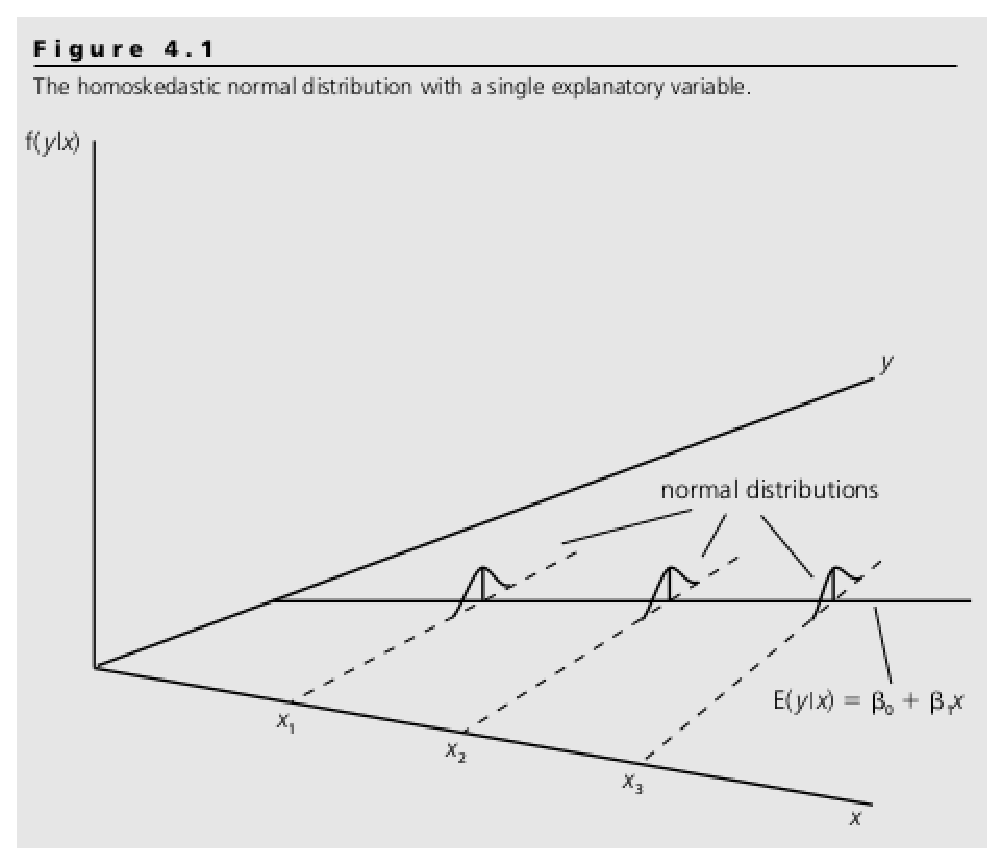
\includegraphics[scale = 0.5]{pictures/figure_4_1.eps}
\caption{Chyba $u$ jednoduchého regresního modelu, která sleduje normální rozdělení s nulovou střední hodnotou a konstantním rozptylem}
\label{figure_4_1}
\end{figure} 


Platnost předpokladu MLR.6 implikuje také platnost předpokladů MLR.4 a MLR.5. MLR.1 až MLR.6 jsou nazývány předpoklady klasického 
lineárního modelu (classical linear model (CLM) assumptions). Při splnění CLM předpokladů jsou OLS odhady $\hat{\beta}_0, 
\hat{\beta}_1, ..., \hat{\beta}_k$ efektivnějšími než by byly při splnění pouze Gauss-Markovových předpokladů. Lze dokázat, že tyto odhady 
jsou nestrannými odhady s minimálním rozptylem a to nejen mezi lineárními ale všemi typy odhadů.

Předpoklady klasického lineární modelu lze shrnout do rovnice
\begin{equation}
y|x_1, x_2, ..., x_k \sim N(\beta_0 + \beta_1 x_1 + \beta_2 x_2 + ... + \beta_k x_k).
\end{equation}
Protože chyba $u$ je součtem vlivu mnoha nejrůznějších faktorů ovlivňujících $y$, lze s odvoláním na centrální limitní větu 
předpokládat, že $u$ sleduje přibližně normální rozdělení. Hlavním problémem tohoto argumentu je implicitní předpoklad, že faktory, které 
vstupují do chyby $u$, jí ovlivňují odděleně a tudíž že tyto vlivy lze jednoduše sčítat. Pokud je $u$ komplikovanou funkcí těchto 
reziduálních faktorů, nemusí být tento předpoklad splněn. V některých případech lze problém předpokladu normality vyřešit, např. 
aplikací přirozeného logaritmu na vysvětlované popř. vysvětlující veličiny, která pravděpodobností rozdělení chyby $u$ normálnímu 
rozdělení přiblíží. Prozatím však jednoduše máme za to, že je předpoklad normality splněn.
\begin{theorem}[Normální výběrové rozdělení]
Pro odhad regresních parametrů na základě náhodného výběru při splnění CLM předpokladů MLR.1 až MLR.6 platí
\begin{equation}
\hat{\beta_j} \sim N(\beta_j, var[\hat{\beta}_j]),
\end{equation}
kde $var(\hat{\beta}_j)$ je dáno rovnicí (3.34). Proto $\frac{\hat{\beta}_j - \beta_j}{sd(\hat{\beta}_j)} \sim N(0, 1)$.

\raggedleft{$\clubsuit$}
\end{theorem}
Každé $\hat{\beta}_i$ lze zapsat ve tvaru $\hat{\beta}_j = \beta_j + \sum_{i = 1}^n w_{ij}u_i$, kde $w_{ij} = \frac{\hat{r}_{ij}}{SSR_j}$,
$\hat{r}_{ij}$ je $i$-té reziduum z regresního modelu $x_j$ na ostatní vysvětlující veličiny a $SSR_j$ je součtem čtverců reziduí této 
regrese. Protože $w_{ij}$ závisí pouze na nezávislých veličinách, lze s ní nakládat jako s nenáhodnou veličinou. $\hat{\beta}_j$ je tak lineární 
kombinací chyb $\{u_i: i = 1, 2, ..., n\}$ ve výběru. Vzhledem k předpokladu normality pak $\hat{\beta}_j$ sleduje normální rozdělení.

\section{Testování hypotézy jednoho parametru - $t$ test}
\begin{theorem}[$t$ rozdělení standardizovaných odhadů]
Při splnění CLM předpokladů MLR.1 až MLR.6 platí
\begin{equation}
\frac{\hat{\beta}_j - \beta}{se(\hat{\beta}_j)} \sim t_{n-k-1},
\end{equation}
kde $k + 1$ je počet odhadovaných parametrů regresního modelu $y = \beta_0 + \beta_1 x_1 + ... + \beta_k x_k + u$.

\raggedleft{$\clubsuit$}
\end{theorem}
$t$ rozdělení v (4.3) vychází ze skutečnosti, že konstanta $\sigma$ v $se(\hat{\beta}_j)$ byla nahrazena náhodnou veličinou $\hat{\sigma}$. 
Výše uvedená věta je extrémně důležitá, protože nám umožňuje testovat hypotézy týkající se parametru $\beta_j$. Pro účely 
testování hypotéz je pak definována tzv. $t$ statistika
\begin{equation}
t_{\hat{\beta}_j} \equiv \frac{\hat{\beta}_j}{se(\hat{\beta}_j)}.
\end{equation}

\subsection{Jednostranný test}

V rámci jednostranného testu zjišťujeme, zda-li je hodnota parametru $\beta_j$ menší či větší než určitá konstanta $c$. Nejčastěji se testuje 
$\beta_j$ proti $c = 0$, což znamená, že nulová a alternativní hypotéza mají podobu
\begin{equation}
H_0: \beta_j \le 0 ~~~~~~ H_1: \beta_j > 0,
\end{equation}
popř.
\begin{equation}
H_0: \beta_j \ge 0 ~~~~~~ H_1: \beta_j < 0.
\end{equation}
V prvním případě testujeme, zda-li je $\beta_j < 0$, kdežto ve druhém případě zda-li je $\beta_j > 0$. V prvním případě nulovou 
hypotézu zamítneme, pokud odpovídající $t$ statistika $t_{\beta_j} = \frac{\hat{\beta}_j}{se(\hat{\beta}_j)}$ splňuje podmínku
\begin{equation}
t_{\beta_j} > t_{n-k-1}^{1 - \alpha}
\end{equation}
a druhém případě, pokud splňuje podmínku
\begin{equation}
t_{\beta_j} < t_{n-k-1}^{\alpha},
\end{equation}
kde $t_{n-k-1}^{\alpha}$ představuje $\alpha$ kvantil Studentova rozdělení s $n-k-1$ stupni volnosti. Kvantil $\alpha$ též nazýváme hladinou významnosti.

\begin{figure}[htp]
\centering
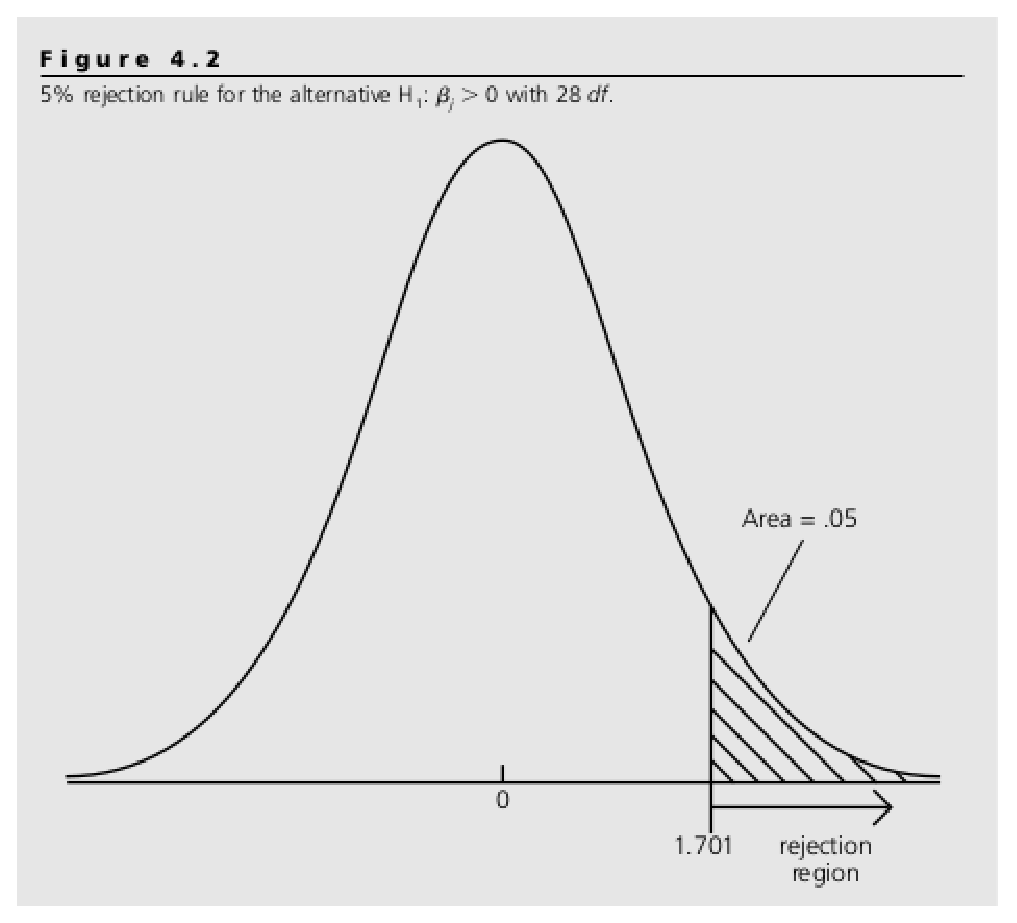
\includegraphics[scale = 0.5]{pictures/figure_4_2.eps}
\caption{Jednostranný test s alternativní hypotézou $H_1: \beta_j > 0$}
\label{figure_4_2}
\end{figure}

\begin{figure}[htp]
\centering
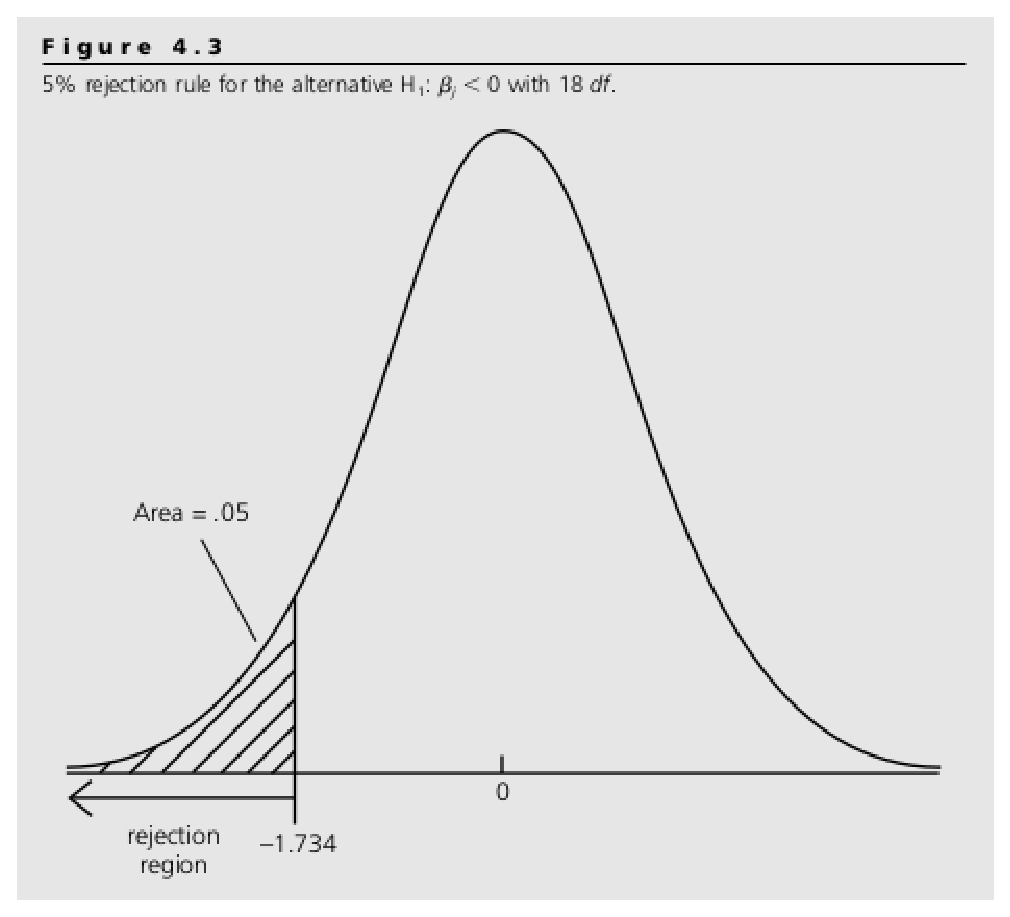
\includegraphics[scale = 0.5]{pictures/figure_4_3.eps}
\caption{Jednostranný test s alternativní hypotézou $H_1: \beta_j < 0$}
\label{figure_4_3}
\end{figure} 

Pokud je $c \ne 0$, pak se nulová a alternativní hypotéza změní na $H_0: \beta_j \le c, H_1: \beta_j > c$ popř. na $H_0: \beta_j \ge c, H_1: \beta_j < c$. Nulovou hypotézu zamítneme, pokud $t_{\beta_j} < t_{n-k-1}^{\alpha}$ popř. $t_{\beta_j} > t_{n-k-1}^{1 - \alpha}$, kde $t_{\beta_j} = \frac{\hat{\beta}_j - c}{se(\hat{\beta}_j)}$.

\subsection{Dvoustranný test}

V případě dvoustranného testu přejde nulová a alternativní hypotéza do tvaru
\begin{equation}
H_0: \beta_j = 0 ~~~~~~ H_1: \beta_j \ne 0,
\end{equation}
kdy nulovou hypotézu zamítneme pokud
\begin{equation}
|t_{\beta_j}| > t_{n-k-1}^{1 - \frac{\alpha}{2}}.
\end{equation}
Na rozdíl od jednostranného testu, který existuje ve dvou podobách, máme pouze jednu formu dvoustranného testu. V rámci nulové hypotézy pak testujeme, zda-li je $\beta_j$ rovno nule.

\begin{figure}[htp]
\centering
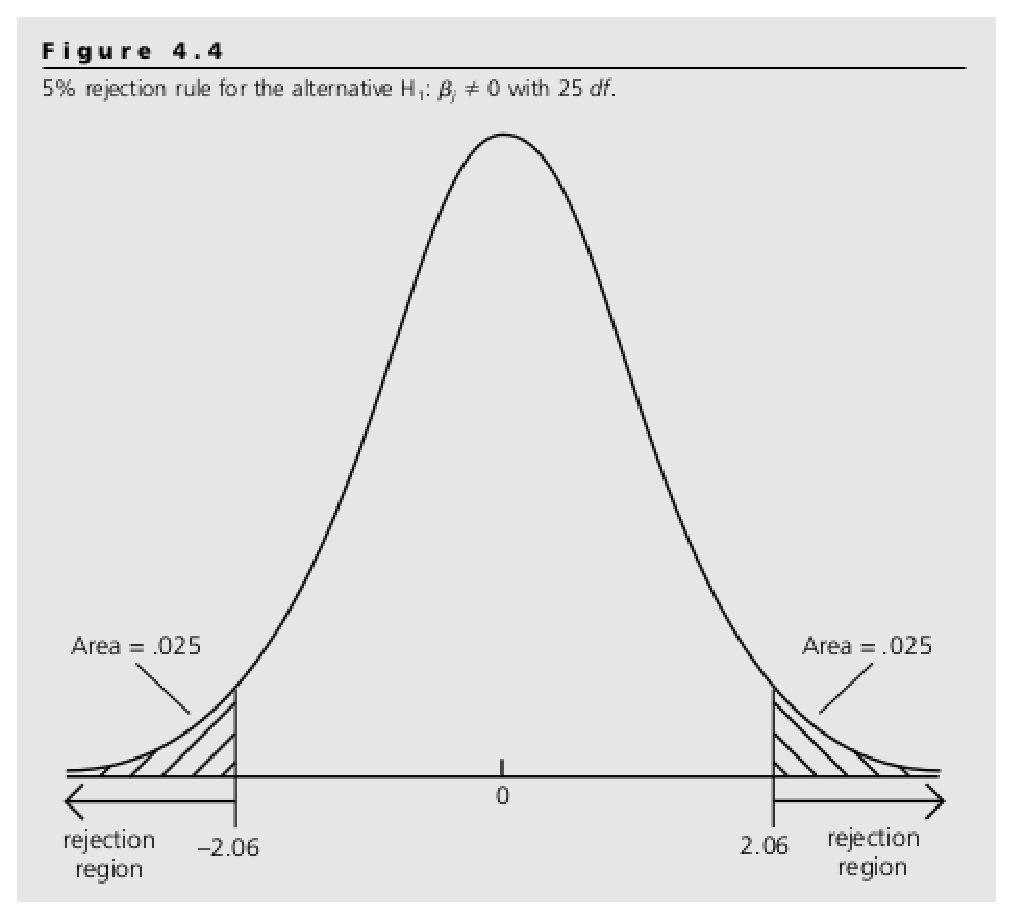
\includegraphics[scale = 0.5]{pictures/figure_4_4.eps}
\caption{Dvoustranný test s alternativní hypotézou $H_1: \beta_j \ne 0$}
\label{figure_4_4}
\end{figure} 

Podobně jako v případě jednostranného testu lze dvoustranný test snadno zobecnit na případy, kdy $c \ne 0$. V tomto případě nulová a alternativní hypotéza přejde na $H_0: \beta_j = c, H_1: \beta_j \ne c$, kdy nulovou hypotézu zamítneme, pokud $|t_{\beta_j}| > t_{n-k-1}^{1 - \frac{\alpha}{2}}$, kde $t_{\beta_j} = \frac{\hat{\beta}_j - c}{se(\hat{\beta}_j)}$.

\subsection{p-hodnota (p-value)}

Při testování hypotéz je třeba zvolit hladinu významnosti $\alpha$. Je třeba zdůraznit, že neexistuje žádná ``správná'' hladina 
významnosti. Nicméně pro danou hodnotu $t$ statistiky si můžeme položit otázku, jaká je nejnižší hladina významnosti, pro kterou je 
nulová hypotéza zamítnuta. Tuto hladinu významnosti nazýváme p-hodnotou. Z této definice je zřejmé, že nízká p-hodnota je argumentem pro 
zamítnutí nulové hypotézy, zatímco vysoká p-hodnota je argumentem pro přijetí nulové hypotézy. Jinými slovy, je-li námi zvolená 
hladina významnosti rovna $\alpha$, pak pro $p-hodnota < \alpha$ nulovou hypotézu zamítneme.

\subsection{Interval spolehlivosti}

V řadě případů je žádoucí zjistit interval, ve kterém se parametr $\beta_j$ s určitou pravděpodobností nachází. S ohledem na větu (4.2) víme, že
\begin{equation}
\frac{\hat{\beta}_j - \beta}{se(\hat{\beta}_j)} \sim t_{n - k -1}.
\end{equation}
Pokud tedy chceme najít interval, ve kterém se s pravděpodobností $1 - \alpha$ bude nacházet parametr $\beta$, pak prostou modifikací výše 
uvedeného získáme
\begin{equation}
\hat{\beta}_j - t_{n - k -1}^{1 - \frac{\alpha}{2}} \le \beta \le \hat{\beta}_j + t_{n - k -1}^{1 - \frac{\alpha}{2}}.
\end{equation}
Pokud zkombinujeme (4.10) s (4.11) a výsledek porovnáme s (4.12), je zřejmé, že interval spolehlivosti a dvoustranný $t$ test jsou postaveny na 
stejném logickém základě.

\subsection{Testování hypotéz zahrnujících lineární kombinaci vícero parametrů}

Uvažujme jednoduchý regresní model, ve kterém provádíme regresi logaritmu příjmu na počet roků strávených na bakalářském a magisterském 
studijním oboru a počtu roků praxe, tj.
\begin{equation}
ln(wage) = \beta_0 + \beta_1 bac + \beta_2 mag + \beta_3 exp + u.
\end{equation}
Předpokládejme, že chceme testovat $H_0: \beta_1 = \beta_2$ proti $H_1: \beta_1 < \beta_2$, tj. zda-li jeden rok studia bakalářského oboru 
zvýší mzdu o stejné procento jako rok studia magisterského oboru. Nulovou a alternativní hypotézu lze přepsat do tvaru $H_0: \beta_1 - 
\beta_2 = 0$ a $H_1: \beta_1 - \beta_2 < 0$. To znamená, že namísto jednoho parametru, testujeme lineární kombinaci dvou parametrů. Je 
důležité si uvědomit, že pravděpodobnostní rozdělení odhadu každého z parametrů sleduje při splnění CLM předpokladů Studentovo 
rozdělení stejně jako každá jejich lineární kombinace. Proto jsme pro $\hat{\theta} = \hat{\beta}_1 - \hat{\beta}_2$ teoreticky schopni zkonstruovat $t$ statistiku
\begin{equation}
t = \frac{\hat{\theta} - \theta}{se(\hat{\theta})},
\end{equation}
kde $se(\hat{\theta}) = \sqrt{var[\hat{\beta}_1] + var[\hat{\beta}_1] - 2cov[\hat{\beta}_1, \hat{\beta}_2]}$ a tu následně použít pro účely 
testování nulové hypotézy. V praxi bohužel tento postup naráží na neznalost $cov[\hat{\beta}_1, \hat{\beta}_2]$. Tento problém však lze 
relativně snadno obejít přeformulováním původního regresního modelu do tvaru
\begin{equation}
ln(wage) = \beta_0 + \theta bac + \beta_2 (bac + mag) + \beta_3 exp + u.
\end{equation}
Po této upravě provedeme odhad modelu pomocí OLS a následně aplikujeme standardní dvoustranný $t$ test na parametr $\theta$, kde testujeme 
$H_0: \theta = 0$ proti $H_1: \theta \ne 0$.

Analogický postup lze použít také v případech jiných lineárních kombinací, např. při 
testování nulové hypotézy $H_0: \beta_1 = 0.75 \beta_2$ proti alternativní hypotéze $H_1: \beta_1 \ne 0.75 \beta_2$. Kromě dvoustranných 
hypotéz lze testovat také jednostranné hypotézy.

\section{Testování vícero lineárních omezení - $F$ test}

\subsection{Testování významnosti vícero parametrů}

Předpokládejme, že chceme testovat, zda-li má určitá skupina vysvětlujících veličin vliv na vysvětlovanou veličinu. Uvažujme 
vícerozměrný regresní model
\begin{equation}
y = \beta_0 + \beta_1 x_1 + \beta_2 x_2 + \beta_3 x_3 + \beta_4 x_4 + \beta_5 x_5 + u,
\end{equation}
pro který budeme testovat nulovou hypotézu
\begin{equation}
H_0: \beta_3 = 0, \beta_4 = 0, \beta_5 = 0.
\end{equation}
Hypotézu v tomto tvaru nazýváme vícenásobnou 
popř. sdruženou hypotézou. Alternativní hypotéza $H_1: \textit{nepravdivá} ~~ H_0$ je platná, pokud alespoň jeden parametr z $\beta_3$, $\beta_4$ nebo 
$\beta_5$ je různý od nuly.

Na první pohled by se mohlo zdát, že (4.17) můžeme testovat parametr po parametru s využitím klasického dvoustranného $t$ testu. Nicméně 
jednotlivé $t$ testy se zaměřují vždy jen na ``svůj'' parametr. Pokud bychom tedy hypotézu (4.17) testovali pomocí série $t$ testů, byli bychom příliš 
konzervativní. Intuitivně lze odhadnout, že sdružený test by mohl být založen na změně $R^2$. Z předchozího textu víme, že 
přidáním vysvětlujících veličin se zvýší $R^2$ modelu. Otázkou tedy je, zda-li je toto zvýšení dostatečné na to, aby přidání 
těchto vysvětlujících veličin ospravedlnilo.

Uvažujme regresní model
\begin{equation}
y = \beta_0 + \beta_1 x_1 + ... + \beta_k x_k + u.
\end{equation}
Pro účely následujícího textu budeme tento model označovat jako neomezený (unrestricted model). Uvažujme nulovou hypotézu
\begin{equation}
H_0: \beta_{k - q + 1} = 0, ..., \beta_k = 0.
\end{equation}
Pokud z původního neomezeného modelu vypustíme vysvětlující veličiny $\beta_{k - q + 1}, ..., \beta_k$, získáme tzv. omezený model 
(restricted model) ve tvaru
\begin{equation}
y = \beta_0 + \beta_1 x_1 + ... + \beta_{k - q}x_{k - q} + u.
\end{equation}
Definujme tzv. $F$ statistiku
\begin{equation}
F \equiv \frac{\frac{SSR_r - SSR_{ur}}{q}}{\frac{SSR_{ur}}{n - k - 1}},
\end{equation}
kde $SSR_r$ je reziduální součet čtverců omezeného modelu, $SSR_{ur}$ je reziduální součet čtverců neomezeného modelu a $q$ představuje 
rozdíl stupňů volnosti mezi neomezeným a omezeným modelem (což odpovídá počtu testovaných parametrů), tj. $q = df_{ur} - df_{r}$. Připomeňme, že 
$R^2 = 1 - \frac{SSR}{SST}$, kde $SSR = \sum_{i = 1}^n \hat{u}_i^2$ a $SST = \sum_{i = 1}^n (y_i - \overline{y})^2$.

$F$ statistika sleduje $F$ rozdělení s $(q, n - k - 1)$ stupni volnosti, tj.
\begin{equation}
F \sim F_{q, n - k - 1}.
\end{equation}
Nulovou hypotézu tedy zamítneme ve prospěch alternativní hypotézy, pokud
\begin{equation}
F > F_{q, n - k - 1}^{\alpha},
\end{equation}
kde $\alpha$ představuje námi zvolenou hladinu významnosti. Pokud je nulová hypotéza zamítnuta, říkáme, že vysvětlující veličiny $x_{k 
- q + 1, ..., x_k}$ jsou sdruženě statisticky významné. V praxi se může stát, že ačkoliv jsou jednotlivé vysvětlující veličiny 
individuálně statisticky nevýznamné, jsou sdruženě statisticky významné. Poněkud překvapivě však může nastat i opačná situace, tj. 
pokud ke skupině statisticky nevýznamných veličin přidáme jednu statisticky významnou, můžeme dojít k závěru, že skupina těchto 
vysvětlujících veličin je jako celek sdruženě statisticky nevýznamná.

\subsection{Vztah mezi $F$ a $t$ testem}

Lze dokázat, že $F$ statistika pro testování jednoho parametru je rovna čtverci odpovídající $t$ statistiky. Protože $t_{n - k - 1}^2$ a 
$F_{1, n - k - 1}$ sledují stejné pravděpodobnostní rozdělení, vedou obě statistiky v případě dvoustranného testu k shodným závěrům.

\subsection{$R^2$ forma $F$ statistiky}

Připomeňme, že $SSR_r = SST(1 - R_r^2)$ a $SSR_{ur} = SST(1 - R_{ur}^2)$. Dosazením do (4.21) získáme tzv. $R^2$ formu $F$ statistiky.
\begin{equation}
F = \frac{\frac{R_{ur}^2 - R_t^2}{q}}{\frac{(1 - R_{ur}^2)}{n - k -1}} = \frac{\frac{R_{ur}^2 - R_r^2}{q}}{\frac{(1 - R_{ur}^2)}{n - k - 1}}
\end{equation}

\subsection{Výpočet p-hodnoty $F$ testu}

P-hodnotu $F$ testu definujeme jako
\begin{equation}
p-hodnota = P(\mathcal{F} > F),
\end{equation}
kde $\mathcal{F}$ představuje náhodnou veličinu z $F$ rozdělení s $(q, n - k - 1)$ stupni volnosti a $F$ je hodnota $F$ statistiky. P-hodnota pak 
představuje pravděpodobnost, že budeme pozorovat danou hodnotu $F$ statistiky za předpokladu platnosti nulové hypotézy. Pokud je p-hodnota 
nižší než námi zvolená hladina významnosti $\alpha$, nulovou hypotézu zamítneme.

\subsection{Test celkové statistické významnosti regresního modelu}

Uvažujme regresní model (4.18), nulovou hypotézu
\begin{equation}
H_0: \beta_1 = \beta_2 = ... = \beta_k = 0
\end{equation}
a alternativní hypotézu, která říká, že alespoň jeden parametr $\beta_j$ je různý od nuly. Tento test nazýváme testem celkové 
statistické významnosti regresního modelu. Logika testu je stejná jako v případě klasického $F$ testu s tím, že omezený model má tvar
\begin{equation}
y = \beta_0 + u.
\end{equation}
Protože $R^2$ regresního modelu (4.27) je rovno nule, zjednoduší se $F$ statistika do tvaru
\begin{equation}
F = \frac{\frac{R^2}{k}}{\frac{1 - R^2}{n - k - 1}}
\end{equation}

\subsection{Testování obecných lineárních omezení}

Uvažujme regresní model
\begin{equation}
y = \beta_0 + \beta_1 x_1 + \beta_2 x_2 + \beta_3 x_3 + \beta_4 x_4 + u
\end{equation}
a nulovou hypotézu
\begin{equation}
H_0: \beta_1 = 1, \beta_2 = 0, \beta_3 = 0, \beta_4 = 0.
\end{equation}
Omezený model získáme dosazením omezení z nulové hypotézy do původního modelu. Omezený model má pak v našem konkrétním případě tvar
\begin{equation}
y - x_1 = \beta_0 + u.
\end{equation}
Pro účely výpočtu $F$ statistiky nemůžeme používat (4.24), protože závislá veličina v modelu (4.31) není $y$ ale $y - x_1$. Proto je 
třeba použít (4.31).

\chapter[Vícerozměrný regresní model \\ Asymptotické vlastnosti OLS odhadů]{Vícerozměrný regresní model - asymptotické vlastnosti OLS odhadů}

Asymptotické vlastnosti OLS odhadů představují jejich charakteristiky platné pro výběry velkého rozsahu. V předchozím textu jsme např. zmínili, že 
při splnění předpokladů MLR.1 až MLR.6 sleduje $t$ statistika Studentovo rozdělení. S rostoucí velikostí náhodného výběru se však 
pravděpodobnostní rozdělení $t$ statistiky asymptoticky blíží Studentovu rozdělení i v případech, kdy není splněn předpoklad normality MLR.6.

\section{Konzistentnost odhadu}

Nechť $\hat{\beta}_j$ představuje OLS odhad regresního parametru $\beta_j$. Pro každý náhodný výběr velikosti $n$ sleduje $\hat{\beta}_j$ určité pravděpodobnostní rozdělení. Protože při splnění 
předpokladů MLR.1 až MLR.4 je $\hat{\beta}_j$ nezkresleným odhadem $\beta_j$, má toto pravděpodobnostní rozdělení střední hodnotu 
$\beta_j$. Jestliže je odhad $\hat{\beta}_j$ konzistentní, pak se jeho rozptyl s rostoucím $n$ zmenšuje. S tím, 
jak se $n$ blíží nekonečnu, ``kolabuje'' pravděpodobnostní rozdělení $\hat{\beta}_j$ do bodu $\beta_j$. Konzistentnost tedy představuje 
minimální požadavek na odhad - pokud se s využitím stále většího náhodného výběru neblíží $\hat{\beta}_j$ skutečné hodnotě 
$\beta_j$, pak používáme nevhodnou metodu odhadu.

\begin{theorem}[Konzistentnost OLS odhadu]
Při splnění předpokladů MLR.1 až MLR.4 je $\hat{\beta}_j$ konzistentním odhadem $\beta_j$ pro všechna $j = 0, 1, ..., k$.

\raggedleft{$\clubsuit$}
\end{theorem}

\begin{proof}
Platnost
 výše uvedené věty demonstrujme na příkladu $\beta_1$. Odhad $\hat{\beta}_1$ lze vyjádřit ve tvaru
\begin{equation}
\hat{\beta}_1 = \frac{\sum_{i=1}^n(x_{i1} - \overline{x}_1)y_i}{\sum_{i = 1}^n (x_{i1} - \overline{x}_1)^2} = \beta_1 + \frac{\frac{\sum_{i=1}^n(x_{i1} 
- \overline{x}_1)u_i}{n}}{\frac{\sum_{i = 1}^n (x_{i1} - \overline{x}_1)^2}{n}}.
\end{equation}
S využitím vztahů $var[x_1] \ne 0$, což vyžaduje MLR.3, a $cov[x_1, u] = 0$, což vyplývá z MLR.4, získáme
\begin{equation}
plim ~ \hat{\beta}_j = \beta_1 + \frac{cov[x_1, u]}{var[x_1]} = \beta_1.
\end{equation} 

\raggedleft{$\clubsuit$}
\end{proof}

\begin{assumption}[MLR.4' - nulová střední hodnota a korelace]
$E[u] = 0$ a $cov[x_j, u] = 0$ pro všechna $j = 0, 1, ..., k$.

\raggedleft{$\clubsuit$}
\end{assumption}

Předpoklad MLR.4' je slabší než předpoklad MLR.4, protože platnost MLR.4 implikuje platnost MLR.4'. Jedním ze způsobů, jak charakterizovat 
$E[u|x_1, ..., x_k] = 0$ je, že libovolná funkce vysvětlujících veličin je nekorelovaná s $u$. Předpoklad MLR.4' však pouze vyžaduje, aby 
každé jednotlivé $x_j$ bylo nekorelované s $u$. Na druhou stranu předpoklad MLR.4' je v porovnání s MLR.4 ``přirozenější'', 
protože nás vede přímo k OLS odhadům. Navíc, pokud v praxi mluvíme o porušení předpokladu MLR.4 máme většinou na mysli nesplnění $cov[x_j, 
u] = 0$. Předpoklad $E[u] = 0$ zajišťuje, že správně modelujeme populační regresní funkci. To znamená, že při splnění MLR.4 můžeme psát
\begin{equation}
E[y|x_1, ..., x_k] = \beta_0 + \beta_1 x_1 + ... + \beta_k x_k.
\end{equation}
Pokud bychom však namísto MLR.4 předpokládali pouze MLR.4', pak $\beta_0 + \beta_1 x_1 + ... + \beta_k x_k$ nemusí představovat populační 
regresní funkci, protože může existovat nelineární funkce $x_j$, např. $x_j^2$, která je korelovaná s $u$. To by znamenalo, že jsme z modelu 
vypustili nelinearity, které nám mohly pomoci lépe vysvětlit $y$. Pokud bychom si těchto nelinearit byli vědomi, pak bychom je do regresního 
modelu zařadili.

\subsection{Odvození nekonzistentnosti OLS odhadů}

Jestliže je chyba $u$ korelována s libovolnou vysvětlující veličinou, pak jsou OLS dohady zkreslené a nekonzistentní. Nekonzistentnost 
bohužel znamená, že tyto odhady zůstávají zkreslené i při rostoucí velikosti náhodného výběru. Nekonzistentnost odhadu $\hat{\beta}_j$ je
\begin{equation}
plim ~ \hat{\beta}_j - \beta_j = \frac{cov[x_j, u]}{var[x_j]}.
\end{equation}
Pokud je korelace mezi $x_j$ a $u$ zanedbatelná, může být zanedbatelná i míra nekonzistentnosti. V praxi bohužel zpravidla tuto korelaci 
neznáme, protože neznáme $u$.

(5.4) lze použít pro odvození vztahu pro zkreslení z titulu opomenutí relevantní vysvětlující proměnné, kterou jsme diskutovali v 
kapitole 3. Předpokládejme, že skutečný regresní model má tvar
\begin{equation}
y = \beta_0 + \beta_1 + \beta_2 + v,
\end{equation}
kde $v$ má nulovou střední hodnotu, konstantní rozptyl a je nekorelované s $x_1$ a $x_2$. Pokud však z nějakého důvodu budeme uvažovat model
\begin{equation}
y = \beta_0 + \beta_1 x_1 + u,
\end{equation}
pak $u = \beta_2 x_2 + v$. Jestliže odhad sklonu v jednoduchém regresním modelu označíme jako $\tilde{\beta}_1$, pak
\begin{equation}
plim ~ \tilde{\beta}_1 = \beta_1 + \beta_2 \delta_1,
\end{equation}
kde $\delta_1 = \frac{cov[x_1, x_2]}{var[x_1]}$. To znamená, že s tím, jak poroste velikost náhodného výběru, se OLS odhad bude stále více 
blížit $\beta_1 + \beta_2 \delta_1$. Z tohoto pohledu tedy lze nekonzistentnost chápat obdobně jako zkreslení.

V případě obecného vícerozměrného regresního modelu je odhad směru a velikosti nekonzistentnosti mnohem složitější, stejně jako je 
mnohem složitější odvodit směr a velikost zkreslení odhadu. Je třeba mít na paměti, že pokud je např. $x_1$ korelováno s $u$, zatímco 
ostatní vysvětlující proměnné nikoliv, jsou nekonzistentní odhady všech parametrů regresního modelu, nikoliv pouze odhad $\hat{\beta}_1$.

\subsection{Asymptotická normalita OLS odhadů a výběr velkého rozsahu}

Věta (4.1) tvrdí, že pokud jsou splněny předpoklady MLR.1 až MLR.6, sleduje odhad $\hat{\beta}_j$ normální rozdělení. Tento závěr je 
základem pro odvození $t$ a $F$ statistik, které jsou velmi často používány v ekonometrii. Platnost věty je zásadním způsobem závislá na 
předpokladu normality, tj. předpokladu, že chyba $u$ sleduje normální rozdělení. Pokud jsou chyby $u_1, u_2, ..., u_n$ náhodnými výběry z 
jiného pravděpodobnostního rozdělení, pak $\hat{\beta}_j$ normální rozdělení nesleduje. To znamená, že $t$ statistika nesleduje Studentovo 
rozdělení a $F$ statistika nesleduje $F$ rozdělení.

Předpoklad MLR.6 ve své podstatě říká, že $y$ pro dané $x_1, x_2, ..., x_n$ sleduje normální rozdělení. Protože $y$ na rozdíl od $u$ 
známe, je mnohem jednodušší se zabývat pravděpodobnostním rozdělení $y$ než $u$. Mnohdy však $y$ normální 
rozdělení nesleduje. Jako příklad můžeme uvažovat regresní model, ve kterém se budeme snažit vysvětlit počet roků strávených v 
nápravných zařízeních pomocí dosaženého vzdělání, roční výše příjmů a rodinné příslušnosti. Protože pro drtivou většinu 
populace platí $y = 0$, a protože z logiky věci vyplývá $y \ge 0$, nemůže $y$ sledovat normální rozdělení. V řadě případů však lze s 
ohledem na centrální limitní větu předpokládat, že ačkoliv $y$ nesleduje normální rozdělení, OLS odhady se pro výběry velkého rozsahu 
asymptoticky blíží normálnímu rozdělení.

Nicméně normalita nemá vliv ani na nezkreslenost OLS odhadů a ani na skutečnost, že OLS je při splnění Gauss-Markovových předpokladů 
BLUE. Nicméně přesné testování hypotéz založené na $t$ a $F$ statistice vyžaduje platnost MLR.6.

\begin{theorem}[Asymptotická normalita OLS odhadů]
Při splnění předpokladů MLR.1 až MLR.5 platí následující.
\begin{itemize}
\item $\sqrt{n} (\hat{\beta}_j - \beta_j) \sim^a N(0, \frac{\sigma^2}{a_j^2})$, kde $\frac{\sigma^2}{a_j^2} > 0$ je asymptotický 
rozptyl $\sqrt{n}(\hat{\beta}_j - \beta_j)$. Pro odhady sklonu platí $a_j^2 = plim ~ \left(\frac{1}{n} \sum_{i = 1}^n \hat{r}_{ij}^2 \right)$, kde 
$\hat{r}_{ij}$ jsou rezidua z regrese $x_j$ na ostatní vysvětlující proměnné. O $\hat{\beta}_j$ říkáme, že je asymptoticky normálně rozdělené.
\item $\hat{\sigma}^2$ je konzistentním odhadem $\sigma^2 = var[u]$.
\item Pro každé $j$ platí
\begin{equation}
\frac{\hat{\beta}_j - \beta_j}{se(\hat{\beta}_j)} \sim^a N(0, 1),
\end{equation}
kde $se(\hat{\beta}_j)$ je běžná směrodatná odchylka OLS odhadu.
\end{itemize}

\raggedleft{$\clubsuit$}
\end{theorem}

Věta (5.2) je velmi důležitá, protože nám umožňuje odhlédnout od předpokladu MLR.6. Jedinou podmínkou pro pravděpodobnostní rozdělení 
$u$ je tak konečný rozptyl, nulová podmíněná střední hodnota a homoskedasticita.

Připomeňme, že $t$ statistiku jsme původně definovali jako
\begin{equation}
\frac{\hat{\beta}_j - \beta_j}{se(\hat{\beta}_j)} \sim t_{n - k - 1},
\end{equation}
kdežto výše uvedená věta tvrdí
\begin{equation}
\frac{\hat{\beta}_j - \beta_j}{se(\hat{\beta}_j)} \sim^a N(0, 1).
\end{equation}
V obou případech se však jedná pouze o aproximaci. Pokud je splněno MLR.6, pak $t$ statistika sleduje Studentovo rozdělení pro libovolnou velikost vzorku. Pro $n - k - 
1 \ge 20$ však z praktického hlediska není mezi normálním a Studentovým rozdělením zásadnější rozdíl, a proto lze (5.9) a (5.10) 
používat zaměnitelně. Pokud však $u$ nesleduje normální rozdělení, pak pro výběry malého rozsahu může být Studentovo rozdělení špatnou 
aproximací. V praxi však bohužel neexistuje přesné vodítko pro určení velikosti vzorku, pro který lze považovat aproximaci (5.9) a (5.10) 
za přijatelnou. Pokud však $var[y| x_1, x_2, ..., x_k]$ není konstantní, pak je obvyklá $t$ statistika neplatná bez ohledu na velikost vzorku, 
protože v podmínkách heteroskedasticity nelze centrální limitní větu aplikovat.

Rozptyl odhadu $\hat{\beta}_j$ je definován jako
\begin{equation}
se(\hat{\beta}_j)^2 = \frac{\hat{\sigma}^2}{SST_j(1 - R_j^2)}.
\end{equation}
S tím, jak roste velikost náhodného výběru se $\hat{\sigma}^2$ blíží konstantě $\sigma^2$, zatímco $1 - R_j^2$ konverguje k určitému 
číslu mezi nulou a jedničkou. $SST_j$ roste přibližně stejně rychle jako 
velikost výběru, tj. $SST_j \approx n \sigma_j^2$, kde $\sigma_j^2$ je populační rozptyl vysvětlující veličiny $x_j$. 
$se(\hat{\beta}_j)^2$ se tak blíží nule rychlostí $1/n$ s tím, jak roste velikost náhodného výběru. Proto jsou výběry velkého rozsahu pro odhad OLS 
parametrů vždy vhodnější.

Pokud $u$ nesleduje normální rozdělení, pak se $se(\hat{\beta}_j)$ z (5.11) někdy nazývá asymptotická směrodatná odchylka a odpovídající 
$t$ statistika asymptotickou $t$ statistikou.

S ohledem na výše uvedené lze napsat
\begin{equation}
se(\hat{\beta}_j) \approx \frac{c_j}{\sqrt{n}},
\end{equation}
kde $c_j$ je kladná konstanta nezávislá na velikosti náhodného výběru. Jinými slovy, velikost $se(\hat{\beta}_j)$ se zmenšuje s inverzí druhé 
odmocniny velikosti náhodného výběru.

Asymptotická normalita OLS odhadů také implikuje, že $F$ statistika pro náhodné výběry velkého rozsahu přibližně sleduje $F$ rozdělení.

\subsection{Statistika Lagrangova multiplikátoru}

Uvažujme regresní model
\begin{equation}
y = \beta_0 + \beta_1 x_1 + ... + \beta_k x_k + u,
\end{equation}
pro který testujeme nulovou hypotézu
\begin{equation}
H_0: \beta_{k - q + 1} = 0, ..., \beta_k = 0.
\end{equation}
Na rozdíl od $F$ testu se v případě testu založeném na statistice Lagrangova multiplikátoru zaobíráme pouze odhadem omezeného modelu
\begin{equation}
y = \tilde{\beta}_0 + \tilde{\beta}_1 x_1 + ... + \tilde{\beta}_{k - q} x_{k - q} + \tilde{u}.
\end{equation}
Pokud mají vysvětlující veličiny $x_{k  - q - 1}$ až $x_k$ skutečně nulový sklon, je $\tilde{u}$ (alespoň přibližně) nekorelované z 
každou z těchto veličin. Proto použijeme pomocný regresní model
\begin{equation}
\tilde{u} = \alpha_0 + \alpha_1 x_1 + ... + \alpha_k x_k + v,
\end{equation}
kde očekáváme, že $R^2$ odhadnutého modelu (5.16) je blízké nule. Při platnosti nulové hypotézy $H_0: R^2 = 0$ sleduje $nR^2$ rozdělení $\chi^2$ 
s $q$ stupni volnosti, tj. nulovou hypotézu zamítneme, pokud $nR^2 > \chi_{1 - \alpha}^2$, kde $\alpha$ je námi zvolená hladina významnosti.

Na rozdíl od $F$ testu nehraje v případě statistiky Langrangova multiplikátoru počet stupňů volnosti zásadnější roli. Důvodem je 
asymptotické chování této statistiky.

Závěry učiněné na základě $F$ statistiky a statistiky Lagrangových multiplikátorů se mohou pro výběry malého rozsahu lišit. V 
případě výběru velkého rozsahu jsou rozdíly velice výjimečné.

\subsection{Asymptotická efektivita OLS odhadů}

Při splnění Gauss-Markovových předpokladů jsou OLS odhady nejen asymptoticky normální ale také asymptoticky efektivní.

Uvažujme jednoduchý regresní model
\begin{equation}
y = \beta_0 + \beta_1 x + u,
\end{equation}
kde $u$ splňuje MLR.4, tj. $E[u|x] = 0$. Nechť $g(x)$ je libovolná funkce $x$, např. $g(x) = x^2$. Pak je $u$ nekorelované s $g(x)$. Definujme 
$z_i = g(x_i)$. Pak
\begin{equation}
\tilde{\beta}_1 = \frac{\sum_{i = 1}^n(z_i - \overline{z})y_i}{\sum_{i = 1}^n (z_i - \overline{z})x_i}
\end{equation}
je konzistentní odhad $\beta_1$ za předpokladu, že $g(x)$ a $x$ jsou korelované\footnote{$g(x)$ a $x$ mohou být nekorelované, protože korelace 
je mírou lineární nikoliv obecné závislosti.}. Jestliže $cov[z, x] \ne 0$, tj. $z$ a $x$ jsou korelované, získáme
\begin{equation}
plim ~ \tilde{\beta}_1 = \beta_1 + \frac{cov[z, u]}{cov[z, x]} = \beta_1,
\end{equation}
protože $cov[z, u] = 0$ pro MLR.4. Lze ukázat, že $\sqrt{n}(\tilde{\beta}_1 - \beta_1)$ je asymptoticky normální s nulovou střední hodnotou a 
asymptotickým rozptylem $\sigma^2 \frac{var[z]}{(cov[z, x])^2}$. Asymptotický rozptyl OLS odhadů získáme pro $z = x$, který je v tomto 
případě roven $cov[z,x] = cov[x,x] = var[x]$. Asymptotický rozptyl $\sqrt{n}(\hat{\beta}_1 - \beta_1)$ je pak $\sigma^2 \frac{var[x]}{var[x]^2} = 
\frac{\sigma^2}{var[x]}$. Cauchy-Schwartzova nerovnost implikuje $(cov[z, x])^2 \le var[z]var[x]$, což znamená, že asymptotický rozptyl 
$\sqrt{n}(\hat{\beta}_1 - \beta_1)$ není větší než rozptyl $\sqrt{n}(\tilde{\beta}_1 - \beta_1)$. Jinými slovy OLS odhad má menší 
asymptotický rozptyl než libovolný odhad ve tvaru (5.18). Pokud však není splněn předpoklad homoskedasticity, pak mohou existovat odhady 
(5.17), které mají menší asymptotický rozptyl než odpovídající OLS odhad.

\begin{theorem}[Asymptotická efektivnost OLS odhadů]
Jestliže jsou splněny Gauss-Markovovy předpoklady, pak pro obecný odhad $\tilde{\beta}_j$ a odpovídající OLS odhad $\hat{\beta}_j$ platí, 
že $\hat{\beta}_j$ má asymptotický rozptyl menší nebo roven asymptotickému rozptylu $\tilde{\beta}_j$, tj. $avar[\sqrt{n}(\hat{\beta}_j - \beta_j)] \le avar[\sqrt{n}(\tilde{\beta}_j - \beta_j)]$

\raggedleft{$\clubsuit$}
\end{theorem}

\chapter[Vícerozměrný regresní model \\ Další témata]{Vícerozměrný regresní model - další témata}

\section{Efekt změny měrné veličiny na OLS statistiky}

Pokud jsou veličiny přeškálovány, např. převodem z metrů na kilometry, změní se odhady regresních parametrů, jejich směrodatné 
odchylky, intervaly spolehlivosti a $t$ a $F$ statistiky způsobem, který zachovává všechny efekty měření a výsledky testování. Také 
hodnota $R^2$ je změnou měrné jednotky nedotčena, ačkoliv součet čtverců reziduí SSR a standardní směrodatná odchylka regrese SER se změní.

Pokud je závislá proměnná vyjádřena v logaritmické formě, pak změna měrné jednotky nemá vliv na odhad sklonů. Dojde však ke změně z 
$ln(y_i)$ na $ln(c_1 y_i) = ln(c_1) + ln(y_i)$, změní se průsečík z $\beta_0$ na $\beta_0 + ln(c_1)$.

Někdy je vhodné zjistit, jak se změní vysvětlovaná veličina, pokud se některá z vysvětlujících veličin změní o určitý násobek své 
směrodatné odchylky. Z tohoto důvodu někdy dochází k tzv. standardizaci vysvětlujících proměnných, od kterých je odečtena jejich 
střední hodnota a které jsou následně vyděleny svou směrodatnou odchylkou. Postup standardizace je ilustrován následujícími rovnicemi. Výchozí rovnici
\begin{equation}
y_i = \hat{\beta}_0 + \hat{\beta}_1 x_{i1} + \hat{\beta}_2 x_{i2} + ... + \hat{\beta}_k x_{ik} + \hat{u}_i
\end{equation}
zprůměrujeme, od každého členu odečteme jeho střední hodnotu (a to včetně průsečíku, který je tímto z rovnice odstraněn) a využijeme skutečnosti, že $E[\hat{u}_i] = 0$, čímž dostáváme
\begin{equation}
y_i - \overline{y} = \hat{\beta}_1(x_{i1} - \overline{x}_1) + \hat{\beta}_2(x_{i2} - \overline{x}_2) + ... + \hat{\beta}_k(x_{ik} - \overline{x}_k) + 
\hat{u}_i.
\end{equation}
Dále každý člen vydělíme standardní směrodatnou odchylkou vysvětlované veličiny a členy na pravé straně rovnice dále upravíme s 
využitím jejich směrodatné odchylky.
\begin{equation}
\frac{y_i - \overline{y}}{\hat{\sigma}_y} = \frac{\hat{\sigma}_1}{\hat{\sigma}_y}\hat{\beta}_1 \frac{x_{i1} - 
\overline{x}_1}{\hat{\sigma}_1} + ... + \frac{\hat{\sigma}_k}{\hat{\sigma}_y}\hat{\beta}_k \frac{x_{ik} - 
\overline{x}_k}{\hat{\sigma}_k} + \frac{\hat{u}_i}{\hat{\sigma}_y}
\end{equation}
Nové vysvětlující veličiny $\frac{x_{ij} - \overline{x}_j}{\hat{\sigma}_j}$ jsou standardizované a jim odpovídající odhady sklonu mají 
tvar $\frac{\hat{\sigma}_j}{\hat{\sigma}_y}\hat{\beta}_j$. Pro zjednodušení notace vyjádřeme výše uvedenou rovnici ve tvaru
\begin{equation}
z_y = \hat{b}_1 z_1 + \hat{b}_2 z_2 + ... + \hat{b}_k z_k + e.
\end{equation}
Jestliže se $x_1$ zvýší o jednu směrodatnou odchylku, zvýší se odhad $\hat{y}$ o $\hat{b}_1$ směrodatných odchylek. Protože je měrná 
jednotka vysvětlujících veličin irelevantní, ``nastavuje'' jim tato rovnice stejné výchozí podmínky\footnote{Ve standardní regresní 
rovnici není možné z odhadu parametrů sklonu usuzovat na významnost jednotlivých vysvětlující proměnných.}. Pro odhad parametrů rovnice 
(6.4) je možné veličiny nejprve standardizovat a následně použít OLS proceduru\footnote{Do odhadu není třeba zahrnovat průsečík, protože 
ten z podstaty problému vždy vyjde nulový.}. Protože jsme neměnily podstatu regresního modelu, jsou $t$ statistiky a tedy i testy významnosti 
parametrů  v (6.1) a (6.4) shodné.

\section{Ostatní formy regresního modelu}

\subsection{Logaritmický regresní model}

Uvažujme regresní model ve tvaru
\begin{equation}
ln(y) = \beta_0 + \beta_1 ln(x_1) + \beta_2 x_2 + u.
\end{equation}
Sklon $\beta_1$ nazýváme parametrem elasticity, tj. pokud se $x_1$ zvýší o jedno procento, pak se $y$ zvýší o $\beta_1$ procent. Naproti 
tomu, pokud se $x_2$ zvýší o jednu jednotku (nikoliv o jedno procento), pak se $y$ zvýší přibližně o $\beta_2$ procent\footnote{Aproximace 
$\%\Delta y \approx \Delta ln(y)$ se zhoršuje s tím, jak roste $ln(y)$. Tuto aproximaci však lze snadno nahradit přesným vztahem $\% \Delta 
\hat{y} = e^{\hat{\beta}_2} - 1$.}.

Regresní modely, které obsahují $ln(y)$ jako vysvětlovanou veličinu, často v porovnání s klasickým modelem lépe splňují CLM předpoklady, 
pokud má $y$ exponenciální průběh. V takovémto případě je podmíněná pravděpodobnost $y$ často sešikmená a vede k heteroskedasticitě. 
Aplikace $ln(y)$ často (alespoň částečně) vyřeší jak problém sešikmení, tak problém heteroskedasticity. Přirozený logaritmus také 
obvykle ``zúží'' interval, ve kterém se pohybují hodnoty veličin, což má za následek, že odhady jsou méně citlivé na odlehlá pozorování.

Veličiny jako ceny, mzdy, velikost populace nebo počet zaměstnanců se často v regresních modelech vyskytují v logaritmické formě. Naproti 
tomu veličiny měřené v letech jako např. věk, délka vzdělání či praxe vystupují v nezměněné podobě. Veličiny měřené v procentech 
jako např. růst HDP, nezaměstnanost či inflace se mohou vyskytovat jak v logaritmické tak původní formě, ačkoliv se často z důvodů 
jednodušší interpretace preferuje původní tvar.

Zásadním omezením logaritmické formy je skutečnost, že ji není možné aplikovat na veličiny, které mohou nabývat záporných hodnot. V 
takovémto případě se však někdy namísto $ln(y)$ používá $ln(c + y)$, kde $c$ je kladná konstanta zvolená tak, aby pro všechny možné 
hodnoty pozorování platilo $c + y > 0$.

Na závěr je třeba zdůraznit, že nelze porovnávat $R^2$ modelu založeného na $y$ s $R^2$ modelu založeného na $ln(y)$.

\subsection{Kvadratický regresní model}

Kvadratické regresní modely lze použít k podchycení rostoucího nebo klesajícího marginálního efektu vysvětlujících veličin. Jako 
příklad uvažujme odhad kvadratického regresního modelu
\begin{equation}
\hat{y} = \hat{\beta}_0 + \hat{\beta}_1 x + \hat{\beta}_2 x^2.
\end{equation}
Dopad vysvětlující veličiny $x$ na $y$ lze vyjádřit jako
\begin{equation}
\Delta \hat{y} \approx (\hat{\beta}_1 + 2 \hat{\beta}_2 x) \Delta x,
\end{equation}
což lze dále upravit na
\begin{equation}
\frac{\Delta \hat{y}}{\Delta x} \approx \hat{\beta}_1 + 2 \hat{\beta}_2 x.
\end{equation}
Tzv. bod zlomu, tj. bod, ve kterém regresní funkce dosahuje maxima popř. minima, lze vyjádřit jako
\begin{equation}
x^* = \arrowvert \frac{\hat{\beta}_1}{2 \hat{\beta}_2} \arrowvert.
\end{equation}
Je však důležité si uvědomit, že pokud mají $\hat{\beta}_1$ a $\hat{\beta}_2$ stejné znaménko a $x$ je vždy kladné, pak bod zlomu neexistuje.

Kromě druhé mocniny je možné do modelu přidat také mocniny vyšších řádů. Jako příklad uveďme model
\begin{equation}
y = \beta_0 + \beta_1 x + \beta_2 x^2 + \beta_3 x^3 + u.
\end{equation}
V praxi se však mocniny vyššího řádu příliš nepoužívají.

\subsection{Regresní modely s interakcí}

Uvažujme regresní model
\begin{equation}
y = \beta_0 + \beta_1 x_1 + \beta_2 x_2 + \beta_3 x_1 x_2 + u.
\end{equation}
Vliv $x_2$ na $y$ pak lze vyjádřit jako
\begin{equation}
\frac{\Delta y}{\Delta x_2} = \beta_2 + \beta_3 x_1.
\end{equation}
Model tedy implementuje interakci mezi $x_1$ a $x_2$, kdy změna $y$ v důsledku změny $x_2$ závisí na hodnotě $x_1$.

Namísto výše uvedeného modelu lze také uvažovat jeho analogii
\begin{equation}
y = \alpha_0 + \delta_1 x_1 + \delta_2 x_2 + \beta_3(x_1 - \mu_1)(x_2 - \mu_2) + u,
\end{equation}
kde $\mu_1$ resp. $\mu_2$ představují střední hodnotu $x_1$ resp. $x_2$. Parametr $\delta_2$ vyjadřuje vliv $x_2$ na $y$ za předpokladu $x_2 = 
\mu_2$, tj. $\delta_2 = \beta_2 + \beta_3 \mu_1$. Nic nám však nebrání ve výše uvedeném modelu nahradit $\mu_1$ a $\mu_2$ jinými hodnotami, které 
mohou mít z našeho pohledu vyšší informativní hodnotu.

\section{Míra shody a výběr vysvětlujících veličin}

Nízké $R^2$ indikuje, že regresní model nezahrnuje všechny relevantní vysvětlující proměnné. V takovémto případě je rozptyl chyby $u$ v porovnání s rozptylem 
$y$ vysoký a přesný odhad parametrů $\beta_j$ je problematický. Hodnota $R^2$ nám však nic neříká o korelaci mezi $u$ a vysvětlujícím 
proměnnými zahrnutými do modelu. Připomeňme, že změna $R^2$ v důsledku přidání vysvětlující proměnné do modelu nám poskytuje 
užitečnou informaci - $R^2$ forma $F$ testu sdružené významnosti parametrů porovnává $R^2$ neomezeného a omezeného regresního modelu, tj. 
před a po vynechání těchto parametrů.

\subsection{Korigované $R^2$ (adjusted $R^2$)}

Připomeňme, že klasické $R^2$ modelu vypočtené na základě náhodného výběru je definované jako
\begin{equation}
R^2 = 1 - \frac{SSR/n}{SST/n}.
\end{equation}
Vedle toho lze definovat také tzv. populační $R^2$ jako
\begin{equation}
\rho^2 = 1 - \frac{\sigma_u^2}{\sigma_y^2}.
\end{equation}
Klasické $R^2$ používá $SSR/n$ jako odhad $\sigma_u^2$ a $SST/n$ jako odhad $\sigma_y^2$. Nicméně tyto odhady rozptylů jsou zkreslené, 
protože správně bychom měli uvažovat $SSR/(n - k - 1)$ a $SSR/(n - 1)$. Tímto se dostáváme k tzv. korigovanému $R^2$, které označujeme 
jako $\overline{R}^2$.
\begin{equation}
\overline{R}^2 = 1 - \frac{SSR/(n - k - 1)}{SST / (n - 1)} = 1 - \frac{\hat{\sigma}^2}{SST / (n - 1)}
\end{equation}
Navzdory svému názvu $\overline{R}^2$ není lepším mírou než $R^2$. Jeho zásadní výhodou však je, že zohledňuje počet vysvětlujích 
veličin zahrnutých do modelu. Pokud do modelu přidáme novou vysvětlující veličinu, pak se $\overline{R}^2$ zvýší pouze v případě, že 
je její $t$ statistika v absolutní hodnotě vyšší než jedna\footnote{Zobecněním tohoto tvrzení je, že pokud do modelu přidáme skupinu 
vysvětlujících veličin, pak se $\overline{R}^2$ modelu zvýší pouze v případě, že jejich $F$ statistika je větší než nula.}. Vztah mezi 
$R^2$ a $\overline{R}^2$ je popsán následující rovnicí.
\begin{equation}
\overline{R}^2 = 1 - \frac{(1 - R^2)(n - 1)}{n - k - 1}
\end{equation}
Tato rovnice nám říká, že $\overline{R}^2$ může být dokonce záporná.

Korigované $\overline{R}^2$ je také možné použít při rozhodování se mezi dvěma modely. Uvažujme např. modely ve tvaru
\begin{equation}
y = \beta_0 + \beta_1 x_1 + \beta_2 x_2 + \beta_3 x_3 + \beta_4 x_4 + u
\end{equation}
a
\begin{equation}
y = \beta_0 + \beta_1 x_1 + \beta_2 x_2 + \beta_3 x_3 + \beta_5 x_5 + u,
\end{equation}
ve kterých zvažujme zahrnutí dvou silně korelovaných vysvětlujících veličin $x_4$ resp. $x_5$. Protože 
přidání jak $x_4$ tak $x_5$ je z důvodu vysoké korelace nežádoucí, je nutné rozhodnout se pro jeden z výše uvedených modelů. Rozhodnutí 
je možné podepřít hodnotou $\overline{R}^2$, kdy se rozhodneme pro model s vyšší $\overline{R}^2$. Jak již bylo zmíněno, je třeba si 
uvědomit, že tímto způsobem můžeme porovnávat pouze modely se stejnou formou, tj. nemůžeme např. na základě hodnoty 
$\overline{R}^2$ porovnávat standardní model pro $y$ a logaritmický model pro $ln(y)$.

\section{Predikce}

\subsection{Intervaly spolehlivosti}

Uvažujme regresní model
\begin{equation}
y = \beta_0 + \beta_1 x_1 + \beta_2 x_2 + ... + \beta_k x_k + u
\end{equation}
a jeho odhad
\begin{equation}
\hat{y} = \hat{\beta}_0 + \hat{\beta}_1 x_1 + \hat{\beta}_2 x_2 + ... + \hat{\beta}_k x_k.
\end{equation}
Definujme
\begin{equation}
\theta_0 = \beta_0 + \beta_1 c_1 + \beta_2 c_2 + ... + \beta_k c_k = E[y | x_1 = c_1, x_2 = c_2, ..., x_k = c_k].
\end{equation}
Odhad pro $\theta_0$ je pak
\begin{equation}
\hat{\theta}_0 = \hat{\beta}_0 + \hat{\beta}_1 c_1 + \hat{\beta}_2 c_2 + ... + \hat{\beta}_k c_k.
\end{equation}
Přirozenou snahou je pak získat interval spolehlivosti pro $\hat{\theta}_0$, k čemuž je zapotřebí znalost směrodatné odchylky 
$\hat{\theta}_0$. K tomuto účelu použijeme vztah $\beta_0 = \theta_0 - \beta_1 c_1 - ... - \beta_k c_k$, který vložíme do rovnice (6.20). Tím 
získáme regresní model
\begin{equation}
y = \theta_0 + \beta_1 (x_1 - c_1) + \beta_2 (x_2 - c_2) + ... + \beta_k(x_k - c_k) + u,
\end{equation}
který lze standardním postupem odhadnout a získat tak požadovanou směrodatnou odchylku. Protože směrodatná odchylka průsečíku je nejmenší pro vysvětlující veličiny s nulovou střední hodnotou, je směrodatná odchylka 
$\hat{\theta}_0$ z modelu (6.24) nejmenší, pokud $c_j = \overline{x}_j$.

Nechť jsou $x_1^0, x_2^0, ..., x_k^0$ hodnoty vysvětlujících veličin, pro které chceme odhadnout hodnotu $y$, tj.
\begin{equation}
y^0 = \beta_0 + \beta_1 x_1^0 + \beta_2 x_2^0 + ... + \beta_k x_k^0 + u^0.
\end{equation}
Chyba predikce je
\begin{equation}
\hat{e}^0 = y^0 - \hat{y}^0 = (\beta_0 + \beta_1 x_1^0 + ... + \beta_k x_k^0) + u^0 - \hat{y}^0.
\end{equation}
Protože $\hat{\beta}_j$ je nezkreslené, platí $E[\hat{y}^0] = \beta_0 + \beta_1 x_1^0 + ... + \beta_k x_k^0$, což implikuje $E[\hat{e}^0] = 0$. 
Protože $u^0$ a $\hat{y}^0$ jsou nekorelované
\begin{equation}
var[\hat{e}^0] = var[\hat{y}^0] + var[u^0] = var[\hat{y}_0] + \sigma^2.
\end{equation}
Rozptyl $\hat{e}^0$ má tedy dvě složky. První je dána odhadem parametrů $\beta_j$ a druhá je rozptyl populační chyby. První složka je, 
stejně jako rozptyl jednotlivých regresních parametrů, proporcionální k $\frac{1}{n}$, tj. klesá s rostoucí velikostí náhodného výběru. 
Druhá složka je nezávislá na velikosti náhodného výběru.

Při splnění klasických předpokladů lineárního modelu sledují $\hat{\beta}_j$ a $u^0$ normální rozdělení, a proto je $e^0$ taktéž 
normálně rozděleno. Stejně jako v případě $\hat{\beta}_j$ sleduje $\frac{\hat{e}^0}{se(\hat{e}^0)}$ Studentovo rozdělení s $n - k - 1$ 
stupni volnosti, což znamená
\begin{equation}
\hat{y}^0 \pm t_{\alpha / 2} se(\hat{e}^0),
\end{equation}
kde
\begin{equation}
se(\hat{e}^0) = \sqrt{[se(\hat{y}^0)]^2 + \hat{\sigma}^2}.
\end{equation}

\subsection{Predikce $y$ pro vysvětlovanou veličinu $ln(y)$}

Uvažujme regresní model
\begin{equation}
ln(y) = \beta_0 + \beta_1 x_1 + \beta_2 x_2 + ... + \beta_k x_k + u
\end{equation}
a jeho odhad
\begin{equation}
\widehat{ln(y)} = \hat{\beta}_0 + \hat{\beta_1} x_1 + \hat{\beta}_2 x_2 + ... + \hat{\beta_k} x_k.
\end{equation}
Pokud bychom pro odhad $\hat{y}$ použili $e^{\widehat{ln(y)}}$, dopustili bychom se podhodnocení skutečné očekávané hodnoty $y$. Pokud jsou pro (6.30)
splněny CML předpoklady, pak lze dokázat
\begin{equation}
E[y| x_1, ..., x_k] = e^{\sigma^2/2}e^{\beta_0 + \beta_1 x_1 \beta_2 x_2 + ... + \beta_k x_k},
\end{equation}
což vychází ze skutečnosti, že pokud $u \sim N(0, \sigma^2)$, pak očekávaná hodnota $e^u$ je $e^{\sigma^2/2}$. To znamená, že odhad $y$ je
\begin{equation}
\hat{y} = e^{\hat{\sigma}^2/2}e^{\widehat{ln(y)}},
\end{equation}
kde $\hat{\sigma}^2$ je nestranný odhad $\sigma^2$. Odhad (6.33) není nestranný, ale je konzistentní. Nestranný odhad $y$ neexistuje a ačkoliv je (6.33) 
v řadě případů dostačující, je tento odhad postaven na předpokladu normality. Proto je vhodné mít také odhad, který na tomto 
předpokladu není závislý.

Předpokládejme, že $u$ je nezávislé na vysvětlujících veličinách. Pak platí
\begin{equation}
E[y|x_1, ..., x_k] = \alpha_0 e^{\beta_0 + \beta_1 x_1 + \beta_2 x_2 + ... + \beta_k x_k},
\end{equation}
což znamená
\begin{equation}
\hat{y} = \hat{\alpha}_0 e^{\widehat{ln(y)}}.
\end{equation}
Nejprve tedy odhadneme model (6.30) a vypočteme hodnotu reziduí $\hat{u}_i = ln(y_i) - \hat{\beta}_0 - \hat{\beta}_1 x_{i1} - ... - \hat{\beta}_k 
x_{ik}$. Odhad $\alpha_0$ je pak
\begin{equation}
\hat{\alpha_0} = \frac{1}{n} \sum_{i = 1}^n e^{\hat{u}_i}.
\end{equation}
Tento odhad je sice konzistentní, avšak není nestranný, protože jsme $u_i$ nahradili $\hat{u}_i$ v rámci nelineární funkce.

Alternativně lze definovat 
$m_i = e^{\beta_0 + \beta_1x_{i1} + ... + \beta_kx_{ik}}$, což s ohledem na (6.34) znamená $E[y_i | m_i] = \alpha_0 m_i$ a $\hat{m}_i = 
e^{\widehat{ln(y_1)}}$. Odhad sklonu jednoduchého regresního modelu $y_i$ na $\hat{m}_i$ bez průsečíku je
\begin{equation}
\check{\alpha}_0 = \frac{\sum_{i = 1}^n \hat{m}_i^2}{\sum_{i = 1}^n \hat{m}_i y_i}.
\end{equation}
Podobně jako $\hat{\alpha}_0$ je také $\check{\alpha}_0$ konzistentní ale není nestranné. Ačkoliv $\check{\alpha}_0$ je ve většině případů 
větší než jedna, není toto garantováno. Pokud je $\check{\alpha}_0$ výrazně menší než jedna, pak to obvykle indikuje korelaci mezi $u$ a 
$x_j$. V tomto případě lze namísto $\check{\alpha}_0$ použít $\hat{\alpha}_0$.

\section{Dodatek 6A}
V tomto dodatku si krátce představíme tzv. metodu opakovaného výběru (resampling method) někdy též označovanou jako metoda bootstrapingu. 
Obecnou myšlenkou této metody je nakládání s původním náhodným výběrem jako s populací, ze které je možné získat další náhodné výběry.
 
Uvažujme odhad $\hat{\theta}$ a předpokládejme, že chceme získat směrodatnou odchylku $\hat{\theta}$ pro výpočet $t$ statistiky nebo pro 
konstrukci intervalů spolehlivosti. Označme pozorování v našem původním náhodném výběru pořadovými čísly od 1 do $n$ a losujme $n$ 
náhodných čísel s opakováním, čímž vytvoříme nový náhodný výběr. Je zřejmé, že tento postup můžeme opakovat a pro každý takto 
získaný náhodný výběr $b$ určit odhad $\hat{\theta}^b$ hledaného parametru $\theta$. Střední hodnotu a směrodatnou 
odchylku $\hat{\theta}$ pak lze snadno vypočíst jako
\begin{equation}
\overline{\hat{\theta}} = \frac{1}{m}\sum_{b = 1}^m \hat{\theta}^b
\end{equation}
a
\begin{equation}
bse(\hat{\theta}) = \sqrt{\frac{1}{m - 1} \sum_{b = 1}^m (\hat{\theta}^b - \overline{\hat{\theta}})^2}.
\end{equation}
Pokud nám to výpočetní čas dovolí, typicky volíme $m$ rovno 1,000.

\chapter[Vícerozměrný regresní model \\ Binární veličiny]{Vícerozměrný regresní model - binární veličiny}

Pro vyjádření kvalitativní veličiny se velmi často používá 
hodnot nula a jedna. Pomocí této tzv. binární veličiny (binary / dummy variable)
nejčastěji vyjadřujeme, zda-li pozorování náleží do určité 
skupiny, či nikoliv. Pomocí binární vysvětlující veličiny lze 
snadno rozšířit klasický regresní model.

\section{Binární veličina ve funkci průsečíku regresního modelu}

Jako příklad regresního modelu, do jehož průsečíku vstupuje 
binární veličina, uvažujme model
\begin{equation}
wage = \beta_0 + \delta_0 female + \beta_1 educ + u,
\end{equation}
který vyjadřuje závislost mezi mzdou a délkou vzdělání; 
binární veličina $female$ je rovno jedné, pokud se jedná o ženu, 
a nule, pokud se jedná o muže. Parametr $\delta_0$ tak vyjadřuje 
rozdíl mzdy muže a ženy za předpokladu stejného dosaženého 
vzdělání, tj.
\begin{equation}
\delta_0 = E[wage|female,educ] - E[wage|male, educ]
\end{equation}
a představuje tak posun průsečíku regresního modelu pro muže vs. ženy.

\begin{figure}[htp]
\centering
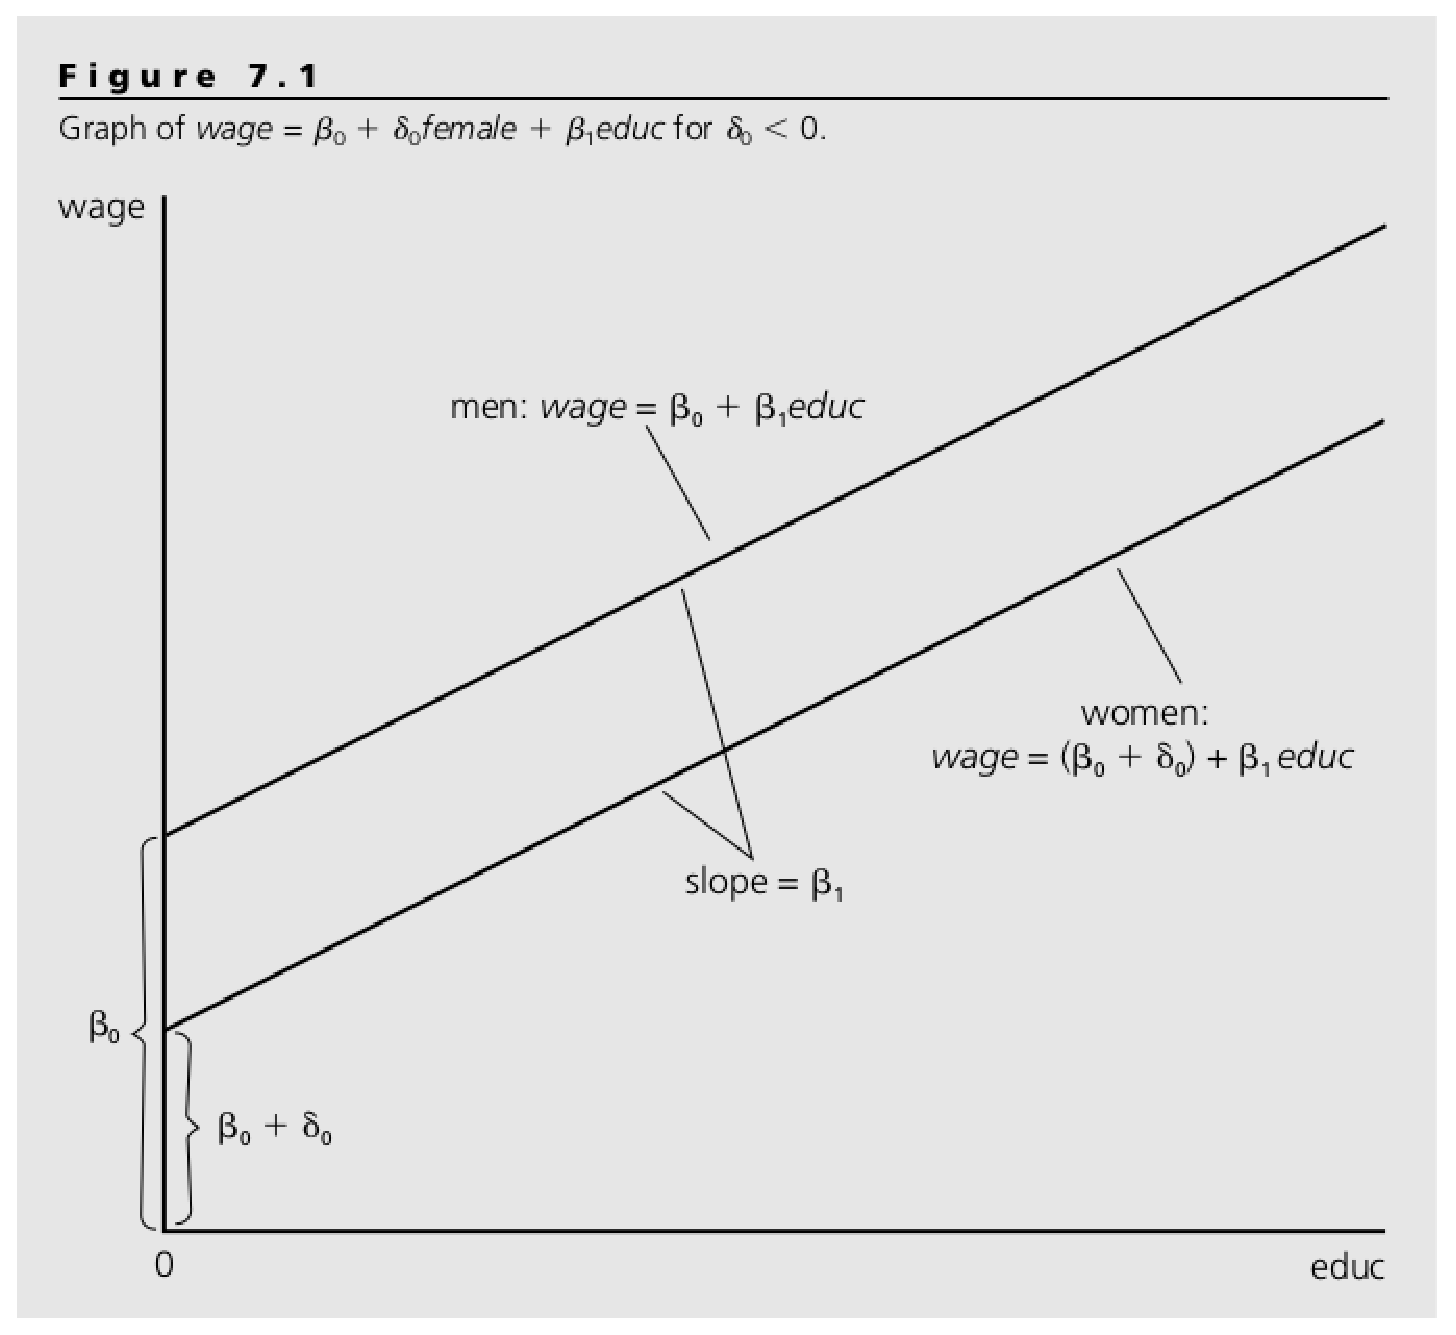
\includegraphics[scale = 0.5]{pictures/figure_7_1.eps}
\caption{Binární veličina a průsečík regresního modelu}
\label{figure_7_1}
\end{figure} 

Při používání binárních vysvětlujících veličin je třeba se 
vyvarovat tzv. pasti binární veličiny (dummy variable trap), která vede k již dříve 
diskutované dokonalé multikolinearitě. Té bychom se dopustili, 
pokud bychom regresní model (7.1) rozšířili do tvaru
\begin{equation}
wage = \beta_0 + \delta_0 female + \delta_1 male + \beta_1 educ + u,
\end{equation}
protože $female + male$ je vždy rovno jedné. Nic nám však nebrání 
tento model převést do tvaru
\begin{equation}
wage = \beta_0 + \delta_0 male + \beta_1 educ + u
\end{equation}
popř. do tvaru
\begin{equation}
wage = \delta_0 female + \delta_1 male + \beta_1 educ + u.
\end{equation}
V druhém případě jsme se vyhnuli pasti binární veličiny, 
protože jsme do modelu nezahrnuli obecný průsečík.

Testování parametru sklonu binárních veličin je stejné jako v 
případě testování sklonu standardních veličin, tj. pomocí $t$ 
testu. Aby byly závěry $t$ testu platné, musí být splněn 
předpoklad homoskedasticity, což znamená, že populační rozptyl 
příjmu mužů musí být stejný jako populační rozptyl příjmu žen.

V předchozím případě jsme uvažovali pouze dvě kategorie - muž a 
žena. Pokud však uvažujeme $n$ kategorií, je zapotřebí $n-1$ 
vysvětlujících binárních veličin.

\section{Regresní model zahrnující interakci binárních veličin}

Binární veličiny je možné mezi sebou také kombinovat. Jako 
příklad uvažujme regresní model
\begin{equation}
wage = \beta_0 + \delta_0 female + \delta_1 maried + \delta_2 female 
\cdot maried + \beta_1 educ + u.
\end{equation}
Tímto způsobem lze provést ``dekompozici'' průsečíku s ohledem na 
rodinný stav a pohlaví.

\section{Binární veličina ve funkci sklonu regresního modelu}

Binární veličiny lze snadno použít také jako ``modifikátor'' 
sklonu regresního modelu pro určitou vysvětlující veličinu. Pro 
ilustraci uvažujme model
\begin{equation}
wage = (\beta_0 + \delta_0 female) + (\beta_1 + \delta_1 female)educ + 
u
\end{equation}
resp. po roznásobení
\begin{equation}
wage = (\beta_0 + \delta_0 female) + \beta_1 educ + \delta_1 female \cdot educ + 
u,
\end{equation}
kde $\delta_0$ představuje rozdíl v průsečíku mezi muži a ženami 
a $\delta_1$ měří rozdíl v přínosu vzdělání mezi muži a 
ženami. Pokud by neexistovala mzdová diskriminaci podle pohlaví, pak 
by odhad jak $\delta_0$ tak $\delta_1$ byl statisticky 
nevýznamný.

\begin{figure}[htp]
\centering
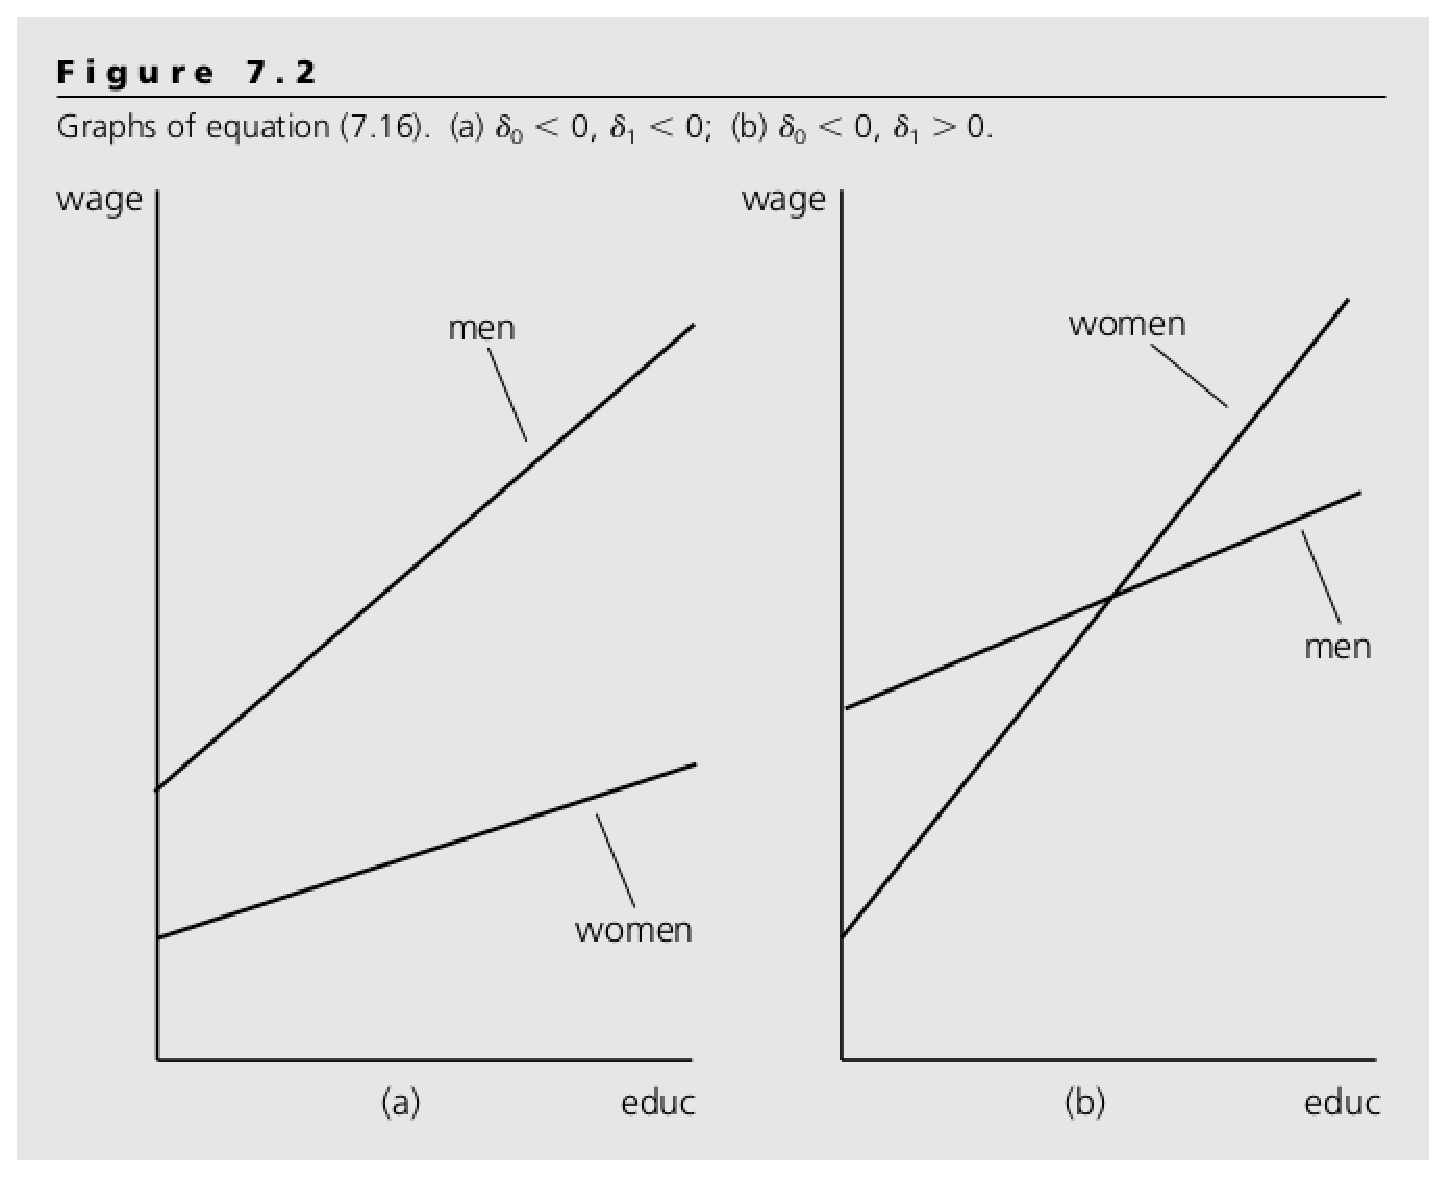
\includegraphics[scale = 0.5]{pictures/figure_7_2.eps}
\caption{Binární veličina a sklon regresního modelu}
\label{figure_7_2}
\end{figure} 

Pokud je zapotřebí testovat sdruženou významnost binárních 
veličin, tj. v našem případě nulovou hypotézu $H_0: \delta_0 = 0, 
\delta_1 = 0$, je možné použít modifikovaný $F$ test, který se 
nazývá Chowovým testem. Námi zkoumanou populaci rozdělíme na dvě 
subpopulace - na muže a ženy. Následně vypočteme $SSR_m$, $SSR_f$ 
a $SSR_P$ z odhadnutého regresního modelu pro muže
\begin{equation}
y = \beta_0^m + \beta_1^m educ + u,
\end{equation}
ženy
\begin{equation}
y = \beta_0^f + \beta_1^f educ + u
\end{equation}
a celou populaci
\begin{equation}
y = \beta_0^P + \beta_1^P educ + u.
\end{equation}
$F$ statistika je pak definována jako
\begin{equation}
F = \frac{SSR_P - (SSR_m + SSR_f)}{SSR_m + SSR_f} \frac{n - 2(k + 1)}{k 
+ 1}.
\end{equation}
Protože Chowovův test je $F$ testem, také on implicitně 
předpokládá splnění homoskedasticity, což znamená shodný rozptyl 
chybových členů pro obě subpopulace. Připomeňme, že pro účely asymptotické analýzy nemusí být 
splněn předpoklad normality.

\section{Lineární pravděpodobnostní model}

Uvažujme lineární pravděpodobnostní model (linear probability model)
\begin{equation}
y = \beta_0 + \beta_1 x_1 + ... + \beta_k x_k + u,
\end{equation}
kde $y$ má podobu binární veličiny. V tomto případě lze
\begin{equation}
E[y|x_1, ..., x_k] = \beta_0 + \beta_1 x_1 + ... + \beta_k x_k
\end{equation}
interpretovat je smyslu $P[y = 1|x_1, ..., x_k] = E[y | x_1, ..., 
x_k]$, tj. jako pravděpodobnost ``úspěchu''.

Pokud do odhadnutého regresního modelu
\begin{equation}
\hat{y} = \hat{\beta}_0 + \hat{\beta}_1 x_1 + ... + \hat{\beta}_k x_k
\end{equation}
dosadíme určité kombinace vysvětlujících veličin, může se 
stát, že predikovaná hodnota nebude spadat do intervalu nula až 
jedna, tj. bude v rozporu s jedním ze základním axiomů 
pravděpodobnosti. Tento problém lze např. vyřešit aplikací 
jednoduchého pravidla $\tilde{y}_j = 1$ pro $\hat{y}_j \ge 0.5$ a 
$\tilde{y} = 0$ pro $< 0.5$. Navzdory tomuto nedostatku je však lineární 
pravděpodobnostní model často aplikován v ekonomii. Tento model totiž 
často funguje relativně dobře pro nezávislé veličiny, jejichž 
hodnoty se nachází poblíž průměrných hodnot.

Kvůli binární povaze vysvětlované veličiny $y$ je porušen jeden 
z Gaus-Markovových předpokladů. Jestliže je $y$ binární veličinou, 
pak je její podmíněný rozptyl roven
\begin{equation}
var[y|x] = p(x)\left(1 - p(x)\right),
\end{equation}
kde $p(x)$ představuje pravděpodobnost úspěchu $p(x) = \beta_0 + 
\beta_1 x_1 + ... + \beta_k x_k$. Protože $p(x)$ je funkcí 
vysvětlujících veličin, musí být nutně porušen předpoklad 
homoskedasticity. Připomeňme, že homoskedasticita je nezbytná pro 
platnost $t$ a $F$ statistik. Proto je třeba směrodatné 
odchylky odhadnutých parametrů používat opatrně. V následující kapitole
si představíme směrodatnou odchylku, která je vzhledem k možné 
heteroskedasticitě robustní. Navíc si také ukážeme, že v praxi 
mnohdy nepředstavuje heteroskedasticita zásadní problém, a že 
standardní OLS statistiky jsou stále použitelné. 

\chapter{Heteroskedasticita}

Připomeňme, že předpoklad homoskedasticity znamená, že rozptyl 
chyby $u$ podmíněný pozorovanými hodnotami vysvětlujících veličin je 
konstantní. Tento předpoklad je nezbytný pro platnost $t$ a $F$ 
testů a pro stanovení intervalů spolehlivosti.

\section{Důsledky heteroskedasticity pro OLS}

Uvažujme regresní model
\begin{equation}
y = \beta_0 + \beta_1 x_1 + \beta_2 x_2 + ... + \beta_k x_k + u.
\end{equation}
Předpoklad homoskedasticity MLR.5 ve tvaru $var[u| x_1, ..., x_k] = 
\sigma^2$ nehraje žádnou roli tom, zda-li je OLS nestranné a 
konzistentní. Také $R^2$ není splněním či nesplněním tohoto 
předpokladu nikterak ovlivněno\footnote{Připomeňme, že $R^2 = 1 - 
\frac{\sigma^2_u}{\sigma^2_y}$. Protože $\sigma^2_u$ a 
$\sigma^2_y$ jsou nepodmíněné rozptyly, není $R^2$ ovlivněno 
splněním či nesplněním předpokladu homoskedasticity. Navíc 
$SSR/n$ je konzistentním odhadem $\sigma^2_u$ a $SST/n$ je 
konzistentním odhadem $\sigma^2_y$ bez ohledu na to, zda-li je $var[u 
| x_1, ..., x_k]$ konstantní.}.

Nicméně odhady rozptylu $var[\hat{\beta}_j]$ jsou při nesplnění 
předpokladu homoskedasticity zkreslené. Proto jsou zkreslené také 
$t$ statistiky a intervaly spolehlivosti na nich založené. Obvyklé 
OLS $t$ statistiky totiž nesledují Studentovo rozdělení a na tom se 
nic nemění ani s rostoucí velikostí náhodného výběru. Podobně 
$F$ statistika nesleduje $F$ rozdělení LM statistika nesleduje 
asymptotické chi-square rozdělení. Navíc pokud $var[u|x_1, ..., 
x_k]$ není konstantní, pak OLS není BLUE.

\section{Heteroskedasticitně robustní odhady}

\subsection{Robustní $t$ a $F$ statistika}

Jak bylo zmíněno výše, pokud není splněn předpoklad 
homoskedasticity, má to negativní dopad na $t$ a $F$ statistiky a 
intervaly spolehlivosti. Nicméně existuje způsob, jak modifikovat 
standardní směrodatné odchylky, $t$, $F$ a LM statistiky tak, aby 
byly validní i v podmínkách heteroskedasticity. Tyto postupy 
nazýváme heteroskedasticitně robustními postupy.

Uvažujme jednoduchý regresní model
\begin{equation}
y_i =\beta_0 + \beta_1 x_i + u_i,
\end{equation}
který nesplňuje předpoklad homoskedasticity, tj.
\begin{equation}
var[u_i|x_i] = \sigma^2_i.
\end{equation}
Napišme OLS odhad ve tvaru
\begin{equation}
\hat{\beta}_1 = \beta_1 + \frac{\sum_{i = 1}^n (x_i - 
\overline{x})u_i}{\sum_{i = 1}^n (x_i - \overline{x}) ^ 2}.
\end{equation}
Pokud jsou splněny předpoklady MLR.1 až MLR.4 (tj. bez 
předpokladu homoskedasticity MLR.5), pak
\begin{equation}
var[\hat{\beta}_1] = \frac{\sum_{i = 1}^n(x_i - \overline{x})^2 
\sigma^2_i}{SST^2_x},
\end{equation}
kde $SST_x = \sum_{i = 1}^n (x_i - \overline{x})^2$. Pokud $\sigma^2_i 
= \sigma^2$ pro všechna $i$, zredukuje se (8.5) na $\sigma^2/SST$. 
Jedním z možných přístupů, jak obejít skutečnost, že neznáme 
$\sigma^2_i$, je nahradit $\sigma_i$ hodnotami reziduí z odhadnutého 
regresního modelu, tj. použít
\begin{equation}
var[\hat{\beta}_1] = \frac{\sum_{i = 1}^n(x_i - \overline{x})^2 
\hat{u}^2_i}{SST^2_x}
\end{equation}
namísto (8.5). Lze dokázat, že rovnice (8.6) vynásobená velikostí 
náhodného výběru $n$ konverguje v pravděpodobnosti k $\frac{E[(x_i 
- \mu_x)^2 u_i^2]}{\left(\sigma_x^2\right)}$, což je 
pravděpodobnostní limit (8.6) krát $n$. Zákon velkých čísel a 
centrální limitní věta hrají v této konvergenci klíčovou roli.

V případě obecného regresního modelu
\begin{equation}
y = \beta_0 + \beta_1 x_1 + ... + \beta_k x_k + u
\end{equation}
při splnění předpokladů MLR.1 až MLR.4 platí
\begin{equation}
\hat{var}[\hat{\beta}_j] = \frac{\sum_{i = 1}^n 
\hat{r}_{ij}^2 \hat{u}^2_i}{SSR_j^2},
\end{equation}
kde $\hat{r}_{ij}$ je $i$-té reziduum z regrese $x_j$ na zbývající 
vysvětlující veličiny a $SSR_j$ je součet čtverců reziduí z 
této regrese. Někdy je (8.8) ještě vynásobeno $\frac{n}{n - k - 
1}$ z titulu korekce na počet stupňů volnosti\footnote{Důvodem 
této opravy je skutečnost, že pokud by $\hat{u}_i$ bylo konstantní, 
získali bychom klasickou OLS standardní odchylku.}. Druhou odmocninu z (8.8) 
pak nazýváme robustní směrodatnou odchylkou. Robustní směrodatné odchylky bývají obvykle větší než klasické OLS 
směrodatné odchylky, avšak není to pravidlo.

Robustní $t$ statistiku 
definujeme jako
\begin{equation}
t = \frac{\textit{odhad - hypotetická hodnota}}{\textit{robustní směrodatná 
odchylka}}.
\end{equation}
Jestliže je splněn předpoklad homoskedasticity a chyby regresního modelu sledují normální 
rozdělení, pak klasická $t$ statistika sleduje Studentovo rozdělení bez ohledu na velikost 
náhodného výběru. Naproti tomu robustní směrodatná odchylka a robustní $t$ statistika jsou 
ospravedlnitelné pouze pro náhodný výběr velkého rozsahu.

Vedle robustní $t$ statistiky existuje také robustní $F$ statistika (nazývaná též robustní 
Waldovou statistikou), která je její analogií.

\subsection{Robustní LM test}

LM test je možné použít namísto $F$ testu pro sdružené testování. Pro ilustraci uvažujme 
regresní model
\begin{equation}
y = \beta_0 + \beta_1 x_1 + \beta_2 x_2 + \beta_3 x_3 + \beta_4 x_4 + \beta_5 x_5 + u
\end{equation}
a uvažujme nulovou hypotézu ve tvaru $H_0: \beta_4 = 0, ~~~ \beta_5 = 0$, což implikuje 
omezený model ve tvaru
\begin{equation}
y = \beta_0 + \beta_1 x_1 + \beta_2 x_2 + \beta_3 x_3 + u.
\end{equation}

Nejprve vypočteme rezidua $\tilde{u}$ z omezeného modelu. Následně provedeme regresi 
vysvětlujících veličin $x_4$ a $x_5$ obsažených v nulové hypotéze na vysvětlující veličiny $x_1$, 
$x_2$ a $x_3$ omezeného modelu, čímž získáme rezidua $\tilde{r}_1$ a $\tilde{r}_2$. Po té 
odhadneme regresní model
\begin{equation}
1 = \alpha_1\tilde{r}_1 \tilde{u} + \alpha_2 \tilde{r}_2 \tilde{u} + v.
\end{equation}
Robustní LM statistika je rovna $n - SSR_1$, kde $n$ představuje velikost náhodného výběru a 
$SSR_1$ je součet čtverců reziduí $\hat{v}$. Při platné nulového hypotéze sleduje tato 
statistika přibližně pravděpodobnostní rozdělení $\chi^2_q$.

Výše uvedený postup lze snadno zobecnit na libovolný vícerozměrný regresní model.

\section{Testování heteroskedasticity}

\subsection{Úvod}

Připomeňme, že heteroskedasticita znamená, že OLS odhady nejsou BLUE. Proto je vhodné 
regresní model testovat na existenci heteroskedasticity.

Problém heteroskedasticity lze v praxi 
mnohdy zmírnit tím, že na místo původní vysvětlované 
veličiny $y$ použijeme její logaritmus $\ln(y)$.

Jestliže regresní model není definován správně, tj. $E[y|x]$ je systematicky zkreslené, pak 
test na heteroskedasticitu může zamítnout nulovou hypotézu, ačkoliv je $var[y|x]$ pro 
správně definovaný model konstantní. To vedlo některé ekonomy k závěru, že testy 
heteroskedasticity lze chápat jako obecné testu správnosti definice regresního modelu. 
Nicméně pro tento účel je vhodnější aplikovat specializované testy, protože nesprávná 
definice modelu představuje zásadnější problém než samotná heteroskedasticita. 

\subsection{$F$ a LM statistika}

Uvažujme regresní model
\begin{equation}
y = \beta_0 + \beta_1 x_1 + \beta_2 x_2 + ... + \beta_k x_k + u.
\end{equation}
Definujme nulovou hypotézu za předpokladu platnosti MLR.5, tj.
\begin{equation}
H_0 : var[u | x_1, x_2, ..., x_k] = \sigma^2.
\end{equation}
Zamítnutí nulové hypotézy se zpravidla interpretuje jako přítomnost hetereskedasticity v 
regresním modelu.

Protože předpokládáme, že $u$ má nulovou podmíněnou střední hodnotu, což znamená 
$var[u|x] = E[u^2|x]$, je nulová hypotéza ekvivalentní
\begin{equation}
H_0: E[u^2|x_1, x_2, ..., x_k] = E[u^2] = \sigma^2.
\end{equation}
Jinými slovy chceme testovat, zda-li existuje vztah mezi $u^2$ (v jeho očekávané hodnotě) a 
některou z vysvětlujících veličin. Proto definujme regresní model
\begin{equation}
u^2 = \delta_0 + \delta_1 x_1 + \delta_2 x_2 + ... + \delta_k x_k + v
\end{equation}
a nulovou hypotézu
\begin{equation}
H_0: \delta_1 = \delta_2 = ... = \delta_k = 0.
\end{equation}
Nulovou hypotézu lze testovat pomocí sdružené $F$ nebo LM statistiky. Testování však 
naráží na jeden praktické problém a to, že neznáme chybu $u$. Proto namísto ní použijeme 
reziduum $\hat{u}$ a (8.16) se změní na
\begin{equation}
\hat{u}^2 = \delta_0 + \delta_1 x_1 + \delta_2 x_2 + ... + \delta_k x_k + v.
\end{equation}
Lze dokázat, že použití rezidua $\hat{u}$ namísto chyby $u$ nemá vliv na pravděpodobnostní 
rozdělení $F$ popř. LM statistiky za předpokladu dostatečně velkého výběru. Důkaz je 
však poměrně komplikovaný.

Připomeňme, že $F$ statistika je definována jako
\begin{equation}
F = \frac{\frac{R^2_{\hat{u}_2}}{k}}{\frac{1 - R^2_{\hat{u}_2}}{n - k - 1}},
\end{equation}
kde $R^2_{\hat{u}_2}$ představuje $R^2$ regresního modelu (8.18), $n$ velikost náhodného 
výběru a $k$ počet vysvětlujících veličin. Při platnosti nulové hypotézy, tj. pro 
splněný předpoklad homoskedasticity, sleduje $F$ statistika přibližně pravděpodobnostní rozdělení $F_{k, n - k - 1}$.

LM statistika je definována jako
\begin{equation}
LM = n \cdot R^2_{\hat{u}^2}
\end{equation}
a při splnění předpokladu homoskedasticity asymptoticky sleduje pravděpodobnostní rozdělení 
$\chi^2_k$. LM verze testu je zpravidla nazývána Breusch-Paganovým testem heteroskedasticity.

Jestliže máme podezření, že heteroskedasticita je způsobena pouze některými 
vysvětlujícími veličinami, lze $F$ popř. LM statistiku snadno modifikovat tak, že do (8.18) 
zahrneme pouze tyto veličiny a parametr $k$ snížíme o vyloučené vysvětlující veličiny.

\subsection{Whitův test heteroskedasticity}

Původní předpoklad homoskedasticity, tj. $var[u|x_1, ..., x_k] = \sigma^2$, lze nahradit 
slabším předpokladem, že druhá mocnina chyby $u$ je nekorelovaná se všemi nezávislými 
veličinami $x_i$. Oproti původní verzi testu jsou do (8.18) přidány také druhé mocniny a vzájemné násobky 
vysvětlujících veličin. Pro ilustraci uvažujme regresní model se třemi vysvětlujícími 
proměnnými. Pak má ekvivalent (8.18) podobu
\begin{multline}
\hat{u}^2 = \delta_0 + \delta_1 x_1 + \delta_2 x_2 + \delta_3 x_3 + \delta_4 x_1^2 + \delta_5 x_2^2 
+ \delta_6 x_3^2 \\ + \delta_7 x_1 x_2 + \delta_8 x_1 x_3 + \delta_9 x_2 x_3 + v
\end{multline}
Testování nulové hypotézy
\begin{equation}
H_0: \delta_1 = \delta_2 = \delta_3 = \delta_4 = \delta_5 = \delta_6 = \delta_7 = 0
\end{equation}
pomocí $F$ popř. LM statistiky pak nazýváme Whitovým testem heteroskedasticity.

Zjevnou nevýhodou této podoby Whitova testu je zcela zřejmě velký počet testovaných 
parametrů. Při zachování původní myšlenky lze Whitův test upravit do podoby
\begin{equation}
\hat{u}^2 = \delta_0 + \delta_1 \hat{y} + \delta_2 \hat{y}^2 + v,
\end{equation}
kde $\hat{y}$ představuje odhadnuté hodnoty původního regresní modelu, tj.
\begin{equation}
\hat{y}_i = \hat{\beta}_0 + \hat{\beta}_1 x_{i1} + \hat{\beta}_2 x_{i2} + ... + \hat{\beta}_k 
x_{ik}.
\end{equation}
Odhad $\hat{y}$ používáme, protože je, na rozdíl od pozorovaných hodnot $y$, funkcí 
nezávislých proměnných. Pokud bychom namísto $\hat{y}$ použili $y$, nebyl by test validní.

Pro testování nulové hypotézy $H_0: \delta_1 = \delta_2 = 0$ v (8.23) lze použít jak $F$ tak 
LM statistiku s parametrem $k = 2$ bez ohledu na počet vysvětlujících proměnných.

\section{Odhad metodou nejmenších čtverců}

\subsection{Heteroskedasticita jako funkce vysvětlujících veličin}

Uvažujme
\begin{equation}
var[u|x] = \sigma^2 h(x),
\end{equation}
kde $h(x)$ je funkcí vysvětlujících veličin. Protože rozptyl musí být kladný, musí platit 
$h(x) > 0$.

Při náhodném výběru z populace můžeme psát $\sigma_i^2 = var[u_i |x_i] = \sigma^2 h(x_i) = 
\sigma^2 h_i$. Pro ilustraci předpokládejme regresní model, který vysvětluje vztah mezi úrovní 
úspor a výší příjmu.
\begin{equation}
sav_i = \beta_0 + \beta_1 inc_i + u_i
\end{equation}
\begin{equation}
var[u_i | inc_i] = \sigma^2 inc_i
\end{equation}
Rozptyl chyby v tomto regresním modelu je proporcionální výši příjmu.

Uvažujme obecný regresní model
\begin{equation}
y_i = \beta_0 + \beta_1 x_{i1} + \beta_2 x_{i2} + ... + \beta_k x_{ik} + u_i,
\end{equation}
který je zatížený heteroskedasticitou. Protože $h_i$ je pouze funkcí $x_i$, má 
$\frac{u_i}{\sqrt{h_i}}$ nulovou podmíněnou střední hodnotu vzhledem $x_i$. Dále, protože 
$var[u_i|x_i] = E[u_i^2 | x_i] = \sigma^2 h_i$, je podmíněný rozptyl $\frac{u_i}{\sqrt{h_i}}$ 
vzhledem k $x_i$ roven $\sigma^2$.
\begin{equation}
E\left[\left(\frac{u_i}{\sqrt{h_i}}\right)^2\right] = \frac{E[u_i^2]}{h_i} = \frac{\sigma^2 
h_i}{h_i} = \sigma^2
\end{equation}
Proto lze (8.28) podělit $\sqrt{h_i}$, čímž získáme
\begin{equation}
\frac{y_i}{\sqrt{h_i}} = \beta_0 \frac{1}{\sqrt{h_i}} + \beta_1 \frac{x_{i1}}{\sqrt{h_i}} + \beta_2 
\frac{x_{i2}}{\sqrt{h_i}} + ... + \beta_k \frac{x_{ik}}{\sqrt{h_i}} + u_i \frac{1}{\sqrt{h_i}}
\end{equation}
neboli
\begin{equation}
y^*_i = \beta_0 x^*_{i0} + \beta_1 x^*_{i1} + ... + \beta_k x^*_{ik} + u^*_i
\end{equation}
a tím odstranit z modelu heteroskedasticitu.

Odhady parametrů na základě (8.31) jsou příklady tzv. obecných odhadů 
metodou nejmenších čtverců (generalized least squares estimators - GLS estimators). GLS odhady 
pro korekci heteroskedasticity jsou též nazývány odhady metodou vážených nejmenších 
čtverců (weighted least squares estimators - WLS estimators)\footnote{OLS lze chápat jako 
zvláštní příklad WLS odhadů, které dává stejnou váhu všem pozorováním.}. Protože 
jsme z modelu (8.31) odstranili heteroskedasticitu, jsou tyto odhady, na rozdíl od odhadů na 
základě modelu (8.28), nejlepšími nezkreslenými lineárními odhady.

Problém výše uvedeného přístupu je ten, že skutečné váhy neznáme a jejich volba je do 
značné míry arbitrární.

\subsection{Dosažitelné GLS odhady}

V řadě případů můžeme zkonstruovat model funkce $h$ a použít data k odhadu jeho 
parametrů, tj. pro každé $h_i$ získat jeho odhad $\hat{h}_i$ - hovoříme o tzv. 
dosažitelných GLS odhadech.

Jako příklad takovéhoto modelu uvažujme model\footnote{Připomeňme, že uvažovaná funkce modelu musí být vždy kladná.}
\begin{equation}
var[u|x] = \sigma^2 e^{\delta_0 + \delta_1 x_1 + \delta_2 x_2 + ... + \delta_k x_k}.
\end{equation}
Za předpokladu (8.32) můžeme psát
\begin{equation}
u^2 = \sigma^2 e^{(\delta_0 + \delta_1 x_1 + \delta_2 x_2 + ... + \delta_k x_k)v},
\end{equation}
kde $v$ má podmíněný průměr vzhledem k $x = (x_1, x_2, ..., x_k)$ roven jedné. Jestliže 
předpokládáme, že $v$ je nezávislé na $x$, pak můžeme výše uvedený model upravit do tvaru
\begin{equation}
\ln(u^2) = \alpha_0 + \delta_1 x_1 + \delta_2 x_2 + ... + \delta_k x_k + e,
\end{equation}
kde $e$ má nulovou střední hodnotu a je nezávislé na $x$. Průsečík $\alpha_0$ je různý od 
původního průsečíku $\delta_0$, ale to není pro implementaci WLS důležité. Protože (8.33) 
splňuje Gauss-Markovovy předpoklady, můžeme získat nezkreslené odhady $\delta_i$ pomocí OLS. 
Protože v praxi neznáme chybu $u$, nahradíme ji opět reziduem $\hat{u}$. Náš regresní model 
bude tedy mít podobu
\begin{equation}
\ln(\hat{u}^2) = \alpha_0 + \delta_1 x_1 + \delta_2 x_2 + ... + \delta_k x_k + e.
\end{equation}
Z této regrese potřebujeme predikované hodnoty $E[\ln(\hat{u_i}^2) | x_i] = \hat{g_i}$. 
Odhad funkce $h_i$ je pak definován jako
\begin{equation}
\hat{h}_i = e^{\hat{g_i}}.
\end{equation}

Pokud bychom mohli namísto $\hat{h}_i$ použít $h_i$, byly by naše odhady nezkreslené. 
Protože však odhadujeme $h_i$ pomocí stejných dat, jaká následně použijeme pro odhad 
parametrů původního regresního modelu, jsou naše dosažitelné GLS odhady zkreslené. Tyto 
odhady jsou však konzistentní a asymptoticky efektivnější než prosté OLS odhady. Důkaz 
tohoto tvrzení je však komplikovaný.

Další užitečnou alternativou pro odhad $h_i$ je nahrazení nezávislých proměnných v (8.35) 
hodnotami predikovanými pomocí klasické OLS, tj.
\begin{equation}
\ln(\hat{u}^2) = \alpha_0 + \delta_1 \hat{y} + \delta_2 \hat{y}^2.
\end{equation}
Získání odhadu $\hat{h}_i$ je stejné jako v předchozím případě.

Při aplikaci $F$ testu musíme použít stejné váhy pro omezený a neomezený model. Nejprve 
tedy odhadneme neomezený model s pomocí OLS. Jakmile máme k dispozici váhy, můžeme je 
použít k odhadu omezeného modelu. $F$ statistiku pak vypočteme obvyklým způsobem.

OLS a WLS odhady se mohou různit. Pokud OLS a WLS vedou k statisticky významným odhadům, 
které se liší znaménkem nebo je rozdíl v odhadech příliš velký, je to zpravidla důsledkem 
porušení některého z dalších Gauss-Markovových předpokladů zejména pak předpokladu 
nulové podmíněné střední hodnoty chyby regresního modelu (MLR.4). Jestliže totiž $E[y|x]  
\ne \beta_0 + \beta_1 x_1 + ... + \beta_k x_k$, pak mají OLS a WLS odhady rozdílné očekávané hodnoty 
a pravděpodobnostní rozdělení. Aby WLS bylo konzistentní v $\beta_j$ nestačí, aby $u$ bylo 
nekorelované s každým jednotlivým $x_j$ - je zapotřebí splnění silnějšího předpokladu 
MLR.4 v lineárním modelu MLR.1. Významný rozdíl mezi OLS a WLS odhady tak indikuje problémy s 
funkční specifikací $E[y|x]$.

\subsection{Chybná funkce $h(x)$}

Jaké jsou vlastnosti WLS, jestliže je funkce $h(x)$ chybně specifikována, tj. pokud $var[y|x] 
\ne \sigma^2 h(x)$?

Jestliže $E[u|x] = 0$, pak libovolná funkce $h(x)$ je nekorelovaná s $u$, a proto je také 
$\frac{u}{\sqrt{h(x)}}$ nekorelované s vysvětlujícími veličinami $\frac{x_j}{\sqrt{h(x)}}$ pro 
libovolné $h(x) > 0$. Z tohoto důvodu můžeme velké rozdíly mezi OLS a WLS 
odhady chápat jako indikaci chybné specifikace regresního modelu. Pokud odhadneme parametry $\hat{\delta}$ 
ve funkci $h(x, \hat{\delta})$, nemůžeme již tvrdit, že WLS odhady jsou nezkreslené. Tyto 
odhady však budou konzistentní a to bez ohledu na to, zda byla funkce $h(x)$ specifikována 
správně či nikoliv.

V případě chybně specifikované funkce $h(x)$ však nejsou směrodatné odchylky a $t$ popř. 
$F$ statistiky WLS odhadů platné a to ani v případě výběrů velkého rozsahu. Naštěstí, 
stejně jako v případě robustních OLS odhadů, lze také pro WLS odhady, které připouštějí 
chybnou specifikaci funkce $h(x)$. Jestliže má transformovaný regresní model tvar
\begin{equation}
\frac{y_i}{\sqrt{h_i}} = \beta_0 \frac{1}{\sqrt{h_i}} + \beta_1 \frac{x_{i1}}{\sqrt{h_i}} + ... + 
\beta_k \frac{x_{ik}}{\sqrt{h_i}} + \frac{u_i}{\sqrt{h_i}},
\end{equation}
přičemž $var[u_j | x_j] \ne \sigma^2 h_j$. Vážená chyba $\frac{u_i}{\sqrt{h_i}}$ je tedy 
heteroskedastická. Nicméně po odhadu parametrů (8.38) pomocí OLS lze pro výpočet jejich intervalů 
spolehlivosti a testování hypotéz použít robustní směrodatné odchylky stejně jako v případě OLS.

I když použijeme obecné formy typu (8.32) pro odhad funkce $h(x)$, nemáme jistotu správné 
specifikace. Proto je vždy vhodné vždy používat robustní směrodatné odchylky.

Moderní kritika WLS spočívá v argumentu, že pokud není funkce $h(x)$ správně 
specifikována, nemáme jistotu, že WLS odhady budou efektivnější než klasické OLS odhady. 
Nicméně v případě silné heteroskedasticity je zpravidla lepší použít špatně 
specifikovanou funkci $h(x)$, než tento problém zcela ignorovat.

\subsection{Predikce a heteroskedasticita}

Intervaly spolehlivosti pro predikované hodnoty závisí přímo na povaze $var[y|x]$. 
Předpokládejme, že jsou splněny všechny CLM předpoklady s výjimkou předpokladu 
homoskedasticity (MLR.5), který je nahrazen (8.25).

Směrodatnou odchylku $se(\hat{y}^0)$ lze získat stejným způsobem jako v kapitole 6.4 pouze s 
tím rozdílem, že namísto OLS použijeme WLS. Dále potřebujeme odhadnout směrodatnou odchylku 
pro $u^0$, které představuje tu část $y^0$, která není podchycena vysvětlujícími 
veličinami. Protože však předpokládáme $var[u^0|x = x^0] = \sigma^2 h(x^0)$, pak $se(u^0) = 
\hat{\sigma} \sqrt{h(x^0)}$, kde $\hat{\sigma}$ je směrodatná odchylka regrese z WLS odhadu. 95\% 
interval spolehlivosti je tak
\begin{equation}
\hat{y}^0 \pm t_{0.025} se(\hat{e}^0),
\end{equation}
kde $se(\hat{e}^0) = \sqrt{\left(se(\hat{y}^0)\right)^2 + \left(se(\hat{x}^0)\right)^2}$. Tento 
interval spolehlivosti je přesný pouze v případě, že nemusíme odhadnout funkci $h(x)$. 
Jestliže musíme odhadnout parametry jako ve funkční specifikaci (8.32), pak nelze získat 
přesný interval spolehlivosti. Zohlednění případné chyby v odhadu $\hat{\beta}_j$ a $\hat{\delta}_j$ je 
však velmi složité. Proto v praxi v (8.39) jednoduše nahradíme $h(x^0)$ jejím odhadem 
$\hat{h}(x^0)$. Pokud se rozhodneme ignorovat chybu odhadu parametru, můžeme jednoduše vypustit 
$se(\hat{y}^0)$ z $se(\hat{e}^0)$\footnote{Připomeňme, že $se(\hat{y}^0)$ konverguje k nule 
rychlostí $\frac{1}{\sqrt{n}}$, zatímco $se(\hat{u}^0)$ zůstává přibližně konstantní.}.

\subsubsection{Ilustrativní příklad}

Pro ilustraci uvažujme regresní model
\begin{equation}
\ln(y) = \beta_0 + \beta_1 x_1 + ... + \beta_k x_k + u,
\end{equation}
kde $u$ je heteroskedastické. Předpokládejme, že známe formu heteroskedasticity a že 
je splněna podmínka normality, tj.
\begin{equation}
u | x_1, x_2, ..., x_k \sim N(0, e^{\delta_0 + \delta_1 x_1 + ... + \delta_k x_k}).
\end{equation}

Protože $\ln(y)$ pro dané $x = (x_1, X_2, ..., x_k)$ sleduje normální rozdělení se střední 
hodnotou $\beta_0 + x \beta$ a rozptyl $e^{\delta_0 + x \delta}$, platí
\begin{equation}
E[y|x] = e^{\beta_0 + x \beta + \sigma^2 e^{(\delta_0 + x \delta})/2}.
\end{equation}

Nejprve odhadneme $\beta_j$ a $\delta_j$ s pomocí WLS z (8.40). Po 
získání reziduí pomocí OLS provedeme regresi (8.35) s cílem získat predikované hodnoty
\begin{equation}
\hat{g}_i = \hat{\alpha}_0 + \hat{\delta}_1 x_{i1} + ... + \hat{\delta}_k x_{ik},
\end{equation}
které použijeme pro odhad $\hat{h}_i$ pomocí (8.36). S pomocí $\hat{h}_i$ pak získáme WLS 
odhady $\hat{\beta_j}$ a $\hat{\sigma}^2$.

Dále získáme predikované hodnoty
\begin{equation}
\hat{y}_i = e^{\widehat{\ln(y_i)} + \hat{\sigma}^2 \hat{h}_i / 2}.
\end{equation}
Tyto predikované hodnoty můžeme použít pro získání $R^2$ tak, jak je popsáno v kapitole 
6.4, tj. použít druhou mocninu korelačního koeficientu mezi $y_i$ a $\hat{y}_i$.

Pro libovolné 
hodnoty vysvětlujících veličin $x^0$ pak lze získat predikci pomocí
\begin{equation}
\hat{E}[y | x = x^0] = e^{\hat{\beta}_0 + \hat{\beta} x^0 + \hat{\sigma}^2 e^{(\hat{\alpha}_0 + 
\hat{\delta}x^0) / 2}},
\end{equation}
kde $\hat{\beta}_j$ představuje WLS odhad a $\hat{\alpha}_0$ a $\hat{\delta}_j$ jsou odhady 
parametrů v (8.43).

Získání správné směrodatné odchylky pro predikci z (8.44) analyticky je
poměrně komplikované, nicméně ji lze poměrně snadno získat metodou opakovaného výběru, 
která je popsána v kapitole 6.A.

Přibližný 95\% interval spolehlivosti pro výběry velkého rozsahu je definován rozmezím 
$e^{-1.96 \hat{\sigma} \sqrt{\hat{h} x^0}} e^{\hat{\beta}_0 + \hat{\beta}x^0}$ až $e^{1.96 
\hat{\sigma} \sqrt{\hat{h} x^0}} e^{\hat{\beta}_0 + \hat{\beta}x^0}$, kde $\hat{h}(x^0)$ je odhad 
funkce $h(x)$ v bodě $x^0$, tj. $\hat{h}(x^0) = e^{\hat{\alpha}_0 + \hat{\beta}_1 x^0_1 + ... + 
\hat{\delta}_k x^0_k}$.

\section{Lineární pravděpodobnostní model}

V případě, že má vysvětlovaná veličina charakter binární veličiny, musí model obsahovat 
heteroskedasticitu, pokud nejsou všechny parametry sklonu rovny nule.

Nejjednodušším způsobem, jak se vypořádat s heteroskedasticitou v lineární 
pravděpodobnostním modelu (linear probability model - LPM) je použít OLS odhady a 
robustní směrodatnou odchylku při testování hypotéz a konstrukci konfidenčních intervalů. 
Tento přístup však ignoruje skutečnost, že známe formu heteroskedasticity pro LPM. Odhad LPM 
pomocí OLS je však poměrně snadný a v praxi velmi často vede k uspokojivým výsledkům. To 
nám však nebrání nastínit postup, jakým lze heteroskedasticitu z modelu odstranit.

Obecně platí, že OLS odhady jsou v případě LPM neefektivní. Připomeňme, že podmíněný 
rozptyl vysvětlované veličiny $y$ je pro LPM definován jako
\begin{equation}
var[y | x] = p(x)[1 - p(x)],
\end{equation}
kde
\begin{equation}
p(x) = \beta_0 + \beta_1 x_1 + ... + \beta_k x_k.
\end{equation}
Pravděpodobnost $p(x)$ tak zcela zřejmě závisí na parametrech $\beta_j$, které jsme schopni 
odhadnout pomocí OLS. Pro každé $i$-té pozorování je tak $var[y_i | x_i]$ odhadnut pomocí
\begin{equation}
\hat{h}_i = \hat{y}_i (1 - \hat{y}_i),
\end{equation}
kde predikované hodnoty $\hat{y}_i$ nemusí vždy spadat do jednotkového intervalu. Pokud však 
$\hat{y}_i < 0$ nebo $\hat{y}_i > 1$, pak $\hat{h}_i$ v (8.48) bude nulové nebo záporné. 
Protože v rámci WLS používáme váhy $\frac{1}{\sqrt{\hat{h}_i}}$, musí být $\hat{h}_i$ 
kladné. Triviální řešením tohoto problému je např. nastavit $\hat{y}_i = 0.01$ pokud 
$\hat{y}_i < 0$ a $\hat{y}_i = 0.99$ pokud $\hat{y}_i > 1$. Pokud je však příliš mnoho hodnot 
mimo jednotkový interval, je pravděpodobně vhodnější použít klasické OLS.

\chapter{Specifikace modelu a datové problémy}

\section{Chybná specifikace modelu}

Nejčastější formou chybné specifikace regresního modelu je opomenutí relevantní nezávislé veličiny. Nicméně se nejedná o jedinou možnou formu chybné specifikace modelu. Další možností je začlenění nezávislé veličiny v nesprávné podobě, kdy např. namísto $log(x_{tj})$ do modelu přidáme $x_{tj}$.

Chybná specifikace modelu může mít závažné důsledky - typickým problémem je zkreslenost a nekonzistence odhadnutých parametrů regresního modelu.

Pro detekci chybné specifikace modelu lze použít $F$ test pro sdružené testování hypotéz, který jsme představili již dříve. V praxi se např. poměrně často do regresního modelu přidává kvadratický člen pro nejvýznamnější nezávislé proměnné a model se pak následně testuje na sdruženou významnost vysvětlujících veličin.

V praxi je mnohdy velmi obtížné zjistit příčinu chybné specifikace modelu, nicméně v řadě případů tento problém vyřeší aplikace logaritmu na vysvětlující veličiny a zavedení kvadratických členů. To však v řadě případů může snížit interpretovatelnost daného regresního modelu.

\subsection{RESET a obecný test chybné specifikace modelu}

Ramsey (1969) navrhl tzv. test chybné specifikace chybového členu [regression specification error test (RESET)]. Pro ilustraci uvažujme model
\begin{equation}
y = \beta_0 + \beta_1 x_1 + ... + \beta_k x_k + u,
\end{equation}
který splňuje MLR.4. To implikuje, že žádná z nelineárních funkcí nezávislých veličin by neměla být po přidání do modelu (9.1) shledána jako statisticky signifikantní. RESET test přidává do modelu polynomy nezávislých veličin $\hat{y}$ odhadnutých z původního modelu. Neexistuje žádné exaktní pravidlo pro řád polynomů, které by měly být zahrnuty, nicméně v praxi se nejčastěji přidávají polynomy druhého a třetího řádu. Model (9.1) se tak změní na
\begin{equation}
y = \beta_0 + \beta_1 x_1 + ... + \beta_k x_k + \delta_1 \hat{y}^2 + \delta_2 \hat{y}^3.
\end{equation}
Je důležité si uvědomit, že $\hat{y}^2$ a $\hat{y}^3$ hrají ve výše uvedeném modelu roli nelineárních funkcí nezávislých proměnných $x_j$.

Nulová hypotéza RESET testu je, že model (9.1) je správně specifikován, tj. pomocí $F$ statistiky testujeme $H_0: \delta_1 = 0, \delta_2 = 0$. Statisticky signifikantní $F$ statistika pak indikuje problémy se specifikací modelu. Pravděpodobnostní rozdělení $F$ statistiky pro náhodné výběry velkého rozsahu při splnění nulové hypotézy (a Gauss-Markovových předpokladů) přibližně sleduje $F_{2, n - k -3}$, kde $n - k - 3$ představuje počet stupňů volnosti modelu (9.2). Tento test lze taktéž učinit heteroskedasticitně robustním tak, jak jsme diskutovali v kapitole 8.

Hlavní nevýhodou RESET testu je, že nám neřekne, jak model modifikovat, pokud je nulová hypotéza zamítnuta.

\subsection{Nevnořené modely}

Předpokládejme, že chceme testovat model
\begin{equation}
y = \beta_0 + \beta_1 x_1 + \beta_2 x_2 + u
\end{equation}
proti modelu
\begin{equation}
y = \beta_0 + \beta_1 \log(x_1) + \beta_2 \log(x_2) + u.
\end{equation}
Bohužel se jedná o tzv. nevnořené modely (nonnested models), a proto nelze jednoduše použít $F$ test. Namísto původních dvou modelů uvažujme model
\begin{equation}
y = \delta_0 + \delta_1 x_1 + \delta_2 x_2 + \delta_3 \log(x_1) + \delta_4 \log(x_2) + u.
\end{equation}
Můžeme testovat $H_0: \delta_3 = 0, \delta_4 = 0$ jako test modelu (9.3) popř. $H_0: \delta_1 = 0, \delta_2 = 0$ jako test modelu (9.4).

Existuje však ještě jedna možnost. Jestliže je model (9.3) pravdivý, pak by $\hat{y}$ odhadnuté na základě modelu (9.4) měly být v modelu (9.3) statisticky nevýznamné. Tento test se nazývá Davidson-MacKinnonovým testem a je založen na $t$ statistice $\hat{y}$ modelu
\begin{equation}
y = \beta_0 + \beta_1 x_1 + \beta_2 x_2 \theta_1 \hat{y} + error,
\end{equation}
kde $\hat{y}$ je odhadnuto z modelu (9.4). Statisticky signifikantní $t$ statistika je důkazem proti modelu (9.3). Test lze snadno modifikovat tak, abychom pomocí $\hat{y}$ z modelu (9.3) testovali validitu modelu (9.4). Davidson-MacKinnonův test může zamítnout oba nebo také žádný z modelů; v tomto případě nemá test jasného vítěze. Je důležité si také uvědomit, že pokud test zamítne platnost modelu (9.3), neznamená to automatickou platnost modelu (9.4). David-MacKinnonův test lze použít pouze v případě, kdy uvažované modely mají shodnout závislou veličinu\footnote{To znamená, že test nelze aplikovat např. v situaci, kdy závislá veličina v jednom z modelů má tvar $y$ a v druhém $\log(y)$.} a jsou vystavěny na totožných nezávislých veličinách. Existují i zobecněné testy, které splnění těchto podmínek nevyžadují, ty však přesahují záběr naší knihy.

\section{Proxy veličiny}

Jedním z nejčastějších případů chybné specifikace modelu je opomenutí relevantní vysvětlující veličiny z důvodu obtížné nebo dokonce nemožného sběru dat. Jako příklad uvažujme regresní model, který vysvětluje vývoj mezd a který zahrnuje schopnost daného jedince \textit{abil} jako jednu z vysvětlujících veličin.
\begin{equation}
log(wage) = \beta_0 + \beta_1 educ + \beta_2 exper + \beta_3 abil + u
\end{equation}
Je zřejmé, že vysvětlující veličina \textit{abil} se velice obtížně kvantifikuje. Pokud bychom ji však z modelu vypustili, bude odhad parametru $\beta_1$ zkreslen a to z titulu korelace mezi \textit{educ} a \textit{abil}. Podobnou argumentaci lze aplikovat také v případě parametru $\beta_2$. Řešením tohoto problému je namísto \textit{abil} použít proxy nezávislou veličinu jako např. IQ daného jedince.

Hlavní myšlenky konceptu proxy nezávislé veličiny lze ilustrovat pomocí modelu
\begin{equation}
y = \beta_0 + \beta_1 x_1 + \beta_2 x_2 + \beta_3 x_3^* + u,
\end{equation}
kde $x_3$ nelze kvantifikovat, a proto namísto ní použijeme proxy $x_3^*$. Předpokládejme, že vztah mezi $x_3$ a $x_3^*$ lze popsat pomocí 
\begin{equation}
x_3^* = \delta_0 + \delta_3 x_3 + v_3.
\end{equation}
Protože $x_3$ a $x_3^*$ nejsou identická, lze použít poučku pro zkreslení z titulu opomenutí relevantní veličiny. Abychom substitucí $x_3^*$ za $x_3$ získali konzistentní odhady $\beta_1$ a $\beta_2$, musí být splněny následující předpoklady.
\begin{enumerate}
\item Chyba $u$ z modelu (9.8) není korelována s $x_1$, $x_2$ ani $x_3^*$. Toto jsou standardní předpoklady regresního modelu. Navíc však $u$ nesmí být korelováno ani s původní nezávislou veličinou $x_3$. Tento předpoklad nám říká, že pokud jsou do modelu začleněny $x_1$, $x_2$ a $x_3^*$, je $x_3$ z pohledu modelu irelevantní.
\item Chyba $v_3$ je nekorelovaná s $x_1$, $x_2$ a $x_3$. Tento předpoklad vyžaduje, aby $x_3^*$ byla ``dobrou'' proxy veličinou pro $x_3$, což je zřejmé z podmíněné hodnoty $x_3^*$.
\begin{equation}
E[x_3^* | x_1, x_2, x_3] = E[x_3^* | x_3] = \delta_0 + \delta_3 x_3
\end{equation}
Tato rovnice nám říká, že jakmile je zafixováno $x_3$, je střední hodnota $x_3^*$ nezávislá na $x_1$ a $x_2$.
\end{enumerate}
Jestliže dosadíme (9.9) do (9.8), získáme
\begin{equation}
y = (\beta_0 + \beta_3 \delta_0) + \beta_1 x_1 + \beta_2 x_2 + \beta_3 \delta_3 x_3 + u + \beta_3 v_3,
\end{equation}
což lze dále upravit na
\begin{equation}
y = \alpha_0 + \beta_1 x_1 + \beta_2 x_2 + \alpha_3 x_3 + e.
\end{equation}
Aplikací OLS na (9.12) sice nezískáme nezkreslené odhady parametrů $\beta_0$ a $\beta_3$, ale získáme nezkreslené (nebo alespoň konzistentní) odhady $\alpha_0$, $\beta_1$, $\beta_2$ a $\alpha_3$. Klíčovou výhodou tohoto postupu jsou nezkreslené odhady $\beta_1$ a $\beta_2$. Co se odhadu $\beta_3$ týče, ten je pro nás v praxi zpravidla méně zajímavý než odhad parametru $\alpha_3$.

Pokud proxy veličina nesplňuje výše uvažované předpoklady, jsou odhady regresního modelu zkreslené. Pro ilustraci uvažujme
\begin{equation}
x_3^* = \delta_0 + \delta_1 x_1 + \delta_2 x_2 + \delta_3 x_3 + v_3
\end{equation}
namísto (9.9). Substituce (9.12) do (9.8) vede k modelu
\begin{equation}
y = (\beta_0 + \beta_3 \delta_0) + (\beta_1 + \beta_3 \delta_1) x_1 + (\beta_2 + \beta_3 \delta_3) x_2 + \beta_3 \delta_3 x_3 + u + \beta_3 v_3,
\end{equation}
ze kterého plyne $plim(\hat{\beta}_1) = \beta_1 + \beta_3 \delta_1$ a $plim(\hat{\beta}_2) + \beta_2 + \beta_3 \delta_2$.\footnote{To vyplývá z toho, že chyba $u + \beta_3 v_3$ v modelu (9.14) má nulovou střední hodnotu a je nekorelovaná s $x_1$, $x_2$ a $x_3$.} Pokud $x_3^*$ není ``dobrá'' proxy veličina, jsou odhady ostatních parametrů stále zkreslené. Lze však očekávat, že toto zkreslení bude menší, než kdybychom proxy veličinu do regresního modelu nezahrnuli.

\subsection{Zpožděné proxy veličiny}

V řadě případů mohou být některé z nezávislých veličin zahrnutých do modelu korelované s opomenutou veličinou, pro kterou může být složité nalézt vhodnou proxy veličinu. Problém lze často vyřešit zahrnutím zpožděných závislých veličin. Tento koncept je vhodný např. při formulování měnové či fiskální politiky, kde zpožděné nezávislé veličiny vnášejí do modelu historickou informaci spojenou s faktorem, který je velmi obtížné konkretizovat. Jako příklad uvažujme model
\begin{equation}
hdp_t = \beta_0 + \beta_1 hdp_{t - 1} + \beta_2 unpl_t + \beta_3 unpl_{t - 1} + \beta_4 infl_t + \beta_5 infl_{t - 1}.
\end{equation}

\subsection{Odlišný pohled na vícerozměrnou regresi}

V předchozím textu jsme použili namísto vágního pojmu schopnost (\textit{abil}) proxy veličinu IQ. K této problematice však lze zaujmout také odlišný postoj. Konkrétně naším zájmem může být snaha o co nejlepší odhad mzdy daného jedince, pokud známe jeho IQ a ostatní vysvětlující veličiny. Zásadní rozdíl je ten, že se nesnažíme dobrat se modelu (9.7). Vzhledem k omezením, kterým čelíme v praxi (neznalost správného regresního modelu, neschopnost korektně kvantifikovat nezávislé veličiny), jsme se smířili s omezenou množinou vysvětlujících veličin, které máme k dispozici a s jejich pomocí se snažíme získat co nejlepší odhad mzdy.

\section{Modely s náhodným sklonem}

Uvažujme model, ve kterém se parciální efekt určité nezávislé veličiny, kterou nejsme schopni kvantifikovat, mění s jednotlivými populačními členy. Jestliže máme pouze jednu nezávislou veličinu $x$, můžeme obecnou rovnici pro náhodně vybrané pozorování definovat jako
\begin{equation}
y_i = a_i + b_i x_i,
\end{equation}
kde $a_i$ je průsečík a $b_i$ je sklon pro $i$-té pozorování. V kontextu jednoduchého regresního modelu, který jsme představili v kapitole 2, platí $b_i = \beta$ a $a_i = u_i$. Model (9.16) je někdy nazýván modelem s náhodným sklonem (random slope model), protože na parametr $b_i$ lze pohlížet jako na náhodný výběr z populace společně s daty $(x_i, y_i)$ a průsečíku $a_i$. Pokud bychom se vrátili k našemu modelu mzdy, pak by $b_i$ (ale také $a_i$) v sobě zahrnovala efekt schopnosti konkrétního jedince.

S tím, jak z populace získáme $n$ náhodných pozorování, získáme také $n$ parametrů $b_i$ a $a_i$. Je zřejmé, že nejsme schopni odhadnout každé jednotlivé $b_i$ a $a_i$, nicméně můžeme odhadnout průměrný sklon a průsečík napříč celou populací. Proto definujeme $\alpha = E[a_i]$ a $\beta = E[b_i]$. $\beta$ tak nazýváme průměrným parciálním efektem [average partial effect (APE)].

Jestliže definujeme $a_i = \alpha + c_i$ a $b_i = \beta + d_i$, pak lze na $c_i$ a $d_i$ pohlížet jako na specifickou odchylku daného jedince od populačního průměru. Dle definice platí $E[c_i] = 0$ a $E[d_i] = 0$. Dosazením do (9.16) pak získáme
\begin{equation}
y_i = \alpha + \beta_i x_i + c_i + d_i x_i \equiv \alpha + \beta x_i + u_i,
\end{equation}
kde $u_i = c_i + d_i x_i$. Jinými slovy, náhodný člen $u_i$ zahrnuje interakci mezi veličinou $d_i$, kterou nejsme schopni kvantifikovat, a vysvětlující veličinou $x_i$.

Pokud je splněn předpoklad $E[u_i | x_i] = 0$, pak jsou OLS odhady nezkreslené. Jestliže $u_i = c_i + d_i x_i$, je dostatečné $E[c_i|x_i] E[c_i] = 0$ a $E[d_i|x_i] = E[d_i] = 0$. Pak totiž platí
\begin{equation}
E[a_i|x_i] = E[a_i] ~~~ E[b_i|x_i] = E[b_i].
\end{equation}
Jestliže tedy připustíme myšlenku ``individuálního'' sklonu pro jednotlivé členy populace, pak OLS konzistentně odhaduje populační průměr tohoto sklonu.

Jestliže $var[c_i|x_i] = \sigma_c^2$, $var[d_i|x_i] \sigma_d^2$ a $cov[c_i, d_i, | x_i] = 0$, pak
\begin{equation}
var[u_i | x_i] = \sigma_c^2 + \sigma_d^2 x_i^2,
\end{equation}
a proto chybový člen v (9.17) musí vykazovat známky heteroskedasticity s výjimkou, kdy $\sigma_d^2 = 0$, což implikuje $b_i = \beta$ pro všechna $i$. Někteří autoři tak vnímají heteroskedasticitu jako důsledek náhodného sklonu. Nicméně v praxi nejsme schopni rozlišit mezi regresním modelem s náhodným sklonem a modelem s konstantním sklonem a heteroskedasticitou v $a_i$.

V případě vícerozměrného regresního modelu je postup analogický. Uvažujme model
\begin{equation}
y_i = a_i + b_{i1} x_{i1} + b_{i2} x_{i2} + ... + b_{ik}x_{ik}.
\end{equation}
Pokud $a_i = \alpha + c_i$ a $b_{ij} = \beta_j + d_{ij}$, pak lze tento model zapsat jako
\begin{equation}
y_i = \alpha + \beta_1 \beta_1 x_{i1} + ... + \beta_k x_{ik} + u_i,
\end{equation}
kde $u_i = c_i + d_i x_{i1} + ... + d_{ik}x_{ik}$. Pokud předpokládáme $E[a_i|x_i] = E[a_i]$ a $E[b_i|x_i] = E[x_i]$ pro $j = 1, ..., k$, pak
\begin{equation}
E[y_i|x_i] = \alpha + \beta_1 x_{i1} + ... + \beta_i x_{jk}
\end{equation}
a OLS pak pro náhodný výběr generuje nezkreslené odhady parametrů $\alpha$ a $\beta$. Stejně jako v případě jednoduchého regresního modelu i zde vykazuje $var[u_i | x_i]$ téměř jistě známky heteroskedasticity.

\section{OLS a chyba měření}

V případě, že do regresního modelu zahrneme veličinu, kterou nejsme schopni přesně změřit, říkáme, že je tento model zatížen chybou měření. Problém chybného měření je koncepčně podobný výše popisovanému problému s proxy veličinami.

\subsection{Závislá veličina a chyba měření}

Uvažujme model
\begin{equation}
y^* = \beta_0 + \beta_1 x_1 + ... + \beta_k x_k + u.
\end{equation}
Nechť $y$ představuje pozorovatelné měření $y^*$, kde
\begin{equation}
e_0 = y - y^*
\end{equation}
představuje chybu měření. Abychom získali model, který lze odhadnout, provedeme substituci (9.24) do (9.25), čímž získáme
\begin{equation}
y = \beta_0 + \beta_1 x_1 + ... + \beta_k x_k + u + e_0,
\end{equation}
kde $u + e_0$ představuje chybový člen. Tímto vlastně ignoruje skutečnost, že $y$ je výsledkem nepřesného měření $y^*$.

Obvyklým předpokladem je, že chyba měření obsažená v $y$ je statisticky nezávislá na vysvětlujících veličinách. Pokud je tento předpoklad splněn, pak je jsou OLS odhady modelu (9.25) nezkreslené a konzistentní a $t$, $F$ a LM statistiky jsou platné.

Pokud jsou $e_0$ a $u$ nekorelované, což obvykle předpokládáme, pak $var[u + e_0] = \sigma_u^2 + \sigma_0^2 > \sigma_u^2$. Jinými slovy chyba měření v závislé veličině má za následek vetší rozptyl chybového členu a OLS odhadů.

Pokud závislá veličina vystupuje v logaritmické formě, tj. jako $log(y^*)$, pak má rovnice chyby měření tvar
\begin{equation}
e_0 = log(y^*) - log(y)
\end{equation}
a chyba měření má tak multiplikativní formu $y = y^* * a_0$, kde $a_0 > 0$ a $e_0 = log(a_0)$.

Závěr této kapitoly zní, že pokud je chyba měření nekorelovaná s nezávislými veličinami, mají OLS odhady žádoucí vlastnosti. V opačném případě jsou OLS odhady zkreslené.

\subsection{Nezávislé veličiny a chyba měření}

Uvažujme jednoduchý regresní model
\begin{equation}
y = \beta_0 + \beta_1 x_1^* + u,
\end{equation}
který splňuje první čtyři Gauss-Markovovy předpoklady. To znamená, že aplikací OLS na tento model bychom získali nezkreslené a konzistentní odhady $\beta_0$ a $\beta_1$. Nezávislou veličinu $x_1^*$ nejsme schopni přímo pozorovat, a proto ji nahradíme jejím měřením $x_1$. Chyba měření je pak definována jako
\begin{equation}
e_1 = x_1 - x_1^*,
\end{equation}
kde předpokládáme $E[e_1] = 0$. Dalším standardním předpokladem je, že $u$ není korelované s $x_1^*$ a $x_1$, což implikuje $E[y|x_1^*, x_1] = E[y|x_1^*]$.

\subsubsection{$e_1$ je nekorelované s $x_1$}

Vlastnosti OLS odhadů, kdy $x_1^*$ nahradíme $x_1$, závisí zásadním způsobem na vlastnostech chyby měření (9.28). Jestliže $cov[x_1, e_1] = 0$, pak musí být $e_1$ korelováno s $x_1^*$. Dosazením (9.28) do (9.27) získáme
\begin{equation}
y = \beta_0 + \beta_1 x_1 + (u - \beta_1 e_1).
\end{equation}
Protože jsme předpokládali, že $u$ a $e_1$ mají nulovou střední hodnotu a nejsou korelované s $x_1$, má $u - \beta_1 e_1$ nulovou střední hodnotu a je nekorelované s $x_1$. Proto jsou OLS odhady pro $\beta_0$ a $\beta_1$ založené na $x_1$ konzistentní. Jelikož $u$ je nekorelované s $e_1$, je rozptyl chybového členu v (9.29) definován jako $var[u - \beta_1 e_1] = \sigma_u^2 + \beta_1^2 \sigma_{e_1}^2$. Proto, s výjimkou $\beta_1 = 0$, chyba měření zvyšuje rozptyl chybového členu. To však nemá vliv na vlastnosti OLS odhadů.\footnote{Pouze rozptyl $\hat{\beta}_j$ je větší, než kdybychom byli schopni přímo pozorovat $x_1^*$.}

\subsubsection{$e_1$ je nekorelované s $x_1^*$}

Předpoklad, že $e_1$ není korelované s $x_1$ je analogií k předpokladu proxy veličiny, který jsme přijali v předchozí kapitole. Analogicky však můžeme předpokládat, že $e_1$ je nekorelované s $x_1^*$, neboli
\begin{equation}
cov[x_1^*, e_1] = 0,
\end{equation}
což implikuje korelaci mezi $e_1$ a $x_1$, protože
\begin{equation}
cov[x_1, e_1] = E[x_1 e_1] = E[x_1^* e_1] + E[e_1^2] = 0 + \sigma_{e_1}^2 = \sigma_{e_1}^2,
\end{equation}
kde jsme využili vztahu $x_1 = x_1^* + e_1$. Jinými slovy, kovariance mezi $x_1$ a $e_1$ je rovna rozptylu chyby měření. Protože předpokládáme, že $u$ a $x_1$ jsou nezávislé, je kovariance mezi $x_1$ a chybovým členem $u - \beta_1 e_1$ rovna
\begin{equation}
cov[x, u - \beta_1 e_1] = -\beta_1 cov[x_1, e_1] = -\beta_1 \sigma_{e_1}^2.
\end{equation}
OLS odhady jsou tak zkreslené a nekonzistentní. Míru zkreslení pak lze kvantifikovat pomocí aparátu, který jsme představili v kapitole 5. Pravděpodobnostní limit $\hat{\beta}_1$ je $\beta_1$ navýšené o poměr kovariance mezi $x_1$ a $u - \beta_1 e_1$ a rozptylu $x_1$, tj.
\begin{multline}
plim(\hat{\beta}_1) = \beta_1 + \frac{cov[x_1, u - \beta_1 e_1]}{var[x_1]}\\
= \beta_1 - \frac{\beta_1 \sigma_{e_1}^2}{\sigma_{x_1^*}^2 + \sigma_{e_1}^2} = \beta_1 \Big(1 - \frac{\beta_1 \sigma_{e_1}^2}{\sigma_{x_1^*}^2 + \sigma_{e_1}^2} \Big)\\
= \beta_1 \Big(\frac{\sigma_{x_1^*}^2}{\sigma_{x_1^2}^2 + \sigma_{e_1}^2}\Big),
\end{multline}
kde jsme použili vztah $var[x_1] = var[x_1^*] + var[e_1]$. Protože $\frac{\beta_1 \sigma_{e_1}^2}{\sigma_{x_1^*}^2 + \sigma_{e_1}^2} = \frac{var[x_1^*]}{var[x_1]} < 1$, což je důsledek předpokladu $cov[x_1^*, e_1] = 0$, je $plim(\hat{\beta}_1)$ vždy blíže nule než $\beta_1$.

\subsubsection{Vícerozměrný regresní model}

Problematika chyby měření se zkomplikuje, pokud přidáme vícero proměnných. Pro ilustraci uvažujme model
\begin{equation}
y = \beta_0 + \beta_1 x_1^* + \beta_2 x_2 + \beta_3 x_3 + u,
\end{equation}
kde je první z nezávislých veličin zatížená chybou měření. Předpokládejme, že $u$ není korelované s $x_1^*$, $x_2$, $x_3$ ani $x_1$. Dále předpokládejme, že chyba měření $e_1$ je nekorelována s $x_1$. Pak jsou OLS odhady $\beta_1$, $\beta_2$ a $\beta_3$ konzistentní, protože (9.34) lze zapsat ve tvaru
\begin{equation}
y = \beta_0 + \beta_1 x_1 + \beta_2 x_2 + \beta_3 x_3 + u - \beta_1 e_1,
\end{equation}
kde $u$ a $e_1$ jsou nekorelované se všemi nezávislými veličinami. Za předpokladu (9.30) jsou všechny OLS odhady nekonzistentní (nejenom odhad $\beta_1$), protože $e_1$ je korelované s $x_1$ v (9.35). Lze dokázat
\begin{equation}
plim(\hat{\beta}_1) = \beta_1 \Big(\frac{\sigma^2_{r_1^*}}{\sigma_{r_1^*}^2 + \sigma_{e_1}^2}\Big),
\end{equation}
kde $r_1^*$ je chyba v regresním modelu $x_1^* = \alpha_0 + \alpha_1 x_2 + \alpha_2 x_3 + r_1^*$.

Pokud by bylo $x_1^*$ nekorelované se $x_2$ a $x_3$, pak byly $\hat{\beta}_2$ a $\hat{\beta}_3$ konzistentní. Tato situace však v praxi zpravidla nenastává. Obecně tak platí, že chyba měření v jedné nezávislé veličině má za následek zkreslení všech OLS odhadů.

\section{Chybějící data, nenáhodné výběry a odlehlá pozorování}

\subsection{Chybějící data}

Pokud chybí data pro některá z pozorování, pak tato pozorování nelze použít jako vstup pro standardní vícerozměrnou regresní analýzu. Nejjednodušším řešením je tato pozorování ignorovat. Pokud však data nejsou k dipozici z určité systematické příčiny\footnote{Pro ilustraci uvažujme situaci, kdy jako nezávislou proměnnou chceme použít bohatství domácnosti. V tomto případě lze racionálně očekávat, že vysoko příjmové domácnosti tento údaj uvádět nebudou popř. ho budou mít tendenci podhodnocovat.}, kalibrujeme regresní model na nenáhodném výběru.

\subsection{Nenáhodné výběry}

Jak již bylo zmíněno výše, chybějící data představují problém, pokud mají za následek nenáhodný výběr. V takovém případě je porušen předpoklad MLR.2, což však nemusí mít nezbytně za následek zkreslené a nekonzistentní OLS odhady.

Pro ilustraci uvažujme model úspor domácnosti
\begin{equation}
saving = \beta_0 + \beta_1 income + \beta_2 age + u
\end{equation}
založené na dotazování lidí starších 35 let, což má za následek nenáhodný výběr z populace všech dospělých lidí. Tímto způsobem jsem definovali tzv. subpopulaci a hovoříme o tzv. exogenním výběru vzorku (exogenous sample selection). Odhadem výše uvedeného regresního modelu tak můžeme získat nezkreslené odhady parametrů pro tuto subpopulaci, tj. pro lidi starší 35 let. Pokud závislá veličina i nezávislé veličiny vykazují v rámci subpopulace dostatečnou variaci, nepředstavuje výběr na základě některé z nezávislých veličin z pohledu zkreslení či nekonzistence OLS odhadů problém.

Situace se však mění, pokud je výběr vzorku založen na závislé veličině. V takovém případě hovoříme o endogenním výběru vzorku (endogenous sample selection). Pro ilustraci uvažujme model, který vysvětluje bohatství populace všech dospělých jedinců
\begin{equation}
wealth = \beta_0 + \beta_1 educ + \beta_2 exper + \beta_3 age + u.
\end{equation}
Předpokládejme, že pouze lidé s majetkem pod 250,000 USD jsou zařazeni do výběru. Tento nenáhodný výběr bude mít za následek zkreslené OLS odhadů uvažovaného modelu.

Další situací, která může vést k nenáhodnému výběru je tzv. stratifikovaný výběr (stratified sampling), v rámci kterého je populace rozdělena do nepřekrývajících se skupin. Náhodný výběr z některých skupin pak může být častější nebo méně častý, než by odpovídalo jejich zastoupení v populaci. To má pochopitelně za následek nenáhodný výběr, což vede ke zkresleným a nekonzistentním OLS odhadům.

\subsection{Odlehlá pozorování}

Zejména v případě výběrů malého rozsahu jsou OLS odhady citlivé na přidání jednoho nebo několika málo pozorování. Pozorování považujeme za odlehlé, pokud jeho přidání do náhodného výběru má ``zásadní'' vliv na OLS odhady uvažovaného regresního modelu. Připomeňme, že OLS metoda je založena na minimalizace součtu čtverců reziduí a i jedno odlehlé pozorování tak můžeme významně ovlivnit odhad parametrů.

To, zda-li odlehlá pozorování v náhodném výběru ponechat, závisí na tom, jestli se domníváme, že jsou chybná (např. záměna kilogramů za tuny) či nikoliv. V prvním případě je vhodné pozorování vyřadit, v druhém případě můžeme pozorování ve výběru ponechat. Další možností je vykazovat dvě sady OLS odhadů.

Ve většině případů se odlehlá pozorování ``identifikují'' vizuálně. Někdy jsou odlehlá pozorování definovaná velikostí jejich reziduí v OLS regresi. To však není vhodný přístup, protože OLS odhady jsou zvoleny tak, aby byl minimalizován součet čtverců všech reziduí.

Studentizovaná rezidua (studentized residuals) lze získat z původních reziduí vydělením odhadem jejich směrodatné odchylky. Studentizované rezidum lze pro konkrétní pozorování určit relativně snadno. Nejprve definujeme binární veličinu rovnu jedné pro to které konkrétní pozorování. Tuto binární veličinu následně zahrneme společně s ostatními nezávislými veličinami do regresního modelu. Koeficient binární veličiny má užitečnou interpretaci - jedná se o reziduum uvažovaného pozorování vypočtené pro regresní přímku pro zbývající pozorování. Tento koeficient nám tedy říká, jak daleko je pozorování od regresní přímky, pokud bychom toto pozorování vyřadili z náhodného výběru. Navíc je $t$ statistika binární veličiny rovna studentizovanému reziduu našeho pozorování. Tato $t$ statistika sleduje $t_{n-k-1}$ rozdělení. Vysoká absolutní hodnota $t$ statistiky indikuje reziduum, které je relativně vysoké k odhadované směrodatné odchylce. Tímto způsobem je možné (alespoň teoreticky) identifikovat odlehlá pozorování. Bohužel velikost studentizovaného rezidua nemusí odpovídat jeho vlivu na OLS odhady. Může tak nastat situace, kdy určité pozorování má vysoké studentizované reziduum, avšak jeho vyloučení z modelu má pouze zanedbatelný dopad na OLS odhady.

Závěrem je vhodné zmínit, že určité funkcionální formy mohou zmírnit dopad odlehlých pozorování na OLS odhady. Klasickým příkladem je logaritmická funkce, která významně zúží obor hodnot, čímž ``přitáhne'' odlehlé pozorování blíže jádru ostatních pozorování. Vliv odlehlého pozorování na OLS odhady se tak sníží.

\section{Odhad metodou nejmenší absolutní odchylky}

Alternativou ke snaze identifikovat odlehlá pozorování je použít metodu odhadu, která je na extrémní hodnoty pozorování méně citlivá. Jednou z takových metod je odhad metodou nejmenší absolutní odchylky [least absolute deviation (LAD)], která minimalizuje
\begin{equation}
\min\limits_{b_0, b_1, ..., b_k} \sum_{i = 1}^n |y_i - b_0 - b_1 x_{i1} - ... - b_k x_{ik}|.
\end{equation}
Na rozdíl od OLS odhadů neexistuje analytická forma LAD odhadů, tj. nemůžeme je vyjádřit formou rovnice a musíme je řešit numericky.

Metoda odhadu LAD na rozdíl od OLS nepřikládá vyšší váhu extrémním reziduím a je tak mnohem méně citlivá na odlehlá pozorování. LAD odhaduje jednotlivé parametry regresního modelu s ohledem na podmíněný medián $y$. Naproti tomu OLS se opírá o podmíněnou střední hodnotu $y$. Protože medián není dotčen extrémními hodnotami, jsou také LAD ``odolné'' vůči odlehlým pozorováním.

Bohužel zásadní nevýhodou LAD metody je, že testování parametrů a konstrukce intervalů spolehlivosti jsou platné pouze pro náhodné výběry velkého rozsahu. Odpovídající matematické formule jsou navíc poměrně komplikované. Další nevýhodou LAD je, že ne vždy konzistentně odhaduje parametry v podmíněné očekávané hodnoty $E[y|x_1, ..., x_k]$; jak již bylo zmíněno dříve, LAD metoda je určena pro odhad dopadů na podmíněný medián nikoliv střední hodnotu.\footnote{Pokud jsou metody LAD a OLS aplikované v případech s asymetrickým pravděpodobnostním rozdělením, pak dopad změna nezávislé veličiny $x_i$ na odhad závislé veličiny $y$ se může pro LAD a OLS metodu zásadně lišit.}

Pokud je populační chyba $u$ nezávislá na $(x_1, ..., x_k)$, pak by se OLS a LAD odhady sklonů měly lišit pouze z titulu výběrové chyby bez ohledu na to, zda-li je $u$ symetrické či nikoliv. Nicméně odhady průsečíků se budou lišit, protože pokud je střední hodnota $u$ nulová, pak medián $u$ je různý od nuly, pokud je $u$ asymetrické. Naneštěstí je v případ LAD metody předpoklad nezávislosti mezi $u$ a $(x_1, ..., x_k)$ často nerealisticky silný. Nezávislost pak vylučuje heteroskedasticitu, která je typická pro asymetrických rozdělení.

LAD není robustní metodou odhadu podmíněné střední hodnoty, protože k tomu vyžaduje speciální předpoklady. Konkrétně pravděpodobnostní rozdělení chybového členu $u$ musí být pro dané $(x_1, ..., x_k)$ symetrické kolem nuly nebo musí být nezávislé na $(x_1, ..., x_k)$. OLS metoda nevyžaduje ani jeden z těchto dodatečných předpokladů.
\chapter{Analýza časových řad}

\section{Náhodnost časových řad}

Jednou z podmínek OLS je náhodnost výběru, který slouží pro 
odhad regresního modelu. Na realizovanou časovou posloupnost lze pohlížet jako na posloupnost 
náhodných veličin indexovaných časem, tj. jako na realizaci 
určitého stochastického procesu. Proto předpoklad náhodnosti splňují i časové řady.

\section{Příklady regresních modelů časových řad}

\subsection{Statický model}

Uvažujme statický model
\begin{equation}
	y_t = \beta_0 + \beta_1 z_t + u_t, ~~~ t = 1, 2, ..., n,
\end{equation}
který modeluje okamžitou vazbu mezi $y$ a $z$. Statický model 
aplikujeme v případě, kdy věříme, že změna $z$ v čase $t$ má 
okamžitý dopad na $y$. Výše uvedený model je jednofaktorový, 
nicméně základní myšlenku lze snadno zobecnit také na 
vícefaktorový model.

\subsection{Model s konečným rozdělením zpoždění}

V modelu s konečným rozdělením zpoždění [finite distributed lag (FDL) model] je jedna nebo více 
nezávislých proměnných zpožděných o konečný počet kroků. 
Model má tedy např. tvar
\begin{equation}
	y_t = \beta_0 + \beta_1 z_t + \beta_2 z_{t - 1} + \beta_3 z_{t - 2} 
	+ u_t.
\end{equation}
To, že výše uvedený model obsahuje současně $z_t$, $z_{t - 1}$ i 
$z_{t - 2}$, lze interpretovat tak, že případný šok v systému ``rezonuje'' určitou dobu, než zcela odezní. Pro ilustraci předpokládejme, že
\begin{equation}
	..., z_{t - 2} = c, z_{t - 1} = c, z_t = c + 1, z_{t + 1} = c, z_{t 
	+ 2} = c , ...,
\end{equation}
což implikuje
\begin{equation}
	y_{t - 1} = \alpha_0 + \delta_0 c + \delta_1 c + \delta_2 c,
\end{equation}
\begin{equation}
	y_t = \alpha_0 + \delta_0(c + 1) + \delta_1 c + \delta_2 c,
\end{equation}
\begin{equation}
	y_{t + 1} = \alpha_0 + \delta_0 c + \delta_1 (c + 1) + \delta_2 c,
\end{equation}
\begin{equation}
	y_{t + 2} = \alpha_0 + \delta_0 c + \delta_1 c + \delta_2 (c + 1),
\end{equation}
\begin{equation}
	y_{t + 3} = \alpha_0 + \delta_0 c + \delta_1 c + \delta_2 c.
\end{equation}
Parametr $\delta_0 = y_t - y_{t - 1}$, který měří okamžitý dopad 
změny z $c$ na $c + 1$ v čase $t$, nazýváme propenzitním účinkem 
(impact propensity). Podobně lze také interpretovat $\delta_1 = y_{t 
+ 1} - y_{t - 1}$ a $\delta_2 = y_{t + 2} - y_{t - 1}$.

Pokud bychom namísto dočasných změn uvažovali změny trvalé, tj.
\begin{equation}
	y_{t - 1} = \alpha_0 + \delta_0 c + \delta_1 c + \delta_2 c,
\end{equation}
\begin{equation}
	y_t = \alpha_0 + \delta_0(c + 1) + \delta_1 c + \delta_2 c,
\end{equation}
\begin{equation}
	y_{t + 1} = \alpha_0 + \delta_0 (c + 1) + \delta_1 (c + 1) + \delta_2 c,
\end{equation}
\begin{equation}
	y_{t + 2} = \alpha_0 + \delta_0 (c + 1) + \delta_1 (c + 1) + \delta_2 (c + 1),
\end{equation}
pak součet $\delta_0 + \delta_1 + \delta_2$ představuje dlouhodobou změnu 
$y$ při trvalé změně $z$ a nazýváme ho dlouhodobou propenzitou 
(long-run propensity).

Obecný model s konečným rozdělením zpoždění řádu $q$ má tvar
\begin{equation}
	y_t = \alpha_0 + \delta_0 z_t + \delta_1 z_{t - 1} + ... + \delta_q 
	z_{t - q} + u_t
\end{equation}
s dlouhodobou propenzitou $\delta_0 + \delta_1 + ... + \delta_q$.

Z důvodu časté korelace mezi jednotlivými zpožděnými $z$, 
tj. multikolinearitě v regresním modelu, může být obtížné 
získat přesné odhady jednotlivých parametrů $\delta_j$. Nicméně, 
ačkoliv je odhad $\delta_j$ problematický, lze často získat dobrý 
odhad dlouhodobé propenzity modelu.

\section{OLS vlastnosti konečného výběru}

\subsection{Nestrannost OLS}

\begin{assumption}[TS.1 - lineární model]
Stochastický proces ${(x_{t1}, x_{t2}, ..., x_{t3}, y_t): t = 1, 2, 
..., n}$ sleduje lineární model
\begin{equation}
y_t = \beta_0 + \beta_1 x_{t1} + ... + \beta_k x_{tk} + u_t,
\end{equation}
kde ${u_t: t = 1, 2, ..., n}$ představuje chybovou posloupnost. 
Parametr $n$ představuje počet pozorování, tj. délku časové řady.

\raggedleft{$\clubsuit$}
\end{assumption}

\begin{assumption}[TS.2 - neexistence perfektní kolinearity]
V náhodném výběru (a tím pádem také v podkladovém stochastickém 
procesu) není žádná z nezávislých veličin konstantní a 
žádná z nezávislých veličin není lineární kombinací zbývajících.

\raggedleft{$\clubsuit$}
\end{assumption}

\begin{assumption}[TS.3 - nulová střední hodnota]
Pro dané hodnoty nezávislých veličin je střední hodnota 
chyby $u_t$ nulová, tj.
\begin{equation}
E[u_t | X] = 0, ~~~ t = 1, 2, ..., n.
\end{equation}


\raggedleft{$\clubsuit$}
\end{assumption}

Výše uvedený předpoklad je mimo jiné podmíněn správnou 
specifikací lineárního regresního modelu, který popisuje vztah mezi 
$y$ a nezávislými veličinami. Jestliže je $u_t$ nezávislé na 
$X$ a $E[u_t] = 0$, pak je předpoklad TS.3 automaticky splněn.

Pokud
\begin{equation}
E[u_t|x_{t1}, ..., x_{tk}] = E[u_t | x_t] = 0,
\end{equation}
říkáme, že $x_{tj}$ je souběžně exogenní (comtemporaneous 
exogenous), což implikuje $cor[x_{tj}, u_t] = 0$. Předpoklad TS.3 
však vyžaduje více než jen souběžnou exogennost - chyba $u_t$ 
musí být nekorelovaná s $x_{sj}$ i pro $s \ne t$. V tomto případě 
říkáme, že nezávislé proměnné jsou striktně exogenní (strictly exogenous). 
Striktní exogennost je nezbytná pro nestrannost OLS. Je však 
důležité zdůraznit, že TS.3 neklade žádná omezení pro 
vzájemnou korelaci náhodných veličin či pro korelaci chyby $u_t$ v 
čase.

Uvažujme regresní model
\begin{equation}
y_t = \beta_0 + \beta_1 z_t + u_t.
\end{equation}
Předpoklad TS.3 vyžaduje nejen neexistenci korelace mezi $u_t$ a 
$z_t$, ale také neexistenci korelace mezi $u_t$ a všemi minulými a 
budoucími hodnotami $z$., což má dva následky. Za prvé, 
regresní model vysvětlující chování $y$ by neměl zahrnovat 
zpožděná (lagged) $z$. Za druhé, dnešní změny chyby $u_t$ by 
neměly mít vliv na budoucí změny $z$. Pro ilustraci uvažujme model 
počtu vražd na tisíc obyvatel jako funkci počtu policistů na 
tisíc obyvatel, tj.
\begin{equation}
mrdrte_t = \beta_0 + \beta_1 polpc_t + u_t.
\end{equation}
Je přirozené předpokládat, že $u_t$ je nekorelované s aktuální 
nebo dokonce minulou velikostí policejního sboru. Nicméně 
předpokládejme, že město upravuje jeho velikost dle počtu vražd v 
minulosti. Protože vyšší $u_t$ znamená vyšší počet vražd, je 
$polpc_{t + 1}$ korelováno s $u_t$. Předpoklad TS.3 je tak porušen.

Podobné úvahy jsou relevantní také v případě modelu se zpožděním. 
Nicméně obvykle nepředstavuje problém korelace mezi $u_t$ a 
minulými hodnotami $z$, protože v regresním modelu máme minulá $z$ 
``pod kontrolou''. Nicméně vliv chyby $u$ na budoucí hodnoty $z$ je 
problémem vždy.

Striktně exogenní vysvětlující veličiny nereagují na minulé hodnoty $y$ - např. objem srážek v daném roce 
nemůže být ovlivněn výší zemědělské produkce v minulém roce. 
Nicméně některé nezávislé veličiny, jako např. míra 
mechanizace v zemědělství, nemusí být striktně exogenní a její 
míra může být dána výší zemědělské produkce v předchozím roce.
To je typický problém sociálních věd, kde mnoho nezávislých veličin 
porušuje předpoklad striktní exogenity.

\begin{theorem}[Nestrannost OLS odhadů]
Při splnění předpokladů TS.1, TS.2 a TS.3 jsou OLS odhady 
nestranné a to jak podmíněně na $X$, tak nepodmíněně.
\begin{equation}
E[\hat{\beta_j}] = \beta_j, ~~~ j = 0, 1, ..., k
\end{equation}

\raggedleft{$\clubsuit$}
\end{theorem}

Důkaz této věty je ve své podstatě totožný s důkazem věty 3.1 
v kapitole 3, a proto jej vynecháme. Také analýza zkreslení z 
titulu vynechání relevantní nezávislé veličiny, kterou jsme 
diskutovali v kapitole 3, je pro časové řady totožná.

\subsubsection{Rozptyl OLS dohadů a Gaus-Markovova věta}

\begin{assumption}[TS.4 - homoskedasticita]
Rozptyl chyby $u$ podmíněný $X$ je shodný pro všechna $t$, tj.
\begin{equation}
var[u_t|X] = var[u_t] = \sigma^2_t, ~~~ t = 1, 2, ..., n.
\end{equation}

\raggedleft{$\clubsuit$}
\end{assumption}

Pro ilustraci uvažujme vývoj úrokových sazeb, který je do značné míry 
ovlivňován chováním centrální banky. Protože se toto chování 
mění s tím, jak se vyvíjí politika centrální banky, je výše uvedený 
předpoklad v tomto konkrétním případě velmi pravděpodobně porušen.

\begin{assumption}[TS.5 - neexistence sériové korelace aka autokorelace]
Libovolné dva chybové členy podmíněné $X$ jsou vzájemně nekorelované, tj.
\begin{equation}
corr[u_t, u_s|X] = 0, ~~~ \text{pro všechna} ~ t \ne s.
\end{equation}

\raggedleft{$\clubsuit$}
\end{assumption}

Nejjednodušší způsob, jak tento předpoklad uchopit, je ignorovat 
podmíněnost na $X$. Pak se předpoklad TS.5 zjednoduší na
\begin{equation}
corr[u_t, u_s] = 0, ~~~ \text{pro všechna} ~ t \ne s.
\end{equation}

Uvažujme ilustrativní případ dvou po sobě jdoucích chyb. 
Konkrétně uvažujme, že pokud $u_{t-1} > 0$, 
pak v průměru taktéž platí $u_t > 0$. V tomto případě zcela 
zřejmě vykazují chybové členy autokorelaci, tj. $corr[u_t, u_{t - 
1}] > 0$. Vraťme se opět k výše uvedenému příkladu vývoje 
úrokových sazeb. V našem kontextu to znamená, že pokud jsou jednu 
časovou periodu úrokové sazby nečekaně vyšší, lze 
předpokládat, že budou vyšší také následující časovou 
periodu. Toto je bohužel typická charakteristika chování chybového 
členu pro mnoho časových řad, se kterými se v praxi setkáváme.

Je důležité si uvědomit, že předpoklad TS.5 nám nezakazuje 
autokorelaci nezávislých veličin. Například míra inflace, která 
bude velice pravděpodobně důležitou vysvětlující veličinou pro 
vývoj úrokových sazeb, je typicky silně autokorelovaná.

Přirozenou otázkou je, proč jsme se v kapitolách 3 a 4 také nezaobírali 
problematikou autokorelace tak, jak je tomu v případě časových 
řad. Na rozdíl od časových řad totiž byla nezávislost $u_i$
 a $u_h$ pro jim odpovídající pozorování $i$ a $h$ zajištěna 
 předpokladem náhodného výběru. Lze totiž dokázat, že pro 
 náhodný výběr jsou chyby dvou rozdílných pozorování při 
 jejich podmínění na $X$ nezávislé. Problém autokorelace tak 
 zůstává omezen na časové řady.

\begin{theorem}[Výběrový rozptyl OLS odhadů]
Nechť jsou splněny předpoklady TS.1 až TS.5 označované též jako 
Gaus-Markovovy předpoklady. Pak je rozptyl odhadu $\hat{\beta}_j$ 
podmíněný $X$ dán vztahem
\begin{equation}
var[\hat{\beta}_j | X] = \frac{\sigma^2}{SST_j(1 - R^2_j)}, ~~~ j = 1, 
..., k,
\end{equation}
kde $SST_j$ je celkový součet čtverců nezávislé veličiny 
$x_{tj}$ a $R^2_j$ je získán z regresního modelu, 
který vysvětluje $x_j$ pomocí zbývajících nezávislých veličin.

\raggedleft{$\clubsuit$}
\end{theorem}

\begin{theorem}[Nestrannost odhadu $\sigma^2$]
Při splnění předpokladů TS.1 až TS.5 je odhad
\begin{equation}
\hat{\sigma}^2 = \frac{SSR}{df}
\end{equation}
nestranným odhadem $\sigma^2$, kde $df = n - k - 1$.

\raggedleft{$\clubsuit$}
\end{theorem}

\begin{theorem}[Gaus-Markovova věta]
Při splnění předpokladů TS.1 až TS.5 jsou OLS odhady podmíněné 
$X$ nejlepšími nezkreslenými lineárními (BLUE) odhady.

\raggedleft{$\clubsuit$}
\end{theorem}

\subsubsection{Testování hypotéz}

\begin{assumption}[TS.6 - normalita]
Chyby $u_t$ jsou nejen nezávislé na $X$, ale jsou také vzájemně 
nezávislé a sledují standardní normální rozdělení, tj. 
\begin{equation}
u_t \sim N[0, 1].
\end{equation}

\raggedleft{$\clubsuit$}
\end{assumption}

Splnění předpokladu TS.6 implikuje splnění předpokladů TS.3, 
TS.4 a TS.5. Tento předpoklad je však silnější, protože navíc 
vyžaduje vzájemnou nezávislost a normalitu chybových členů regresního modelu.

\begin{theorem}[Normální výběrové rozdělení]
Při splnění předpokladů TS.1 až TS.6, jsou OLS odhady, 
podmíněně na $X$, normálně rozdělené. Dále v případě nulové 
hypotézy sleduje každá $t$ statistika $t$ rozdělení a každá $F$ 
statistika $F$ rozdělení. Obvyklý postup pro konstrukci intervalů 
spolehlivosti je tak rovněž platný.

\raggedleft{$\clubsuit$}
\end{theorem}

\subsection{Funkcionální forma a binární veličiny}

\subsubsection{Funkcionální forma}

Všechny funkcionální formy, které jsme diskutovali v předchozích 
kapitolách, lze aplikovat také na časové řady. Pravděpodobně 
nejvýznamnější je přirozený logaritmus, protože časové řady s 
konstantní relativní změnou jsou v praxi poměrně běžné.

Přirozený logaritmus lze také použít pro modely s konečným rozdělením
zpoždění. Pro ilustraci předpokládejme, že poptávka po 
penězích a hrubý domácí produkt jsou provázány následujícím způsobem.
\begin{multline}
\log(M_t) = \alpha_0 + \delta_0 log(GDP_t) + \delta_1 log(GDP_{t - 
1})\\
+ \delta_2 \log(GDP_{t - 2}) + \delta_3 \log(GDP_{t - 3}) + u_t
\end{multline}
Propenzitní účinek $\delta_0$ nazýváme krátkodobou elasticitou; 
propenzitní účinek $\delta_0 + \delta_1 + \delta_2 + \delta_3$ pak
nazýváme dlouhodobou elasticitou.

\subsubsection{Binární veličiny}

V časových řadách lze také použít binární veličiny, které 
indikují, zda-li v dané časové periodě nastala či nenastala 
určitá událost. V praxi jsou binární veličiny velmi často 
používány k izolování časových period, které mohou 
být z nejrůznějších důvodů odlišné od ostatních dat.

Binární veličiny jsou taktéž klíčem k tzv. případové studii 
(event study), jejímž cílem je zjistit, zda-li má určitá událost 
dopad na výsledek, či nikoliv. Typickým příkladem případové 
studie jsou analýzy efektivnosti akciových trhů.

\subsection{Časové trendy a sezónnost}

\subsubsection{Časové trendy}

Některé řady obsahují časový trend. Pokud bychom ignorovali 
skutečnost, že dvě časové posloupnosti sledují stejný nebo opačný 
trend, mohli bychom dojít k mylnému závěru, že změny jedné 
veličiny jsou způsobeny změnami jiné veličiny. V řadě případů 
se totiž dvě časové posloupnosti mohou zdát korelované pouze 
proto, že sledují podobný trend, ačkoliv spolu zjevně nesouvisí.

Jaký statistický model je vhodný pro podchycení trendu v časové 
řadě? Jeden z populárních modelů má tvar
\begin{equation}
y_t = \alpha_0 + \alpha_1t + e_t, ~~~ t = 1, 2, ...,
\end{equation}
kde, ve své nejjednodušší podobě, je ${e_t}$ nezávislá 
posloupnost sledující identické pravděpodobnostní rozdělení s 
$E[e_t] = 0$ a $var[e_t] = \sigma^2_e$. Všimněme si, že člen 
$\alpha_1 t$ ve výše uvedené rovnici představuje lineární časový trend.

\begin{figure}[htp]
\centering
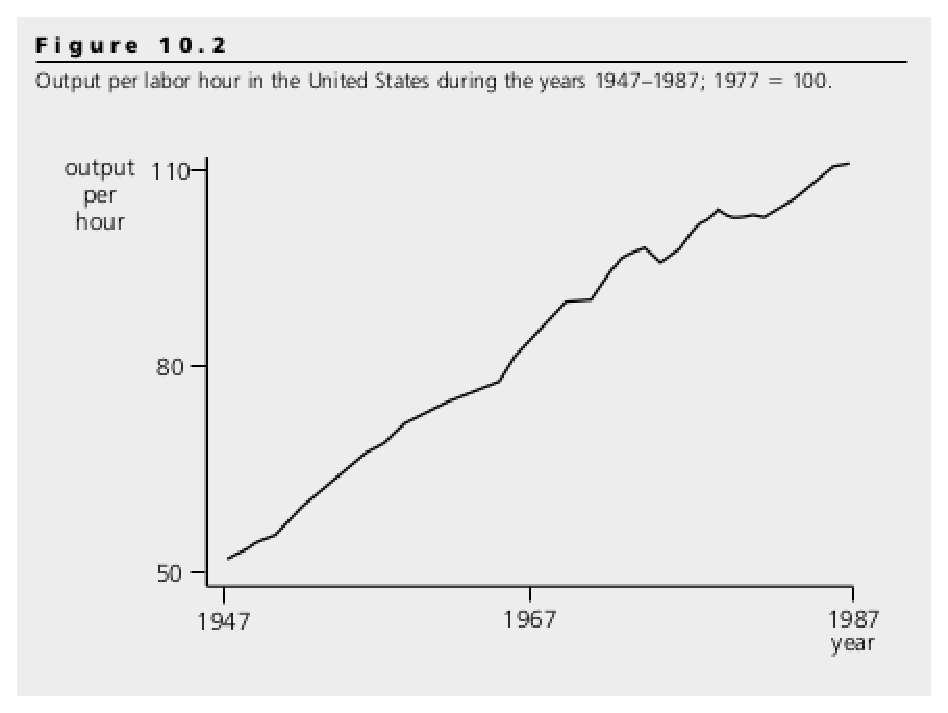
\includegraphics[scale = 0.5]{pictures/figure_10_2.eps}
\caption{Časová řada s lineárním trendem}
\label{figure_10_2}
\end{figure}

Mnoho časových řad je charakteristických exponenciálním trendem, 
což znamená konstantní relativní změnu v čase. V praxi 
exponenciální trend často podchycujeme pomocí modelu
\begin{equation}
\log(y_t) = \beta_0 + \beta_1 t + e_t, ~~~ t = 1, 2, ...,
\end{equation}
kde $\beta_1$ označujeme jako míru růstu $y$.

\begin{figure}[htp]
\centering
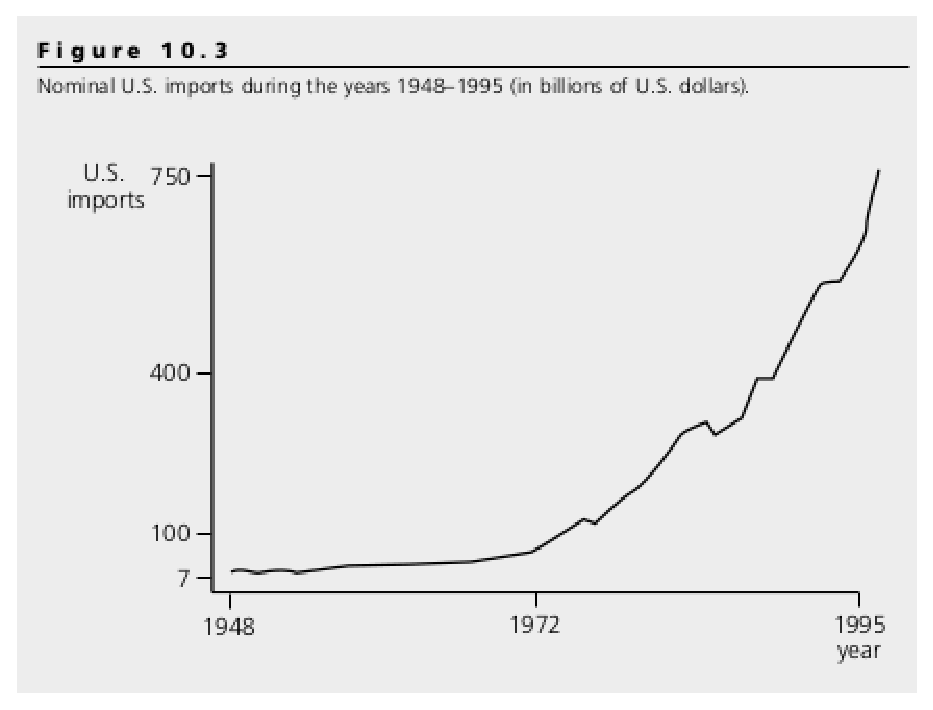
\includegraphics[scale = 0.5]{pictures/figure_10_3.eps}
\caption{Časová řada s exponenciálním trendem}
\label{figure_10_3}
\end{figure}

Ačkoliv lineární a exponenciální trendy jsou nejběžnější, 
můžeme se občas setkat také komplikovanějšími časovými trendy. Jako příklad uveďme 
model s kvadratickým trendem
\begin{equation}
y_t = \alpha_0 + \alpha_1 t + \alpha_2 t^2 + e_t,
\end{equation}
který je vhodný např. pro časové řady, ve kterých je rostoucí 
trend následovaný klesajícím trendem.

\subsubsection{Časové trendy a zdánlivá korelace}

Trendové proměnné neporušují žádný z předpokladů TS.1 až 
TS.6. Nicméně je důležité si uvědomit, že skryté faktory, 
které způsobují trend v $y$, mohou být také korelovány s 
nezávislými veličinami. Pokud bychom toto nebrali v potaz, 
vystavovali bychom se riziku tzv. zavádějící korelace (spurious 
correlation), kdy zdánlivá souvislost mezi dvěma náhodnými 
veličinami je dána pouze tím, je obě sledují obdobný trend. 
Přidáním časového trendu do modelu lze tento problém snadno eliminovat.

Pro ilustraci uvažujme nezávislé veličiny $x_{t1}$ a $x_{t2}$, 
které sledují lineární trend, a model
\begin{equation}
y_t = \beta_0 + \beta_1 x_{t1} + \beta_2 x_{t2} + \beta_3 t + u_t.
\end{equation}
Tento model zapadá do obecné metodologie vícerozměrného 
regresního modelu, protože $t$ můžeme chápat jako další 
nezávislou veličinu, tj. $t = x_{t3}$. Díky zohlednění 
časového trendu v modelu může $y_t$ lineárně růst popř. klesat 
v čase. Jestliže výše uvedený model splňuje předpoklady TS.1 až 
TS.3, pak vynechání $t$ z regresního modelu má za následek 
zkreslené odhady parametrů $\beta_1$ a $\beta_2$ v důsledku 
vynechání relevantní vysvětlující proměnné.

\subsubsection{Interpretace sklonu regresního modelu a odstranění trendu}

Jestliže (stejně jako ve výše uvedeném příkladě) provádíme regresi 
$y_i$ na $x_{t1}$, $x_{t2}$ a $t$, získáme odhad modelu ve tvaru
\begin{equation}
\hat{y}_t = \hat{\beta}_0 + \hat{\beta}_1 x_{t1} + \hat{\beta}_{t2} + 
\hat{\beta}_3 t.
\end{equation}

Odhady $\hat{\beta}_1$ a $\hat{\beta}_2$ však lze získat také 
následujícím způsobem. Nejprve provedeme regresi $y_t$, $x_{t1}$ a $x_{t2}$ na konstantu a 
časový trend $t$, čímž získáme rezidua $\ddot{y}_t$, 
$\ddot{x}_{t1}$ a $\ddot{x}_{t2}$ pro $t = 1, 2, ..., n$, např.
\begin{equation}
\ddot{y}_t = y_t - \hat{\alpha}_0 + \hat{\alpha}_1 t.
\end{equation}
O $\ddot{y}_t$ můžeme uvažovat jako o veličině, ze které jsme 
odstranili lineární trend. Pro odstranění trendu jsme museli nejprve
odhadnout model
\begin{equation}
y_t = \alpha_0 + \alpha_1 t + e_t
\end{equation}
pomocí OLS; rezidua z této regrese, tj. $\hat{e}_t = \ddot{y}_t$, 
jsou zbavené případného lineárního trendu. Podobná interpretace 
platí také pro $\ddot{x}_{t1}$ a $\ddot{x}_{t2}$.

Následně provedeme regresi $\ddot{y}_t$ na $\ddot{x}_{t1}$ a 
$\ddot{x}_{t2}$.\footnote{Do regresního modelu není třeba není 
třeba zahrnout průsečík. Pokud ho zahrneme, bude odhadnut na nulu.} 
Odhady sklonů tohoto regresního modelu budou odpovídat odhadům 
sklonů regresního modelu (10.31). To znamená, že odhady sklonu z 
(10.31) můžeme interpretovat jako odhady po odstranění lineárního 
trendu. Analogicky můžeme postupovat také v případě vícero 
vysvětlujících veličin či v případě exponenciálního či 
kvadratického trendu.

Pokud bychom z modelu (10.31) odstranili $t$ jako nezávislou 
veličinu, k odstranění trendu by nedošlo. Pak by se mohlo zdát, 
že na vývoj $y_t$ má vliv jedno či vícero $x_{tj}$. To by však 
mohlo být způsobeno pouze tím, že všechny tyto veličiny zahrnují 
časový trend.

Interpretace $\hat{\beta}_1$ a $\hat{\beta}_2$ ukazuje, že je vhodné 
zahrnout časový trend do regresního modelu, jestliže některá z 
nezávislých veličin sleduje trend, i když $y_t$ v sobě trend 
neobsahuje. V opačném případě by se totiž mohlo stát, že by 
vysvětlující veličina nevykazovala vazbu na $y_t$, ačkoliv by 
její pohyb okolo trendu na vývoj $y_t$ vliv měl.

\subsubsection{Výpočet $R^2$ v případě, že závislá veličina 
sleduje trend}

Při porovnání s modely založenými na průřezových datech je $R^2$ regresních modelů časových řad často velmi 
vysoké.
To může být způsobeno tím, že závislá veličina sleduje 
časový trend. Připomeňme, že
\begin{equation}
\bar{R}^2 = 1 - \frac{\hat{\sigma}^2_u}{\hat{\sigma}^2_y},
\end{equation}
kde $\hat{\sigma}^2_u$ je nestranná funkce odhadu rozptylu chyby 
regresního modelu a $\hat{\sigma}^2_y = \frac{SST}{n - 1} = 
\frac{\sum_{t = 1}^n(y_t - \bar{y})^2}{n - 1}$. Jestliže $E[y_t]$ 
sleduje např. lineární trend, pak $\frac{SST}{n - 1}$ není 
nestranná a konzistentní funkce odhadu $var[y_t]$. Ve skutečnosti 
může $\frac{SST}{n - 1}$ výrazným způsobem nadhodnocovat rozptyl 
$y_t$, protože nezohledňuje trend obsažený v $y_t$.

Nejjednodušším řešením je vypočíst $R^2$ po té, co byl ze 
závislé veličiny odstraněn trend, tj. jako
\begin{equation}
R^2 = 1 - \frac{\hat{\sigma}^2_u}{\sum_{t = 1}^n \ddot{y}_t^2}.
\end{equation}
Protože $\sum_{t = 1}^n \ddot{y}_t^2 \le \sum_{t = 1}^n (y_t - 
\bar{y})^2$, platí $R^2 \le \bar{R}^2$. Pokud $y_t$ obsahuje silný 
trend, může být $R^2$ výrazně nižší než $\bar{R}^2$. $R^2$ tak
lépe vysvětluje, jak je $y_t$ ovlivněno $x_{t1}$ a $x_{t2}$, 
protože zohledňuje případnou existenci časového trendu.

Korigované $R^2$ lze vypočíst analogicky dle (10.35) s tím, že 
$\hat{\sigma}^2_u$ vydělíme $n - 4$, protože to je počet stupňů 
volnosti v (10.31), a $\sum_{t = 1}^n \ddot{y}_t^2$ vydělíme $n - 2$, 
protože při odstranění trendu z $y_1$ pomocí (10.33) odhadujeme dva parametry.

Závěrem bychom měli zdůraznit, že při výpočtu $R^2$ formy $F$ statistiky pro účely testování vícero 
lineárních omezení používáme klasické $R^2$ bez odstranění 
trendu. Důvodem je, že $R^2$ forma $F$ statistiky je pouze 
výpočetní nástroj, a proto je žádoucí použít klasickou formu $R^2$.

\subsubsection{Sezónnost}

Mnoho časových řady vykazuje známky tzv. sezónností. Sezónnost chápeme 
jako situaci, kdy je časová řada výrazným způsobem 
ovlivněna aktuálním měsícem popř. ročním obdobím. Za časové 
řady, které vykazují znaky sezónnosti, můžeme považovat např. 
výnosy v zemědělství nebo počet udělených stavebních povolení. 
Některé řady mohou obsahovat jak časový trend, tak sezónnost - 
typickým příkladem takovéto řady je např. vývoj HDP.

Z časových řad, které jsou publikované statistickými úřady, je 
sezónnost velice často odstraněna. Existuje mnoho způsobů, jak z 
časové řady sezónnost odstranit, nicméně detailní popis odpovídajících 
postupů překračuje záběr této knihy. Proto si vysvětlíme pouze 
jednu relativně přímočarou metodu.

Nejjednodušším způsobem, jak odstranit sezónnost z časové řady, je pomocí 
binárních veličin. Předpokládejme, že máme k dispozici 
měsíční data, a uvažujme následující regresní model
\begin{multline}
y_t = \beta_0 + \delta_1 feb_t + \delta_2 mar_t + \delta_3 apr_t + 
...\\ 
+ \delta_{11} dec_t + \beta_1 x_{t1} + ... + \beta_k x_{tk} + u_t,
\end{multline}
kde $feb_t$, $mar_t$, ..., $dec_t$ představují binární veličiny, 
které indikují kalendářní měsíc dané časové periody 
$t$.\footnote{Měsíc leden byl záměrně vynechán, abychom se 
vyhnuli tzv. pasti binární veličiny.} 
Pokud $y_t$ nevykazuje sezónnost, pak jsou $\delta_1$ až $\delta_{11}$ 
sdruženě statisticky nevýznamné, což lze otestovat pomocí $F$ 
statistiky. Analogicky lze postupovat, pokud máme k dispozici 
čtvrtletní namísto měsíčních dat.

Sezónnost lze z časových řad odstranit podobným způsobem, jakým 
jsme odstranily trend. Uvažujme rovnici (10.36) s $k = 2$. Odhady 
$\hat{\beta}_1$ a $\hat{\beta}_2$ lze získat následovně.

Nejprve provedeme regresi $y_t$, $x_{t1}$ a $x_{t2}$ na konstantu a 
binární veličiny reprezentující měsíce únor až prosinec, 
abychom získali rezidua $\ddot{y}_t$, $\ddot{x}_{t1}$ a 
$\ddot{x}_{t2}$ pro všechna $t = 1, 2, ..., n$. Jako příklad uveďme
\begin{equation}
\ddot{y}_t = y_t - \hat{\alpha}_0 - \hat{\alpha}_1 feb_t - 
\hat{\alpha}_2 mar_t - ... - \hat{\alpha}_{11} dec_t,
\end{equation}
čímž jsme odstranili sezónnost z měsíční časové řady $y_t$. 
Podobnou interpretaci lze použít také v případě časových řad 
$\ddot{x}_{t1}$ a $\ddot{x}_{t2}$. Následně provedeme regresi $\ddot{y}_t$ na $\ddot{x}_{t1}$ a 
$\ddot{x}_{t2}$, čímž získáme odhady $\hat{\beta}_1$ a $\hat{\beta}_2$.

V případě, že $y_t$ vykazuje silné známky sezónnosti, je vhodné tuto skutečnost zohlednit v $R^2$ podobně, jak tomu bylo v případě časového trendu. Tímto způsobem se zbavíme sezónních vlivů, které nejsou vysvětleny pomocí $x_{tj}$.

Jak jsme již dříve zmínili, mnoho časových řad vykazuje známky 
jak časového trendu, tak sezónnosti. V takovémto případě by 
regresní model měl zahrnovat časový trend i sezónní 
binární veličiny.

\chapter{Aplikace OLS na časové řady}

\section{Stacionární a slabě závislá časová řada}

\subsection{Stacionární a nestacionární časová řada}

\subsubsection{Stacionární stochastický proces}

Stochastický 
proces ${x_t: t = 1, 2, ...}$ je stacionární, jestliže pro 
libovolný výběr časových indexů $1 \le t_1 < t_2 < ... < t_m$ je 
sdružené rozdělení $(x_{t_1}, x_{t_2}, ..., x_{t_m})$ stejné jako 
sdružené rozdělení $(x_{t_1 + h}, x_{t_2 + h}, ..., x_{t_m + h})$ 
pro všechna celá čísla $h \ge 1$.

Zjednodušeně může říci, že 
stacionární časová řada je časová řada, jejíž 
pravděpodobnostní rozdělení je stabilní v čase. 
Pravděpodobnostní rozdělení $x_1$ je tak stejné jako $x_2$ nebo 
$x_3$ - posloupnost $\{x_t; t = 1, 2, ...\}$ sleduje identické 
pravděpodobnostní rozdělení.

Samotná stacionarita však vyžaduje více - např. sdružené 
rozdělení $(x_1, x_2)$ musí být identické se sdruženým 
pravděpodobnostním rozdělením $(x_t, x_{t + 1})$ pro libovolné $t 
\ge 1$. To znamená, že korelace mezi dvěma po sobě jdoucími členy 
časové řady je konstantní napříč celou časovou řadou.

Stochastický proces, který není stacionární, nazýváme 
nestacionárním stochastickým procesem. Příkladem takovéhoto 
procesu je časová řada s trendem, se kterou jsme se setkali v 
minulé kapitole.

\subsubsection{Kovariančně stacionární proces}

Stochastický proces $\{x_t: t = 1, 2, ...\}$ s konečným druhým 
momentem $[E[x_i^2] < \infty]$ je kovariančně stacionární, pokud 
(1) $E[x_t]$ je konstantní, (2) $var[x_t]$ je konstantní a (3) pro 
libovolné $t$ a $h \ge 1$ je $cov[x_t, x_{t + h}]$ pouze funkcí $h$ a 
nikoliv funkcí $t$.

Kovarianční stacionarita se zaměřuje pouze na první dva momenty 
stochastického procesu, kde střední hodnota a rozptyl jsou 
konstantní v čase a kovariance mezi $x_t$ a $x_{t + h}$ závisí 
pouze na jejich vzájemné vzdálenosti $h$.

Jestliže má stacionární proces konečný druhý moment, pak musí 
být kovariančně stacionární. Opačné tvrzení však nemusí být pravdivé.

\subsubsection{Význam stacionarity}

Pokud chceme analyzovat vazby mezi dvěma proměnnými pomocí 
regresní analýzy, musí předpokládat jistou formu jejich stability v 
čase. Jestliže by se vazba mezi těmito dvěma proměnnými (např. mezi $x$ a 
$y$) náhodně měnila s každou časovou periodou, nemohli bychom 
doufat, že této vazbě porozumíme, pokud bychom měli k dispozici 
pouze jednu realizaci podkladového procesu.

\subsection{Slabě závislá časová řada}

Kovariančně stacionární časová 
řada je slabě závislá, pokud korelace mezi $x_t$ a $x_{t + h}$ 
konverguje dostatečně rychle k nule s tím, jak $h \rightarrow \infty$.
Kovariančně stacionární řady, kde $corr[x_t, x_{t+h}] \rightarrow 
0$ pro $h \rightarrow \infty$, nazýváme asymptoticky nekorelované.

Předpoklad slabé závislosti je pro regresní analýzu důležitý, 
protože nahrazuje předpoklad náhodného výběru, který implikuje 
platnost zákona velkých čísel a centrální limitní věty. 
Stacionární slabě závislá časová řada je tak ideální pro 
účely vícerozměrné regresní analýzy.

\subsubsection{Proces klouzavého průměru řádu jedna}

Uvažujme příklad slabě závislé řady
\begin{equation}
x_t = e_t + \alpha_1 e_{t - 1}, ~~~ t = 1, 2, ...,
\end{equation}
kde $\{e_t, t = 0, 1, ...\}$ je nezávislá stejnoměrně rozdělená 
posloupnost s nulovou střední hodnotou a rozptylem $\sigma^2_e$. 
Proces $\{x_t\}$ nazýváme procesem klouzavého průměru řádu jedna 
[moving average process of order one; MA(1)].

Proč je MA(1) proces slabě závislý? Je zřejmé, že po sobě 
jdoucí členy $x_t$ a $x_{t + 1}$ jsou 
korelované. Protože $x_{t + 1} = e_{t + 1} + \alpha_1 e_t$, je 
$cov[x_t, x_{t + 1}]$ rovno $\alpha_1 var[e_t] = \alpha_t \sigma^2_e$. 
A protože $var[x_t] = (1 + \alpha_1^2)\sigma^2_e$, je $corr[x_t, x_{t + 
1}]$ rovno $\frac{\alpha_1}{1 + \alpha_1^2}$. Jakmile se však 
zaměříme na členy posloupnosti, které jsou od sebe dvě a více 
časových period, zjistíme, že jsou nekorelované, protože jsou 
nezávislé. Z důvodu předpokladu nezávislého stejnoměrného 
rozdělení $e_t$ je $\{x_t\}$ stacionární. MA(1) je tak
stacionární slabě závislá posloupností, a proto na ni lze aplikovat 
zákon velkých čísel a centrální limitní větu.

\subsubsection{Autoregresivní proces řádu jedna}

Dalším populárním příkladem stacionární slabě závislé řady 
je tzv. autoregresivní proces řádu jedna [autoregressive process of 
order one; AR(1)].
\begin{equation}
y_t = \rho_1 y_{t - 1} + e_t, ~~~ t = 1, 2, ...
\end{equation}
Počáteční bod řady je $y_0$ a $\{e_t: t = 1, 2, ... \}$ je 
nezávislá stejnoměrně rozdělená posloupnost s nulovou střední 
hodnotou a rozptylem $\sigma^2_e$. Dále předpokládáme, že $e_t$ je 
nezávislé na $y_0$ a že $E[y_0] = 0$.

Klíčovým předpokladem pro slabou závislost AR(1) procesu je tzv. 
podmínka stability $|\rho_1| < 1$. Pak nazýváme $\{y_t\}$ stabilním 
AR(1) procesem.

Předpokládejme, že je výše uvedený proces kovariančně 
stabilní.\footnote{Lze dokázat, že $\{y_t\}$ je striktně 
stacionární. Tento důkaz však přesahuje záběr naší knihy.} 
Tento předpoklad implikuje $E[y_t] = E[y_{t - 1}]$, což pro (11.2) s 
$\rho_1 \ne 1$ může nastat pouze pro $E[y_t] = 0$. Vzhledem k tomu, 
že $e_t$ a $y_{t - 1}$ jsou nezávislé, platí $var[y_t] = \rho_1^2 
\sigma^2_y + \sigma_e^2$. Protože dle podmínky stability platí 
$\rho_1^2 < 1$, získáváme
\begin{equation}
\sigma^2_y = \frac{\sigma_e^2}{1 - \rho_1^2}
\end{equation}

Kovarianci mezi $y_t$ a $y_{t + h}$ pro $h \ge 1$ lze pak odvodit 
následujícím způsobem.
\begin{multline}
y_{t + h} = \rho_1 y_{y + h - 1} + e_{t + h} = \rho_1(\rho_1 y_{t + h - 
2} + e_{t + h -1}) + e_{t + h}\\
= \rho_1^2 y_{t + h - 2} + \rho+1 e_{t + h - 1} + e_{t + h} = ...\\
= \rho_1^h y_t + \rho_1^{h - 1} e_{t + 1} + ... + \rho_1 e_{t + h - 1} 
+ e_{t + h}
\end{multline}
Protože $E[y_t] = 0$, můžeme poslední rovnici vynásobit $y_t$ a 
aplikovat očekávanou hodnotu, abychom získali $cov[y_t, y_{t + h}]$. 
S využitím skutečnosti, že $e_{t + j}$ je nekorelované s $y_t$, 
získáváme
\begin{multline}
  cov[y_t, y_{t + h}]\\
  = E[y_t, y_{t + h}] = \rho_1^h E[y_t^2] + \rho_1^{h 
- 1} E[y_t e_{t + 1}] + ... + E[y_t e_{t + h}]\\
= \rho_1^h E[y_t^2] = \rho^h \sigma_y^2.
\end{multline}
Protože $\sigma_y$ je standardní směrodatná odchylka jak pro $y_t$ 
tak pro $y_{t + h}$, můžeme korelaci mezi $y_t$ a $y_{t + h}$ 
definovat jako
\begin{equation}
corr[y_t, y_{t + h}] = \frac{cov(y_t, y_{t + h})}{\sigma_y \sigma_y} = 
\rho_1^h.
\end{equation}
Korelace dvou po sobě jdoucích členů časové řady je $\rho_1$. Je 
zřejmé, že i když je tato korelace vysoká - řekněme 0.90 - 
korelace mezi $y_t$ a $y_{t + h}$ klesá velmi rychle k nule s tím, 
jak $h \rightarrow \infty$. Proto můžeme AR(1) považovat za slabě 
závislý proces.

Na závěr zdůrazněme, že časová řada sledující trend, 
ačkoliv nestacionární, může být slabě závislá. Časovou řadu, 
která je po odstranění trendu jak stacionární tak slabě 
závislá, nazýváme trendově stacionárním procesem.

\section{Asymptotické vlastnosti OLS}

\begin{assumption}[TS.1' - linearita a slabá závislost]
Uvažujme stejný model jako v případě předpokladu TS.1. Nyní však přidejme předpoklad, že $\{(x_t, y_t): t = 1, 2, ...\}$ je stacionární a slabě závislý proces. V tomto případě lze na výběrové průměry aplikovat zákon velkých čísel a centrální limitní větu.

\raggedleft{$\clubsuit$}
\end{assumption}

Důležitým rozdílem mezi TS.1 a TS.1' je předpoklad slabé závislosti.

\begin{assumption}[TS.2' - neexistence perfektní kolinearity]
Stejný předpoklad jako TS.2.

\raggedleft{$\clubsuit$}
\end{assumption}

\begin{assumption}[TS.3' - nulová podmíněná střední hodnota]
Vysvětlující veličiny $x_t = (x_{t1}, x_{t2}, ..., x_{tj})$ jsou souběžně exogenní tak, jak je tomu v rovnici (10.16), tj. $E[u_t|x_t] = 0$.
  
\raggedleft{$\clubsuit$}
\end{assumption}

TS.3' je mnohem méně restriktivní než TS.3, protože TS.3' neklade žádná omezení na to, jaký má být vztah mezi $u_t$ a vysvětlujícími veličinami v ostatních časových periodách. Nicméně stacionarita implikuje, že pokud souběžná exogenita platí pro jednu časovou periodu, pak platí pro všechny časové periody. Pokud bychom se zbavili předpokladu stacionarity, museli bychom požadovat splnění TS.3' pro všechny časové periody $t = 1, 2, ...$.

Předpoklad konzistentnosti OLS, který je představen ve větě 11.1, pouze vyžaduje, aby $u_t$ mělo nulovou nepodmíněnou střední hodnotu a bylo nekorelované s libovolným $x_{ij}$, tj.
\begin{equation}
E[u_t] = 0, ~~~ cov[x_{tj}, u_t] = 0, ~~~ j = 1, 2, ..., k.
\end{equation}

V následujícím textu budeme převážně pracovat s předpokladem nulové podmíněné střední hodnoty, protože vede k nejpřímější definici asymptotické analýzy.

\begin{theorem}[Konzistentnost OLS]
Při splnění předpokladů TS.1', TS.2' a TS.3' jsou OLS odhady konzistentní, tj. $plim \hat{\beta}_j = \beta_j$ pro $j = 0, 1, ..., k$.
  
\raggedleft{$\clubsuit$}
\end{theorem}

Mezi větami 10.1 a 11.1 existuje několik praktických odlišností. Za prvé, ve větě 11.1 jsme došli k závěru, že OLS odhady jsou konzistentní. Tato věta nám však neříká nic o jejich nestrannosti. Za druhé, ve větě 11.1 jsme na jedné straně oslabili význam, ve kterém musí být vysvětlující veličiny exogenní, na druhé straně avšak musí být podkladová časová řada slabě závislá. Slabá závislost je klíčová pro získání distribucí odhadů regresních parametrů; tomuto tématu se budeme věnovat v následující kapitole.

Pro ilustraci uvažujme AR(1) proces
\begin{equation}
y_t = \beta_0 + \beta_1 y_{t - 1} + u_t,
\end{equation}
kde
\begin{equation}
E[u_t | y_{t - 1}, y_{t - 2}, ...] = 0.
\end{equation}
Pokud spojíme tyto dvě rovnice, získáme
\begin{equation}
E[y_t | y_{t - 1}, y_{t - 2}, ...] = E[y_t | y_{t - 1}] = \beta_0 + \beta_1 y_{t - 1}.
\end{equation}

Protože v roli vysvětlující veličiny vystupuje pouze $y_{t-1}$, implikuje (11.9) platnost předpokladu TS.3'. Předpoklad striktní exogenity, tj. předpoklad TS.3, který je nezbytný pro nezkreslenost OLS odhadů, splněn není. V AR(1) procesu vysvětlující veličiny obsahují všechny hodnoty $y$ s výjimkou té poslední, tj. $(y_0, y_1, ..., y_{n - 1})$. Předpoklad TS.3 však vyžaduje, aby pro všechna $t$ bylo $u_t$ nekorelováno s $y_0, y_1, ..., y_{n - 1}$, což zcela zřejmě není splněno. Navíc, protože $E[u_t] = 0$ a $corr[y_{t - 1}, u_t] = 0$, musí být $u_t$ a $y_t$ korelováno.
\begin{multline}
cov[y_t, u_t] = E[y_t, u_t] - E[y_t]E[u_t] = E[y_t, u_t]\\
= E[(\beta_0 + \beta_1 y_{t - 1} + u_t)u_t] = \beta_0 E[u_t] + \beta_1 E[y_{t - 1} u_t] + E[u^2_t]\\
= E[u^2_t] = E[u^2_t] - E[u_t]^2 = var[u_t] > 0  
\end{multline}
Je tedy zřejmé, že AR(1) nemůže splňovat předpoklad TS.3.

Pro splnění předpokladu slabé závislosti musí být $|\beta_1| < 1$. Jestliže je tento předpoklad splněn, pak věta 11.1 implikuje, že OLS odhady jsou konzistentní. Bohužel $\hat{\beta}_1$ není nestranný a míra zkreslení může být značná, pokud se jedná o vzorek malého rozsahu nebo pokud je $\beta_1$ blízké jedné.\footnote{Pro $\beta_1$ blízké jedné může $\hat{\beta}_1$ výrazně podhodnocovat skutečnou hodnotu $\beta_1$.} Pro vzorky středního nebo velkého rozsahu by $\hat{\beta}_1$ mělo být dobrým odhadem $\beta_1$.

\begin{assumption}[TS.4' - homoskedasticita]
Chyby regresního modelu jsou souběžně homoskedasticitní, tj. $var[u_t | x_t] = \sigma^2$.

\raggedleft{$\clubsuit$}
\end{assumption}

\begin{assumption}[TS.5' - neexistence autokorelace]
Pro všechna $t \ne s$ platí $E[u_tu_s|x_t, x_s] = 0$.

\raggedleft{$\clubsuit$}
\end{assumption}

Všimněme si, že v TS.4' na rozdíl od TS.4 podmiňujeme pouze na vysvětlující veličiny v čase $t$. V TS.5' pak podmiňujeme pouze na vysvětlující veličiny v časových periodách, které se shodují s $u_t$ a $u_s$. V praxi však velice často ignorujeme podmínění na $x_t$ a $x_s$ a namísto toho uvažujeme, že $u_t$ a $u_s$ jsou nepodmíněně nekorelované pro všechna $t \ne s$.

Autokorelace je častý problém statických modelů a modelů s konečným rozdělením zpoždění - neexistuje nic, co by garantovalo neexistenci korelace $u_t$ v čase. Nicméně TS.5' platí pro AR(1) proces tak, jak je formulován v (11.8) a (11.9). Protože vysvětlující veličina v čase $t$ je $y_{t - 1}$, musíme dokázat, že $E[u_t u_s | y_{t - 1} y_{s - 1}] = 0$ pro všechna $t \ne s$. Pro ilustraci uvažujme $s < t$.\footnote{Na opačný případ lze aplikovat princip symetrie.} Protože $u_s = y_s - \beta_0 - \beta_1 y_{s - 1}$, je $u_s$ funkcí $y$ před časem $t$. Dle (11.9) platí $E[u_t|u_s, y_{t - 1}, y_{s - 1}] = 0$, a proto $E[u_t u_s| u_s, y_{t - 1}, y_{s - 1}] = u_s E[u_t | y_{t - 1}, y_{s - 1}] = 0$. Zákon iterované střední hodnoty (law of iterated expectations) implikuje $E[u_t s_t | y_{t - 1}, y_{s - 1}] = 0$. Toto je velmi důležitý závěr - pokud (11.8) obsahuje pouze jedno zpoždění, nejsou chyby regresního modelu autokorelované.

\begin{theorem}[Asymptotická normalita OLS odhadů]
Při splnění předpokladů TS.1' až TS.5' sledují OLS odhady asymptoticky normální rozdělení. Také klasické $t$ a $F$ statistiky jsou asymptoticky platné.
  
\raggedleft{$\clubsuit$}
\end{theorem}

Výše uvedená věta tedy říká, že i když nejsou předpoklady klasického lineárního modelu bez zbytku splněny, jsou OLS odhady konzistentní a lze použít obvyklé procedury pro jejich odhad a to včetně stanovení intervalů spolehlivosti.

Při splnění předpokladů TS.1' až TS.5' lze dokázat, že OLS odhady jsou asymptoticky efektivní v rámci rodiny odhadů popsaných ve větě 5.3.\footnote{Pouze nahradíme index náhodného výběru $i$ časovým indexem $t$.} Také modely, které zahrnují trend, mohou splňovat požadavky TS.1' až TS.5' za předpokladu, že jsou trendově stacionární. Pokud je časový trend explicitně zahrnut do regresního modelu, lze také použít obvyklé postupy pro odhad parametrů.

\section{Persistentní časové řady v regresní analýze}

V praxi se poměrně často setkáváme s časovými řadami, které nesplňují podmínku slabé závislosti. Aplikace regresní analýzy na časové řady, které vykazují silnou závislost v čase, nepředstavuje zásadní problém, pokud jsou splněny CLM předpoklady, které jsme představili v kapitole 10. Nicméně stanovení intervalů spolehlivosti jednotlivých odhadů může být značně zavádějící, protože se již nelze spolehnout na zákon velých čísel a centrální limitní větu.

\subsection{Persistentní časové řady}

AR(1) proces je slabě závislý, pokud $|\rho_1| < 1$. Nicméně v praxi mnoho časových řad lépe charakterizuje model
\begin{equation}
y_t = y_{t - 1} + e_t, ~~~ t = 1, 2, ...,
\end{equation}
kde $\{e_t: t = 1, 2, ...\}$ sleduje nezávislé identické pravděpodobnostní rozdělení s nulovou střední hodnotou a rozptylem $\sigma^2$. Tento proces nazýváme náhodnou procházkou. Předpokládejme, že $y_0$ je nezávislé na $e_t$ pro všechna $t \ge 1$. Pak lze střední hodnotu $t_t$ snadno určit pomocí opakované substituce
\begin{equation}
y_t = e_t + e_{t - 1} + ... + e_1 + y_0
\end{equation}
a následnou aplikací očekávané hodnoty
\begin{equation}
E[y_t] = E[e_t] + E[e_{t - 1}] + ... + E[e_1] + E[y_0] = E[y_0].
\end{equation}
Očekávaná hodnota náhodné procházky je tak nezávislá na čase $t$. Obvyklý předpoklad je $y_0 = 0$, což implikuje $E[y_t] = 0$ pro všechna $t$.

Naproti tomu rozptyl náhodné procházky narůstá s časem $t$, a proto se nejedná o stacionární proces. Předpokládejme, že $y_0$ je nenáhodné, tj. $var[y_0] = 0$. Protože $\{e_t\}$ sleduje identické nezávislé rozdělení, platí
\begin{equation}
var[y_t] = var[e_t] + var[e_{t - 1}] + ... + var[e_t] = \sigma_e^2 t.
\end{equation}
Navíc náhodná procházka vykazuje značně persistentní chování, což znamená, že hodnota $y$ dnes je důležitá pro určení hodnoty $y$ i ve velmi vzdálené budoucnosti. Pro ilustraci rozepišme $h$ časových period jako
\begin{equation}
y_{t + h} = e_{t + h} + e_{t + h - 1} + ... + e_{t + 1} + y_t.
\end{equation}
Předpokládejme, že chceme vypočíst očekávanou hodnotu $y_{t + h}$ pro danou hodnotu $y_t$. Z výše uvedené rovnice je zřejmé, že
\begin{equation}
E[y_{t + h}|y_t] = y_t.
\end{equation}
Jinými slovy, nejlepším odhadem budoucí hodnoty $y_{t + h}$ je současná hodnota $y_t$ a to bez ohledu na to, jak vzdálenou budoucnost uvažujeme. To lze postavit do kontrastu se stabilním AR(1) procesem, kde byl podobný postup použit jako důkaz pro
\begin{equation}
E[y_{t + h} | y_t] = \rho_1^h y_t,
\end{equation}
kde $E[y_{t + h}|y_t]$ se blíží nepodmíněné střední hodnotě $E[y_t] = 0$ s tím, jak $h \rightarrow \infty$, a to bez ohledu na hodnotu $y_t$.

Lze dokázat, že v případě náhodné procházky $\{y_t\}$ se korelace mezi $y_t$ a $y_{t + h}$ pro dostatečně velké $t$ blíží jedné. Za předpokladu $var[y_0] = 0$ totiž platí
\begin{equation}
corr[y_t, y_{t + h}] = \sqrt{\frac{t}{t + h}}.
\end{equation}
Korelace tak závisí na počátečním bodu $t$, a proto $\{y_t\}$ není kovariančně stacionární. Ačkoliv pro fixní $t$ se korelace blíží nule s tím, jak se $h$ blíží nekonečnu, není tato konvergence dostatečně ``rychlá''.  Pro libovolné $h$ lze vždy zvolit $t$ dostatečně vysoké na to, aby se $corr[y_t, y_{t + h}]$ blížilo jedné. Náhodná procházka tak nesplňuje požadavek na asymptoticky nekorelovanou řadu.

Jak nározně ilustruje následující graf, je v praxi velmi obtížné vizuálně rozlišit, zda-li je daný proces náhodnou procházkou či nikoliv.
\begin{figure}[htp]
\centering
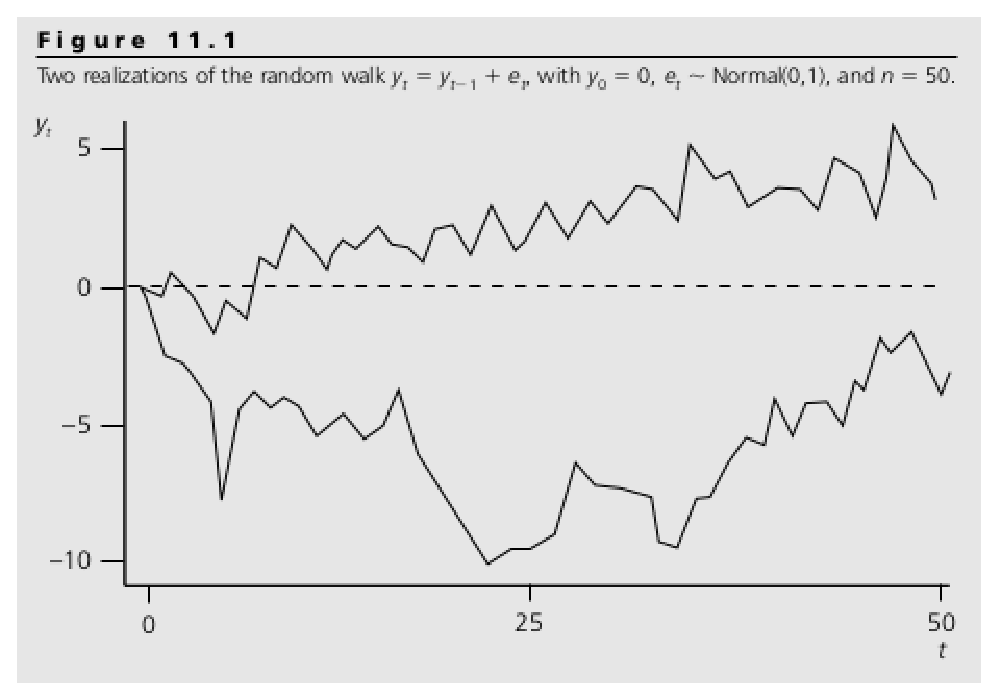
\includegraphics[scale = 0.5]{pictures/figure_11_1.eps}
\caption{Dvě náhodné procházky}
\label{figure_11_1}
\end{figure}
Náhodná procházka je specifickým příkladem tzv. procesu s jednotkovým kořenem (unit root process). Jméno procesu vychází ze skutečnosti, že se jedná o AR(1) model s $\rho_1 = 1$.

Je velmi důležité nezaměňovat časový trend s persistentním charakterem časové řady. Časová řada muže sledovat trend a přitom nebýt persistentní. Existuje však také řady, které jsou persitentní a přitom nesledují žádný trend - příkladem takové řady může být (alespoň pro určitá období) vývoj nezaměstnanosti či inflace. Velice často se však můžeme setkat s řadami, které jsou persistentní a navíc sledující trend. Triviálním příkladem takovéto řady je náhodná procházka s trendem
\begin{equation}
y_t = \alpha_0  + y_{t - 1} + e_t, ~~~ t = 1, 2, ...,
\end{equation}
kde $\{e_t: t = 1, 2, ...\}$ a $y_0$ splňují stejné podmínky jako v případě klasické náhodné procházky. Nově přibyl parametr $\alpha$, který představuje časový trend. S použitím opakované substituce lze snadno dokázat, že střední hodnota tohoto procesu je funkcí času.
\begin{multline}
  E[y_t] = E[\alpha_0t + e_t + e_{t - 1} + ... + e_t + y_0] = \alpha_0 t + E[e_t]\\
  + E[e_{t - 1}] + ... + E[e_1] + E[y_0] = \alpha_0 t
\end{multline}
Podobně jako v případě klasické náhodné procházky lze také v případě náhodná procházky s trendem dokázat, že $E[y_{t + h}|y_t] = a_0 h + y_t$. Rozptyl $y_t$ je stejný jako v případě obyčejné náhodné procházky.

Následující graf zobrazuje náhodnou procházku s trendem. Je zřejmé, že proces sleduje lineární časový trend, nicméně nemá tendenci se vracet k trendové linii.
\begin{figure}[htp]
\centering
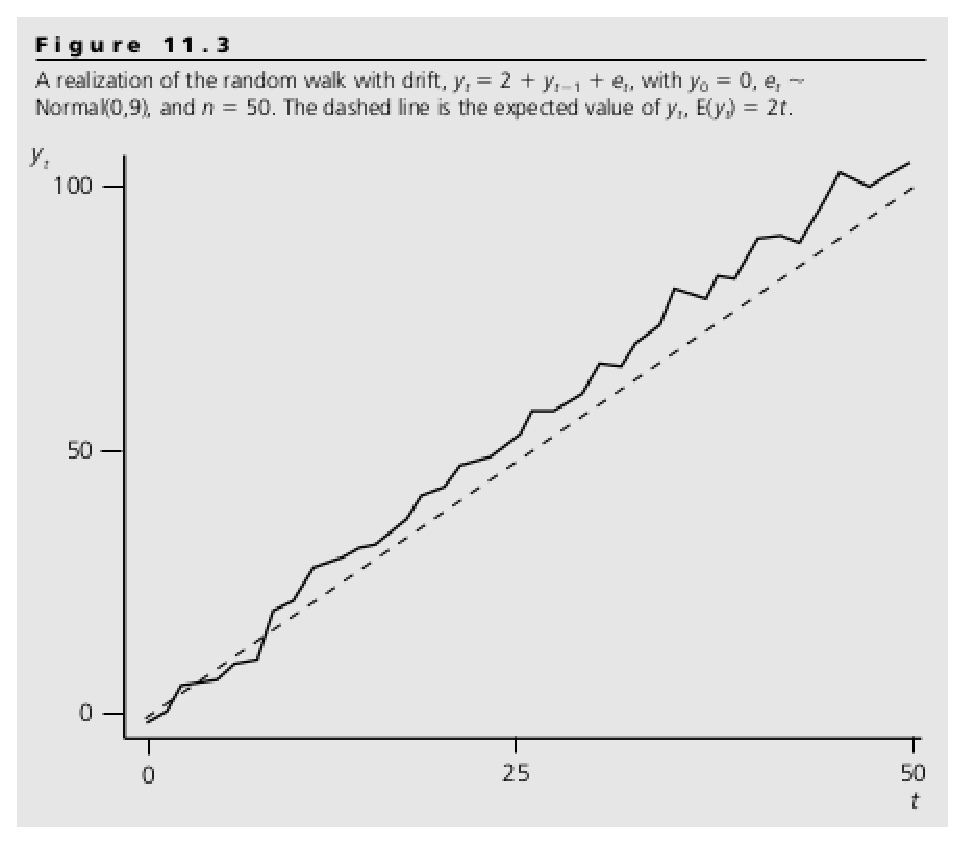
\includegraphics[scale = 0.5]{pictures/figure_11_2.eps}
\caption{Náhodná procházka s trendem}
\label{figure_11_2}
\end{figure}

Náhodná procházka s trendem je příkladem procesu s jednotkovým kořenem, protože se zjevně jedná o AR(1) s  $\rho_1 = 1$.
\begin{equation}
y_t = \alpha_0 + \rho_1 y_{t - 1} + e_t
\end{equation}

\subsubsection{Transformace persistentních časových řad}

Aplikace regresního modelu na časové řady s jednotkovým kořenem může vést k zavádějícím závěrům, pokud jsou porušeny CLM předpoklady.

O slabých závislých časových řadách říkáme, že jsou integrované stupněm nula (integrated of order zero) a značíme je jako $I(0)$. Na tyto časové řady může být aplikována regresní analýza. Procesy s jednotkovým kořenem jako je náhodná procházka (jak s trendem tak bez něj) jsou integrovány stupněm jedna a značíme je jako $I(1)$. Na takovouto časovou řadu musíme nejprve aplikovat diferenci prvního řádu, čímž získáme $I(0)$, a teprve po té ji můžeme použít jako vstup pro regresní analýzu.

Koncept $I(1)$ procesu se nejsnáze vysvětluje na náhodné procházce. Pro $y_t$ generované dle (11.12) totiž platí
\begin{equation}
\Delta y_t = y_t -  y_{t - 1} = e_t, ~~~ t = 2, 3, ...,
\end{equation}
takže $\{\Delta y_t: t = 2, 3, ...\}$ představuje identickou nezávisle rozdělenou posloupnost a je tak slabě závislé. Aplikace diference prvního řádu má však další výhodu a tou je odstranění případného lineárního časového trendu.

\subsubsection{Testování $I(1)$ procesu}

Rozhodování o tom, zda-li je realizace určité časové řady procesem s jednotkovým kořenem, je poměrně komplikované. Tématu se budeme do hloubky zabývat v kapitole 18.

Velmi jednoduchý test je založen na AR(1) modelu - proces je $I(0)$ pokud $|\rho_1| < 1$ a $I(1)$ pokud $\rho_1 = 1$. V předchozím textu jsme prokázali, že pokud je $AR(1)$ proces stabilní, pak $\rho_1 = corr[y_t, y_{t - 1}]$. Proto lze $\rho_1$ odhadnout pomocí výběrové korelace mezi $y_t$ a $y_{t - 1}$. Tuto výběrovou korelaci nazýváme autokorelací prvního řádu a značíme ji jako $\hat{\rho}_1$. S využitím zákona velkých čísel lze dokázat, že $\hat{\rho}_1$ je při splnění podmínky $|\rho_1| < 1$ konzistentním odhadem $\rho_1$.\footnote{Nicméně $\hat{\rho}_1$ není nezkresleným odhadem $\rho_1$.}

Hodnotu $\hat{\rho}_1$ pak lze použít při rozhodování o tom, zda-li je určitý proces $I(0)$ nebo $I(1)$. Teoreticky by mělo stačit určit konfidenční interval pro $\rho_1$ a zkontrolovat, zda-li obsahuje hodnotu $\rho_1 = 1$. Bohužel výběrová distribuce funkce odhadu $\hat{\rho}_1$ je extrémně odlišná populační distribuce, pokud je $\rho_1$ blízké jedné nebo výrazně menší než jedna. Prozatím tedy budeme použít $\hat{\rho}_1$ jako přibližný indikátor toho, zda-li máme na časovou řadu aplikovat diferenci prvního řádu.

Jestliže časová řada vykazuje silný trend, je vhodné aplikovat diferenci prvního řádu až po odstranění trendu. Jestliže z časové řady není odstraněn trend, pak je autoregresivní korelace výrazně nadhodnocená, což zvyšuje ``pravděpodobnost'' indikace jednotkového kořene.  

\subsection{Dynamicky kompletní modely a absence autokorelace}

Uvažujme následující jednoduchý regresní model
\begin{equation}
y_t = \beta_0 + \beta_1 z_t + u_t.
\end{equation}
Pro konzistenci OLS odhadů postačuje, pokud $E[u_t | z_t] = 0$. Obecně platí, že $\{u_t\}$ může být autokorelované. Nicméně, pokud předpokládáme
\begin{equation}
E[u_t|z_t, y_{t - 1}, z_{t - 1}, ...] = 0,
\end{equation}
pak, jak si ukážeme později, je předpoklad TS.5' splněn. Konkrétně $\{u_t\}$ není autokorelované. Rovnice (11.25) implikuje souběžnou exogenitu $z_t$, tj. $E[u_t|z_t] = 0$.

Abychom získali lepší vhled do problému, aplikujme podmíněné očekávání na (11.24) a použijme (11.25), čímž získáme
\begin{equation}
E[y_t|z_t, y_{t - 1}, z_{t - 1}, ...] = E[y_t | z_t] = \beta_0 + \beta_1 z_t + E[u_t|z_t] = \beta_0 + \beta_1 z_t.
\end{equation}
Tato rovnice nám říká, že v okamžiku fixace $z_t$ nejsou zpožděná $y$ a $z$ schopna vysvětlit aktuální hodnotu $y$. Pokud tento předpoklad není splněn, pak je $\{u_t\}$ autokorelované.

Dále uvažujme model se dvěma zpožděními.
\begin{equation}
y_t = \beta_0 + \beta_1 z_t + \beta_2 z_{t - 1} + \beta_3 z_{t - 2} + u_t
\end{equation}
Vzhledem k definici modelu má podmíněná střední hodnota tvar
\begin{equation}
E[y_t | z_t, z_{t - 1}, z_{t - 2}, z_{t - 3}, ...] = E[y_t | z_t, z_{t - 1}, z_{t - 2}].
\end{equation}
Podobně jako předchozím případě pak předpokládáme, že po fixaci $z_t$, $z_{t - 1}$ a $z_{t - 2}$ nemá žádné zpožděné $y$ a žádné $z$ se zpožděním větším než dva schopnost vysvětlit aktuální hodnotu $y$, tj.
\begin{equation}
E[y_t| z_t, y_{t - 1}, z_{t - 1}, ...] = E[y_t | z_t, z_{t - 1}, z_{t - 2}].
\end{equation}

Nakonec uvažujme obecný model
\begin{equation}
y_t = \beta_0 + \beta_1 x_{t1} + ... + \beta_k x_{tk} + u_t,
\end{equation}
kde vysvětlující veličiny $x_t = (x_{t1}, ..., x_{tk})$ mohou zahrnovat jak zpožděná $z$, tak zpožděná $y$. Rovnice (11.25) tak přejde do tvaru
\begin{equation}
E[u_t|x_t, y_{t - 1}, x_{t - 1}, ...] = 0,
\end{equation}
což vyjádřeno pomocí $y_t$ znamená
\begin{equation}
E[y_t | x_t, y_{t - 1}, x_{t - 1}, ...] = E[y_t | x_t].
\end{equation}
Jinými slovy, do matice $x_t$ byl zařazen dostatek zpožděných veličin tak, aby další zpožděné $y$ a další zpožděné vysvětlující veličiny $z$ měly ve vztahu k aktuální hodnotě $y$ nulovou vypovídající hodnotu. Takovýto model nazýváme dynamicky kompletním modelem. Protože (11.31) je ekvivalentní
\begin{equation}
E[u_t | x_t, u_{t - 1}, x_{t - 1}, u_{t - 2}, ...] = 0,
\end{equation}
lze dokázat, že dynamicky kompletní model splňuje předpoklad TS.5'. Pro ilustraci uvažujme $s < t$; s využitím zákona o iterované střední hodnotě pak získáme
\begin{multline}
  E[u_tu_s|x_t,x_s] = E\big[E[u_t u_s|x_t, x_s, u_s]|x_t, x_s\big]\\
  = E\big[u_sE[u_t|x_t, x_s, u_s]|x_t, x_s\big].
\end{multline}
Protože $s < t$, je $(x_t, x_s, u_s)$ podmnožinou podmínění v rovnici (11.33), což implikuje $E[u_t|x_t, x_s, u_s] = 0$. To znamená, že
\begin{equation}
E[u_t u_s | x_t, x_s] = E[u_s \cdot 0 | x_t, x_s] = 0,
\end{equation}
a proto je předpoklad TS.5' splněn. Vzhledem k tomu, že dynamicky kompletní model znamená neexistenci autokorelace chybového členu regresního modelu, měly by ideálně všechny modely být dynamicky kompletní.

Pojem dynamická kompletnost by neměl být zaměňován se slabším předpokladem zahrnutí vhodných zpoždění do regresního modelu. V případě modelu (11.30) jsou vysvětlující veličiny $x_t$ sekvenčně exogenní (sequentially exogenous), jestliže
\begin{equation}
E[u_t| x_t, x_{t - 1}, ...] = E[u_t] = 0, ~~~ t = 1, 2, ...
\end{equation}
Je důležité si uvědomit, že striktní exogenita implikuje sekvenční exogenitu, která implikuje souběžnou exogenitu. Protože $(x_t, x_{t - 1}, ...)$ je podmnožinou $(x_t, y_{t - 1}, x_{t - 1}, ...)$, je sekvenční exogenita implikována dynamickou kompletností.

\subsection{Předpoklad homoskedasticity}

V rámci jednoduchého modelu
\begin{equation}
y_t = \beta_0 + \beta_1 z_t + u_t
\end{equation}
vyžaduje předpoklad TS.4', aby
\begin{equation}
var[u_t|z_t] = \sigma^2.
\end{equation}
Ačkoliv je tedy $E[y_t|z_t]$ lineární funkcí $z_t$, musí být $var[y_t|z_t]$ konstantní.

V případě AR(1) procesu má předpoklad homoskedasticity formu
\begin{equation}
var[u_t | y_{t - 1}] = var[y_t | y_{t - 1}] = \sigma^2.
\end{equation}

V případě modelu
\begin{equation}
y_t = \beta_0 + \beta_1 z_t + \beta_2 y_{t - 1} + \beta_3 z_{t - 1} + u_t
\end{equation}
má pak předpoklad homoskedasticity tvar
\begin{equation}
var[u_t | z_t, y_{t - 1}, z_{t - 1}] = var[y_t|z_t, y_{t - 1}, z_{t - 1}] = \sigma^2.
\end{equation}

Obecně tedy platí, že bez ohledu na to, jaká vysvětlující veličina se objeví v regresním modelu, musí být splněn předpoklad, že rozptyl $u_t$ (a tím pádem také $y_t$) je po zafixování těchto veličin konstantní.

\chapter{Autokorelace a heteroskedasticita v časových řadách}

V předchozí kapitole jsme ukázali, že pokud je regresní model "kompletně" specifikován, nevykazují chybové členy známky autokorelace. Testování autokorelace tak může být použito pro účely detekce chybné dynamické specifikace regresního modelu. Navíc chybové členy statických modelů a modelů s konečným rozdělením zpoždění mohou vykazovat autokorelaci, i když samotný model není chybně specifikován. Proto je vhodné znát důsledky autokorelace a nástroje na její potlačení.

\section{Autokorelace a vlastnosti OLS odhadů}

\subsection{Nezkreslenost a konzistentnost odhadu}

Pokud jsou vysvětlující veličiny striktně exogenní, jsou odhady $\hat{\beta}_j$ nezkreslené bez ohledu na míru autokorelace chybových členů regresního modelu. Jedná se o analogii tvrzení, že heteroskedasticita chybových členů nemá za následek zkreslení $\hat{\beta}_j$. V kapitole 11 jsme oslabili předpoklad striktní exogenity na $E[u_t | x_t] = 0$ a ukázali, že pokud jsou data slabě závislá, je odhad $\hat{\beta}_j$ stále konzistentní (i když ne nutně nezkreslený). Tento závěr není závislý na předpokladu neexistence autokorelace.

\subsection{Efektivnost odhadu}

Protože Gaus-Markovova věta vyžaduje jak homoskedasticitu, tak sériově nekorelované chyby regresního modelu, nejsou OLS odhady v přítomnosti sériové korelace BLUE. Navíc $t$ a $F$ statistiky nejsou platné a to ani asymptoticky.

Pro ilustraci uvažujme AR(1) proces
\begin{equation}
u_t = \rho u_{t - 1} + e_t, ~~~ t = 1, 2, ..., n ~~~ |\rho| < 1,
\end{equation}
kde $e_t$ jsou nekorelované náhodné veličiny s nulovou střední hodnotou a rozptylem $\sigma_e^2$. V návaznosti na AR(1) uvažujme jednoduchý regresní model
\begin{equation}
y_t = \beta_0 + \beta_1 x_t + u_t,
\end{equation}
kde pro zjednodušení navazujících výpočtů předpokládáme $E[x_t] = 0$. OLS odhad $\hat{\beta}_1$ pak lze vyjádřit jako
\begin{equation}
\hat{\beta}_1 = \beta_1 + \frac{\sum_{t = 1}^n x_t u_t}{SST_x},
\end{equation}
kde $SST_x = \sum_{t = 1}^n x_t^2$. Při výpočtu podmíněného rozptylu $\hat{\beta}_1$ musíme vzít v potaz autokorelaci $u_t$, tj.
\begin{multline}
  var[\hat{\beta}_1] = \frac{var\Big[\sum_{t = 1}^n x_t u_t \Big]}{SST_x^2}\\
  = \frac{\sum_{t = 1}^n x_t^2 var[u_t] + 2 \sum_{t = 1}^{n - 1}\sum_{j = 1}^{n - 1}x_tx_{t + 1}E[u_t u_{t + j}]}{SST_x^2}\\
  = \frac{\sigma^2}{SST_x} + 2\frac{\sigma^2}{SST_x^2}\sum_{t = 1}^{n - 1} \sum_{j = 1}^{n - 1} \rho^j x_t x_{t + j},
\end{multline}
kde $\sigma^2 = var[u_t]$ a kde jsme využili skutečnosti $E[u_t u_{t + j}] = cov[u_t, u_{t + j}] = \rho^j \sigma^2$ [viz. (11.6)]. První člen rovnice (12.4) představuje rozptyl $\hat{\beta}_j$ pro $\rho = 0$, což odpovídá OLS rozptylu při splnění Gauss-Markovových předpokladů. Pokud trpí regresní model (12.2) sériovou korelací chybového členu, tj. $\rho \ne 0$, je odhad zkreslený, protože ignorujeme druhý člen (12.4).

Závěrem výše uvedeného příkladu tedy je, že v případě existence autokorelace nelze testovat hypotézy pomocí standardní $t$ a $F$ statistiky, protože je odhad rozptylu parametrů regresního modelu zkreslený.

\subsection{Míra shody}

Populační $R^2$ jsme v případě průřezových dat definovali jako $1 - \frac{\sigma^2_u}{\sigma^2_y}$ (viz. kapitola 6). Tato definice je stále platná v případě časové řady, která je stacionární a slabě závislá, protože rozptyl chybového členu a závislé proměnné se v čase nemění. Dle zákona velkých čísel jsou $R^2$ a $\bar{R}^2$ konzistentními odhady populačního $R^2$. Argument pro toto tvrzení je v podstatě shodný jako v případě průřezových dat při existenci heteroskedasticity (viz. kapitola 8). Toto tvrzení však neplatí, pokud je $\{y_t\}$ $I(1)$ procesem, protože v takovém případě roste $var[y_t]$ v čase a $R^2$ jako míra shody tak nedává smysl. V kapitole 10 jsme také tvrdili, že případný časový trend či sezónnost mají být při výpočtu $R^2$ zohledněny. Ostatní odchylky od předpokladu stacionarity by neměly způsobovat problémy při interpretaci $R^2$ a $\bar{R}^2$.

\subsection{Autokorelace a zpožděné závislé veličiny}

Téměr každá kniha o ekonometrii obsahuje tvrzení, že OLS odhady jsou v případě autokorelace chybového členu nekonzistentní. Toto tvrzení však není obecně platné.

Pro ilustraci uvažujme model
\begin{equation}
y_t = \beta_0 + \beta_1 y_{t - 1} + u_t,
\end{equation}
kde $E[u_t | y_{t - 1}] = 0$ a $|\beta_1| < 1$. Tento model ze své definice splňuje předpoklad TS.3' o konzistentnosti OLS odhadů. Je zřejmé, že $\{u_t\}$ může být autokorelované - předpoklad $E[u_t | y_{t - 1}] = 0$ sice zakazuje korelaci mezi $u_t$ a $y_{t - 1}$, nicméně např. korelace mezi $u_t$ a $y_{t - 2}$ vyloučena není. Protože $u_{t - 1} = y_{t - 1} - \beta_0 - \beta_1 y_{t - 2}$, je kovariance mezi $u_t$ a $u_{t - 1}$ rovna $-cov[u_t, y_{t - 2}]$, což nemusí být nezbytně rovno nule. Chybový člen tak vykazuje známky autokorelace, model obsahuje zpožděnou závislou veličinu, avšak OLS konzistentně odhaduje $\beta_0$ a $\beta_1$. Autokorelace tak způsobí, že OLS statistiky jsou neplatné pro konstrukci konfidenčních intervalů, nicméně jejich konzistentnost není dotčena.

OLS odhady jsou však nekonzistentní, jestliže uvažujeme regresní model (12.5), nicméně tentokrát předpokládáme, že $\{u_t\}$ sleduje AR(1) proces jako v případě (12.1), kde
\begin{equation}
E[e_t | u_{t - 1}, u_{t - 2}, ...] = E[e_t | y_{t - 1}, y_{t - 2}, ...] = 0.
\end{equation}
Protože předpokládáme, že $e_t$ je nekorelované s $y_{t - 1}$, platí $cov[y_{t - 1}, u_t] = \rho cov[y_{t - 1}, u_{t - 1}]$, což není rovno nule pokud $\rho \ne 0$. To má za následek nekonzistentnost OLS odhadů. Jestliže totiž zkombinujeme (12.5) a (12.1), sleduje $y_t$ autoregresivní model druhého řádu, neboli AR(2) model. To je zřejmé, pokud napíšeme $u_{t - 1} = y_{t - 1} - \beta_0 - \beta_1 y_{t - 2}$ a dosadíme do $u_t = \rho u_{t - 1} + e_t$. Pak lze (12.5) vyjádřit jako
\begin{multline}
y_t = \beta_0 + \beta_1 y_{t - 1} + \rho (y_{t - 1} - \beta_0 - \beta_1 y_{t - 2}) + e_t\\
= \beta_0(1 - \rho) + (\beta_1 + \rho) y_{t - 1} - \rho \beta_1 y_{t - 2} + e_t\\
= \alpha_0 + \alpha_1 y_{t - 1} + \alpha_2 y_{t - 2} + e_t.
\end{multline}
To znamená, že
\begin{equation}
E[y_t | y_{t - 1}, y_{t - 2}, ...] = E[y_t | y_{t - 1}, y_{t - 2}] = \alpha_0 + \alpha_1 y_{t - 1} + \alpha_2 y_{t - 2}.
\end{equation}

Závěr tedy zní, že je vždy nutné mít dobrý důvod, proč do regresního modelu zahrnout jak zpožděnou vysvětlující veličinu, tak určitý model popisující autokorelaci chybového členu. V praxi autokorelace chybového členu v dynamickém modelu často signalizuje jeho neúplnou specifikaci - např. do předchozího modelu jsme měli přidat $y_{t - 2}$.

\section{Testování autokorelace}

V této kapitole budeme diskutovat metody testování autokorelace chybového členu v regresních modelech typu
\begin{equation}
y_t = \beta_0 + \beta_1 x_{t1} + ... + \beta_k x_{tk} + u_t.
\end{equation}

\subsection{$t$ test pro AR(1) v podmínkách striktní exogenity}

V následujícím textu odvodíme test pro výběr velkého rozsahu za předpokladu striktní exogenity nezávislých veličin. Pro danou historii nezávislých veličin je tak očekávaná hodnota $u_t$ rovna nule. Dále předpokládejme, že v rámci modelu (12.1) je splněno
\begin{equation}
E[e_t | u_{t - 1}, u_{t - 2}, ...] = 0
\end{equation}
a
\begin{equation}
var[e_t | u_{t - 1}] = var[e_t] = \sigma_e^2.
\end{equation}
Pro AR(1) model je nulová hypotéza o neexistenci autokorelace chybového členu definována jako
\begin{equation}
H_0: \rho = 0.
\end{equation}
Pokud bychom měli k dispozici $u_t$, pak při splnění (12.10) a (12.11) lze aplikovat větu 11.2 o asymptoticky normálním rozdělení OLS odhadů na regresní model
\begin{equation}
u_t = \rho u_{t - 1} + e_t, ~~~ t = 1, 2, ..., n.\footnote{Při splnění nulové hypotézy $\rho = 0$ je $\{u_t\}$ slabě závislé.}
\end{equation}
Bohužel v praxi chyby $u_t$ neznáme, a proto je musíme nahradit rezidui $\hat{u}_t$. Protože $\hat{u}_t$ závisí na OLS odhadech $\hat{\beta}_0$, $\hat{\beta}_1$, ..., $\hat{\beta}_k$, není zcela zřejmé, zda-li nemá nahrazení $u_t$ odhadem $\hat{u}_t$ dopad na pravděpodobnostní rozdělení $t$ statistiky. Naštěstí díky předpokladu striktní exogenity je $t$ statistika pro náhodné výběry velkého rozsahu touto záměnou nedotčena. Důkaz tohoto tvrzení však překračuje záběr naší knihy.

\subsubsection{Testování AR(1) procesu na autokorelaci v podmínkách striktní exogenity}
\begin{enumerate}
\item Aplikujeme OLS regresi
\begin{equation}
y_t = \alpha_0 + \alpha_1 x_{t1} + ... + \alpha_t x_{tk} + u_t
\end{equation}
a získáme OLS rezidua $\hat{u}_t$ pro všechna $t = 1, 2, ..., n$.
\item Aplikujeme OLS regresi
\begin{equation}
\hat{u}_t = \rho \hat{u}_{t - 1} + e_t
\end{equation}
pro všechna $t = 2, ..., n$ s cílem získat odhad $\hat{\rho}$ a jeho $t$ statistiku $t_{\hat{\rho}}$.
\item Použijeme $t_{\hat{\rho}}$ pro standardní testování nulové hypotézy $H_0: \rho = 0$ proti alternativní hypotéze $H_1: \rho \ne 0$.
\end{enumerate}

Při rozhodování o tom, zda-li představuje sériová korelace problém či nikoliv, bychom měli mít na paměti rozdíl mezi praktickou a statistickou významností. V případě výběru velkého rozsahu je možné indikovat sériovou korelace i případě, kdy je $\hat{\rho}$ z praktického pohledu malé. Nutno však podotknout, že praxi je tento případ spíše výjimečný, protože rozsah zkoumaných časových řad je většinou omezený.

Výše popsaný postup implicitně předpokládal splnění předpokladu homoskedasticity. Nicméně je poměrně snadné modifikovat tento test tak, aby byl robustní vůči případné heteroskedasticitě - jednoduše použijeme heteroskedasticitně robustní $t$ statistiku z kapitoly 8.

\subsection{Durbin-Watsonův test a klasické předpoklady}

Dalším testem pro sériovou korelaci v AR(1) modelu je tzv. Durbin-Watsonův test. Durbin-Watsonova ($DW$) statistika je taktéž založena na OLS reziduích.
\begin{equation}
DW = \frac{\sum_{t = 2} ^ n (\hat{u}_t - \hat{u}_{t - 1})^2}{\sum_{t = 1}^n \hat{u}^2_t}
\end{equation}
Lze jednoduše dokázat, že $DW$ a odhad $\hat{\rho}$ z regresního modelu (12.15) spolu úzce souvisí, konkrétně
\begin{equation}
DW \approx 2(1 - \hat{\rho}).
\end{equation}
Proto jsou testy založené na $DW$ a testy založené na $\hat{\rho}$ ve své podstatě shodné. Durbin a Watson (1950) odvodili pravděpodobnostní rozdělení $DW$ (podmíněné maticí nezávislých proměnných). Jejich odvození však vyžaduje splnění všech klasických CLM předpokladů lineárního modelu a to včetně předpokladu normality chybového členu. Navíc toto pravděpodobnostní rozdělení závisí na hodnotách nezávislých veličin.

DW test je pravidla založen nulové hypotéze
\begin{equation}
H_0: \rho = 0
\end{equation}
a jednostranné alternativní hypotéze
\begin{equation}
H_1: \rho > 0.
\end{equation}
Výše uvedená aproximace pro $\hat{\rho} \approx 0$ implikuje $DW \approx 2$ a pro $\hat{\rho} > 0$ implikuje $DW < 2$. Abychom tak mohli zamítnout nulovou hypotézu, musí být $DW$ výrazně menší než dva. V praxi však musíme DW porovnat se dvěma kritickými hodnotami. Ty jsou označeny jako $d_U$ a $d_L$. Jestliže $DW < d_L$, pak $H_0$ zamítneme ve prospěch $H_1$. Pokud je $DW > d_U$, pak nemůžeme $H_0$ zamítnout. Pro $d_L \le DW \le d_U$, pak nám test nedává jednoznačnou odpověď.

Skutečnost, že výběrové rozdělení $DW$ statistiky může být tabulováno, je jediná výhoda DW testu oproti $t$ testu. Největším omezením DW testu je jeho závislost na splnění všech CLM předpokladů a mnohdy poměrně široká ``šedá" zóna, ve které není DW test schopen rozhodnout mezi $H_0$ a $H_1$. Naproti tomu je $t$ statistika poměrně jednoduchá na výpočet a je asymptoticky platná bez požadavku na normalitu chybového členu. $t$ statistika lze navíc snadno upravit tak, aby byla robustní vůči případné heteroskedasticitě.

\subsection{Testování AR(1) procesu na autokorelaci bez splnění podmínky striktní exogenity}

Pokud nezávislé veličiny nesplňují podmínky striktní exogenity, tj. jedno nebo více $x_{ij}$ jsou korelovány s $u_{t - 1}$, pak ani $t$ test ani $DW$ statistika nejsou platné a to ani pro výběry velkého rozsahu. Nejčastějším příkladem této situace jsou případy, kdy regresní model obsahuje zpožděné závislé veličiny - $y_{t - 1}$ a $u_{t - 1}$ jsou zcela zřejmě korelované.

\subsubsection{Testování autokorelace pro obecné vysvětlující proměnné}

\begin{enumerate}
\item Aplikujeme OLS regresi na model
\begin{equation}
y_t = \alpha_0 + \alpha_1 x_{t1} + ... + \alpha_k x_{tk} + u_t
\end{equation}
a získáme OLS rezidua $\hat{u}_t$ pro všechna $t = 1, 2, ..., n$.
\item Aplikujeme OLS regresi na model
\begin{equation}
\hat{u}_i = \beta_1 x_{t1} + ... + \beta_k x_{tk} + \rho \hat{u}_{t - 1} + v_t
\end{equation}
pro všechna $t = 2, ..., n$ s cílem získat odhad $\hat{\rho}$ a jeho $t$ statistiku $t_{\hat{\rho}}$.
\item Použijeme $t_{\hat{\rho}}$ pro standardní testování $H_0: \rho = 0$ proti $H_1: \rho \ne 0$ za předpokladu $var[u_t|x_t, u_{t - 1}] = \sigma^2$.
\end{enumerate}

Explicitní zahrnutí $x_{t1}, ..., x_{tk}$ do (12.21) zohledňuje případnou korelaci mezi libovolným $x_{tj}$ a $u_{t - 1}$, což zajišťuje přibližné $t$ rozdělení $t_{\hat{\rho}}$ pro výběry velkého rozsahu. $t$ statistika pro (12.15) ignoruje možnost korelace mezi $x_{tj}$ a $u_{t - 1}$ a je proto platná pouze při splnění předpokladu striktní exogenity.

$t$ statistiku pro (12.21) lze, stejně jako v předchozích případech, snadno učinit robustní vůči heteroskedasticitě.

\subsection{Testování autokorelace vyššího stupně}

Pro ilustraci uvažujme test autokorelace druhého stupně
\begin{equation}
H_0: \rho_1 = 0, \rho_2 = 0 ~~~ vs. ~~~ H_1: \rho_1 \ne 0, \rho_2 \ne 0
\end{equation}
pro AR(2) model
\begin{equation}
u_t = \rho_1 u_{t - 1} + \rho_2 u_{t - 2} + e_t.
\end{equation}
Stejně jako v předchozím případě nejprve odhadneme regresní model pomocí OLS s cílem získat rezidua $\hat{u}_t$. Následně odhadneme regresní model
\begin{equation}
\hat{u}_t = \beta_1 x_{t1} + ... + \beta_k x_{tk} + \rho_1 u_{t - 1} + \rho_2 u_{t - 2}
\end{equation}
pro všechna $t = 3, ..., n$ a aplikujeme $F$ test pro odhad sdružené statistické významnosti $\hat{u}_{t - 1}$ a $\hat{u}_{t - 2}$. Testování obecného autoregresního modelu $u_t = \rho_1 u_{t - 1} + \rho_2 u_{t - 2} + ... + \rho_q u_{t - q} + e_t$ je analogické.

\subsubsection{Testování AR(q) procesu na autokorelaci}

\begin{enumerate}
\item Aplikujeme OLS regresi na
\begin{equation}
y_t = \alpha_0 + \alpha_1 x_{t1} + ... + \alpha_k x_{tk} + e_t
\end{equation}
s cílem získat OLS rezidua $\hat{u}_t$ pro všechna $t = 1, 2, ..., n$.
\item Aplikujeme regresi na
\begin{equation}
\hat{u}_t = \beta_1 x_{t1} + \beta_2 x_{t2} + ... + \beta_k x_{tk} + \rho_1 \hat{u}_{t - 1} + \rho_2 \hat{u}_{t - 2} + ... + \rho_q \hat{u}_{t - q}
\end{equation}
pro všechna $t = (q + 1), ..., n$.
\item Vypočteme $F$ test pro sdruženou statistickou významnost parametrů $\hat{u}_{t - 1}$, $\hat{u}_{t - 2}$, ..., $\hat{u}_{t - q}$.
\end{enumerate}

Tento test vyžaduje splnění předpokladu homoskedasticity, tj. $var[u_t|x_t, u_{t-1}, ..., u_{t - q}] = \sigma^2$. $F$ statistika, která je robustní vůči případné heteroskedasticitě může zkonstruována dle postupu popsaného v kapitole 8. Alternativou k $F$ testu jak pak statistika ve formě Lagrangova multiplikátoru, tj.
\begin{equation}
LM = (n - q)R^2_{\hat{u}},
\end{equation}
kde $R^2_{\hat{u}}$ je $R^2$ modelu (12.26). Při platnosti nulové hypotézy platí $LM \sim^a \chi_q^2$. Test založený na $LM$ statistice obvykle nazýváme Breush-Godfreyovým testem. $LM$ statistika taktéž vyžaduje splnění předpokladu homoskedasticity, nicméně ji lze upravit tak, aby byla heteroskedasticitně robustní.

\section{Zohlednění autokorelace v podmínkách striktní exogenity}

\subsection{BLUE a AR(1)}

Předpokládejme splnění Gauss-Markovových předpokladů TS.1 až TS.4, nicméně odhlédněme od předpokladu TS.5. Dále předpokládejme, že chybový člen sleduje AR(1) proces, tj.
\begin{equation}
u_t = \rho u_{t - 1} + e_t, ~~~ t = 1, 2, ...
\end{equation}
Splnění předpokladu TS.3 implikuje $E[u_t|x_t] = 0$. Rozptyl $u_t$ je definován jako $var[u_t] = \frac{\sigma^2_e}{1 - \rho^2}$. Pro zjednodušení uvažujme pouze jednu vysvětlující veličinu, tj.
\begin{equation}
y_t = \beta_0 + \beta_1 x_t + u_t, ~~~ t = 1, 2, ..., n.
\end{equation}
Dále pro $t \ge 2$ zkombinujeme rovnice
\begin{equation}
\rho y_{t - 1} = \rho (\beta_0 + \beta_1 x_{t - 1} + u_{t - 1})
\end{equation}
\begin{equation}
y_t = \beta_0 + \beta_1 x_t + u_t
\end{equation}
do
\begin{equation}
y_t - \rho y_{t - 1} = (1 - \rho)\beta_0 + \beta_1 (x_1 - \rho x_{t - 1}) + e_t, ~~~ t \ge 2,
\end{equation}
kde jsme využili skutečnost $e_t = u_t - \rho u_{t - 1}$. Tuto rovnici lze přepsat do tvaru
\begin{equation}
\tilde{y}_t = (1 - \rho) \beta_0 + \beta_1 \tilde{x}_t + e_t, ~~~ t \ge 2,
\end{equation}
kde $\tilde{y}_t = y_t - \rho y_{t - 1}$ a $\tilde{x}_t = x_t - \rho x_{t - 1}$ nazýváme quasi diferencovanými daty (quasi-differenced data). Chybový člen v (12.33) není autokorelovaný; regresní model (12.33) splňuje všechny Gauss-Markovovy předpoklady. To znamená, že pokud bychom znali $\rho$, mohli bychom přímo odhadnout $\beta_0$ a $\beta_1$. OLS odhady (12.33) však nejsou OLS, protože regresní model nezahrnuje první časovou periodu. To lze však snadno napravit pomocí definice modelu pro $t = 1$ ve tvaru
\begin{equation}
y_1 = \beta_0 + \beta_1 x_1 + u_t.
\end{equation}
Protože $e_t$ a $u_t$ nejsou korelované, lze (12.34) přidat k (12.30) a stále splňovat předpoklad sériově nekorelovaného chybového členu. Nicméně vzhledem k výše uvedené definici $var[u_t]$ platí $var[u_t] = \frac{\sigma^2_e}{1 - \rho^2} > \sigma^2_e = var[e_t]$.\footnote{Definice $var[u_t] = \frac{\sigma^2_e}{1 - \rho^2}$ je platná pouze za předpokladu $|\rho| < 1$. Proto předpokládáme splnění podmínky stability.} Proto musíme (12.34) násobit $\sqrt{1 - \rho^2}$, abychom zachovali rozptyl chybového členu. Pomocí OLS tak odhadujeme model
\begin{equation}
\tilde{y_1} = \sqrt{1 - \rho^2} \beta_0 + \beta_1 \tilde{x}_1 + \tilde{u}_1
\end{equation}
\begin{equation}
\tilde{y}_t = (1 - \rho) \beta_0 + \beta_1 \tilde{x}_t + error_t, ~~~ t \ge 2,
\end{equation}
kde $\tilde{y}_1 = \sqrt{1 - \sigma^2}y_1$, $\tilde{x}_1 = \sqrt{1 - \rho^2}x_1$ a $\tilde{u}_1 = \sqrt{1 - \rho^2}u_1$. Tímto způsobem získáme BLUE odhady $\beta_0$ a $\beta_1$ při splnění předpokladů TS.1 až TS.4 a AR(1) procesu pro $u_t$. Jedná se o další příklad obecných odhadů metodou nejmenších čtverců (GLS estimator).\footnote{Poprvé jsme se obecným odhadem metodou nejmenších čtverců setkali v kapitole 8 v souvislosti s heteroskedasticitou.}

Výše uvedený postup lze snadno zobecnit pro regresní model založený na vícero vysvětlujících veličinách.

\section{Dosažitelné GLS odhady a AR(1) proces}

Je zřejmé, že hlavním praktickým problémem GLS je neznalost $\rho$. Nicméně z předchozího textu víme, že odhad $\hat{\rho}$ lze získat z regresního modelu (12.15). Tento odhad pak použijeme pro získání quasi diferencovaných vysvětlujících veličin. Následně použijeme model
\begin{equation}
\tilde{y_t} = \beta_0\tilde{x}_{t0} + \beta_1\tilde{x}_{t1} + ... + \beta_k\tilde{x}_{tk} + error_t,
\end{equation}
kde $\tilde{x}_{t0} = (1 - \hat{\rho})$ pro $t \ge 2$ a $\tilde{x}_{t0} = \sqrt{1 - \hat{\rho}^2}$. Takto získané odhady nazýváme dosažitelnými odhady $\beta_j$ [feasible GLS (FGLS) estimators]. Chybový člen (12.37) obsahuje $e_t$ a chybu z titulu odhadu $\hat{\rho}$. Naštěstí chyba z titulu odhadu $\hat{\rho}$ nemá vliv na asymptotické rozdělení FGLS odhadů.

\subsection{Dosažitelné GLS odhady a AR(1) proces}

\begin{enumerate}
\item Aplikujeme OLS na regresní model
\begin{equation}
y_t = \alpha_0 + \alpha_1 x_{t1} + ... + \alpha_k x_{tk} + u_t, ~~~ t = 1, 2, ..., n
\end{equation}
s cílem získat rezidua $\hat{u}_t$.
\item Aplikujeme OLS na regresní model
\begin{equation}
\hat{u}_t = \rho \hat{u}_{t - 1} + e_t, ~~~ t = 2, ..., n,
\end{equation}
čímž získáme odhad $\hat{\rho}$.
\item Aplikujeme OLS na regresní model
\begin{equation}
\tilde{y}_t = (1 - \rho) \beta_0 + \beta_1 \tilde{x}_t + e_t, ~~~ t \ge 2
\end{equation}
a odhadneme hodnoty parametrů $\beta_0$, $\beta_1$, ..., $\beta_k$. Obvyklé $t$ a $F$ statistiky jsou asymptoticky platné.
\end{enumerate}

Daní za používání $\hat{\rho}$ namísto $\rho$ je to, že FGLS funkce odhadů nemají některé žádoucí vlastnosti výběrových odhadů. Konkrétně nejsou nestranné, ačkoliv jsou konzistentní, pokud je splněn předpoklad slabé závislosti. Dále, ačkoliv $e_t$ v (12.37) sleduje normální rozdělení, sledují $t$ a $F$ statistiky kvůli chybě odhadu v $\hat{\rho}$ pravděpodobnostní rozdělení $t$ a $F$ pouze přibližně. Proto musíme být opatrní při interpretaci výsledků získaných na základě výběru menšího rozsahu.

Pro FGLS odhady založené na AR(1) procesu existuje několik odlišných metod pro odhad $\rho$. Cochrane-Orcuttův (CO) odhad ignoruje první pozorování a používá $\rho$ získané z (12.15). Naproti tomu Prais-Winsten (PW) odhad používá první pozorování tak, jsme popsali v předchozím textu. Ačkoliv se konstrukce CO a PW odhadů mírně liší, asymptoticky mezi nimi není rozdíl. V praxi jsou oba přístupy používané iterativně. To znamená, že jakmile jsou s pomocí $\hat{\rho}$ získány GFDL odhady, je vypočtena nová sada reziduí, získán nový odhad $\rho$, provedena transformace dat na základě nové hodnoty $\rho$ a následně odhad (12.37) pomocí OLS. Tento postup můžeme aplikovat tak dlouho, dokud změny v odhadu $\rho$ mezi jednotlivými iteracemi neklesnou pod určitou prahovou hodnotu.

\section{Porovnání OLS a FGLS}

V některých případech aplikace Cochrane-Orcuttovy či Prais-Winstenovy metody se mohou FGLS odhady významně lišit od OLS odhadů. To se v minulosti interpretovalo jako potvrzení nadřazenosti FGLS odhadů. Situace však bohužel není tak jednoduchá. Uvažujme regresní model
\begin{equation}
y_t = \beta_0 + \beta_1 x_t + u_t,
\end{equation}
kde je uvažovaná časová řada stacionární. Pokud předpokládáme splnění zákona velkých čísel, pak je OLS odhad $\beta_1$ konzistentní, jestliže
\begin{equation}
cov[x_t, u_t] = 0.
\end{equation}
V předchozím textu jsme argumentovali, že FGLS odhad je konzistentní pro striktní předpoklad exogenity, který je však více restriktivní než (12.42). Lze dokázat, že nejslabším předpokladem kromě (12.42), který musí být splněn pro dosažení konzinstence FGLS, je
\begin{equation}
cov[(x_{t - 1} + x_{t + 1}), u_t] = 0.
\end{equation}
V praxi tato podmínka znamená, že $u_t$ musí být nekorelováno s $x_{t - 1}$, $x_t$ a $x_{t + 1}$.

Jak můžeme prokázat, že kromě podmínky (12.42) musí být splněna také podmínka (12.43)? Předpokládejme, že známe $\rho$ a že vynecháme první pozorování tak, jak je tomu v Cochrane-Orcuttově metodě. GLS funkce odhadu pak používá $x_t - \rho x_{t - 1}$ jako vysvětlující proměnnou v regresním modelu s chybovým členem $u_t - \rho u_{t - 1}$. Z věty 11.1 víme, že nezávislost vysvětlující proměnné a chybového členu je klíčová pro konzistentnost OLS odhadů, tj. musí být splněno $E[(x_t - \rho x_{t - 1})(u_t - \rho u_{t-1})] = 0$. Rozvojem této střední hodnoty pak získáváme
\begin{multline}
E[(x_t - \rho u_{t - 1})(u_t - \rho u_{t - 1})]\\
= E(x_t u_t) - \rho E[x_{t-1}u_t] - \rho E[x_t u_{t - 1}] + \rho^2 E[x_{t - 1}u_{t - 1}]\\
=-\rho \big(E[x_{t - 1}u_t] + E[x_t u_{t - 1}] \big),
\end{multline}
protože dle našeho výchozího předpokladu $E[x_t u_t] = E[x_{t - 1}u_{t - 1}] = 0$. Při splnění předpokladu stacionarity platí $E[x_t, u_{t - 1}] = E[x_{t - 1} u_t]$, protože jsme se pouze posunuli o jednu časovou period vpřed. Proto
\begin{equation}
E[x_{t - 1}] + E[x_t u_{t - 1}] = E[(x_{t - 1} + x_{t + 1})u_t],
\end{equation}
kde $E[(x_{t - 1} + x_{t + 1})u_t]$ představuje kovarianci (12.43), protože $E[u_t] = 0$. Tímto jsme dokázali, že pro konzistentnost GLS odhadů je třeba splnit předpoklad (12.42) společně s předpokladem (12.43).

Výše uvedené odvození také ukazuje, že OLS a FGLS odhady mohou být signifikantně jiné v případě, kdy není splněn předpoklad (12.43). V tomto případě je OLS odhad, který je konzistentní při splnění (12.42), preferován před FGLS odhadem, který konzistentní není. Jestliže v modelu figuruje zpožděná vysvětlující veličina $x_{t - 1}$, popř. jestliže $x_{t + 1}$ reaguje na změny $u_t$, pak FGLS produkuje zavádějící výsledky.

Jestliže jsou OLS a FGLS odhady podobné a máme podezření na autokorelaci chybového členu, preferujeme FGLS odhad. Důvodem je skutečnost, že FGLS odhad je efektivnější a jeho testovací statistiky jsou asymptoticky platné. Problém však nastává, pokud jsou OLS a FGLS odhady významně odlišné.

\subsection{Zohlednění autokorelace vyššího řádu}

Pro ilustraci uvažujme AR(2) proces
\begin{equation}
u_t = \rho_1 u_{t - 1} + \rho_2 u_{t - 2} + e_t,
\end{equation}
kde $\{e_t\}$ splňuje předpoklady AR(1) modelu. Lze dokázat, že podmínky stability nyní mají podobu
\begin{equation}
\rho_2 > -1, ~~~ \rho_2 - \rho_1 < 1, ~~~ \rho_1 + \rho_2 < 1.
\end{equation}
Odvození těchto podmínek však přesahuje záběr naší knihy.

Jestliže jsou výše uvedené podmínky stability splněny, lze aplikovat transformaci, která sériovou korelaci chybového členu eliminuje.
\begin{multline}
y_t - \rho_1 y_{t - 1} - \rho_2 y_{t - 2}\\
= \beta_0(1 - \rho_1 - \rho_2) + \beta_1 (x_t - \rho_1 x_{t - 1} - \rho x_{t - 2}) + e_t
\end{multline}
\begin{equation}
\tilde{y}_t = \beta_0(1 - \rho_1 - \rho_2) + \beta_1 \tilde{x}_t + e_t, ~~~ t = 3, 4, ..., n
\end{equation}
V případě, že známe $\rho_1$ a $\rho_2$, můžeme provést transformaci vysvětlujících veličin a (12.49) odhadnout pomocí OLS. V praxi bohužel musíme $\rho_1$ a $\rho_2$ nejprve odhadnout na základě regresního modelu
\begin{equation}
\hat{u}_t = \rho_1 u_{t - 1} + \rho_2 u_{t - 2}, ~~~ t = 3, ..., n.
\end{equation}
Následně pomocí $\hat{\rho_1}$ a $\hat{\rho_2}$ provedeme transformaci $x_t$ a $x_{t - 1}$ a odhadneme (12.49). Postup lze snadno rozšířit na vícero vysvětlujících veličin, kdy každou z nich transformujeme pomocí $\tilde{x}_{tj} = x_{tj} - \hat{\rho}_1 x_{t - 1} - \hat{\rho}_2 x_{t - 2}$ pro $t > 2$. Co se prvních dvou pozorování týče, lze dokázat, že závislou veličinu a všechny nezávislé veličiny bychom měli transformovat pomocí
\begin{equation}
\tilde{z}_1 = \sqrt{\frac{(1 + \rho_2)[(1 - \rho_2)^2 - \rho_1^2]}{1 - \rho_2}}z_1
\end{equation} 
a
\begin{equation}
\tilde{z}_2 = \sqrt{1 - \rho_2^2}z_2 + \frac{\rho_1 \sqrt{1 - \rho_1^2}}{1 - \rho_2}z_1,
\end{equation}
kde $z_1$ resp. $z_2$ představují závislou popř. nezávislou veličinu v čase $t = 1$ resp. $t = 2$. Tyto transformace eliminují sériovou korelaci mezi prvními dvěma pozorováními a přeškálují jejich rozptyl na $\sigma^2_e$; jejich odvození však překračuje záběr naší knihy.

\section{Diference a autokorelace}

V kapitole 11 jsme aplikovali diferenci na časové řady s cílem učinit je slabě závislé. Nicméně diference přináší ještě jednu výhodu v případě perzistentních časových řad. Pro ilustraci uvažujme jednoduchý regresní model
\begin{equation}
y_t = \beta_0 + \beta_1 x_t + u_t, ~~~ t = 1, 2, ...,
\end{equation}
kde $u_t$ sleduje AR(1) proces (12.28). Jak jsme již zmínili, může vést obvyklá OLS metoda odhadu k zavádějícím výsledkům, pokud jsou veličiny $y_t$ a $x_t$ integrovány stupněm jedna, tj. I(1). V extrémním případě, kdy je chybový člen $u_t$ náhodnou procházkou, nedává rovnice (12.53) smysl, protože (mezi jiným) rozptyl $u_t$ roste v čase. Proto dává smysl aplikovat první diferenci, čímž získáváme
\begin{equation}
\Delta y_t = \beta_1 \Delta x_t + \Delta u_t, ~~~ t = 2, ..., n.
\end{equation}
Jestliže $u_t$ sleduje náhodnou procházku, pak $e_t \equiv \Delta u_t$ má nulovou střední hodnotu a konstantní rozptyl a není autokorelované.

Také v případech, kdy $u_t$ sice nesleduje náhodnou procházku, nicméně vykazuje známky autokorelace, pak diference prvního řádu často eliminuje její větší část.

Výrazně odlišné odhady sklonu v modelech (12.53) a (12.54) indikují, že vysvětlující veličiny buďto (a) nejsou striktně exogenní nebo že (b) jedna či více vysvětlujících veličin má jednotkový kořen.

\section{Autokorelačně robustní OLS standardní směrodatná odchylka}

V minulosti se stal poměrně populárním odhad modelů pomocí OLS s korekcí chybového členu o arbitrární formu autokorelace (a heteroskedasticity).

Pro ilustraci uvažujme lineární regresní model
\begin{equation}
y_t = \beta_0 + \beta_1 x_{t1} + ... + \beta_k x_{tk} + u_t, ~~~ t = 1, 2, ..., n,
\end{equation}
který jsme odhadli pomocí OLS. Předpokládejme, že chceme zjistit autokorelačně robustní směrodatnou odchylku pro $\hat{\beta}_1$. Nejprve vyjádřeme $x_{t1}$ jako
\begin{equation}
x_{t1} = \delta_0 + \delta_2 x_{t2} + ... + \delta_k x_{tk} + r_t,
\end{equation}
kde $r_t$ má nulovou střední hodnotu a je nekorelované s $x_{t2}, x_{t3}, ..., x_{tk}$. Lze dokázat, je asymptotický rozptyl OLS odhadu $\hat{\beta}$ je
\begin{equation}
avar[\hat{\beta}_1] = \frac{var\Big[\sum_{t = 1}^n r_t u_t\Big]}{\Big(\sum_{t = 1}^n E[r_t^2]\Big) ^ 2}.
\end{equation}
Při splnění předpokladu TS.5' není řada $\{a_t \equiv r_t u_t\}$ autokorelovaná, a proto jsou klasické OLS standardní směrodatné odchylky (při splnění předpokladu homoskedasticity) i heteroskedasticitně robustní OLS standardní směrodatné odchylky platné. Pokud však předpoklad TS.5' splněn není, musí $avar[\hat{\beta}_1]$ vzít v potaz korelaci mezi $a_t$ a $a_s$, jestliže $t \ne s$. V praxi se běžně předpokládá, že pokud jsou od sebe chybové členy vzdálené několik časových period, bližší se korelace nule. Připomeňme, že tento předpoklad je v souladu se koncepcí slabé závislosti.

Předpokládejme, že $se(\hat{\beta}_1)^*$ označuje klasickou (a zkreslenou) OLS směrodatnou odchylku a $\hat{\sigma}^2$ představuje obvyklou směrodatnou odchylku chybového členu regresního modelu (12.55). Nechť $\hat{r}_t$ představuje rezidua z pomocné regrese
\begin{equation}
x_{t1} = \alpha_0 + \alpha_2 x_{t2} + \alpha_3 x_{t3} + ... + \alpha_k x_{tk}.
\end{equation}
Pro vybrané celé číslo $g > 0$ definujme
\begin{equation}
\hat{v} = \sum_{t = 1}^n \hat{a}_t^2 + 2 \sum_{h = 1}^g \frac{1 - h}{g + 1}\sum_{t = h + 1}^n \hat{a}_t \hat{a}_{t - h},
\end{equation}
kde
\begin{equation}
\hat{a}_t = \hat{r}_t \hat{u}_t, ~~~ t = 1, 2, ..., n.
\end{equation}
Parametr $g$ určuje, kolik autokorelace vstupuje do výpočtu směrodatné odchylky. Autokorelačně robustní směrodatná odchylka pro $\hat{\beta}_1$ je pak definována jako
\begin{equation}
se(\hat{\beta}_1) = \frac{se(\hat{\beta}_1)^*}{\hat{\sigma}} \sqrt{\hat{v}}.
\end{equation}
Takto získanou směrodatnou odchylku lze použít při konstrukci intervalů spolehlivosti a $t$ statistik pro $\hat{\beta}$. Směrodatná odchylka (12.61) je také robustní vůči arbitrární formě heteroskedasticity. Lze totiž prokázat, že (12.61) je platné pro v podstatě libovolnou formu autokorelace za předpokladu, že $g$ roste společně s velikostí náhodného výběru $n$.\footnote{Pro roční data je zpravidla dostačující zvolit $g = 1$ popř. $g = 2$. V případě čtvrtletních popř. měsíčních dat pak obvykle volíme $g = 4$ či $g = 8$ (pro čtvrtletní data) popř. $g = 12$ či $g = 24$ (pro měsíční data). Obecné doporučení je zvolit $g$ blízké $\Big(\frac{4n}{100}\Big)^{2/9}$ nebo $n^{1/4}$.} V případě existence autokorelace jsou autokorelačně robustní směrodatné odchylky jsou zpravidla vyšší než klasické OLS směrodatné odchylky, protože v většině případů jsou chybové členy kladně autokorelované. Autokorelačně robustní směrodatná odchylku lze použít zejména v případě, kdy máme pochybnosti o striktní exogenitě vysvětlujících veličin, tj. v případech, kdy Prais-Winsten a Cochrane-Orcutt metody nejsou ani konzistentní. Bohužel autokorelačně robustní směrodatné odchylky nejsou spolehlivé v případě silné autokorelace a náhodného výběru malého rozsahu (kde ``malý'' může znamenat i $n = 100$). Proto se tento typ robustní směrodatné odchylky v praxi příliš nerozšířil. 

Pokud bychom ve (12.59) vypustili druhý člen, pak se (12.61) stane klasickou heteroskedasticitně robustní standardní směrodatnou odchylkou, kterou jsme představili v kapitole 8.

\subsection{Autokorelačně robustní směrodatná odchylka $se(\hat{\beta}_1)$}

\begin{enumerate}
\item Odhadneme (12.55) pomocí OLS, čímž získáme $se(\hat{\beta}_1)^*$, $\hat{\sigma}$ a OLS rezidua $\{\hat{u}_t: t = 1, ..., n\}$.
\item Vypočteme rezidua $\{\hat{r}_t: t = 1, ..., n\}$ z pomocného regresního modelu (12.56) a definujeme $\hat{a}_t = \hat{r}_t\hat{u}_t$.
\item Pro vhodně zvolené $g$ vypočteme $\hat{v}$ na základě (12.59).
\item Vypočteme $se(\hat{\beta}_1)$ na základě (12.61).
\end{enumerate}

\section{Heteroskedasticita v časových řadách}

Heteroskedasticita, ačkoliv nemá za následek zkreslení nebo nekonzistenci odhadu $\hat{\beta}_j$, způsobuje, že $t$ a $F$ statistiky nesledují $t$ a $F$ rozdělení. Jinými slovy závěry založené na konfidenčních intervalech odhadů mohou být zavádějící. V případě časových řad se však heteroskedasticita těší poměrně omezené publicitě, protože problém sériové korelace chybového členu zpravidla představuje zásadnější problém.

\subsection{Heteroskedasticitně robustní statistiky}

V kapitole 8 jsme se zabývali tím, jak pro průřezová data zmírnit problém heteroskedasticity a jak upravit $t$ a $F$ statistiky tak, aby byly heteroskedasticitně robustní. Jestliže jsou splněny předpoklady TS.1', TS.2', TS.3' a TS.5', pak lze tyto postupy aplikovat také na časové řady.

\subsection{Testování heteroskedasticity}

Testy heteroskedasticity, které jsme představili v kapitole 8, lze aplikovat také přímo na časové řady. Existuje však několik věcí, kterým bychom měli věnovat pozornost. Prvně, chyby $u_t$ nesmí být sériově korelované, protože případná sériová korelace zneplatní testy na heteroskedasticitu. Proto bychom nejprve měli testovat časovou řadu na sériovou korelaci a teprve po té testovat heteroskedasticitu. Za druhé, uvažujme následující rovnici, která slouží jako podklad pro Breusch-Pagan test heteroskedasticity, tj.
\begin{equation}
u^2_t = \delta_0 + \delta_1 x_{t1} + ... + \delta_k x_{tk} + v_t,
\end{equation}
kde testujeme nulovou hypotézu $H_0: \delta_1 = \delta_2 = ... = \delta_k = 0$. Pro výpočet $F$ statistiky, kdy $\hat{u}_t$ nahrazuje $u_t$ v roli závislé proměnné, musíme předpokládat, že $\{v_t\}$ je homoskedasticitní a sériově nekorelované. Jestliže je heteroskedasticita přítomná v $u_t$ (avšak $u_t$ není sériově korelované), pak lze použít heteroskedasticitně robustní statistiky. Alternativně lze použít metodu nejmenších čtverců, kterou jsme taktéž diskutovali v kapitole 8.

\subsection{Autoregresivní podmíněná heteroskedasticity}

Uvažujme jednoduchý regresní model
\begin{equation}
y_t = \beta_0 + \beta_1 z_t + u_t
\end{equation}
a předpokládejme splnění Gaus-Markovových předpokladů. I když je $u$ pro dané $Z$ konstantní, můžeme se stále potýkat s problémem heteroskedasticity. Pro ilustraci takovéhoto případu uvažujme tzv. model autoregresivní podmíněné heteroskedasticity (autoregressive conditional heteroskedasticity - ARCH)
\begin{equation}
E[u^2_t | u_{t-1}, u_{t-2}, ...] = E[u^2_t|u_{t-1}] = \alpha_0 + \alpha_1 u^2_{t-1}
\end{equation}
s implicitním podmíněním na $Z$. Tato rovnice představuje podmíněný rozptyl $u_t$ pouze, je-li $E[u_t | u_{t - 1}, u_{t - 2}, ...] = 0$, což znamená, že chybové členy nejsou korelovány. Protože podmíněný rozptyl musí být vždy kladný, musí platí $\alpha_0 > 0$ a $\alpha_1 \ge 0$. Vztah (12.64) tak můžeme vyjádřit také jako
\begin{equation}
u^2_t = \alpha_0 + \alpha_1 u^2_{t - 1} + v_t,
\end{equation}
kde dle definice $E[y_t | u_{t - 1}, u_{t - 2}, ...] = 0$.\footnote{Nicméně $y_t$ není nezávislé na předchozích hodnotách $u_t$, protože platí omezení $y_t \ge -\alpha_0 + \alpha_1 u^2_{t - 1}$.} Podmínkou stability modelu je $\alpha_1 < 1$. Jestliže $\alpha_1 > 0$, pak $u_t^2$ je kladně autokorelováno, ačkoliv $u_t$ autokorelováno není.

Pomocí metody nejmenších čtverců založené na (12.65) lze získat konzistentní (nikoliv však nezkreslené) odhady $\beta_j$, které jsou asymptoticky efektivnější než klasické OLS odhady. Pro tento účel lze aplikovat také metodu maximální věrohodnosti za předpokladu, že $u_t$ podmíněně sleduje normální rozdělení. Protože $u_t^2$ je měřítkem volatility, a protože je volatilita jedním ze základních vstupů pro nejrůznější oceňovací teorie, je ARCH model velmi oblíbený ve financích.

ARCH model lze aplikovat také v případě dynamicky podmíněné střední hodnoty. Uvažujme závislou veličinu $y_t$, souběžně exogenní veličinu $z_t$ a nechť
\begin{equation}
E[y_t|z_t, y_{t-1}, z_{t-1}, y_{t-2}, ...] = \beta_0 + \beta_1 z_t + \beta_2 y_{t-1} + \beta_3 z_{t - 1}.
\end{equation}
Standardně předpokládáme konstantní rozptyl $var[y_t|z_t, y_{t - 1}, z_{t - 1}, y_{t - 2}, ...]$, nicméně rozptyl můžeme popsat také pomocí ARCH modelu
\begin{multline}
var[y_t|z_t, y_{t - 1}, z_{t - 1}, y_{t - 2}, ...]\\
= var[u_t|z_t, y_{t - 1}, z_{t - 1}, y_{t - 2}, ...]\\
= \alpha_0 + \alpha_1 u_{t - 1}^2,
\end{multline}
kde $u_t = y_t - E[y_t|z_t, y_{t - 1}, z_{t - 1}, y_{t - 2}, ...]$. Jak již víme z kapitoly 11, přítomnost ARCH modelu nemá vliv na konzistentnost OLS odhadů a obvyklé heteroskedasticitně robustní směrodatné odchylky a na nich založené statisticky jsou platné.

\subsection{Heteroskedasticita a autokorelace v regresních modelech}

Regresní model může současně ``trpět'' jak heteroskedasticitou tak autokorelací chybového členu. Většinou je autokorelace vnímána jako větší z těchto dvou problémů, protože má zpravidla větší dopad na směrodatné odchylky a efektivnost odhadů.

Pokud máme podezření na autokorelaci, můžeme aplikovat Cochrane-Orcuttovu nebo Prais-Winstenovu transformaci a na transformovaných datech vypočíst heteroskedasticitně robustní směrodatné odchylky a testovací statistiky. Popř. můžeme také testovat model (12.33) na přítomnost heteroskedasticity pomocí Breush-Paganova nebo Whiteova testu.

Alternativně můžeme modelovat heteroskedasticitu a autokorelaci a z modelu odstranit obojí pomocí kombinované AR(1) metody nejmenších čtverců. Konkrétně uvažujme model
\begin{equation}
y_t = \beta_0 + \beta_1 x_{t1} + ... + \beta_k x_{tk} + u_t
\end{equation}
\begin{equation}
u_t = \sqrt{h_t}v_t
\end{equation}
\begin{equation}
v_t = \rho v_{t - 1} + e_t, ~~~ |\rho| < 1,
\end{equation}
kde vysvětlující veličiny $x_{tj}$ jsou nezávislé na $e_t$ a $h_t$ je funkcí $x_{tj}$. Proces $\{e_t\}$ má nulovou střední hodnotu a konstantní rozptyl $\sigma_e^2$ a netrpí autokorelací. $\{e_t\}$ je tak stabilním AR(1) procesem. Chyba $u_t$ je heteroskedasticitní a autokorelovaná, tj.
\begin{equation}
var[u_t|x_t] = \sigma^2_v h_t,
\end{equation}
kde $\sigma_v^2 = \frac{\sigma_e^2}{1 - \rho^2}$. Nicméně $v_t = \frac{u_t}{\sqrt{h_t}}$ je homoskedasticitní a sleduje AR(1) model. Transformovaná rovnice
\begin{equation}
\frac{y_t}{\sqrt{h_t}} = \beta_0\frac{1}{\sqrt{h_t}} + \beta_1 \frac{_{t1}}{\sqrt{h_t}} + ... + \beta_k \frac{x_{tk}}{\sqrt{h_t}} + v_t
\end{equation}
má tak AR(1) chybové členy. Pokud máme určitou představu o typu heteroskedasticity, tj. známe $h_t$, můžeme (12.68) až (12.70) odhadnout pomocí Cochrane-Orcuttovou nebo Prais-Winstenovou metodou. V praxi však nejprve musíme odhadnout $h_t$.

\subsubsection{Dosažitelné GLS odhady s heteroskedasticitou a AR(1) autokorelací}

\begin{enumerate}
\item Odhadneme (12.68) až (12.70) pomocí OLS, čímž mimo jiné získáme rezidua $\hat{u}_t$.
\item Aplikujeme regresi na $\log(\hat{u}^2_t) = \alpha_0 + \alpha_1 x_{t1} + ... + \alpha_k x_{tk}$ a získáme odhady pro $\log(\hat{u}^2_t)$, které označíme jako $\hat{g}_t$.
\item Získáme odhady $h_t$, které označíme jako $\hat{h}_t = e^{\hat{g}_t}$.
\item Odhadneme transformovanou rovnici
\begin{equation}
\sqrt{\hat{h}_t} y_t = \frac{1}{\sqrt{\hat{h}_t}} \beta_0 + \frac{1}{\sqrt{\hat{h}_t}} \beta_1 x_{t1} + ... + \frac{1}{\sqrt{\hat{h}_t}} \beta_k x_{tk} + error_t
\end{equation}
pomocí Cochrane-Orcuttovy nebo Prais-Winstenovy metody.
\end{enumerate}

Pokud $|\rho| < 1$, jsou GLS odhady získané na základě výše uvedeného postupu asymptoticky efektivní. Navíc jsou jejich směrodatné odchylky získané pomocí Cochrane-Orcuttovy nebo Prais-Winstenovy metody asymptoticky platné. Pokud by funkce rozptylu byla špatně specifikována nebo pokud by autokorelace nesledovala AR(1) proces, pak bychom mohli na (12.73) aplikovat quasi diferenci a výslednou rovnici odhadnout pomocí OLS a následně získat Newey-West směrodatné odchylky. Tak bychom používali proceduru, která je asymptoticky efektivní a zároveň bychom získali asymptoticky platné směrodatné odchylky a to navzdory chybné specifikaci heteroskedasticity nebo autokorelaci.
\chapter{Sdružená průřezová analýza dat v čase - jednoduchý panelový model}

\chapter{Pokročilé panelové metody}

\chapter{Pomocné veličiny a dvoufázová OLS}

\section{Zkreslení jednoduchého regresního modelu z titulu opomenutí nezávislé veličiny}

V předchozím textu jsme diskutovali zkreslení odhadů regresních parametrů z titulu opomenutí relevantní nezávislé veličiny. Existuje několik možností, jak se k tomuto zkreslení postavit. První možností je prosté ignorování problému a smíření se se zkreslenými odhady. Druhou možností, kterou jsme již také diskutovali, je použití vhodné proxy veličiny. Pokud se opomenutá veličina nemění v čase, existuje ještě třetí možnost, a to aplikace diference prvního řádu, pomocí které se vlivu této veličiny zbavíme.

Existuje však ještě jedna varianta, která ponechává opomenuté veličiny v chybovém členu a namísto aplikace klasické OLS používá metodu, která tuto skutečnost zohledňuje. Touto metodou je metoda tzv. pomocné veličiny (instrumental variable). Pro ilustraci uvažujme jednoduchý regresní model
\begin{equation}
\ln(wage) = \beta_0 + \beta_1 educ + \beta_2 abil + e.
\end{equation}
V kapitole 9 jsme ukázali, že při splnění určitých předpokladů lze použít IQ skóre jako proxy veličinu pro schopnost ($abil$). Bohužel ne vždy je vhodná proxy veličina k dispozici. Pak nám nezbývá, než $abil$ přidat do chybového členu, čímž se nám model zredukuje na
\begin{equation}
\ln(wage) = \beta_0 + \beta_1 educ + u.
\end{equation}
Tento model můžeme použít, pokud se nám podaří nalézt pomocnou veličinu pro $abil$.

Pro ilustraci metody uvažujme regresní model
\begin{equation}
y = \beta_0 + \beta_1 x + u,
\end{equation}
kde $cov(x, u) \ne 0$.\footnote{Metoda pomocné veličiny funguje bez ohledu na to, zda-li jsou $x$ a $u$ korelované či nikoliv. Nicméně z důvodů, které vysvětlíme později, je vhodnější použít OLS, pokud $cov(x, y) = 0$.} Veličinu $x$ označujeme jako endogenní veličinu. Předpokládejme, že máme k dispozici veličinu $z$, která splňuje podmínku
\begin{equation}
cov(z, u) = 0
\end{equation}
a
\begin{equation}
cov(z, x) \ne 0.
\end{equation}
Takovouto veličinu nazýváme pomocnou veličinou pro veličinu $x$.

Veličinu, která splňuje podmínku (15.4) nazýváme exogenní veličinou. V kontextu opominuté veličiny exogenita znamená, že veličina $z$ nemá po zohlednění vlivu $x$ a opomenuté veličiny žádný parciální efekt na $y$. Zároveň by $z$ nemělo být korelováno s opominutou veličinou. Podmínka (15.5) nám pak říká, že $z$ musí být korelováno s endogenní veličinou $x$.

Protože je podmínka (15.4) postavena na chybovém členu $u$, který nepozorujeme, nelze tuto podmínku v praxi ověřit. Předpoklad $cov(z, u) = 0$ tak můžeme ospravedlnit pouze ekonomickou argumentací. Podmínku $cov(z, x) \ne 0$ však otestovat lze. Uvažujme model
\begin{equation}
x = \pi_0 + \pi_1 z + v.
\end{equation}
Protože $\pi_1 = \frac{cov(z, x)}{var(z)}$, je podmínka (15.5) splněna pouze pokud $\pi_1 \ne 0$. K tomuto účelu stačí otestovat nulovou hypotézu $H_0: \pi_1 = 0$ pomocí $t$ statistiky. Pokud je nulová hypotéza zamítnuta, má se podmínka za splněnou.

V případě modelu pro $\ln(wage)$ musí být pomocná veličina $z$ pro $educ$ nekorelovaná s $abil$ (a s ostatními nepozorovanými veličinami ovliňujícími výši mzdy) a korelovaná se vzděláním. Z tohoto důvodu je proxy veličina představená v kapitole 9 jako pomocná veličina nevhodná. V modelu pro $\ln(wage)$ s opomenutou veličinou $abil$ musí být proxy veličina pro $abil$ s touto veličinou co nejvíce korelována. Pomocná veličina však musí být s $abil$ nekorelována. Proto, ačkoliv je IQ skóre vhodnou proxy veličinou $abil$, není vhodnou pomocnou veličinou pro $educ$. Jako vhodnou pomocnou veličinou by však mohlo být např. vzdělání matky ($motheduc$) nebo počet sourozenců (\textit{sibs}).

Podmínky (15.4) a (15.5) slouží k tzv. identifikaci parametru $\beta_1$. S využitím (15.2) lze dokázat
\begin{equation}
cov(z, y) = \beta_1 cov(z, x) + cov(z, u),
\end{equation}
což při splnění podmínek (15.4) a (15.5) implikuje
\begin{equation}
\beta_1 = \frac{cov(z, y)}{cov(z, x)}.
\end{equation}
Odhad parametru $\beta_1$ metodou pomocné veličiny je tedy
\begin{equation}
\hat{\beta}_1 = \frac{\sum_{i=1}^n (z_i - \overline{z})(y_i - \overline{y})}{\sum_{i=1}^n (z_i - \overline{z})(x_i - \overline{x})}
\end{equation}
a odhad parametru $\beta_0$ pak
\begin{equation}
\hat{\beta}_0 = \overline{y} - \hat{\beta}_1 \overline{x}.
\end{equation}
Není náhoda, že pokud $z = x$, dostaneme OLS odhad parametru $\beta_1$. Jinými slovy, pokud je $x$ exogenní, lze ji použít jako pomocnou veličinu sebe sama a odhad parametru metodou pomocné veličiny se pak shoduje s OLS odhadem.

Prostá aplikace zákona velkých čísel ukazuje, že je odhad parametru $\beta_1$ metodou pomocné veličiny konzistentní, tj. $plim(\hat{\beta}_1) = \beta_1$ při splnění (15.4) a (15.5).

Jednou z vlastností odhadu metodou pomocné veličiny je skutečnost, že pokud jsou $x$ a $u$ korelovány (a tudíž je použití pomocné veličiny žádoucí), je příslušný odhad prakticky vždy zkreslený a to zejména v případě náhodných výběrů malého rozsahu.

\subsection{Konfidenční intervaly a testování hypotéz}

V případě náhodných výběrů velkého rozsahu sleduje odhad získaný metodou pomocné veličiny přibližně normální rozdělení. Pro konstrukci konfidenčních intervalů a testování hypotéz potřebujeme znát směrodatnou odchylku. Pokud předpokládáme homoskedasticitu chybového členu, tj.
\begin{equation}
E[u^2|z] = \sigma^2 = var[u],
\end{equation}
pak lze při splnění podmínek (15.4), (15.5) dokázat
\begin{equation}
var[\hat{\beta}_1] = \frac{\sigma^2}{n \sigma^2_x \rho^2_{x,z}},
\end{equation}
kde $\sigma^2_x$ je populační rozptyl veličiny $x$ a $\rho_{x,z}$ je populační korelace mezi veličinami $x$ a $z$. Stejně jako v případě OLS odhadu klesá asymptotický rozptyl odhadu rychlostí $1/n$, kde $n$ je velikost náhodného výběru.

Abychom odhadli $\sigma_x^2$ resp. $\rho^2_{x, z}$, vypočteme výběrový rozptyl nezávislé veličiny $x$ resp. $R^2_{x,z}$ regrese $x_i$ na $y_i$. Rozptyl $\sigma^2$ odhadneme pomocí reziduí z modelu
\begin{equation}
\hat{u}_i = y_i - \hat{\beta}_0 - \hat{\beta}_1 x_i, \quad i = 1, 2, ..., n,
\end{equation} 
kde odhady $\hat{\beta}_0$ a $\hat{\beta}_1$ jsou získány metodou pomocné veličiny. Konkrétně platí
\begin{equation}
\hat{\sigma}^2 = \frac{1}{n - 2} \sum_{i = 1}^n \hat{u}_i^2.
\end{equation}
Asymptotická směrodatná odchylka $\hat{\beta}_1$ je pak rovna
\begin{equation}
se(\hat{\beta}_1) = \sqrt{\frac{\hat{\sigma}^2}{SST_x \hat{\rho}_{x, z}^2}},
\end{equation}
kde $SST_x$ je součet čtverců $x_i$.\footnote{Připomeňme, že výběrový rozptyl $x_i$ je $\frac{SST_x}{n}$, a proto je (15.15) přímo porovnatelné s (15.12).}

Vztah (15.12) je zajímavý také tím, že nám umožňuje přímo porovnat asymptotický rozptyl odhadů získaných metodou pomocné veličiny a metodou OLS. Připomeňme, že rozptyl OLS odhadu je $\frac{\sigma^2}{SST_x}$. Oba odhady se tedy liší pouze o $\hat{\rho}_{x, z}^2$, a protože obvykle $\hat{\rho}_{x, z}^2 < 1$, je rozptyl odhadu metodou pomocné veličiny větší než rozptyl OLS odhadu. Výjimkou je situace $z = x$, kdy $\hat{\rho}_{x, z}^2 = 1$ a oba rozptyly jsou tudíž shodné.

\subsection{Vlastnosti v případě nevhodné pomocné veličiny}

Pokud jsou $z$ a $u$ nekorelované a $z$ a $x$ mají nenulovou korelaci, je odhad získaný metodou pomocné veličiny sice konzistentní, avšak může ``trpět'' velkou směrodatnou odchylkou, pokud je korelace mezi $z$ a $x$ slabá. Slabá korelace mezi $z$ a $x$ má však další důsledek - odhad může vykazovat velké asymptotické zkreslení i v případě, pokud jsou $z$ a $u$ pouze slabě korelovány. Pro odhad metodou pomocné veličiny totiž platí
\begin{equation}
plim \hat{\beta}_{1, IV} = \beta_1 + \frac{corr(z, u)}{corr(z, x)}\frac{\sigma_u}{\sigma_x}.
\end{equation}
Z této rovnice je zřejmé, že zkreslení odhadu může být značné navzdory nízké korelaci $corr(z, u)$, a to v případě, kdy je korelace $corr(z, x)$ ještě výrazně nižší. V takovýchto případech nemusí být vhodnější preferovat odhad metodou pomocné veličiny před tradiční OLS metodou. S využitím skutečnosti $corr(x,u) = \frac{cov(x, u)}{\sigma_x \sigma_u}$ a (15.3) lze analogicky vyjádřit OLS odhad jako
\begin{equation}
plim \hat{\beta}_{1, OLS} = \beta_1 + corr(x, u) \frac{\sigma_u}{\sigma_x}.
\end{equation}
Pokud porovnáme (15.16) a (15.17), je zřejmé, že se směr zkreslení pro oba typy odhadu může lišit a to v závislosti na znaménku jednotlivých korelací.

V případě, že předpoklad $corr(z, x) \ne 0$ není splněn, postrádají odhady metodou pomocné veličiny zpravidla smysl. Problémem jsou však i případy, kdy je korelace mezi $z$ a $x$ příliš nízká. Asymptotické rozdělení odhadu se pak značně liší od standardní situace a závěry založené na $t$ statistice mohou být zavádějící.

\subsection{Výpočet $R^2$}

Většina ekonometrických balíčků vypočte $R^2$ po odhadu modelu metodou pomocné veličiny jako $R^2 = 1 - \frac{SSR}{SST}$, kde $SSR$ je součet čtverců reziduí a $SST$ je součet čtverců $y$. Na rozdíl od $R^2$ v OLS metodě může být $R^2$ pro metodu pomocné veličiny záporné, protože $SSR$ může být větší než $SST$. Pokud jsou $x$ a $u$ korelované, nelze rozložit rozptyl $y$ na klasické $\beta_1^2 var[x] + var[u]$, v důsledku čehož $R^2$ není příliš informativní. Takto získané $R^2$ nelze ze stejného důvodu použít pro obvyklou konstrukci $F$ testu.

Pokud je naším cílem maxilizace $R^2$, měli bychom použít OLS. Metoda pomocné veličiny cílí na pokud možno co nejlepší odhad vlivu $x$ na $y$ za předpokladu korelace mezi $x$ a $u$; míra shody není v tomto případě směrodatným měřítkem. Na druhou stranu vysoké $R^2$ získané pomocí OLS nemusí být samo o sobě dostačující, pokud nejsme schopni konzistentně odhadnout $\beta_1$.

\section{Vícerozměrný regresní model}

Uvažujme případ, kdy je pouze jedna nezávislá veličina korelována s chybovým členem.
\begin{equation}
y_1 = \beta_0 + \beta_1 y_2 + \beta_2 z_1 + u_1
\end{equation}
Výše uvedený model nazýváme strukturálním modelem. Závislá veličina $y_1$ je zcela zřejmě endogenní, protože je korelovaná s $u_1$. V následujícím textu budeme používat písmeno $y$ k označení endogenních veličin a písmeno $z$ k označení exogenních veličin. To znamená, že $y_2$ resp. $z_1$ je endogenní resp. exogenní nezávislá veličina.

Pokud bychom (15.18) odhadli pomocí metody OLS, byly by všechny odhady zkreslené a nekonzistentní. Proto je třeba nalézt pomocnou veličinu pro $y_2$. Přirozeně se nabízí veličina $z_1$. Tu však použít nemůžeme, protože figuruje v (15.18). Potřebuje tak jinou exogenní veličinu, kterou označme jako $z_2$. Předpokládejme
\begin{equation}
E[u_1] = 0, \quad cov[z_1, u_1] = 0, \quad cov[z_2, u_1] = 0.
\end{equation}
Díky předpokladu nulové střední hodnoty jsou zbývající dvě rovnice ekvivalentní $E[z_1 u_1] = 0$ a $E[z_2 u_1] = 0$ a rovnice (15.19) tak přejdou do tvaru
\begin{align}
\sum_{i = 1}^n (y_{i1} - \hat{\beta}_0 - \hat{\beta}_1 y_{i2} - \hat{\beta}_2 z_{i1}) = 0\\
\sum_{i = 1}^n z_{i1}(y_{i1} - \hat{\beta}_0 - \hat{\beta}_1 y_{i2} - \hat{\beta}_2 z_{i1}) = 0\\
\sum_{i = 1}^n z_{i2}(y_{i1} - \hat{\beta}_0 - \hat{\beta}_1 y_{i2} - \hat{\beta}_2 z_{i1}) = 0.
\end{align}
Jejich řešením lze získat odhady parametrů $\beta_0$, $\beta_1$ a $\beta_2$. Pokud by bylo $y_2$ exogenní a zvolili bychom $z_2 = y_2$, pak by se výše uvedené rovnice shodovaly s odpovídajícími OLS rovnicemi.

Uvažujme redukovanou formu $y_2$
\begin{equation}
y_2 = \pi_0 + \pi_1 z_1 + \pi_2 z_2 + v_2,
\end{equation}
kde $E[v_2] = 0$, $cov[z_1, v_2] = 0$ a $cov[z_2, v_2] = 0$. Pokud je $z_2$ vhodná pomocná veličina pro $y_2$, pak zcela zřejmě musí platit
\begin{equation}
\pi_2 \ne 0.
\end{equation}
Jinými slovy, po té, co jsme odstranili vliv $z_1$, musí být $y_2$ a $z_2$ stále korelované. Před tím, než aplikujeme metodu pomocné veličiny, bychom vždy měli odhadnout model (15.23) a následně pomocí $t$ statistiky otestovat platnost (15.24). Předpoklad $cov[z_1, u] = 0$ a $cov[z_2, u] = 0$ bohužel nejsme schopni otestovat a musíme se tak spolehnout na ekonomickou argumentaci.

Přidání dalších exogenních vysvětlujících veličin do modelu je poměrně přímočaré. Pro ilustraci uvažujme strukturální model
\begin{equation}
y_1 = \beta_0 + \beta_1 y_2 + \beta_2 z_1 + ... + \beta_k z_{k - 1} + u_1
\end{equation}
a předpokládejme
\begin{equation}
E[u_1] = 0, \quad cov[z_j, u_1] = 0,  \quad j = 1, ..., k.
\end{equation}
Veličiny $z_1$, ..., $z_{k-1}$ jsou exogenní veličiny, které figurují v modelu (15.25), a můžeme je chápat jako pomocné veličiny sebe sama. Před aplikací metody pomocné veličiny bychom však měli odhadnout model redukované formy $y_2$ ve tvaru
\begin{equation}
y_2 = \pi_0 + \pi_1 z_1 + ... + \pi_{k - 1} z_{k - 1} + \pi_k z_k + v_2
\end{equation}
a otestovat platnost hypotézy
\begin{equation}
\pi_k \ne 0.
\end{equation}
Abychom mohli určit konfidenční intervaly nebo aplikovat $t$ popř. $F$ test na model (15.25), musí splněn předpoklad homoskedasticity chybového členu $u_1$. V opačném případě nejsou vypočtené intervaly a výsledky testů validní.

\section{Dvoufázová OLS}

\subsection{Jedna endogenní nezávislá veličina}

Opět uvažujme strukturální model
\begin{equation}
y_1 = \beta_0 + \beta_1 y_2 + \beta_2 z_1 + u_1
\end{equation}
s jednou endogenní a jednou exogenní nezávislou veličinou. Předpokládejme, že máme k dispozici další dvě exogenní veličiny $z_2$ a $z_3$. Pokud jsou $z_2$ a $z_3$ korelované s $y_2$, můžeme je použít jako samostatné pomocné veličiny. Protože jsou však $z_2$ a $z_3$ nekorelované s $u_1$, je také jejich libovolná lineární kombinace nekorelovaná s $u_1$. Proto můžeme libovolnou lineární kombinaci $z_2$ a $z_3$ použít jako pomocnou veličinu. Abychom našli optimální pomocnou veličinu, vybereme takovou lineární kombinaci, která je maximálně korelována s $y_2$. Tu lze získat pomocí modelu redukované formy $y_2$
\begin{equation}
y_2 = \pi_0 + \pi_1 z_1 + \pi_2 z_2 + \pi_3 z_3 + v_2,
\end{equation}
pro kterou předpokládáme platnost
\begin{equation}
E[v_2] = 0, \quad cov[z_1, v_2] = 0, \quad cov[z_2, v_2] = 0, \quad cov[z_3, v_2] = 0.
\end{equation}
Nejlepší pomocná veličina pro $y_2$, označme ji jako $y_2^*$, je pak definována jako
\begin{equation}
y^*_2 = \pi_0 + \pi_1 z_1 + \pi_2 z_2 + \pi_3 z_3.
\end{equation}
Aby pomocná veličina nebyla perfektně korelovaná s $z_1$, je zapotřebí, aby $\pi_2 \ne 0$ nebo $\pi_3 \ne 0$. Tuto podmínku nazýváme klíčovým předpokladem identifikace (key identification assumption) a lze ji testovat pomocí $F$ statistiky.

S využitím náhodného výběru tak nejprve odhadneme redukovanou formu $y_2$, čím získáme odhady jednotlivých parametrů, tj.
\begin{equation}
\hat{y}_2 = \hat{\pi}_0 + \hat{\pi}_1 z_1 + \hat{\pi}_2 z_2 + \hat{\pi}_3 z_3
\end{equation}
a následně se pomocí $F$ testu ujistíme, že $z_2$ a $z_3$ jsou sdruženě statisticky významné. Ve druhém kroku pak použijeme $\hat{y}_2$ jako pomocnou veličinu pro $y_2$. Parametry modelu (15.29) pak lze odhadnout pomocí rovnic (15.20) až (15.21) s tím, že poslední z nich se změní na
\begin{equation}
\sum_{i = 1}^n \hat{y}_{i2} (y_{i1} - \hat{\beta}_0 - \hat{\beta}_1 y_{i2} - \hat{\beta}_2 z_{i1}).
\end{equation}
Výše popsanou metodu nazýváme dvoufázovou OLS metodou (two stage OLS) a příslušné odhady pak dvoufázové odhady metodou nejmenších čtverců [two stage least squares (2SLS) estimator].

S využitím algebry lze dokázat, že odhady $\hat{\beta}_0$, $\hat{\beta}_1$ a $\hat{\beta}_2$ získané výše uvedeným způsobem jsou identické  s OLS odhady modelu
\begin{equation}
y_1 = \beta_0 + \beta_1 \hat{y}_2 + \beta_2 z_1 + w_3.
\end{equation}
Jinými slovy 2SLS odhady lze získat aplikací OLS metody ve dvou krocích. V prvním kroku je $y_2$ ``očištěno'' o korelaci s $u_1$, protože $\hat{y}_2$ (tj. odhad $y^*_2$) je nekorelované s $u_1$. V druhém kroku je pak $y^*_2$ použito namísto původního $y_2$ ve strukturálním modelu (15.29), čímž získáme
\begin{equation}
y_1 = \beta_0 + \beta_1 y^*_2 + \beta_2 z_1 + u_1 + \beta_1 v_2,
\end{equation}
kde složený chybový člen $u_1 + \beta_1 v_2$ má nulovou střední hodnotu a je nekorelovaný s $y^*_2$ a $z_1$, což je také důvod, proč lze aplikovat OLS.

Většina ekonometrických balíčků má speciální příkaz pro 2SLS metodu. Ačkoliv se na první pohled zdá, že je možné 2SLS nahradit dvojicí po sobě jdoucích OLS odhadů, měli bychom se vyhnout ``manuálnímu'' odhadu pro druhou fázi, protože $t$ statistiky na ní založené nebudou validní. Důvodem je, že chybový člen v (15.36) zahrnuje $v_2$, kdežto rezidua získaná klasickým způsobem zohledňují pouze směrodatnou odchylku $u_1$.

\subsection{Vícero nezávislých exogenních veličin}

Přidání dalších nezávislých exogenních veličin vyžaduje pouze nepatrné změny ve výše uvedeném postupu. Pro ilustraci uvažujme strukturální model
\begin{equation}
\ln(wage) = \beta_0 + \beta_1 educ + \beta_2 exper + \beta_3 exper^2 + u_1,
\end{equation}
kde $u_1$ je nekorelované jak s $exper$ tak s $exper^2$. Dále předpokládejme, že vzdělání matky ($motheduc$) a otce ($fatheduc$) je nekorelované s $u_1$, tj. obě veličiny mohou figurovat jako pomocné pro vzdělání ($educ$). Následně pak odhadneme model redukované formy
\begin{equation}
educ = \pi_0 + \pi_1 exper + \pi_2 exper^2 + \pi_3 motheduc + \pi_4 fatheduc + v_2
\end{equation}
a otestujeme sdruženou hypotézu $H_0: \pi_3 \ne 0$ nebo $\pi_4 \ne 0$.

V obecném vyjádření mají výše uvedené rovnice podobu
\begin{equation}
y_1 = \beta_0 + \beta_1 y_2 + \beta_2 z_1 + ... + \beta_k z_{k - 1} + u_1
\end{equation}
a
\begin{equation}
y_2 = \pi_0 + \pi_1 z_1 + ... + \pi_{k - 1} z_{k - 1} + \pi_k z_k + ... + \pi_{k + p} z_{k + p}.
\end{equation}

\subsection{Multikolinearita}

Problém multikolinearity je v případě 2SLS zásadnější než v případě OLS. Asymptotický rozptyl 2SLS odhadu parametru $\beta_1$ může být aproximován pomocí
\begin{equation}
\frac{\sigma^2}{\widehat{SST}^2(1 - \hat{R}^2_2)},
\end{equation}
kde $\sigma^2 = var[u_1]$, $\widehat{SST}$ je rozptyl $\hat{y}_2$ a $\hat{R}_2^2$ je $R^2$ regrese $\hat{y}_2$ na všechny ostatní exogenní veličiny, které figurují ve strukturálním modelu (15.39).\footnote{$\hat{R}_2^2$ v případě vícero exogenních veličin nahrazuje $\hat{\rho}^2_{x, z}$ v (15.15).} Za prvé, vzhledem ke své konstrukci vykazuje $\hat{y}_2$ nižší rozptyl než $y_2$. Za druhé, korelace mezi exogenními veličinami v (15.39) a $\hat{y}_2$ je obvykle vyšší než jejich korelace s $y_2$. Proto je směrodatná odchylka 2SLS odhadu zpravidla mnohem vyšší než v případě OLS odhadu. Nicméně stejně jako v případě OLS, také v případě 2SLS může náhodný výběr velkého rozsahu tuto směrodatnou odchylku snížit.

\subsection{Vícero endogenních závislých veličin}

Uvažujme strukturální model
\begin{equation}
y_1 = \beta_0 + \beta_1 y_2 + \beta_2 y_3 + \beta_3 z_1 + \beta_4 z_2 + \beta_5 z_3 + u_1,
\end{equation}
kde $E[u_1] = 0$ a $u_1$ je nekorelované se $z_1$, $z_2$ a $z_3$. Veličiny $y_2$ a $y_3$ jsou endogenní, a proto korelované s $u_1$.

Abychom odhadli (15.42) pomocí 2SLS, potřebujeme alespoň dvě exogenní veličiny, které v tomto strukturálním modelu nefigurují, a které jsou korelované s $y_2$ a $y_3$. Řekněme, že se jedná o veličiny $z_4$ a $z_5$. Dále potřebujeme, aby se buď $z_4$ nebo $z_5$ objevili v modelech redukovaných forem endogenních veličin $y_2$ a $y_3$. Veličina $z_4$ a $z_5$ musí být zahrnuta alespoň do jednoho modelu a musí být statisticky významná. V opačném případě není podmínka splněna a odhady parametrů $\beta_j$ budou nekonzistentní. Pro ilustraci uvažujme situaci, kdy je do modelů redukovaných forem zahrnuta pouze veličina $z_4$, zatímco veličina $z_5$ zůstane nevyužita.

Obecně tedy platí, že musíme mít k dispozici alespoň tolik ``volných'' exogenních veličin, jako máme endogenních veličin, a že tyto veličiny musí být zahrnuty do modelů redukovaných forem endogenních veličin typu (15.40). Počet těchto modelů pak logicky odpovídá počtu endogenních veličin.

\subsection{Testování významnosti vícero parametrů}

Jak již bylo zmíněno výše, pro účely testování statistické významnosti vícero 2SLS parametrů není možné použít $F$ statistiku založenou na $R^2$ odhadnutého modelu stejně, jako je tomu v případě OLS odhadů. Důvodem je, že nemusí nutně platit $SSR_r \ge SSR_{ur}$. Pokud však není tato podmínka splněna, je $F$ statistika záporná.

Nicméně je možné zkombinovat sumu čtverců reziduí s $SSR_{ur}$ a získat tak statistiku, která v případě výběrů velkého rozsahu přibližně sleduje $F$ rozdělení. Protože většina ekonometrických balíčků tuto funkcionalitu obsahuje, nebudeme se zabývat detaily tohoto postupu.

\section{Chyba měření nezávislé veličiny}

V předchozím textu jsme pomocnou veličinou adresovali problematiku opominuté veličiny. Nicméně pomocnou veličinu lze použít také v případě chyby měření nezávislé veličiny.

Uvažujme model
\begin{equation}
y = \beta_0 + \beta_1 x^*_1 + \beta_2 x_2 + u,
\end{equation}
kde $y$ a $x_2$ jsou přímo pozorované. Nezávislou veličinu $x^*_1$ nejsme schopni pozorovat, avšak jsme ji schopni aproximovat pomocí $x_1 = x^*_1 + e_1$, kde $e_1$ představuje chybu měření. Z kapitoly 9 víme, že korelace mezi $x_1$ a $e_1$, kde $x_1$ je použito namísto $x^*_1$, má za následek zkreslené a nekonzistentní OLS odhady. To je zřejmé, pokud výše uvedený model přepíšeme do tvaru
\begin{equation}
y = \beta_0 + \beta_1 x_1 \beta_2 x_2 + (u - \beta_1 e_1).
\end{equation}
Pokud jsou splněny klasické předpoklady ohledně chyby měření (classical errors-in-variables [CEV] assumptions), konverguje zkreslení OLS odhadů k nule.

V některých případech lze použít metodu pomocné veličiny k řešení problému chyby měření. Předpokládejme, že $u$ v (15.43) je nekorelované s $x^*_1$, $x_1$ a $x_2$. V případě platnosti CEV předpokladů navíc platí, že $e_1$ je nekorelované s $x_1^*$ a $x_2$. To znamená, že $x_2$ je exogenní veličina v (15.44) a že $x_1$ je korelované s $e_1$. Potřebujeme tedy pomocnou veličinu pro $x_1$. Tato pomocná veličina musí být korelována s $x_1$ a nekorelována s $u$ a nekorelovaná s chybou měření $e_1$.

Jednou z možností je získat druhé měření $x^*_1$, řekněme $z_1$. Protože je to $x^*_1$, které ovlivňuje $y$, je přirozené předpokládat, že $z_1$ je nekorelované s $u$. Jestliže vyjádříme $z_1$ jako $z_1 = x^*_1 + a_1$, pak musíme předpokládat, že $a_1$ a $e_1$ jsou nekorelované. Jinými slovy, $x_1$ a $z_1$ představují měření $x^*_1$, avšak jejich chyby měření jsou nekorelované. Nicméně $x_1$ a $z_1$ jsou korelovány skrze vazbu na $x^*_1$, a proto můžeme použít $z_1$ jako pomocnou veličinu pro $x_1$. Nicméně v praxi není příliš obvyklé, abychom disponovali dvěma měřeními téže nezávislé veličiny.	Alternativou je použití jiných exogenních veličin v roli pomocných veličin, tak jak jsme např. použili $motheduc$ a $fatheduc$ v roli pomocných veličin pro $educ$.

Metodu pomocné veličiny lze použít také v případech, kdy používáme nejrůznější skóre (např. IQ skóre) pro kvantifikaci charakteristik, které nejsme schopni na přímo pozorovat. Opět uvažujme model
\begin{equation}
\ln(wage) = \beta_0 + \beta_1 educ + \beta_2 exper + \beta_3 exper^2 + abil + u,
\end{equation}
ve kterém čelíme problému opominuté veličiny, protože $abil$ není možné pozorovat. Předpokládejme však, že máme k dispozici skóre
\begin{equation}
test_1 = \gamma_1 abil + e_1
\end{equation}
a
\begin{equation}
test_2 = \delta_1 abil + e_2,
\end{equation}
kde $\gamma_1 > 0$ a $\delta_1 > 0$. Protože to je $abil$, které ovlivňuje výši mzdy, můžeme předpokládat, že $test_1$ a $test_2$ jsou nekorelované s $u$. S využitím $test_1$ lze (15.45) vyjádřit jako
\begin{multline}
ln(wage) = \beta_0 + \beta_1 educ + \beta_2 expert + \beta_3 exper^2\\
+ \alpha_1 test_1 + (u - \alpha_1 e_1),
\end{multline}
kde $\alpha_1 = \frac{1}{\gamma_1}$.

Jestliže předpokládáme, že $e_1$ je nekorelované se všemi nezávislými veličinami v (15.45) včetně $abil$, pak musí být $e_1$ a $test_1$ korelované. Proto jsou OLS odhady $\beta_j$ a $\alpha_1$ nekonzistentní. Za těchto předpokladů nesplňuje $test_1$ podmínky proxy veličiny.

Jestliže předpokládáme, že $e_2$ je také nekorelované se všemi nezávislými veličinami v (15.45) a že $e_1$ a $e_2$ jsou vzájemně nekorelované, pak je $e_1$ nekorelované s $test_2$. Proto lze $test_2$ použít jako pomocnou veličinu pro $test_1$.

\section{Testování endogenity a nadbytečná identifikace}

\subsection{Testování endogenity}

2SLS odhad je méně efektivní než OLS odhad, pokud jsou nezávislé veličiny exogenní, protože 2SLS odhady typicky vykazují velkou směrodatnou odchylku. Proto je vhodné mít k dispozici test endogenity, který by nám pomohl rozhodnout, zda-li je použití 2SLS metody nezbytné.

Pro ilustraci uvažujme model
\begin{equation}
y_1 = \beta_0 + \beta_1 y_2 + \beta_2 z_1 + \beta_3 z_2 + u_1
\end{equation}
s jednou nezávislou endogenní veličinou $y_2$ a dvěma nezávislými exogenními veličinami $z_1$ a $z_2$. Dále uvažujme dvě exogenní veličiny $z_3$ a $z_4$, které nejsou zahrnuty do modelu.

Za tímto účelem je vhodné pro vzájemné porovnání vypočíst OLS a 2SLS odhady. Abychom zjistili, zda-li jsou tyto odhady statisticky významně odlišné, můžeme aplikovat následující regresní test. Nejprve odhadneme redukovanou formu pro $y_2$, tj.
\begin{equation}
y_2 = \pi_0 + \pi_1 z_1 + \pi_2 z_2 + \pi_3 z_3 + \pi_4 z_4 + v_2.
\end{equation}
Protože je každé $z_i$ z definice nekorelované s $u_1$, je $y_2$ nekorelované s $u_1$ pouze tehdy a jen tehdy, pokud je $v_2$ nekorelované s $u_1$. To je přesně to, co chceme testovat. Vyjádřeme $u_1$ jako $u_1 = \delta_1 v_2 + e_1$, kde $e_1$ je nekorelované s $v_2$ a má nulovou střední hodnotu. Je zřejmé, že $u_1$ a $v_2$ jsou nekorelované pouze a jen tehdy, pokud $\delta_1 = 0$. Nejjednodušším způsobem je tedy zahrnout $v_2$ jako nezávislou veličinu do (15.49) a aplikovat $t$ test. Nicméně chybový člen $v_2$ na přímo nepozorujeme a musíme ho proto nahradit rezidui $\hat{v}_2$. Proto odhadujeme
\begin{equation}
y_1 = \beta_0 + \beta_1 y_2 + \beta_2 z_1 + \beta_3 z_2 + \delta \hat{v}_2 + error
\end{equation}
pomocí OLS a následně testujeme nulovou hypotézu $\delta_1 = 0$ pomocí $t$ statistiky. Pokud $H_0$ zamítneme, přikláníme se k hypotéze, že $y_2$ je endogenní veličina, protože $v_2$ a $u_1$ jsou korelované.

Zajímavostí na (15.51) je, že všechny koeficienty (pochopitelně s výjimkou $\hat{v}_2$) jsou identické s koeficienty (15.49). Jinými slovy odhad parametrů (15.51) pomocí OLS je shodný s odhadem parametrů (15.49) pomocí 2SLS.

Endogenitu lze testovat také pro vícero nezávislých veličin. Pro každou veličinu, kterou ``podezíráme'' z endogenity, získáme odhad reziduí. Následně testujeme sdruženou významnost těchto reziduí ve strukturální rovnici (15.49) pomocí $F$ testu.

\subsection{Nadbytečná identifikace}

Pomocná veličina musí splňovat dva předpoklady. Za prvé musí být nekorelovaná s chybovým členem, což implikuje exogenitu. Za druhé musí být korelovaná s nezávislou endogenní veličinou, což implikuje její ``relevanci''. Druhý předpoklad lze testovat pomocí $t$ popř. $F$ testu. Naproti tomu předpoklad exogenity testovat nelze. Nicméně pokud máme více pomocných veličin než potřebujeme, můžeme otestovat, zda-li jsou některé z nich nekorelované se strukturálním chybovým členem.

Opět uvažujme (15.49) s pomocnými veličinami $z_3$ a $z_4$. Připomeňme si, že $z_1$ a $z_2$ v rovnici figurují jako pomocné veličiny sebe sama. Protože máme dvě pomocné veličiny pro $y_2$, můžeme odhadnout (15.49) pouze s pomocí $z_3$ a odhad parametru $\beta_1$ označit jako $\check{\beta}_1$. Tento postup zopakujeme pro $z_4$ a výsledný odhad označíme jako $\tilde{\beta}_1$. Jestliže jsou všechna $z_j$ exogenní a jestliže jsou $z_3$ a $z_4$ korelované s $y_2$, pak jsou $\check{\beta}_1$ a $\tilde{\beta}_1$ konzistentními odhady parametru $\beta_1$. Proto by se odhady $\check{\beta}_1$ a $\tilde{\beta}_1$ měly lišit pouze o chybu výběru. Pokud budou $\check{\beta}_1$ a $\tilde{\beta}_1$ statisticky významně odlišné, pak $z_3$ anebo $z_4$ nesplňují předpoklad exogenity.

Porovnávání různých odhadů získaných metodou pomocné veličiny je příkladem testování nadbytečné identifikace (overidenfication restrictions). Předpokládejme, že máme o $q$ pomocných veličin více, než potřebujeme. Pokud máme např. jednu endogenní nezávislou veličinu $y_2$ a k ní tři pomocné veličiny, pak máme celkem $q = 3 - 1 = 2$ nadbytečné identifikace. Pokud je $q$ dvě a více, je vzájemné porovnávání několika odhadů získaných metodou pomocné veličiny poněkud nepraktické. Namísto toho můžeme jednoduše vypočíst testovací statistiku založenou na 2SLS reziduích. Pokud jsou všechny pomocné veličiny exogenní, pak jsou tato rezidua s nimi nekorelovaná. Pokud máme v modelu $k + 1$ parametrů a $k + 1 + q$ pomocných veličin, pak mají 2SLS rezidua nulovou střední hodnotu a jsou identicky nekorelované s $k$ lineárními kombinacemi těchto pomocných veličin. Proto se test zaměřuje na to, zda-li jsou 2SLS rezidua korelovaná s $q$ lineárními funkcemi pomocných veličin. Vhodnou formu lineárních funkcí za nás zvolí sám test. Následující regresní test je platný pouze pokud je splněn předpoklad homoskedasticity, který je specifikován v dodatku.

Při splnění standardních 2SLS předpokladů zlepšuje přidání pomocných veličin asymptotickou efektivitu 2SLS odhadů. Nicméně to vyžaduje, aby byla každá nová pomocná veličina exogenní. V opačném případě by 2SLS odhad nebyl konzistentní. Navyšování počtu pomocných veličin tak může způsobit zkreslení 2SLS odhadů. Tento problém označujeme jako nadbytečnou identifikaci.

\subsubsection{Testování nadbytečné identifikace}
\begin{itemize}
\item Nejprve odhadneme strukturální rovnici pomocí metody 2SLS a získáme 2SLS rezidua $\hat{u}_1$.
\item Aplikujeme regresi $\hat{u}_1$ na všechny exogenní veličiny a získáme její $R^2_1$.
\item Pokud je nulová hypotéza, že jsou všechny pomocné veličiny nekorelované s $u_1$, platná, pak $nR_1^2 \sim^a \chi_q^2$, kde $q$ je počet pomocných veličin mimo strukturální model snížený o počet endogenních nezávislých veličin. Jestliže $n R_1^2$ překročí (řekněme) 5.00\% kritickou hodnotu $\chi_q^2$ rozdělení, zamítáme nulovou hypotézu a předpokládáme, že alespoň jedna pomocná veličina není exogenní.
\end{itemize}

Test nadbytečné identifikace můžeme použít kdykoliv máme více pomocných veličin, než je potřeba. Jestliže máme pomocných veličin přesně tolik, kolik potřebujeme, je model právě identifikován (just identified). V takovémto případě bude $R^2_1$ rovno nule. To znamená, že test nadbytečné identifikace nemůže být aplikován na právě identifikovaný model. Výše uvedený postup lze upravit tak, aby byl robustní vůči heteroskedasticitě libovolné formy.

\section{Metoda 2SLS a heteroskedasticita}

Heteroskedasticitu můžeme testovat pomocí Breush-Paganova testu, který jsme diskutovali v kapitole 8. Nechť $\hat{u}$ představuje 2SLS rezidua a $z_1$, $z_2$, ..., $z_m$ označují exogenní veličiny (včetně těch, které jsou použity jako pomocné veličiny). Při splnění určitých podmínek má asymptoticky validní statistika pro sdruženou významnost nezávislých veličin v regresi $\hat{u}^2$ na $z_1$, $z_2$, ..., $z_m$ podobu klasického $F$ testu. Nulová hypotéza o homoskedasticitě je zamítnuta, pokud jsou $z_j$ sdruženě signifikantní.

Také v případě 2SLS metody je možné získat směrodatné odchylky a testovací statistiky, které jsou asymptoticky robustní vůči heteroskedasticitě libovolné formy. Výraz (8.8) je validní, pokud $\hat{r}_{ij}$ představuje rezidua z regrese $\hat{x}_ij$ na ostatní $\hat{x}_{ih}$, kde ``$\hat{~}$'' označuje odhadnuté hodnoty z první fáze 2SLS.

Pokud víme, jakým způsobem je rozptyl chybového členu závislý na exogenních veličinách, můžeme použít váženou 2SLS metodu, která je blízkou analogií metody z kapitoly 8.4. Po té, co odhadneme model pro $var[u | z_1, z_2, ..., z_m]$, vydělíme závislou veličinu, nezávislé veličiny a všechny pomocné veličiny $\sqrt{\hat{h}_i}$, kde $\hat{h}_i$ představuje odhadnutý rozptyl. Následně na transformované veličiny aplikujeme metodu 2SLS.

\section{Metoda 2SLS a časové řady}

Uvažujme strukturální rovnici pro časovou periodu $t$ ve tvaru
\begin{equation}
y_t = \beta_0 + \beta_1 x_{t1} + ... + \beta_k x_{tk} + u_t,
\end{equation} 
kde jedna nebo vícero nezávislých veličin $x_{tj}$ může být korelováno s $u_t$. Označme exogenní veličiny jako $z_{t1}, ..., z_{tm}$. Předpokládejme
\begin{equation}
E[u_t] = 0, \quad cov[z_{tj}, u_t], \quad j = 1, ..., m.
\end{equation}
Pro identifikaci modelu je nezbytné, aby $m \ge k$, tj. abychom měli alespoň tolik exogenních veličin jako nezávislých veličin.

V případě časových řad závisí statistické vlastnosti 2SLS odhadů na vlastnostech těchto řad, tj. na případné existenci trendů, sezónnosti, autokorelace apod. Protože časový trend a sezónnost jsou exogenní, mohou plnit roli pomocných veličin sobě sama. K perzistentním časovým řadám, tj. řadám s jednotkovým kořenem, musíme přistupovat opatrně stejně jako v případě OLS. Často lze problém jednotkového kořene vyřešit aplikací diference prvního řádu.

Při splnění předpokladů, které jsme představili v kapitole 11, jsou OLS odhady aplikované na časové řady konzistentní a asymptoticky normálně rozdělené. Při splnění analogických předpokladů\footnote{V podstatě stačí pouze v textaci předpokladů zaměnit nezávislé veličiny za pomocné veličiny a přidat předpoklady identifikace 2SLS.} jsou také 2SLS odhady aplikované na časové řady konzistentní a asymptoticky normálně rozdělené. Např. předpoklad homoskedasticity má podobu
\begin{equation}
E[u^2_t | z_1, ..., z_m] = \sigma^2
\end{equation}
a předpoklad neexistence autokorelace chybového členu podobu
\begin{equation}
E[u_t u_s | \pmb{z}_t, \pmb{z}_s] = 0, \quad t \ne s,
\end{equation}
kde $\pmb{z}_t$ označuje vektor všech exogenních veličin v čase $t$. Plné znění těchto podmínek je k dispozici v dodatku.

Předpoklad neexistence autokorelace chybového členu je v případě časových řad často porušen. Naštěstí je velmi jednoduché aplikovat test pro AR(1) autokorelaci. Jestliže vyjádříme $u_t$ jako $u_t = \rho u_{t - 1} + e_t$, pak dosazením do (15.52) získáváme
\begin{equation}
y_t = \beta_0 + \beta_1 x_{t1} + ... + \beta_k x_{tk} + \rho u_{t - 1} + e_t, \quad t \ge 2.
\end{equation}
Pro otestování $H_0: \rho = 0$ musíme nahradit $u_t$ 2SLS rezidui $\hat{u}_{t-1}$. Pokud je $x_{ti}$ endogenní v (15.52), pak je endogenní také v (15.55), takže je třeba použít pomocné veličiny. Protože je $e_t$ nekorelované se všemi minulými hodnotami $u_{t-1}$, může být $\hat{u}_{t - 1}$ použito jako pomocná veličina sebe sama.

\subsubsection{Testování AR(1) autokorelace po aplikaci 2SLS}

\begin{itemize}
\item Odhadneme (15.52) pomocí 2SLS a získáme rezidua $\hat{u}_t$.
\item Odhadneme
\begin{equation}
y_t = \beta_0 + \beta_1 x_{t1} + ... + \beta_k x_{tk} + \rho \hat{u}_{t - 1} + error_t, \quad t = 2, ..., n
\end{equation}
pomocí 2SLS s využitím $\hat{u}_{t-1}$ a stejných pomocných veličin jako v předchozím bodě. Použijeme $t$ statistiku pro testování $H_0: \rho = 0$.
\end{itemize}

$t$ statistika platí pouze asymptoticky, nicméně v praxi funguje uspokojivě. Test lze snadno modifikovat tak, aby byl robustní vůči heteroskedasticitě. Do modelu je možné také zahrnout další zpožděná rezidua a pomocí $F$ testu testovat vyšší formy autokorelace.

Pokud detekujeme autokorelaci, je k jejímu odstranění možné použít AR(1) model. Proces je podobný jako v případě OLS. Rovnice ekvivalentní k (12.32) má tvar
\begin{equation}
\tilde{y}_t = \beta_0 (1 - \rho) + \beta_1 \tilde{x}_{t1} + ... + \beta_k \tilde{x}_{tk} + e_t, \quad t \ge 2,
\end{equation}
kde $\tilde{x}_{tj} - x_{tj} - \rho x_{t-1, j}$. Jako přirozená volba pro pomocnou veličinu se zdá být $\tilde{z}_{tj} = z_{tj} - \rho z_{t - 1, j}$. Nicméně tato volba je vhodná pouze pokud je chybový člen v (15.52) nekorelovaný s pomocnými veličinami v čase $t$, $t - 1$ a $t + 1$. Jinými slovy, pomocné veličiny musí být v (15.52) striktně exogenní. Toto pravidlo tak diskvalifikuje zpožděné veličiny coby pomocné veličiny a také případy, kdy budoucí pohyby pomocné veličiny reagují na současné či minulé změny chybového členu $u_t$.

\subsubsection{2SLS s AR(1) chybovým členem}

\begin{itemize}
\item Odhadneme (15.52) pomocí 2SLS a získáme rezidua $\hat{u}_t$.
\item Získáme $\hat{\rho}$ z regrese $\hat{u}_t$ na $\hat{u}_{t - 1}$ pro $t = 2, ..., n$. Zkonstruujeme transformované veličiny $\tilde{y}_t = y_t - \hat{\rho}y_{t - 1}$, $\tilde{x}_{tj} - \hat{\rho} x_{t - 1, j}$ a $\tilde{z}_{tj} = z_{tj} - \hat{\rho} z_{t - 1, j}$ pro $t \ge 2$.\footnote{Ve většině případů budou některé pomocné veličiny současně také nezávislými veličinami.}
\item Nahradíme $\rho$ jeho odhadem $\hat{\rho}$ a odhadneme (15.58) pomocí 2SLS se $\hat{z}_{tj}$ jako pomocnými veličinami. Pokud (15.58) splňuje 2SLS předpoklady uvedené v dodatku, jsou 2SLS statistiky asymptoticky validní.
\end{itemize}

\section{Dodatek 15A}

Při splnění následujících předpokladů mají 2SLS odhady žádoucí vlastnosti výběru velkého rozsahu.

\begin{assumption}[2SLS.1 - lineární model]
Populační model může být zapsán ve tvaru
\begin{equation}
y = \beta_0 + \beta_1 x_1 + \beta_2 x_2 + ... + \beta_k x_k + u,
\end{equation}
kde $\beta_0$, $\beta_1$, ..., $\beta_k$ jsou neznámé konstantní parametry a $u$ je chybový člen, který nejsme schopni pozorovat. Pomocné veličiny jsou označeny jako $z_j$.

\raggedleft{$\clubsuit$}
\end{assumption}

Tento předpoklad je v podstatě totožný s předpokladem MLR.1.

\begin{assumption}[2SLS.2 - náhodný výběr]
Máme k dispozici náhodný výběr pro $y$, $x_j$ a $z_j$.

\raggedleft{$\clubsuit$}
\end{assumption}

\begin{assumption}[2SLS.3 - počet pomocných veličin]
Žádná z pomocných veličin není lineární kombinací zbývajících pomocných veličin. Máme k dispozici alespoň tolik exogenních veličin, které nejsou zahrnuty do strukturálního modelu, jako je endogenních veličin v tomto modelu.

\raggedleft{$\clubsuit$}
\end{assumption}

Jinými slovy, pokud jsou $z_1$, ..., $z_m$ exogenními veličinami, kde $z_k$, ..., $z_m$ nefigurují ve strukturálním modelu a redukovaná forma $y_2$ má podobu
\begin{equation}
y_2 = \pi_0 + \pi_1 z_1 + \pi_2 z_2 + ... + \pi_k z_{k - 1} + \pi_k z_k + ... + \pi_m z_m + v_2,
\end{equation}
pak je třeba, aby alespoň jedno $\pi_k$, ... $\pi_m$ bylo nenulové.

\begin{assumption}[2SLS.4 - exogenita pomocných veličin]
Chybový člen $u$ má nulovou střední hodnotu a každá pomocná veličina je nekorelovaná s $u$.

\raggedleft{$\clubsuit$}
\end{assumption}

\begin{theorem}[15A.1]
Při splnění předpokladů 2SLS.1 až 2SLS.4 jsou 2SLS odhady konzistentní.

\raggedleft{$\clubsuit$}
\end{theorem}

\begin{assumption}[2SLS.5 - homoskedasticita]
Nechť $\pmb{z}$ představuje vektor všech pomocných veličin. Pak platí $E[u^2|\pmb{z}] = \sigma^2$.

\raggedleft{$\clubsuit$}
\end{assumption}

\begin{theorem}[15A.2]
Při splnění předpokladů 2SLS.1 až 2SLS.5 jsou 2SLS odhady asymptoticky normálně rozdělené. Konzistentní odhady asymptotických rozptylů jsou dány rovnicí (15.41), kde $\sigma^2$ je nahrazeno $\hat{\sigma}^2 = \frac{1}{n - k - 1} \sum_{i = 1}^n \hat{u}_i^2$ a kde $\hat{u}_i$ jsou 2SLS rezidua. 

\raggedleft{$\clubsuit$}
\end{theorem}

Při splnění těchto pěti předpokladů je 2SLS odhad také nejlepším odhadem založeným na pomocné veličině.

\begin{theorem}[15A.3]
Při splnění předpokladů 2SLS.1 až 2SLS.5 je 2SLS odhad asymptoticky efektivní v množině odhadů, které používají lineárních kombinací exogenních veličin v roli pomocné veličiny.

\raggedleft{$\clubsuit$}
\end{theorem}

Pokud není splněn předpoklad homoskedasticity, jsou 2SLS odhady stále asymptoticky normální, avšak směrodatné odchylky (a tím pádem také $t$ a $F$ statistiky) je třeba upravit. Nicméně 2SLS odhad již není asymptoticky efektivním odhadem na množině odhadů založených na pomocné veličině.

V případě časových řad je vyžadován předpoklad slabé závislosti všech veličin (včetně pomocných veličin). To zajišťuje platnost zákona velkých číslem a centrální limitní věty. Aby byly klasické směrodatné odchylky a na nich založené testy validní a aby byly odhady asymptoticky efektivní, musí být splněn také předpoklad neexistence autokorelace chybového členu.

\begin{assumption}[2SLS.6 - neexistence autokorelace]
Je splněna rovnice (15.55).

\raggedleft{$\clubsuit$}
\end{assumption}
\chapter{Modely simultánních rovnic}

V předchozí kapitole jsme se zaobírali nezávislou proměnnou, která je korelovaná s chybovým členem. Takovouto veličinu jsme označili za endogenní. Další důležitá forma endogenity nezávislých proměnných má podobu tzv. simultánnosti. Ta nastává, jestliže je jedna nebo vícero nezávislých veličin ustanovena společně se závislou veličinou typicky skrze model popisující dosažení bodu rovnováhy. Tyto modely nazýváme modely simultánních rovnic [simultaneous equation models (SEMs)]. Hlavní metodou pro odhad těchto modelů je metoda pomocných veličin.

\section{Podstata modelů simultánních rovnic}

Důležitým vodítkem při formulování SEM je, že každá rovnice by měla mít ekonomickou interpretaci. Klasickým příkladem SEM jsou modely nabídky a poptávky. Pro ilustraci uvažujme trh práce v zemědělství pro určitý kraj. Jednoduchou rovnici nabídky práce můžeme definovat jako
\begin{equation}
h_s = \alpha_1 w + \beta_1 z_1 + u_1,
\end{equation}
kde $h_s$ představuje objem nabízené práce v hodinách, $w$ představuje hodinou mzdu v zemědělství a $z_1$ hodinovou mzdu ve zpracovatelském průmyslu. Rovnice (16.1) je strukturální rovnicí. Toto označení odráží skutečnost, že (16.1) vychází ekonomické teorie a lze ji poměrně jednoduše interpretovat. Pro veličinu $z_1$ se někdy používá označení pozorovaná veličina posunu nabídky (observed supply shifter) a pro veličinu $u_1$ označení nepozorovaná veličina posunu nabídky (unobserved supply shifter).

Rovnice (16.1) by měla popisovat nabídku práce pro všechny možné úrovně mezd nabízených v zemědělství a ve zpracovatelském průmyslu. Bohužel však v praxi není možné pro jednotlivé kraje nastavit různé úrovně mezd, pro které bychom následně zkoumali objem nabízené práce. Proto nemůžeme model odhadnout pomocí OLS. Abychom pochopili vztah mezi úrovní mezd a objemem nabízené práce, musíme uvažovat model, který bude popisovat vzájemnou interakci mezi nabídkou a poptávkou na trhu práce s cílem získat bod rovnováhy, tj. bod, ve které je objem nabízené práce roven objemu poptávané práce. Jinými slovy potřebujeme definovat rovnici popisující poptávku po práci. Pro tento účel můžeme použít např. model
\begin{equation}
h_d = \alpha_2 w + \beta_2 z_2 + u_2,
\end{equation}
$h_d$ označuje poptávku po práci v hodinách, $w$ opět představuje hodinovou mzdu a $z_2$ je rozloha zemědělské půdy v kraji. Výše představenou terminologií tak $z_2$ představuje pozorovanou veličinu posunu nabídky a $u_1$ nepozorovanou veličinu posunu nabídky. Stejně jako v případě (16.1) i (16.2) je strukturální rovnicí.

Rovnice (16.1) popisuje chování strany nabídky a (16.2) chování strany poptávky na trhu práce. Rovnovážná mzda je pak dána průsečíkem nabídky a poptávky, tj.
\begin{equation}
h_{is} = h_{id}.
\end{equation}
Pokud s pomocí (16.3) zkombinujeme (16.1) a (16.2), získáme
\begin{equation}
h_i = \alpha_1 w_i + \beta_1 z_{i1} + u_{i1}
\end{equation}
a
\begin{equation}
h_i = \alpha_2 w_i + \beta_2 z_{i2} + u_{i2}.
\end{equation}
Tyto dvě rovnice definují SEM. Pro dané $z_{i1}$, $z_{i2}$, $u_{i1}$ a $u_{i2}$ jsme s jejich pomocí schopni určit $h_1$ a $w_i$.\footnote{Navíc musíme předpokládat $\alpha_1 \ne \alpha_2$. Nicméně z ekonomické teorie poměrně jasně vyplývá, že $\alpha_1 > 0$ a $\alpha_2 < 0$, takže lze tuto podmínku považovat za splněnou.} Z tohoto důvodu jsou $h_i$ a $w_i$ v tomto modelu endogenními veličinami. Naproti tomu $z_{i1}$ a $z_{i2}$ jsou exogenními veličinami, protože jsou určeny mimo systém rovnic (16.4) a (16.5). Základním předpokladem je, že $z_{i1}$ a $z_{i2}$ jsou nekorelované s $u_{i1}$ a $u_{i2}$, které označujeme jako strukturálních chybové členy (structural errors), protože figurují ve strukturálních rovnicích.

Bez zahrnutí $z_1$ a $z_2$ do modelu simultánních rovnic nejsme schopni rozlišit funkci nabídky a funkci poptávky. Pokud $z_1$ představuje náklady obětované příležitosti ve formě mzdy ve zpracovatelském průmyslu, pak rovnice obsahující $z_1$ je funkcí nabídky práce. Analogickou argumentaci lze použít také v případě rovnice obsahující veličinu $z_2$, která představuje rozlohu zemědělské půdy v kraji. Pokud by $z_1$ a $z_2$ byly totožné - např. průměrná úroveň vzdělání v kraji, která může ovlivňovat jak stranu nabídky, tak stranu poptávky - pak by obě rovnice byly totožné a nebyli bychom schopni odhadnout žádnou z nich.

SEM mají nejčastěji podobu výše uvedeného modelu nabídky a poptávky. Ne vždy je však jednoduché správně rozhodnout, kdy je použití SEM vhodné. Příkladem takovéto špatné aplikace je modelování počtu hodin, které týdně strávíme studiem a prací. Jenom proto, že jsou dvě veličiny odhadovány současně, neznamená, že bychom měli aplikovat model simultánních rovnic. Ten je vhodné aplikovat pouze tehdy, kdy mají obě rovnice samy o sobě ekonomickou interpretaci. V případě počtu hodin strávených studiem a prací tento předpoklad splněn není.

\section{Zkreslení OLS}

V jednoduchém modelu, ve kterém je nezávislá veličina určena současně se závislou veličinou, je tato veličina korelována s chybovým členem, což má za následek zkreslení OLS odhadů. Pro ilustraci uvažujme model
\begin{equation}
y_1 = \alpha_1 y_2 + \beta_1 z_1 + u_1
\end{equation}
\begin{equation}
y_2 = \alpha_2 y_1 + \beta_2 z_2 + u_2.
\end{equation}
Veličiny $z_1$ a $z_2$ jsou exogenní, a proto jsou nekorelované s $u_1$ a $u_2$. Spojením obou rovnic získáváme
\begin{equation}
y_2 = \alpha_2 (\alpha_1 y_2 + \beta_1 z_1 + u_1) + \beta_2 z_2 + u_2,
\end{equation}
což lze dále upravit na
\begin{equation}
(1 - \alpha_2 \alpha_1)y_2 = \alpha_2 \beta_1 z_1 + \beta_2 z_2 + \alpha_2 u_1 + u_2
\end{equation}
a následně na
\begin{equation}
y_2 = \pi_{21}z_1 + \pi_{22}z_2 + v_2,
\end{equation}
kde $\pi_{21} = \frac{\alpha_2 \beta_1}{1 - \alpha_2 \alpha_1}$, $\pi_{22} = \frac{\beta_2}{1 - \alpha_2 \alpha_1}$, $v_2 = \frac{\alpha_2 u_1 + u_2}{1 - \alpha_2 \alpha_1}$ za předpokladu splnění podmínky $\alpha_2 \alpha_1 \ne 1$. Rovnici (16.10) nazýváme rovnicí redukované formy (reduced form equation) pro $y_2$ a $\pi_{21}$ a $\pi_{22}$ nazýváme parametry redukované formy. Tyto parametry jsou nelineární funkcí strukturálních parametrů. Chybový člen $v_2$ redukované formy je lineární funkcí strukturálních chybových členů $u_1$ a $u_2$. Protože jsou $u_1$ a $u_2$ nekorelované s $z_1$ a $z_2$, je také $v_2$ nekorelované s $z_1$ a $z_2$. Proto jsme schopni konzistentně odhadnout $\pi_{21}$ a $\pi_{22}$ pomocí OLS.

Při splnění $\alpha_2 \alpha_1 \ne 1$ existuje redukovaná forma také pro $y_1$, která má stejné vlastnosti jako redukovaná forma pro $y_2$.

Na rovnici (16.10) můžeme dokázat, že s výjimkou splnění specifických předpokladů, vede aplikace OLS na (16.6) ke zkresleným a nekonzistentním odhadům $\alpha_1$ a $\beta_1$. Protože $z_1$ a $u_1$ jsou z definice nekorelované, jedinou nezodpovězenou otázkou zůstává, zda-li jsou $y_2$ a $u_1$ rovněž nekorelované. Z redukované formy (16.10) je zřejmé, že $y_2$ a $u_1$ je korelované pouze tehdy a jen tehdy, pokud jsou $v_2$ a $u_1$ korelované.\footnote{Připomeňme, že $z_1$ a $z_2$ jsou exogenní veličiny a tudíž nekorelované s $v_2$.} Protože $v_2$ je lineární funkcí $u_1$  a $u_2$, je obecně korelováno s $u_1$. Pokud předpokládáme, že $u_1$ a $u_2$ jsou nekorelované, pak $v_2$ a $u_1$ musí být korelované, kdykoliv $\alpha_2 \ne 0$. I kdyby $\alpha_2 = 0$, jsou $v_2$ a $u_1$ korelované, pokud jsou korelované $u_1$ a $u_2$.

Pokud je $y_2$ korelováno s $u_1$ z důvodů simultánnosti, pak říkáme, že OLS trpí simultánním zkreslením. Zjištění směru tohoto zkreslení je v případě obecného modelu komplikované, což jsme ostatně ilustrovali na příkladech v kapitolách 3 a 5. V případě jednoduchého modelu to však možné je. Předpokládejme, že z rovnice (16.6) vynecháme $z_1$ a dále předpokládejme, že $u_1$ a $u_2$ jsou nekorelované. Pak je kovariance mezi $y_2$ a $u_1$ dána
\begin{equation}
cov(y_2, u_1) = cov(v_2, u_1) = \frac{\alpha_2}{1 - \alpha_2 \alpha_1}E[u^2_1] = \frac{\alpha_2}{1 - \alpha_2 \alpha_1} \sigma_1^2,
\end{equation}
kde $\sigma_1^2 = var[u_1] > 0$. Proto má asymptotické zkreslení OLS odhadu pro $\alpha_1$ stejné znaménko jako $\frac{\alpha_2}{1 - \alpha_2 \alpha_1}$.

\section{Formulace a odhad strukturální rovnice}

\subsection{Formulace strukturální rovnice}

Při odhadování modelu pomocí OLS je klíčové, aby každá vysvětlující veličina byla nekorelovaná s chybovým členem. Jak jsme dokázali v předchozí kapitole, není tento předpoklad splněn v případě obecných SEM. Nicméně pokud máme pomocné veličiny, můžeme konzistentně odhadnout parametry tohoto modelu a to podobným způsobem jako v případě opominuté veličiny nebo chyby měření.

Uvažujme jednoduchý model nabídky a poptávky s bodem rovnováhy $q = q_s = q_d$ definovaným jako
\begin{equation}
q = \alpha_1 p + \beta_1 z_1 + u_1
\end{equation}
a
\begin{equation}
q = \alpha_2 p + u_2.
\end{equation}
Předpokládejme, že $q$ představuje spotřebu mléka na obyvatele v kraji, $p$ průměrnou cenu za litr mléka v kraji a $z_1$ je cena krmiva a představuje tak exogenní veličinu. Vzhledem k $z_1$ je tedy zřejmé, že (16.12) představuje funkci nabídky a (16.13) funkci poptávky.\footnote{Cena krmiva pro dobytek zcela zřejmě ovlivňuje stranu nabídky, nikoliv poptávky.} 

Otázkou zůstává, kterou rovnici můžeme pro náhodný výběr $(q, p, z_1)$ odhadnout, tj. která z těchto rovnic je identifikovaná (identified equation). Identifikovanou rovnicí je rovnice poptávky (16.13); rovnice nabídky (16.12) identifikovaná není. Důvodem je, že ačkoliv můžeme $z_1$ použít jako pomocnou veličinu pro cenu mléka v rovnici (16.13), nemůžeme ji použít jako pomocnou veličinu také v rovnici (16.12), protože zde již figuruje jako nezávislá veličina.

Pokud by byl chybový člen $u_2$ nulový, byli bychom s pomocí $z_1$ schopni identifikovat funkci poptávky tak, jak je ilustrováno následujícím obrázkem. Přítomnost $u_2$ má však za následek to, že jsme schopni odhadnout funkci poptávky pouze s chybou, nicméně odhady jejích parametrů budou konzistentní, pokud je $z_1$ nekorelované s $u_2$. Funkci nabídky nejsme schopni identifikovat, protože pro ni neexistují žádné pozorované veličiny, které by mohly figurovat v roli veličiny posunu.
\begin{figure}[htp]
\centering
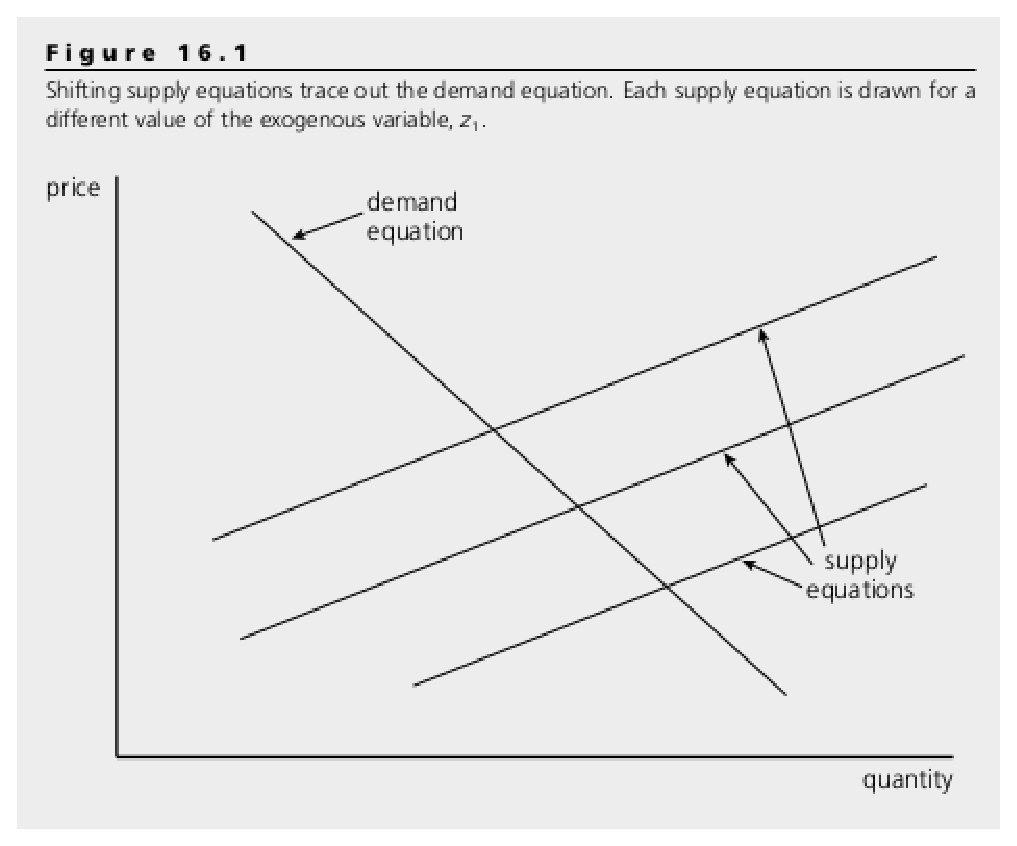
\includegraphics[scale = 0.5]{pictures/figure_16_1.eps}
\caption{Identifikace funkce poptávky pomocí $z_1$}
\label{figure_16_1}
\end{figure}

Rozšíření myšlenky identifikace na obecný případ modelu o dvou rovnicích je poměrně přímočaré. Uvažujme rovnice
\begin{equation}
y_1 = \beta_{10} + \alpha_1 y_2 + \pmb{z}_1 \pmb{\beta}_1 + u_1
\end{equation}
a
\begin{equation}
y_2 = \beta_{20} + \alpha_2 y_1 + \pmb{z}_2 \pmb{\beta}_2 + u_2,
\end{equation}
kde $y_1$ a $y_2$ jsou endogenní veličiny a $u_1$ a $u_2$ jsou strukturální chybové členy. Dále $\pmb{z}_1$ představuje vektor $k_1$ exogenních veličin figurujících v první rovnici, tj. $\pmb{z}_1 = (z_{11}, z_{12}, ..., z_{1 k_1})$. Podobně $\pmb{z}_2$ představuje vektor $k_2$ exogenních veličin obsažených v druhé rovnici, tj. $\pmb{z}_2 = (z_{21}, z_{22}, ..., z_{2 k_2})$. V mnoha případech se budou $\pmb{z}_1$ a $\pmb{z}_2$ překrývat. Nicméně je nutné, aby se tyto dva vektory nepřekrývaly zcela.\footnote{To by mimo jiné znamenalo, že nejsme schopni od sebe tyto rovnice odlišit.}

Rovnice (16.14) a (16.15) můžeme řešit s ohledem na $y_1$ a $y_2$, pokud je splněna podmínka $\alpha_2 \alpha_1 \ne 1$. Důkaz je ve své podstatě identický s příkladem jednoduchého modelu, který jsme představili v kapitole 16.2. Při splnění této podmínky existuje redukovaná forma pro $y_1$ i $y_2$.

\subsubsection{Podmínka identifikace}

První z SEM rovnic v modelu o dvou rovnicích je identifikovaná pouze tehdy a jen tehdy, pokud druhá rovnice obsahuje alespoň jednu exogenní veličinu (s nenulovým koeficientem), která není součástí této první rovnice. Tuto podmínku je možné otestovat pomocí $t$ popř. $F$ statistiky stejně, jak jsme si ukázali v kapitole 15.

\subsection{Odhad pomocí 2SLS}

Pokud je daná rovnice identifikovaná, můžeme ji odhadnout pomocí metody 2SLS. Pomocné veličiny se ``rekrutují'' z exogenních veličin, které figurují v některé z SEM rovnic.

\section{Simultánní modely s více než dvěma rovnicemi}

SEM mohou zahrnovat více než dvě rovnice. Obecná analýza těchto modelů je složitá a vyžaduje lineární algebru. V okamžiku, kdy je některá z rovnic identifikována, může být odhadnuta pomocí metody 2SLS.

\subsection{Model se třemi rovnicemi}

Pro ilustraci uvažujme následující systém rovnic.
\begin{equation}
y_1 = \alpha_{12}y_2 + \alpha_{13}y_3 + \beta_{11}z_1 + u_1
\end{equation}
\begin{equation}
y_2 = \alpha_{21} y_1 + \beta_{21}z_1 + \beta_{22}z_2 + \beta_{23}z_3 + u_2
\end{equation}
\begin{equation}
y_3 = \alpha_{32} y_2 + \beta_{31}z_1 + \beta_{32}z_2 + \beta_{33}z_3 + \beta_{34}z_4 + u_3
\end{equation}
Jako obvykle $y_g$ představuje endogenní veličiny a $z_j$ pak exogenní veličiny. První dolní index označuje číslo rovnice a druhý dolní index pak číslo veličiny. Parametry endogenních veličin označujeme jako $\alpha$ a parametry exogenních veličin jako $\beta$.

Kterou z výše uvedených rovnic můžeme odhadnout pomocí metody 2SLS? V případě obecného SEM s vícero rovnicemi je velmi problematické určit identifikovanou rovnici. Nicméně je mnohdy poměrně jednoduché určit neidentifikované rovnice. V případě výše uvedeného modelu je zřejmé, touto neidentifikovanou rovnicí je rovnice (16.18). Protože je v této rovnici obsažena každá exogenní veličina, nezůstává žádná exogenní veličina, kterou bychom mohli použít pro $y_2$ v roli pomocné veličiny. Proto nemůžeme konzistentně odhadnout parametry této rovnice. Rovnice (16.16) naproti tomu vypadá slibně - tato rovnice neobsahuje exogenní veličiny $z_2$, $z_3$ ani $z_4$, které tak mohou být použity jako pomocné veličiny. Ačkoliv (16.16) zahrnuje dvě endogenní veličiny, máme k dispozici tři exogenní veličiny, které můžeme použít jako pomocné veličiny pro $y_2$ a $y_3$. Rovnice (16.17) také vypadá slibně, protože exogenní veličinu $z_4$, která není v této rovnici obsažena, můžeme použít jako pomocnou veličinu pro jedinou endogenní veličinu $y_1$.

Obecná podmínka tedy zní, že pro danou rovnici musíme mít k dispozici alespoň tolik ``nevyužitých'' exogenních veličin jako je počet endogenních veličin zahrnutých v této rovnici. Tato podmínka je však nutná, nikoliv postačující pro identifikaci rovnice. Pokud by např. $\beta_{34} = 0$, pak $z_4$ nefiguruje v žádné ze tří rovnic simultánního modelu, což znamená, že není korelovaná s $y_1$, $y_2$ ani s $y_3$. Druhá rovnice tak není identifikována, protože $z_4$ nemůže být použita jako pomocná veličina pro $y_1$. To, zda-li je daná rovnice identifikována, tak záleží na hodnotách parametrů ostatních rovnic.

V souvislosti s identifikací rovnic se často setkáme s pojmy přeidentifikovaná rovnice (overidentified equation), právě identifikovaná rovnice (just identified equaiton) a neidentifikovaná rovnice (unidentified equaiton). Pojem přeidentifikovaná rovnice popisuje situaci, kdy je počet ``nevyužitých'' exogenních veličin vyšší než počet endogenních veličin zahrnutých do rovnice. V našem ilustrativním příkladě je tak rovnice (16.16) přeidentifikovanou rovnicí. Právě identifikovaná rovnice je pak rovnice, pro kterou je počet ``nevyužitých'' exogenních veličin roven endogenních veličin. Příkladem této rovnice je rovnice (16.17). V případě neidentifikované rovnice je pak počet ``nevyužitých'' exogenních veličin menší než počet endogenních veličin obsažených v rovnici. V našem případě se jedná o rovnici (16.18).

\subsection{Odhad}

Bez ohledu na počet rovnic v simultánním modelu je možné každou identifikovanou rovnici odhadnout pomocí metody 2SLS. Množinu potenciálních pomocných veličin představují všechny exogenní veličiny, které jsou zahrnuty v libovolné rovnici modelu. Testy pro endogenitu, heteroskedasticitu, autokorelaci a nadbytečnou identifikaci lze zkonstruovat způsobem popsaným v kapitole 15.

\section{Simultánní model a časové řady}

Mezi historicky první aplikace SEM patří modely popisující vývoj ekonomiky. Jako příklad uvažujme jednoduchý Keynesiánský model agregované poptávky ve tvaru
\begin{equation}
C_t = \beta_0 + \beta_1 (Y_t - T_t) + \beta_2 r_t + u_{t1}
\end{equation}
\begin{equation}
I_t = \gamma_0 + \gamma_1 r_t + u_{t2}
\end{equation}
\begin{equation}
Y_t \equiv C_t + I_t + G_t,
\end{equation}
kde $C_t$ představuje spotřebu, $Y_t$ příjem, $T_t$ daňové odvody, $r_t$ úrokovou sazbu, $I_t$ investice a $G_t$ vládní výdaje. Předpokládáme, že $t$ označuje rok.

První rovnice představuje funkci agregované spotřeby, která závisí na disponibilním příjmu $Y_t - T_t$, úrokové sazbě a strukturálním chybovém členu $u_{t1}$. Druhá rovnice představuje jednoduchou funkci investic. Poslední rovnice je identitou, která je dána metodikou národního účetnictví. Tato rovnice platí z definice a tudíž neobsahuje chybový člen. Rovnici (16.21) neodhadujeme, nicméně ji potřebuje pro úplnou definici modelu.

Protože je náš model definován třemi rovnicemi, musí se v něm vyskytovat také tři endogenní veličiny. Při pohledu na první dvě rovnice je patrné, že $C_t$ a $I_t$ jsou zamýšleny jako endogenní veličiny. Navíc, s ohledem na výše uvedenou účetní identitu, je $Y_t$ třetí endogenní veličinou. V rámci modelu pak předpokládáme, že $T_t$, $r_t$ a $G_t$ jsou exogenní veličiny a jsou tak nekorelované s $u_{t1}$ a $u_{t2}$.

Pokud je $r_t$ exogenní, můžeme (16.20) odhadnout pomocí OLS. Funkce spotřeby závisí na disponibilním příjmu $Y_t - T_t$, který je endogenní, protože $Y_t$ je endogenní. K dispozici však máme dvě exogenní veličiny $T_t$ a $G_t$. Tuto rovnici tak jsme schopni odhadnout pomocí 2SLS a pomocných proměnných $(T_t, G_t, r_t)$.

Problémem výše uvedeného SME je jeho statičnost. To se však dá snadno napravit zahrnutím zpožděných veličin. Např. rovnici (16.20) lze upravit na
\begin{equation}
I_t = \gamma_0 + \gamma_1 r_t + \gamma_2 Y_{t - 1} + u_{t2}
\end{equation}
Můžeme v tomto kontextu chápat $Y_{t-1}$ jako exogenní veličinu? Při splnění určitých předpokladů ohledně $u_{t2}$ ano. Nicméně obvykle nazýváme zpožděnou endogenní veličinu zahrnutou do simultánního modelu jako předvybranou veličinou (predetermined variable). Jestliže předpokládáme, že $u_{t2}$ je nekorelované se současnými exogenními veličiny a všemi minulými endogenními a exogenními veličinami, pak je $Y_{t-1}$ z definice nekorelované s $u_{t2}$. S ohledem na exogenitu $r_t$ tak můžeme (16.22) odhadnout pomocí OLS.

Pokud bychom přidali $C_{t-1}$ do (16.19), můžeme tuto zpožděnou veličinu považovat za exogenní za předpokladu, že je nekorelované s $u_{t1}$. Tím získáme následující rovnici.
\begin{equation}
C_t = \beta_0 + \beta_1 (Y_t - T_t) + \beta_2 r_t + \beta_3 C_{t - 1} + u_{t1}
\end{equation}
Protože je současný disponibilní příjem $(Y_t - T_t)$ je stále endogenní, musíme tuto rovnici odhadnout pomocí 2SLS s využitím pomocným veličin $(T_t, G_t, r_t, C_{t-1})$. Pokud je funkce investic dána (16.22), pak může být na list pomocných veličin přidána také veličina $I_{t-1}$.

Platnost klasické OLS a 2SLS metody pro účely určení konfidenčních intervalů, $t$ a $F$ testů závisí na předpokladu slabé závislosti. Bohužel makroekonomické veličiny velmi často tento předpoklad porušují. Terminologií kapitoly 11 je označujeme jako proces s jednotkovým kořenem. Dokonce i ve výběrech velkého rozsahu (nemluvě o výběrech malého rozsahu) jsou vlastnosti OLS a 2SLS odhadů procesů s jednotkovým kořenem komplikované a závisí na celé řadě předpokladů. Problém jednotkového kořene lze alespoň částečně vyřešit pomocí první diference podkladové časové řady. Nicméně je třeba si uvědomit, že po aplikaci diference se již jedná o jiný model.

Dalším praktickým problémem SEM může být nalezení vhodných pomocných veličin. Tento problém je obvykle snadněji řešitelný pro dezagregovaná data. Jako příklad uvažujme zpracovatelský průmysl, kde výstup jednoho odvětví může být použit jako pomocná veličina pro nabídkovou funkci druhého odvětví.

\section{Panelová data}

Uvažujme situaci, kdy se snažíme odhadnout funkci nabídky práce a funkci nabízené mzdy pro určitou skupinu lidí a určitý časový úsek. Kromě odhadu parametrů pro jednotlivé časové periody můžeme také pro jednotlivé rovnice uvažovat nepozorované veličiny. Např. pro nabídku práce můžeme uvažovat nepozorovanou hodnotu volného času, o které můžeme předpokládat, že je konstantní v čase.

Základní přístup při odhadu simultánního modelu nad panelovými daty zahrnuje dva kroky. Nejprve se pokusíme odstranit nepozorované veličiny (např. konstantní hodnotu volného času) pomocí první diference nebo jiné vhodné transformace. Následně najdeme vhodné pomocné veličiny pro endogenní veličiny zahrnutých v těchto transformovaných rovnicích. Pro ilustraci uvažujme model
\begin{equation}
y_{it1} = \alpha_1 y_{it2} + \pmb{z}_{it1} \pmb{\beta}_1 + a_{i1} + u_{it1}
\end{equation}
\begin{equation}
y_{it2} = \alpha_2 y_{it1} + \pmb{z}_{it2} \pmb{\beta}_2 + a_{i2} + u_{it2},
\end{equation}
kde $i$ označuje průřez (např. konkrétního jedince), $t$ označuje čas a $\pmb{z}_{it1} \pmb{\beta}_1$ popř. $\pmb{z}_{it2} \pmb{\beta}_2$ označují lineární kombinace exogenních nezávislých veličin v jednotlivých rovnicích. V obecném modelu mohou být nepozorované veličiny $a_{i1}$ a $a_{i2}$ korelované se všemi nezávislými veličinami. Nicméně předpokládáme, že idiosynkratické strukturální chybové členy $u_{it1}$ a $u_{it2}$ jsou nekorelované se $\pmb{z}$, což činí $\pmb{z}$ vektorem exogenních veličin. S výjimkou speciálních případů je pak $y_{it2}$ korelováno s $u_{it1}$ a $y_{it1}$ je korelováno s $u_{it2}$.

Předpokládejme, že chceme odhadnout rovnici (16.24). Tuto rovnici však nemůžeme odhadnout pomocí OLS, protože složený chybový člen $a_{i1} + u_{it1}$ je potenciálně korelovaný se všemi nezávislými veličinami. Proto aplikujeme první diferenci, čímž získáme
\begin{equation}
\Delta y_{it1} = \alpha_1 \Delta y_{it2} + \Delta \pmb{z}_{it1} \pmb{\beta}_1 + \Delta u_{it1}.
\end{equation}
Chybový člen v této rovnici je nekorelovaný s $\Delta \pmb{z}_{it1}$, což je dáno našimi výchozími předpoklady. Nicméně $\Delta y_{it2}$ a $\Delta u_{it1}$ jsou stále potenciálně korelované. Proto potřebujeme pomocnou veličinu pro $\Delta y_{it2}$. Pokud bychom aplikovali první diferenci také na (16.25), pak jsou přirozenými pomocnými veličinami pro $\Delta y_{it2}$ veličiny $\Delta \pmb{z}_{it2}$, které nejsou obsaženy v $\Delta \pmb{z}_{it1}$. Aby byl daný prvek $\Delta \pmb{z}_{it2}$ použitelný jako pomocná veličina, musí se měnit v čase. Pokud bych chtěli např. použít veličinu $\Delta exper_{it}$ (změna pracovní praxe v letech), zjistili bychom, že tato veličina není použitelná. Protože všichni jedinci v populaci pracují po celé zkoumané období, platí pro každého z nich v každém roce $\Delta exper_{it} = 1$. Je zřejmé, že takováto veličina je bezcenná.

Testování AR(1) potenciálně přítomné v $r_{it1} = \Delta u_{it1}$ je jednoduché. Nejprve pomocí 2SLS získáme odhad chybového členu $\hat{r}_{it1}$. Následně přidáme chybový člen zpožděný o jednu časovou periodu do původní rovnice, kterou opět odhadneme pomocí 2SLS; $\hat{r}_{it1}$ slouží jako pomocná veličina sebe sama. Autokorelaci lze pak otestovat pomocí obvyklé 2SLS $t$ statistiky aplikované na koeficient zpožděného chybového členu.
\chapter{Omezené závislé veličiny a korekce náhodného výběru}

Příkladem omezené závislé veličiny (limited dependent variable [LDV]) je binární závislá veličina. Obecně je omezená závislá veličina definována jako veličina, jejíž obor hodnot je zásadním způsobem omezen. Kromě veličin s taxativním oborem hodnot se jedná také o veličiny, které mohou nabývat hodnot pouze z určitého intervalu (např. pravděpodobnost vzniku pojistné události) nebo mohou z logiky věci nabývat pouze nezáporných hodnot (např. objem zemědělské produkce v určitém období, výše hodinové mzdy nebo počet návštěvníků výstavy).

Souvisejícím problémem je tzv. hraniční odezva (corner solution response). Např. mnoho rodin nepřispívá na charitu, a proto bude výše poskytnutých příspěvků pokrývat široký interval kladných hodnot se zvýšenou koncentrací bodě nula. Klasický lineární model pak predikuje pro řadu rodin namísto nulových záporné příspěvky na charitu.

V některých případech může být závislá proměnná omezena důsledkem toho, jak sbíráme a vyhodnocujeme data. Klasickým příkladem je stanovení určitého dolního či horního limitu při získávání informací o náhodném výběru (např. počet osob v domácnosti šest a více, měsíční příjem domácnosti do 20~000 CZK) nebo záměrné omezení výběru (např. omezení se pouze na zaměstnané osoby při zjišťování příjmového potenciálu jednotlivých osob). 

V řadě případů lze problém omezené závislé veličiny obejít pomocí vhodné transformace a použít tradiční OLS model. V některých případech je však třeba použít alternativním model.

\section{Logit a probit model pro binární závislou veličinu}

V případě binární závislé veličiny nás zajímá pravděpodobnostní model
\begin{equation}
P[y = 1 |x] = P[y = 1 | x_1, x_2, ..., x_k],
\end{equation}
pro jehož odhad lze použít logit popř. probit model.

\subsection{Specifikace logit a probit modelu}

Uvažujme model
\begin{equation}
P[y=1 | x] = G(\beta_0 + \beta_1 x_1 + ... + \beta_k x_k) = G(\beta_0 + x \beta),
\end{equation}
kde $G$ představuje funkci nabývající hodnot mezi nulou a jedničkou, tj. $0 < G(z) < 1$ pro všechny hodnoty $z$. V případě logit modelu má tato funkce tvar
\begin{equation}
G(z) = \frac{e^z}{1 + e^z} = \Lambda(z)
\end{equation}
a v případě probit modelu tvar
\begin{equation}
G(z) = \Phi(z) = \int_{-\infty}^{\infty}\phi(v)dv,
\end{equation}
kde $\phi(z) = \frac{1}{\sqrt{2 \pi}}e^{-\frac{z^2}{2}}$ představuje hustotu pravděpodobnosti standardního normálního rozdělení.

Logit a probit model lze odvodit na základě latentní veličiny $y^*$ definované jako
\begin{equation}
y^* = \beta_0 + x \beta + e, ~~~ y = 1[y^* > 0].
\end{equation}
Funkce $1[\cdot]$ je tzv. indikační funkcí, která nabývá hodnoty jedna, pokud je výraz v závorkách pravdivý a nula, pokud je výraz nepravdivý. Dále předpokládáme, že $e$ a $x$ jsou nezávislé a že $e$ sleduje standardní logistické nebo standardní normální rozdělení. V obou těchto případech je $e$ rozděleno symetricky kolem nuly, což implikuje $1 - G(-z) = G(z)$. Ekonomové zpravidla preferují předpoklad normality $e$, a proto se praxi častěji setkáváme s probit než s logit modelem.

S využitím (17.5) a $1 - G(-z) = G(z)$ tak lze $P[y = 1 | x]$ upravit do tvaru
\begin{multline}
P[y = 1 | x] = P[y^* > 0 | x] = P[e > -(\beta_0 + x \beta) | x]\\
= 1 - G[-\beta_0 + x\beta] = G(\beta_0 + x \beta),
\end{multline}
což odpovídá (17.2).

Stejně jako v klasickém lineární modelu je snahou odhadnout vliv $x_j$ na pravděpodobnost $P[y=1|x]$. To je však komplikováno nelinearitou $G(\cdot)$. Jestliže je $x_j$ alespoň přibližně spojitou veličinou, lze její dopad na $p(x) = P[y = 1 | x]$ získat pomocí parciální derivace
\begin{equation}
\frac{\partial p(x)}{\partial x_j} = g(\beta_0 + x \beta)\beta_j,
\end{equation}
kde $g(z) \equiv \frac{dG(z)}{dz}$. Protože $G$ je kumulativní distribuční funkce spojité náhodné veličiny, je $g$ hustotou pravděpodobnosti. V případě logit a probit modelu je $G$ striktně rostoucí, a proto $g(z) > 0$ pro všechna $z$. Dopad $x_j$ na $p(x)$ tak má vždy stejný směr jako $\beta_j$ bez ohledu na $x_j$. Je důležité si uvědomit, že ačkoliv nám stačí znalost znaménka $\beta_j$, abychom odhadli směr dopadu $x_j$ na $p(x)$, pro odhad jeho velikosti je třeba znát nejen velikost změny $x_j$, ale také celý vektor $x$ závislých veličin.

Ze vztahu (17.7) je také patrné, že relativní dopad  dvou nezávislých veličin $x_j$ a $x_h$ je $\frac{\beta_j}{\beta_h}$ a nezáleží tak na vektoru nezávislých veličin $x$. Jestliže je $g$ symetrické kolem nuly, je dopad $x_j$ na $p(x)$ největší pro $\beta_0 + x \beta = 0$.\footnote{Např. pro probit model, kde $g(z) = \phi(0)$, se jedná o $g(0) = \phi(0) = \frac{1}{\sqrt{2 \pi}} \approx 0.40$. V případě logit model se jedná o $z(0) = 0.25$.}

V případě, že je $x_1$ binární veličinou (a tudíž není možné aplikovat parciální derivaci), lze dopad změny $x_1$ z jedné na nulu (za předpokladu neměnnosti ostatních nezávislých veličin) kvantifikovat pomocí
\begin{equation}
G(\beta_0 + \beta_1 x_1 + \beta_2 x_2 + ... + \beta_k x_k) - G(\beta_0 + \beta_2 x_2 + ... + \beta_k x_k).
\end{equation}
Analogický postup lze aplikovat také na ostatní veličiny a to včetně spojitých veličin.

Základní model (17.2) lze snadno rozšířit pomocí transformací nezávislých veličin. Jako příklad uveďme
\begin{equation}
P[y = 1 | x] = G(\beta_0 + \beta_1 x_1 + \beta_2 x_1^2 + \beta_3 log(x_2) + \beta_4 x_3).
\end{equation}
Vztahy (17.7) popř. (17.8) je pak třeba upravit odpovídajícím způsobem.

\subsection{Metoda maximální věrohodnosti}

Vzhledem k nelinearitě $E[y|x]$ nelze pro odhad logit popř. probit modelu použít OLS methodu. Proto pro odhad parametrů těchto modelů použijeme tzv. metodu maximální věrohodnosti (maximum likelihood method). Protože je odhad na základě maximální věrohodnosti (maximum likelihood estimation [MLE]) založen na distribuci $y$ podmíněné vektorem nezávislých veličin $x$, je heteroskedasticita obsažená ve $var[y|x]$ automaticky zohledněna.

Pro odhad parametrů pomocí metody maximální věrohodnosti potřebujeme hustotu pravděpodobnosti $y_i$ pro daný vektor $x_i$, kterou lze vyjádřit jako
\begin{equation}
f(y|x_i; \beta) = [G(x_i \beta)]^y[1 - G(x_i\beta)]^{1-y}, ~~~ y = 0, 1,
\end{equation}
kde pro jednoduchost zahrneme průsečík do vektoru $x_i$. Aplikací logaritmu pak získáme tzv. logaritmickou funkci věrohodnosti (log-likelihood function)
\begin{equation}
\ell_i(\beta) = y_i log[G(x_i \beta)] + (1 - y_i)log[1 - G(x_i \beta)].
\end{equation}
Protože funkce $G$ nabývá hodnot z intervalu $(0, 1)$, je $\ell_i(\beta)$ definována pro všechny hodnoty $\beta$. Logaritmická věrohodnost (log-likelihood) pro náhodný výběr velikosti $n$ je pak definován jako
\begin{equation}
\mathscr{L}(\beta) = \sum_{i = 1}^n \ell_i(\beta).
\end{equation}
MLE odhad označovaný jako $\hat{\beta}$ je získán numerickou maximalizací $\mathscr{L}(\beta)$. Teorie MLE pro náhodný výběr pak implikuje, že při splnění velmi obecných předpokladů je takto získaný odhad konzistentní, asymptoticky normální a asymptoticky efektivní. Asymptotické směrodatné odchylky pro jednotlivá $\hat{\beta}_j$ lze vypočíst na základě relativně složitého vzorce, který je uveden v dodatku k této kapitole. S jejich pomocí lze zkonstruovat asymptotické $t$ testy a intervaly spolehlivosti stejně jako v případě klasického OLS modelu.

\subsection{Testování vícero lineárních omezení}

V následujícím textu se omezíme na testy významnosti. V případě, že lze odhadnout omezený i neomezený model, lze pro účely testování použít test založený na věrohodnostním poměru (likelihood ratio [LR]). Tento test je koncepčně shodný s $F$ testem pro lineární model. $F$ test měří nárůst součtu čtverce reziduí z titulu vynechání některých nezávislých veličin; LR test je založen na rozdílu logaritmických funkcí věrohodnosti neomezeného a omezeného modelu. LR statistika je definována jako
\begin{equation}
LR = 2(\mathscr{L}_{ur} - \mathscr{L}_r).
\end{equation}
Protože $\mathscr{L}_{ur} \ge \mathscr{L}_{r}$, je LR statistika vždy nezáporná a zpravidla striktně kladná. Vynásobení rozdílu $\mathscr{L}_{ur} - \mathscr{L}_r$ je zapotřebí k tomu, aby LR statistika při nulové hypotéze přibližně sledovala chi-kvadrát rozdělení s $q$ stupni volnosti, kde $q$ představuje počet nezávislých veličin odstraněných z původního modelu. Jinými slovy platí $LR \sim^a \chi_q^2$.

\subsection{Interpretace logit a probit modelu}

\subsubsection{Míra shody}

Pro ohodnocení logit popř. probit modelu můžeme použít míru shody označovanou jako správně predikované procento (precent correctly predicted). Binární prediktor $y_i$ definujeme rovný jedné, pokud je predikovaná pravděpodobnost větší nebo rovna 0.50, a rovný nule v opačném případě, tj. $\tilde{y}_i = 1$ pro $G(\hat{\beta}_0 + x_i \hat{\beta}) \ge 0.50$ a $\tilde{y}_i = 0$ pro $G(\hat{\beta}_0 + x_i \hat{\beta}) < 0.50$. Je zřejmé, že pro pár $(y_i, \tilde{y}_i)$ můžeme získat čtyři možné kombinace a to $(0, 0)$, $(1, 1)$, $(1, 0)$ a $(0, 1)$. Procento správných predikcí je dáno poměrem párů, kde $y_i = \tilde{y}_i$, ku všem párům.

Míra správně predikovatelného procenta však může být zavádějící. Např. v situaci, kdy pro 190 pozorování z celkového počtu 200 platí $y_i = 1$, je úspěšnost modelu $y = 1$ rovna 95\%. V praxi však často požadujeme alespoň určitou schopnost predikovat i méně pravděpodobné výsledky. Proto je vhodné spočítat procento správných predikcí pro obě hodnoty binární závislé veličiny.

Někteří také kritizují volbu 0.50 jako hraniční hodnoty a to zejména v případech, kdy je realizace jedné z hodnot závislé veličiny nepravděpodobná. Jestliže např. $\overline{y} = 0.08$ (tj. pouze 8\% úspěšnost v náhodném výběru), může se stát, že model nebude nikdy predikovat $y_i = 1$, protože jím odhadovaná pravděpodobnost nebude nikdy vyšší než 0.50. Jedním z řešení je tak použít hraniční hodnotu 0.08 namísto 0.50, tj. $\tilde{y}_i = 1$ pro $G(\hat{\beta}_0 + x_i \hat{\beta}) \ge 0.08$ a $\tilde{y}_i = 0$ pro $G(\hat{\beta}_0 + x_i \hat{\beta}) < 0.08$. Tento přístup sice zvýší počet predikovaných $\tilde{y}_i = 1$, ale zároveň se budeme dopouštět většího počtu chyb. Z tohoto důvodu může být míra správně predikovaného procenta dokonce horší než pro hraniční hodnotu 0.50.

Další možností je zvolit hraniční hodnotu tak, aby relativní počet $\tilde{y}_i = 1$ byl co nejblíže $\overline{y}$. Jinými slovy se snažíme odvodit hraniční hodnotu $0 < \tau < 1$, aby pro $\tilde{y} = 1$ kdy $G(\hat{\beta}_0 + x_i \hat{\beta}) \ge \tau$ platilo $\sum_{i = 1}^n \tilde{y}_i \approx \sum_{i = 1}^n y_i$.

Pro modely s binární závislou veličinou existují také nejrůznější pseudo $R^2$ ukazatele. Např. McFadden (1974) navrhuje míru $1 - \mathscr{L}_{ur} / \mathscr{L}_o$, kde $\mathscr{L}_{ur}$ je logaritmická funkce věrohodnosti odhadovaného modelu a $\mathscr{L}_o$ je logaritmická funkce věrohodnosti modelu, který zahrnuje pouze průsečík. Proč dává tato míra smysl? Platí, že $\mathscr{L}_{ur} / \mathscr{L}_o$ spadá do intervalu $(0, 1)$, a proto také takto definované pseudo $R^2$ nabývá hodnot z tohoto intervalu. Jestliže nezávislé veličiny nemají žádnou vysvětlující sílu, pak $\mathscr{L}_{ur} = \mathscr{L}_o$ a $1 - \mathscr{L}_{ur} / \mathscr{L}_o = 0$. V případě, kdy model velmi dobře popisuje realitu náhodného výběru, se $\mathscr{L}_{ur}$ blíží nule a $1 - \mathscr{L}_{ur} / \mathscr{L}_o \approx 1$. To odpovídá tradiční definici $R^2$.

Další alternativní pseudo $R^2$ ukazatel je bližší standardnímu $R^2$. Nechť jsou $\hat{y}_i = G(\hat{\beta}_0 + x_i \hat{\beta})$ pravděpodobnosti odhadované logit popř. probit modelem. Protože jsou tyto pravděpodobnosti zároveň odhadem $E[y_i | x]$, můžeme jednoduše vypočíst korelaci mezi $y_i$ a $\hat{y}_i$. To je v případě lineárního regresního modelu ekvivalentní ke klasickému výpočtu $R^2$. Takto získané pseudo $R^2$ je tedy přímo porovnatelné se standardním $R^2$.

\subsubsection{Vliv nezávislých veličin}

V praxi velmi často potřebujeme odhadnout vliv $x_j$ na pravděpodobnost $P[y = 1 | x]$. Jestliže je $x_j$ ``přibližně'' spojité, pak
\begin{equation}
\Delta \hat{P}[y = 1 | x] \approx [g(\hat{\beta}_0 + x \hat{\beta})\hat{\beta}_j]\Delta x_j
\end{equation}
pro ``dostatečně'' malé změny $x_j$. V porovnání s klasickým lineárním modelem je tedy v případě logit popř. probit modelu kvantifikace vlivu vysvětlující veličiny $x_j$ komplikovanější kvůli členu $g(\hat{\beta}_0 + x \hat{\beta})$, který závisí na vektoru nezávislých veličin $x$. V praxi často kvantifikuje vliv změny $x_j$ pro vektor $x$, který je reprezentován středními hodnotami nezávislých veličin, tj.
\begin{equation}
g(\hat{\beta}_0 + \overline{x} \hat{\beta}) = g(\hat{\beta}_0 + \hat{\beta}_1 \overline{x}_1 + \hat{\beta}_2 \overline{x}_2 + ... + \hat{\beta}_k \overline{x}_k).
\end{equation}
Tento přístup nazýváme parciálním efektem na průměr (partial effect at the average [PEA]). Problém může nastat v případě diskrétním nezávislých veličin, kdy průměr nemusí odpovídat žádné v reálu pozorované hodnotě.\footnote{Jako příklad takovéto nezávislé veličiny uvažujme pohlaví, které nabývá hodnoty 0, pokud se jedná o muže a hodnoty 1, pokud se jedná o ženu. Je zřejmě, že pokud budeme mít v náhodně vybraném vzorku jak muže tak ženy, pak průměrná hodnota této nezávislé veličiny nebude dávat smysl.} Další problém nastává, pokud nezávislá veličina figuruje jako vstup do nelineární funkce jako je např. přirozený logaritmus. Není totiž zřejmé, zda-li máme použít $\log(\overline{x}_j)$ nebo $\overline{\log(x_j)}$.

Alternativním přístupem je tzv. průměrný parciální efekt (average partial effect [APE]). Pokud je nezávislá veličina $x_j$ spojitá, pak je APE definován jako
\begin{equation}
\frac{1}{n}\sum_{i = 1}^n [g(\hat{\beta}_0 + x_j \hat{\beta})\hat{\beta}_j] = \hat{\beta}_j\Big[\frac{1}{n}\sum_{i = 1}^n [g(\hat{\beta}_0 + x_j \hat{\beta})\Big],
\end{equation}
kde $\frac{1}{n}\sum_{i = 1}^n [g(\hat{\beta}_0 + x_j \hat{\beta})$ funguje jako škálovací faktor.

Výše uvedené postupy spoléhaly na to, že je $x_j$ spojitá nezávislá veličina. V případě diskrétních nezávislých veličin je pro kvantifikaci změny z $c_j$ na $c_j + 1$ možné použít 
\begin{multline}
G[\hat{\beta}_0 + \hat{\beta}_1 \overline{x}_1 + ... + \hat{\beta}_{j - 1} \overline{x}_{j - 1} + \hat{\beta}_j (c_j + 1) + ... + \hat{\beta}_k \overline{x}_k]\\
- G[\hat{\beta}_0 + \hat{\beta}_1 \overline{x}_1 + ... + \hat{\beta}_{j - 1} \overline{x}_{j - 1} + \hat{\beta}_j c_j + ... + \hat{\beta}_k \overline{x}_k]
\end{multline}
v případě PEA a
\begin{multline}
\frac{1}{n}\sum_{i = 1}^n \Big(G[\hat{\beta}_0 + \hat{\beta}_1 x_{i1} + ... + \hat{\beta}_{ij - 1} x_{ij - 1} + \hat{\beta}_ij] (c_j + 1) + \hat{\beta}_k x_ik]\\
- G[\hat{\beta}_0 + \hat{\beta}_1 x_{i1} + ... + \hat{\beta}_{ij - 1} x_{ij - 1} + \hat{\beta}_ij] c_j + \hat{\beta}_k x_ik] \Big)
\end{multline}
v případě APE.

V případě, že na náhodném výběru kalibrujeme logit, probit i klasický lineární regresní model, je vhodné porovnat parciální vlivy jednotlivých nezávislých veličin napříč modely. Je důležité mít na paměti, že je třeba porovnávat parciální efekty a nikoliv přímo odhadnuté koeficienty. V případě logit a probit modelu je třeba koeficienty vynásobit škálovacím faktorem dle PEA popř. APE přístupu; v případě klasického lineárního regresního modelu je škálovací faktor implicitně roven jedné. Dále je třeba si uvědomit, že klasický lineární regresní model předpokládá konstantní efekt, kdežto v případě logit a probit modelu tento efekt závisí na úrovni nezávislých veličin. Ačkoliv to není pravidlo, parciální vlivy by měly být ve většině případů stejného řádu.

\subsubsection{Problémy logit a probit modelu}

Probit model předpokládá, že $e$ v (17.5) sleduje standardní normální rozdělení. Tento předpoklad však nemusí být v praxi splněn - pravděpodobnost $P[y=1|x]$ pak nelze popsat pomocí probit modelu. Někteří ekonometrové v tomto případě zdůrazňují nekonzistenci v odhadu $\beta_j$. To je však poněkud zavádějící poznámka, s výjimkou situace, kdy nás zajímá pouze směr parciálního efektu nezávislé veličiny $x_j$. Protože neznáme pravděpodobnost $P[y=1|x]$, nejsme schopni odhadnout velikost parciálního efektu, ani kdybychom měli k dispozici konzistentní odhad $\beta_j$.

Další problém logit a probit modelu souvisí s heteroskedasticitou. Jestliže $var[e|x]$ závisí na vektoru nezávislých veličin $x$, pak pravděpodobnost $P[y=1|x]$ nemá formu $G(\beta_0 + x \beta)$. Namísto toho by bylo třeba zvolit obecnější model. Takovéto modely však nejsou v praxi příliš používané, protože logit a probit modely ve většině případů fungují velmi dobře.

\section{Tobit model}

Důležitým příkladem omezené závislé veličiny je model s hraničním řešením. V takovémto modelu je závislá veličina ``přibližně'' spojitá a rovna nule pro netriviální část populace.\footnote{Jako příklad takovéto veličiny můžeme uvažovat částku, kterou daný jedinec měsíčně utratí za alkohol.}

Nechť $y$ představuje veličinu, která je spojitá na striktně kladném intervalu a která nabývá nulové hodnoty s nenulovou pravděpodobností. Nic nám nebrání použít klasický lineární model. Lineární model může být dobrou aproximací $E[y|x]$ zvláště pro $x_j$ v okolí střední hodnoty; nicméně lineární model může také predikovat záporné hodnoty. Také předpoklad, že nezávislá veličina má konstantní parciální efekt na $E[y|x]$ může být zavádějící. Protože $y$ je omezeno na striktně pozitivní interval se zvýšenou pravděpodobností v bodě nula, nemůže $y$ podmíněně sledovat normální rozdělení. Pro takovýto typ vysvětlující veličiny je proto vhodnější použít jiný typ modelu.

V případě Tobit modelu je latentní veličina $y^*$ definována jako
\begin{equation}
y^* = \beta_0 + x \beta + u, ~~~ u|x ~ N(0, \sigma^2)
\end{equation}
a výstup Tobit modelu pak jako
\begin{equation}
y = \max(0, y^*).
\end{equation}
Latentní veličina $y^*$ splňuje klasické předpoklady lineárního modelu, tj. sleduje normální homoskedasticitní rozdělení s lineárním podmíněnou střední hodnotou. Protože je $y^*$ normálně rozdělené, má pro striktně kladné hodnoty spojitou distribuci. Proto platí
\begin{multline}
P[y = 0 | x] = P[y^* < 0 | x] = P[y^* < 0 | x] = P[u < -x|\beta|x]\\
=P\Big[\frac{u}{\sigma} < -\frac{x\beta}{\sigma}|x\Big] = \Phi\Big(-\frac{x \beta}{\sigma}\Big) = 1 - \Phi\Big(\frac{x\beta}{\sigma}\Big),
\end{multline}
kde $\frac{u}{\sigma}$ sleduje standardní normální rozdělení a je nezávislé na vektoru $x$. S cílem zjednodušit zápis jsme průsečík zahrnuli do vektoru $x$. Jestliže je $(x_i, y_i)$ náhodným výběr z populace, pak je hustota pravděpodobnosti $y_i$ podmíněna vektor $x_i$ definována jako
\begin{equation}
\frac{1}{\sqrt{2 \pi} \sigma} e^{-\frac{(y - x_i \beta)^2}{2 \sigma^2}} = \frac{1}{\sigma}\phi\Big(\frac{y - x_i \beta}{\sigma}\Big)
\end{equation}
pro $y > 0$, popř. jako
\begin{equation}
P[y_i = 0 | x_i] = 1 - \Phi(\frac{x_i \beta}{\sigma})
\end{equation}
pro $y = 0$.

Z (17.21) a (17.22) pak lze odvodit logaritmickou funkci věrohodnosti pro jednotlivá pozorování ve tvaru
\begin{multline}
\ell_i(\beta, \sigma) = 1(y_i = 0) \log\Big[1 - \Phi\Big(\frac{x_i \beta}{\sigma}\Big)\Big]\\
+ 1(y_i > 0) \log\Big[\frac{1}{\sigma} \phi\Big(\frac{y_i - x_i \beta}{\sigma}\Big)\Big].
\end{multline}
Logaritmickou věrohodnost pro náhodný výběr velikosti $n$ lze získat součtem $\ell_i(\beta, \sigma)$ přes všechna $i$. Její numerickou maximalizací lze odhadnout hodnoty parametrů $\beta$ a $\sigma$. Standardní směrodatné odchylky těchto odhadů lze použít při konstrukci $t$ testů a konfidenčních intervalů. Vzorec pro jejich výpočet je však příliš složitý, a proto jej neuvádíme.

Testování vícenásobných omezení lze implementovat skrze Waldův test nebo pomocí věrohodnostního poměru stejně jako v případě logit a probit modelu.

\subsection{Interpretace Tobit modelu}

V Tobit modelu nás zajímají dvě střední hodnoty a to (a) $E[y|y > 0, x]$, kterou nazýváme podmíněnou střední hodnotou, protože je podmíněná $y > 0$ a (b) $E[y|x]$, která je poněkud nesprávně nazývána nepodmíněnou střední hodnotou.\footnote{Tato střední hodnota je pochopitelně podmíněna vektorem nezávislých veličin $x$. Proto je pojem ``nepodmíněná'' poněkud zavádějící.} Jestliže známe $E[y | y > 0, x]$, lze snadno vypočíst $E[y|x]$, protože
\begin{equation}
E[y|x] = P[y > 0 | x] E[y | y > 0, x] = \Phi\Big(\frac{x \beta}{\sigma}\Big)E[y | y > 0, x].
\end{equation}
Abychom získali $E[y|y > 0, x]$, využijeme skutečnosti, že pro $z \sim N(0, 1)$ platí $E[z | z > c] = \frac{\phi(c)}{1 - \Phi(c)}$. Platí tedy
\begin{multline}
E[y | y > 0, x] = x \beta + E[u | u > -x \beta] = x \beta + \sigma E\Big[\frac{u}{\sigma}| \frac{u}{\sigma} > -\frac{x\beta}{\sigma}\Big]\\
= x \beta + \sigma \frac{\phi\Big(\frac{x \beta}{\sigma}\Big)}{\Phi\Big(\frac{x \beta}{\sigma}\Big)},
\end{multline}
protože $\phi(-c) = \phi(c)$, $1 - \Phi(-c) = \Phi(c)$ a $\frac{u}{\sigma}$ sleduje standardní normální rozdělení nezávislé na vektoru $x$. Výše uvedené lze shrnout do
\begin{equation}
E[y|y>0, x] = x \beta + \sigma \lambda \Big(\frac{x \beta}{\sigma}\Big),
\end{equation}
kde $\lambda(c) = \frac{\phi(c)}{\Phi(c)}$ je tzv. inverzní Millsův poměr.

Rovnice (17.27) je důležitá. Ukazuje, že očekávaná hodnota $y$ podmíněná na $y > 0$ je rovna $x \beta$ plus striktně kladný člen, který je $\sigma$ krát inverzní Millsův poměr v bodě $\frac{x \beta}{\sigma}$. Tato rovnice také ilustruje, proč aplikace OLS pouze na pozorování, kde $y_i > 0$, nevede ke konzistentnímu odhadu vektoru koeficientů $\beta$. Inverzní Millsův poměr zde totiž hraje roli opomenuté nezávislé veličiny, která je korelována s vektorem $x$.

Kombinací (17.25) a (17.27) pak získáváme
\begin{equation}
E[y|x] = \Phi\Big(\frac{x \beta}{\sigma}\Big)\Big[x \beta + \sigma \lambda\Big(\frac{x \beta}{\sigma}\Big)\Big] = \Phi\Big(\frac{x \beta}{\sigma}\Big)x \beta + \sigma \phi\Big(\frac{x \beta}{\sigma}\Big),
\end{equation}
kde druhá část vyplývá ze skutečnosti $\Phi\Big(\frac{x \beta}{ \sigma}\Big) \lambda\Big(\frac{x \beta}{\sigma}\Big)$. Pokud tedy $y$ sleduje Tobit model, je $E[y|x]$ nelineární funkcí $x$ a $\beta$. Stojí za povšimnutí, že pravá strana rovnice (17.28) je kladná pro libovolné hodnoty $x$ a $\beta$, a proto je také $E[y|x]$ vždy kladné. Je také zřejmé, že parciální efekt nezávislé veličiny $x_j$ na $E[y|y>0,x]$ a $E[y|x]$ má stejný směr jako koeficient $\beta_j$, ale jeho výše závisí na všech vysvětlujících veličinách a všech parametrech Tobit modelu (a to včetně $\sigma$).

Pokud je $x_j$ spojitá veličina, pak lze parciální efekt kvantifikovat s pomocí derivace
\begin{equation}
\frac{\partial E[y|y>0, x]}{\partial x_j} = \beta_j + \beta_j \frac{d \lambda}{dc}\frac{x \beta}{\sigma}
\end{equation}
za předpokladu, že $x_j$ není funkcionálně spojeno s ostatními závislými veličinami. Derivací $\lambda(c) = \frac{\phi(c)}{\Phi(c)}$ a s využitím $\frac{d \Phi(c)}{dc} = \phi(c)$ a $\frac{d \phi}{d c} = -c \phi(c)$ lze dokázat, že $\frac{d \lambda}{dc} = - \lambda(c)[c + \lambda(c)]$. Proto
\begin{equation}
\frac{\partial E[y|y > 0, x]}{\partial x_j} = \beta_j\Big(1 - \lambda \frac{x \beta}{\sigma}\Big[\frac{x \beta}{\sigma} + \lambda \frac{x \beta}{\sigma}\Big]\Big).
\end{equation}
Lze dokázat, že faktor $\Big(1 - \lambda \frac{x \beta}{\sigma}\Big[\frac{x \beta}{\sigma} + \lambda \frac{x \beta}{\sigma}\Big]\Big)$ spadá do intervalu $(0, 1)$. V praxi lze (17.30)  odhadnout pomocí MLE odhadů $\beta_j$ a $\sigma$. Stejně jako v případě logit a probit modelů je třeba zvolit hodnoty pro vektor nezávislých veličin $x$. Pro tento účel se nejčastěji používá vektor jejich středních hodnot.

Jestliže je $x_j$ binární veličinou, pak lze získat parciální efekt jako rozdíl $E[y|y > 0, x]$ pro $x_j = 1$ a $x_j = 0$. Parciální efekt obecné diskrétní veličiny lze určit analogicky.

S pomocí (17.28) lze získat parciální efekt spojité veličiny $x_j$ na $E[y|x]$. Tato derivace bere v potaz skutečnost, že lidé ``začínající'' v $y = 0$ si mohou zvolit $y > 0$, pokud se $x_j$ změní.
\begin{equation}
\frac{\partial E[y|x]}{\partial x_j} = \frac{\partial P[y > 0 | x]}{\partial x_j} E[y | y > 0, x] + P[y > 0 | x] \frac{\partial E[y | y > 0, x]}{\partial x_j}.
\end{equation}
Protože $P[y > 0 | x] = \Phi\Big(\frac{x \beta}{\sigma}\Big)$, pak
\begin{equation}
\frac{\partial P[y > 0 | x]}{\partial x_j} = \frac{\beta_j}{\sigma} \Phi\Big(\frac{x \beta}{\sigma}\Big).
\end{equation}
Tato rovnice nám umožňuje porovnat OLS a Tobit odhady.

Stejně jako v logit a probit modelu také v Tobit modelu lze škálovací faktor $\Phi\Big(\frac{x \beta}{\sigma}\Big)$ kvantifikovat dvěma způsoby - pomocí PEA a APE přístupu. V PEA přístupu má tento faktor podobu $\Phi\Big(\frac{\overline{x}\hat{\beta}}{\hat{\sigma}}\Big)$ a případě APE pak podobu $\frac{1}{n}\sum_{i = 1}^n \Phi\Big(\frac{x_i \hat{\beta}}{\hat{\sigma}}\Big)$. V obou případech spadají škálovací faktory do intervalu $(0, 1)$, protože $0 < \Phi\Big(\frac{x \hat{\beta}}{\hat{\sigma}}\Big) < 1$ pro libovolné hodnoty nezávislých veličin. Protože $\hat{P}[y_i > 0 | x_i] = \Phi\Big(\frac{x_i \hat{\beta}}{\hat{\sigma}}\Big)$, je PEA i APE škálovací faktor blízký jedné, pokud pouze omezené množství pozorování $y_i = 0$. V případě, že všechna pozorování jsou větší než nula, tj. $y_i > 0$ pro všechna $i$, jsou OLS a Tobit odhady identické.

Bohužel pro diskrétní veličiny není srovnání OLS a Tobit modelu stejně přímočaré jako pro spojité veličiny. V případě Tobit modelu je vhodné kvantifikovat parciální efekt skrze rozdíl dvou $E[y | x]$ pro odlišné hodnoty uvažované nezávislé veličiny. $E[y | x]$ lze vypočíst dle (17.25). Tento postup lze aplikovat jak pro EPA tak pro APE varianty odhadů. Stejný přístup jsem aplikovali také v případě logit a probit modelu.

\subsection{Problémy Tobit modelu}

Tobit model a konkrétně pak rovnice (17.27) a (17.28) závisí na předpokladu normality a homoskedasticity latentního modelu (17.19). V případě, že tyto předpoklady nejsou splněny, je velmi komplikované Tobit model správně interpretovat. Nicméně v případě mírného odchýlení se od těchto předpokladů bude nejspíše Tobit model stále poskytovat dobrý odhad parciálních efektů na $E[y|x]$.

Jedním z významných omezení Tobit modelu je skutečnost, že $E[y|y > 0]$ je úzce provázána s pravděpodobností $P[y > 0]$. To je patrné z (17.30) a (17.32). Konkrétně vliv $x_j$ na $E[y|y > 0, x]$ a $P[y > 0 | x]$ je proporcionální $\beta_j$ a škálovací faktory násobící $\beta_j$ jsou kladné a závisí na vektoru $x$ pouze skrze $\frac{x \beta}{\sigma}$. Pro ilustraci uvažujme  vztah mezi pokrytím životním pojištění a věkem. Pravděpodobnost sjednání pojištění je nižší u mladých lidí, a proto $P[y > 0]$ roste s věkem. Podmíněně na sjednání životního pojištění však hodnota pojistné smlouvy s věkem klesá, protože se pojištění ke konci života stává méně důležité. Tento vztah však není možné podchytit pomocí Tobit modelu.

Jedním ze způsobů, jak neformálně zhodnotit, zda-li je Tobit model vhodným pro daný problém, je odhadnout probit model, kde binární závislá veličina $w$ je rovna jedné, jestliže $y > 0$, popř. rovna nule, jestliže $y = 0$. Pak dle (17.23) sleduje $w$ probit model, kde koeficient pro $x_j$  je $\gamma_j = \frac{\beta_j}{\sigma}$. Tímto způsobem můžeme odhadnout poměr $\beta_j$ ku $\sigma$ pro každé $j$. Jestliže je použití Tobit modelu vhodné, pak $\hat{\gamma}_j$ by mělo být ``blízké'' $\frac{\hat{\beta}_j}{\hat{\sigma}}$, kde $\hat{\beta}_j$ a $\hat{\sigma}$ jsou odhadnuty z Tobit modelu. Tyto odhady však nebudou nikdy identické. Nicméně je možné se soustředit na určité indikace, které signalizují možné problémy. Např. je-li $\hat{\gamma}_j$ významné a záporné, avšak $\hat{\beta}$ je kladné, nemusí být použití Tobit modelu vhodné. Stejně tak možný problém indikuje příliš ``velký'' rozdíl mezi $|\hat{\beta}_j / \hat{\sigma}|$ a $|\hat{\gamma}_j|$. Pokud dojdeme k závěru, že použití Tobit modelu není vhodné, je možné použít alternativní modely jako je např. prahový model (hurdle model) nebo dvousložkový model (two-part model). Tyto modely však přesahují záběr knihy.

\section{Poissonův model}

Dalším příkladem nezáporné závislé veličiny je veličina, která vyjadřuje počet. Takovouto náhodnou veličinu je možné modelovat pomocí exponenciální funkce
\begin{equation}
E[y| x_1, x_2, ..., x_k] = e^{\beta_0 + \beta_1 x_1 + ... + \beta_k x_k}.
\end{equation}
Protože $exp(\bullet)$ je vždy kladné, je také $E[y|x]$ vždy kladné. Zlogaritmováním pak získáme
\begin{equation}
\log(E[y|x_1, x_2, ..., x_k]) = \beta_0 + \beta_1 x_1 + ... + \beta_k x_k.
\end{equation}
Připomeňme si, že $100 \beta_j$ přibližně vyjadřuje procentní změnu v $E[y|x]$ pro jednotkovou změnu $x_j$. Pokud tuto změnu chceme vyjádřit přesněji, je třeba použít
\begin{equation}
\frac{e^{\beta_0 + \beta_1 x_1 + ... + \beta_j x_j^1 + ... + \beta_k x_k}}{e^{\beta_0 + \beta_1 x_1 + ... + \beta_j x_j^0 + ... + \beta_k x_k}} - 1
\end{equation}

Protože (17.33) není lineární funkcí ve svých parametrech, nemůžeme na odhad Poissonova modelu použít OLS metodu. Pro tento účel použijeme metodu maximální věrohodnosti a příbuznou metodu kvazimaximální věrohodnosti.

Veličina, která vyjadřuje počet, nemůže ze své definice sledovat normální rozdělení. Namísto normálního rozdělení tak použijeme Poissonovo rozdělení. Poissonovo rozdělení je zcela definováno střední hodnotou $E[y|x]$. Předpokládejme, že tuto střední hodnotu lze popsat pomocí modelu (17.33), jehož zápis pro účely následujícího textu zkrátíme do podoby $E[y|x] = e^{x\beta}$. Pravděpodobnost, že $y$ je rovno $h$ podmíněně na $x$ je pak
\begin{equation}
P[y = h | x] = e^{-e^{x\beta}}\frac{\Big(e^{x\beta}\Big)^h}{h!}.
\end{equation}
Toto pravděpodobnostní rozdělení, které je základem pro Poissonův regresní model, nám umožňuje najít podmíněnou pravděpodobnost pro libovolné hodnoty nezávislých veličin.

Pro náhodný výběr $\{(x_i, y_i): i = 1, 2, ..., n\}$ definujeme logaritmickou věrohodnostní funkci jako
\begin{equation}
\mathscr{L}(\beta) = \sum_{i = 1}^n \ell_i(\beta) = \sum_{i = 1}^n \Big(y_i x_i \beta - e(x_i \beta) \Big),
\end{equation}
kde jsme vynechali konstantní člen $-\log(y_i!)$. Optimální hodnotu vektoru $\beta$ pak získáme numerickou maximalizací (17.37).

Stejně jako v případě logit, probit a Tobit modelu nelze přímo srovnat odhadnuté koeficienty Poissonova modelu s koeficienty OLS modelu. Pokud jsou předpoklady (17.33) splněny lze pro ``přibližně'' spojitou závislou veličinu Poissonova modelu odhadnout parciální efekt s pomocí
\begin{equation}
\frac{\partial E[y | x_1, x_2, ..., x_k]}{\partial x_j} = e^{\beta_0 + \beta_1 x_1 + ... + \beta_k x_k} \beta_j.
\end{equation}
Jestliže regresní koeficient OLS modelu nezávislé veličiny $x_j$ označíme jako $\gamma_j$, pak lze $\gamma_j$ porovnat s průměrným parciálním efektem. Stejně jako v předchozích případech tento průměrný parciální efekt existuje v EPA a APE. V případě APE přístupu je zajímavé, že $\frac{1}{n}\sum_{i = 1}^n e^{\hat{\beta}_0 + \hat{\beta}_1 x_{i1} + ... + \hat{\beta}_1 x_{ik}} = \frac{1}{n} \sum_{i = 1}^n \hat{y}_i = \overline{y}$. Pro je pro ``přibližně'' spojitou veličinu nejjednodušší porovnat $\hat{\gamma}_j$ s $\overline{y}\hat{\beta}_j$.

Ačkoliv je Poissonův model přirozenou volbou pro závislé veličiny, které vyjadřují počet, je tento model v řadě případů příliš omezující. Např. všechny pravděpodobnosti a vyšší momenty Poissonova pravděpodobnostního rozdělení jsou definovány střední hodnotou. Konkrétně platí
\begin{equation}
var[y|x] = E[y|x],
\end{equation}
což v řadě reálných případů není splněno. Nicméně Poissonův model je velmi robustní - bez ohledu na to, zda je splněn předpoklad Poissonova rozdělení, získáme konzistentní a asymptoticky normální odhady koeficientů $\beta_j$.\footnote{To je analogické s OLS odhady, které jsou taktéž konzistentní a asymptoticky normální, i když není splněn předpoklad normality.}

Jestliže nelze předpokládat splnění předpokladu Poissonova rozdělení, můžeme pro odhad modelu použít metodu kvazimaximální věrohodnosti (quasi-maximum likelihood estimation [QMLE]). Pokud předpoklad (17.39) není splněn, je třeba upravit chybový člen modelu. Nejjednodušší způsob úpravy je založen na předpokladu, že rozptyl je násobek střední hodnoty, tj.
\begin{equation}
var[y|x] = \sigma^2 E[y|x],
\end{equation}
kde $\sigma^2 > 0$ je neznámý parametr a obvykle platí $\sigma^2 > 1$.

Nechť $\hat{\beta}_j$ označuje Poisson QMLE a definujme rezidua jako $\hat{u}_i = y_i - \hat{y}_i$, kde $\hat{y}_i = e^{\hat{\beta}_0 + \hat{\beta}_1 x_{i1} + ... + \hat{\beta}_k x_{ik}}$. Konzistentní funkce odhadu $\sigma^2$ je $\frac{1}{n - k - 1} \sum_{j = 1}^n \frac{\hat{u}^2_i}{\hat{y}_i}$, kde jmenovatel $\hat{y}_i$ představuje ``vhodnou'' úpravu o heteroskedasticitu. Na závěr vynásobíme směrodatné odchylky odhadů Poissonova modelu parametrem $\hat{\sigma}$.

Za předpokladu splnění Poissonova rozdělení je možné testovat vícero lineárních omezení pomocí testu založeném na věrohodnostním poměru (17.13) stejně jako v případě logit / probit modelu. Při $q$ vylučovacích omezeních (tj. nulové hypotéze o statisticky nevýznamném regresním parametru) sleduje příslušná statistika přibližně $\chi^2_q$ rozdělení. Při méně restriktivním předpokladu (17.40) je třeba (17.13) vydělit $\hat{\sigma}^2$ z neomezeného modelu.

\section{Cenzurované a omezené regresní modely}

V případě, že při sběru dat byla závislá veličina omezena zdola nebo shora určitou hodnotou, používáme tzv. cenzurovaný regresní model (censored regression model). Omezený regresní model (truncated regression model) pak použijeme v případě populaci omezíme na základě závislé veličiny $y$ tím, že např. vyloučíme všechny domácnosti s ročním příjmem nad 10 miliónů korun.

\subsection{Cenzurovaný regresní model}

Předpokládejme, že $y$ sleduje klasický lineární model
\begin{equation}
y_i = \beta_0 + x_i \beta + u_i, ~~~ u_i|x_i, ~ c \sim N(0, \sigma^2.)
\end{equation}
Nicméně namísto $y_i$ máme k dispozici pouze informace o cenzurované hodnotě $w_i$, která je definována jako
\begin{equation}
w_i = \min(y_i, c_i),
\end{equation}
kde $c_i$ může být konstantní popř. být funkcí nezávislých veličin.

Vzhledem k ``cenzuře'' závislé veličiny není možné získat odhady modelu pomocí OLS - tyto odhady by totiž byly zkreslené. Proto, stejně jako v případě předchozích modelů, je třeba použít metodu maximální věrohodnosti. Za tímto účelem potřebujeme znát hustotu pravděpodobnosti pro $w_i$ podmíněnou $(x_i, c_i)$. Pro necenzurovaná pozorování $w_i = y_i$ je tato hustota pravděpodobnosti stejná jako pro $y_i$, tj. $N(x_i\beta, \sigma^2)$. Pro cenzurované hodnoty je pak tato funkce definována jako
\begin{equation}
P[w_i = c_i|x_i] = P[y_i \ge c_i | x_i] = P[u_i \ge c_i - x_i \beta] = 1 - \Phi\Big[\frac{c_i - x_i \beta}{\sigma}\Big].
\end{equation}
Kombinací těchto dvou hustot pravděpodobnosti pak získáváme
\begin{equation}
\begin{split}
f(w|x_i, c_i) & = 1 - \Phi\Big(\frac{c_i - x_i \beta}{\sigma}\Big), \quad w = c_i,\\
 & = \frac{1}{\sigma} \phi\Big(\frac{w - x_i \beta}{\sigma}\Big), \quad w < c_i.
\end{split}
\end{equation}
Logaritmickou věrohodnost lze vypočíst tak, že zlogaritmujeme hustotu pravděpodobnosti pro každé pozorování $i$. Maximalizací součtu přes všechna pozorování $i$ pak získáme optimální odhady vektoru $\beta$ a $\sigma$.

Regresní koeficient $\beta_j$ cenzurovaného modelu lze na rozdíl od předchozích modelů přímo porovnat s OLS odhady. To je dáno tím, že (17.41) a (17.42) představují lineární model.

Důležitou aplikací cenzurovaného regresního modelu je tzv. durační analýzu. Durací rozumíme veličinu, která měří čas, jenž uplyne do realizace určité události. Při durační analýze často aplikujeme logaritmus na závislou veličinu, což znamená, že musí logaritmus aplikovat také na prahovou hodnotu $c_i$. Regresní koeficienty jsou pak interpretovány jako procentní změna.

Pokud nejsou splněny některé z předpokladů cenzurovaného modelu, tj. pokud chybový člen vykazuje známky heteroskedasticity nebo nesleduje normální rozdělení, pak jsou MLE odhady nekonzistentní. Proto je cenzůra dat poměrně potenciálně problematická - při OLS může chybový člen trpět heteroskedasticitou a nemít normální rozdělení, a přesto budou odhady konzistentní.

\subsection{Omezený regresní model}

V případě omezeného regresního modelu nebereme v potaz celou populaci, ale pouze její část. Typickým příkladem je např. výzkum veřejného mínění, který se omezuje pouze na určitou věkovou kategorii. V tomto případě je porušeno pravidlo náhodného výběru. I když jsou výsledky výzkumu založené na OLS metodě relevantní pro danou věkovou kategorii, nelze je zobecňovat na celou populaci.

Uvažujme klasický lineární model
\begin{equation}
y = \beta_0 + x \beta + u, \quad u|x \sim N(0, \sigma^2).
\end{equation}
Předpokládejme, že je porušen předpoklad MLR.2 o náhodném výběru. Konkrétně předpokládejme, že náhodné pozorování $(x_i, y_i)$ je k dispozici pouze v případě, že $y_i \le c_i$, kde $c_i$ je prahová hodnota závislá na $x_i$. Stejně jako v předchozích případech potřebujeme podmíněnou funkci hustoty pro $y_i$. Ta je definována jako
\begin{equation}
g(y|x_i, c_i) = \frac{f(y|x_i \beta, \sigma^2)}{F(c_i | x_i \beta, \sigma^2)}, \quad y \le c_i,
\end{equation}
kde $f(y|x_i \beta, \sigma^2)$ označuje hustotu pravděpodobnosti normálního rozdělení se střední hodnotou $\beta_0 + x_i \beta$ a rozptylem $\sigma^2$ a $F(c_i | x_i \beta, \sigma^2)$ je hodnota odpovídající kumulativní pravděpodobnostní funkci v bodě $c_i$. Rovnice tedy přeškáluje hustotu pravděpodobnosti tím, že ji vydělíme plochou $f(\bullet | x_i \beta, \sigma^2)$ nalevo od $c_i$.

Pokud zlogaritmujeme (17.46), sečteme přes všechna $i$ a maximalizujeme s ohledem na $\beta$ a $\sigma^2$, získáme odhady regresních parametrů pomocí metody maximální věrohodnosti. Stejně jako v případě předchozích modelů lze standardním způsobem konstruovat konfidenční intervaly, testovat jednoduché hypotézy pomocí $t$ statistiky  nebo vícenásobné vylučovací hypotézy pomocí LR statistiky. Stejně jako v případě cenzurovaného modelu platí, že pokud nejsou splněny předpoklady homoskedasticity a normality, jsou odhadnuté regresní parametry zkreslené a nekonzistentní.

\section{Neúplný náhodný výběr}

Velice často se stává, že při výzkumu nejsou respondenti schopni zodpovědět některou z otázek. Výsledkem pak je neúplný set odpovědí. Protože nejsme schopni tato pozorování přímo použít pro odhad regresního modelu, nabízí se otázka, zda-li by jejich ignorování mělo za následek zkreslení OLS odhadů. S dalším podobným příkladem se můžeme setkat u panelových dat, kdy pro daného jedince máme k dispozici data např. po dobu dvou let, přičemž třetí rok již tento jedinec není součástí výběru.

\subsection{OLS a náhodný výběr}

Uvažujme populační model
\begin{equation}
y = \beta_0 + \beta_1 x_1 + ... + \beta_k x_k + u, \quad E[u | x_1, x_2, ..., x_k] = 0
\end{equation}
a zkrácený zápis tohoto modelu pro náhodné pozorování
\begin{equation}
y_i = x_i \beta + u_i.
\end{equation}
Nechť $n$ představuje velikost náhodného výběru z dané populace. Pokud pro každé náhodné pozorování $i$ máme k dispozici $y_i$ a všechna $x_{ij}$, můžeme použít OLS metodu pro odhadu modelu. Předpokládejme však, že pro některá pozorování toto není splněno. Definujme výběrový indikátor $s_i$, kde $s_i = 1$, pokud je předpoklad splněn a $s_i = 0$, pokud splněn není. Model (17.48) pak můžeme přepsat do tvaru
\begin{equation}
s_i y_i = s_i x_i \beta + s_i u_i.
\end{equation}
Tento model odpovídá situaci, pokud bychom model (17.48) aplikovala pouze na ta pozorování, pro která $s_i = 1$.

Z kapitoly 5 víme, že OLS odhady modelu (17.49) jsou konzistentní, pokud má chybový člen nulovou střední hodnotu a je nekorelovaný se všemi nezávislými veličinami, tj.
\begin{equation}
E[su] = 0
\end{equation}
a
\begin{equation}
E[(sx_j)(su)] = E[sx_ju] = 0,
\end{equation}
kde jsme nezávislou veličinu $x_j$ předefinovali na $s x_j$.

Klíčovým předpokladem pro nezkreslenost odhadu je $E[su | x x_1, ..., s x_k] = 0$. Jako obvykle se jedná o silnější předpoklad, než jaký je zapotřebí pro jeho konzistentnost.

Jestliže je $s$ funkcí nezávislých veličin, pak $s x_j$ je funkcí $x_1, x_2, ..., x_k$. Na základě předpokladu, který je součástí (17.47), je $s x_j$ také nekorelované s $u$. Ve skutečnosti platí $E[su|s x_1, ..., sx_k] = s E[u|sx_1, ..., s x_k] = 0$. To je příklad exogenního náhodného výběru, kde $x_i = 1$ je určeno pouze $x_{i1}, x_{i2}, ..., x_{ik}$.

Pokud je výběr zcela náhodný ve smyslu, že $s_i$ je nezávislé na $(x_i, u_i)$, pak $E[s x_j u] = E[s]E[x_j u] = 0$, protože dle (17.47)$E[x_ju] = 0$. Proto, pokud z náhodného výběru náhodně vyloučíme některá pozorování, jsou OLS odhady stále nezkreslené a konzistentní.

Příkladem, kdy jsou OLS odhady založené na náhodném výběru nekonzistentní, jsou tzv. omezené výběry (truncated sample). Jedná se např. o situaci, kdy $s_i = 1$ pro $u_i \le c_i - x_i \beta$. Protože $s_i$ přímo závisí na $u_i$, $s_i$ a $u_i$ nejsou nekorelované a to ani podmíněně na $x_i$. To vysvětluje, proč jsou OLS odhady na takovémto výběru nekonzistentní.

Lze dokázat, že pokud je výběr funkcí exogenních veličin, je odhad nelineárního modelu pomocí metody maximální věrohodnosti (jako např. logit a  probit modelu) konzistentní, asymptoticky normální a že směrodatné odchylky a standardní testovací statistiky jsou platné.

\subsection{Náhodné omezení výběru}

O náhodném omezení výběru (incidental truncation) hovoříme v případě, kdy pozorujeme $y$ pouze pro podmnožinu populace. Pravidlo výběru přitom nezávisí přímo na hodnotě $y$. Obvyklý přístup k náhodnému omezení výběru je přidání explicitní výběrové rovnice do populačního modelu
\begin{gather}
y = x \beta + u, \quad E[u|x] = 0\\
s = 1[z \gamma + v \ge 0],
\end{gather}
kde $s = 1$, pokud pozorujeme $y$, a $s = 0$ v opačném případě. Předpokládáme, že prvky vektorů $x$ a $z$ jsme schopni vždy pozorovat a že $x \beta = \beta_0 + \beta_1 x_1 + ... + \beta_k x_k$ a $z \gamma = \gamma_0 + \gamma_1 z_1 + ... + \gamma_m z_m$.

Předmětem našeho zájmu je (17.52) a vektor $\beta$ můžeme odhadnout pomocí OLS za předpokladu náhodného výběru. Výběrová podmínka (17.53) závisí na vektoru pozorovaných veličin $z$ a nepozorované chybě $v$. Standardním předpokladem je exogenita veličiny $z$, tj.
\begin{equation}
E[u |x,z] = 0.
\end{equation}
Aby níže popsaná metoda fungovala, je zapotřebí, aby vektor $x$ byl striktní podmnožinou $z$, tj. aby libovolné $x_j$ bylo podmnožinou $z$ a zároveň aby existovaly prvky $z$, které nejsou obsaženy v $x$.

Předpokládáme, že chybový člen $v$ je nezávislý na $z$ (a tím pádem také na $x$). Dále předpokládáme, že chybový člen $v$ sleduje standardní normální rozdělení. Je zřejmé, že korelace mezi $u$ a $v$ vede k problémům s náhodným výběrem. Pro ilustraci uvažujme, že $(u, v)$ je nezávislé na $z$. Střední hodnota (17.52) podmíněná $z$ a $v$ a s využitím skutečnosti, že $x$ je podmnožinou $z$, je
\begin{equation}
E[y|z, v] = x \beta + E[u | z, v] = x \beta + E[u | v],
\end{equation}
kde $E[u | z, v] = E[u|v]$, protože $(u, v)$ jsou nezávislé na $z$. Jestliže $u$ a $v$ jsou sdruženě normální s nulovou střední hodnotou, pak $E[u|v] = \rho v$ pro vhodně zvolené $\rho$. Proto
\begin{equation}
E[y|z, v] = x \beta + \rho v.
\end{equation}
I když nepozorujeme $v$, můžeme tuto rovnici použít pro výpočet $E[y|z,s]$ a následně zúžit pro $s = 1$. Nejprve tedy uvažujeme
\begin{equation}
E[y|z,s] = x \beta + \rho E[v|z,s].
\end{equation}
Protože $s$ a $y$ jsou propojeny skrze (17.53) a protože $v$ sleduje normální rozdělení, lze dokázat, že $E[y|z,s]$ je Millsův inverzní poměr pro $s = 1$, tj.
\begin{equation}
E[y|z, s = 1] = x \beta + \rho \lambda (z \gamma).
\end{equation}
Připomeňme si, že naším primárním cílem je odhad vektoru $\beta$. Výše uvedená rovnice nám říká, že to je v případě omezeného výběru možné pouze, pokud přidáme člen $\lambda(z \gamma)$ jako dodatečnou nezávislou veličinu. Jestliže $\rho = 0$, pak můžeme $\lambda(z \gamma)$ vypustit a metoda OLS vede ke konzistentnímu odhadu vektoru $\beta$. Protože neznáme $\gamma$, nemůžeme kvantifikovat $\lambda (z_i \gamma)$ pro každé $i$. Nicméně díky výše uvedeným předpokladům platí
\begin{equation}
P[s = 1 | z] = \Phi(z \gamma).
\end{equation}
Proto můžeme odhadnout $\gamma$ pomocí probit modelu $s_i$ na $z_i$, kde využijeme celý náhodný výběr. Na závěr pak odhadneme $\beta$. Následující text shrnuje krok za krokem tuto tzv. Heckitovu metodu.

\begin{enumerate}
\item S využitím všech $n$ pozorování odhadneme probit model $s_i$ na $z_i$, čímž získáme odhad vektoru $\hat{\gamma}$.
\item Vypočteme Millsův inverzní poměr $\hat{\lambda}_i = \lambda(z_i \hat{\gamma})$ pro všechna $i$.\footnote{Ve skutečnosti potřebujeme výpočet pouze pro ta $i$, pro která $s_i = 1$.}
\item S využitím omezeného výběru (tj. pro pozorování pro která $s_i = 1$) definujeme regresní model
\begin{equation}
y_i = x_i \beta + \hat{\lambda}_i \rho.
\end{equation}
Odhad $\hat{\beta}$ je konzistentní a přibližně normálně rozdělený.
\end{enumerate}

Jednoduchý test na chybějící nezávislou veličinu je možné založit na (17.60). Konkrétně lze použít obvyklou $t$ statistiku k tomu, abychom testovali $H_0: \rho = 0$. Připomeňme, že v případě platnosti nulové hypotézy nemáme problém s náhodným výběrem. V případě $\rho \ne 0$ nejsou standardní odchylky OLS odhadů správné.

V předchozím textu jsme zmiňovali, že $x$ musí být skriktní podmnožinou $z$, což má dva důsledky. Zaprvé, libovolný prvek, který se objeví  v (17.52) jako vysvětlující veličina musí také figurovat jako vysvětlující veličina v (17.53). Zadruhé, musí být alespoň jeden prvek $z$, který není součástí $x$. Potřebujeme tedy veličinu, která vstupuje do rovnice výběru, avšak nemá parciální efekt na $y$. Důvodem je, že i když je Millsův inverzní poměr nelineární funkcí $z$, lze ho lineární funkcí velmi dobře aproximovat. Pokud tedy $z = x$, $\hat{\lambda}_i$ může být silně korelováno s $x_i$. Jak již víme z dřívějška, takováto multikolinearita vede k vysokým směrodatným odchylkám odhadů $\hat{\beta}$. Jinými slovy - pokud nemáme veličinu, která vstupuje pouze do výběrové funkce bez toho, aniž by ovlivňovala $y$, je extrémně složité rozlišit mezi omezeným výběrem a špatnou funkční specifikací modelu (17.52).

Alternativou k předchozímu postupu je odhad metodou maximální věrohodnosti. Tento postup je však komplikovanější, protože vyžaduje sdruženou pravděpodobnost $y$ a $s$ a překračuje tak záběr této knihy.

\section{Dodatek 17A}

\subsection{Metoda maximální věrohodnosti}

Nechť $f(y|x,\beta)$ představuje hustotu pravděpodobnosti náhodného výběru $y_i$ podmíněně na $x = x_i$. Odhad vektoru parametrů $\beta$ na základě metody maximální věrohodnosti maximalizuje logaritmickou funkci věrohodnosti
\begin{equation}
\max_{b} \sum_{i = 1}^n log f(y_i|x_i, b).
\end{equation}

V případě binární závislé veličiny (logit a probit model) je podmíněná pravděpodobnost definována dvěma hodnotami a to $f(1|x, \beta) = P[y_i = 1 | x_i] = G(x_i\beta)$ a $f(0|x,\beta) = P[y_i = 0 | x_i] = 1 - G(x_i \beta)$, což je možné zkráceně zapsat jako $f(y|x \beta) = [1 - G(x\beta)]^{1 - y}[G(x\beta)]^y$ pro $y = 0, 1$. Výše uvedenou rovnici je tak možné zapsat ve tvaru
\begin{equation}
\max_{b} \Big(\sum_{i = 1}^n (1 - y_i)log[1 - G(x_i b)] + y_i log[G(x_i b)]\Big).
\end{equation}
Tuto rovnici je třeba řešit numericky iterativním způsobem.

\section{Dodatek 17B}

\subsection{Omezená závislá veličina a asymptotické směrodatné odchylky}

Odvození obecného vzorce pro výpočet asymptotických směrodatných odchylek v modelu s omezenou závislou veličinou překračuje záběr této knihy. Proto pouze uvedeme pro některé z modelů.

\subsubsection{Logit a probit model}

V případě binárního modelu $P[y = 1|x] = G(x \beta)$, kde $G(\cdot)$ představuje logit nebo probit funkci a $\beta$ je vektor parametrů, lze asymptotickou matici rozptylů pro odhady $\hat{\beta}$ vypočíst dle
\begin{equation}
\widehat{avar}(\hat{\beta}) \equiv \Big(\sum_{i = 1}^n \frac{[g(x_i \hat{\beta})]^2 x_i'x_i}{G(x_i \hat{\beta})[1 - G(x_i \hat{\beta})]}\Big)^{-1}.
\end{equation}
Tato rovnice bere v potaz nelinearitu $G(\cdot)$ a heteroskedasticitu $var[y|x] = G(x \beta)[1 - G(x \beta)]$.

Druhá odmocnina hlavní diagonály matice $\widehat{avar}(\hat{\beta})$ představuje vektor asymptotických směrodatných odchylek. Ty lze použít standardním způsobem při konstrukci asymptotických $t$ statistik a intervalů spolehlivosti.

\subsubsection{Poissonův model}

V případě Poissonova modelu má matice rozptylu tvar
\begin{equation}
\widehat{avar}(\hat{\beta}) = \hat{\sigma}^2 \Big(\sum_{i = 1}^n e^{x_i \hat{\beta}x_i'x_i}\Big)^{-1}.
\end{equation}

Druhá odmocnina hlavní diagonály matice $\widehat{avar}(\hat{\beta})$ představuje vektor asymptotických směrodatných odchylek. Ty lze použít standardním způsobem při konstrukci asymptotických $t$ statistik a intervalů spolehlivosti.
\chapter{Časové řady pro pokročilé}

\section{Nekonečně rozdělená zpoždění (IDL - infinite distributed lag)}

Model nekonečně rozdělených zpoždění je definován jako
\begin{equation}
y_t = \alpha + \delta_0 z_t + \delta_1 z_{t-1} + \delta_2 z_{t-2} + ... + u_t.
\end{equation}
Aby model (18.1) dával smysl, musí koeficient zpoždění $\delta_j$ konvergovat k nule s tím, jak $j 
\rightarrow \infty$. To znamená, že dočasné zvýšení veličiny 
$z$ o jednu jednotku nemá z dlouhodobého 
hlediska dopad na očekávanou hodnotu $y$. Nechť $z_i = 0$ s vyjímkou 
$t = 0$, kdy $z_0 = 1$. S tím, jak postupuje čas a $z_0$ 
se stává $z_1$, $z_2$ až $z_h$, se očekávaná hodnota $y_0$, 
$y_1$, $y_2$ až $y_h$ mění 
podle schématu
\begin{equation}
E[y_0] = \alpha + \delta_0,
\end{equation}
\begin{equation}
E[y_1] = \alpha + \delta_1,
\end{equation}
\begin{equation}
E[y_2] = \alpha + \delta_2,
\end{equation}
až
\begin{equation}
E[y_h] = \alpha + \delta_h.
\end{equation}
Parametr $\delta_h$ tak měří změnu v očekávané hodnotě $y$ po $h$ časových 
krocích. Protože pro $h \rightarrow \infty$ předpokládáme $\delta_h 
\rightarrow 0$, je dlouhodobá střední hodnota $y$ rovna $\alpha$. Dlouhodobá propenzita (LRP - long-term propensity) modelu (18.1) je tak
\begin{equation}
LRP = \delta_0 + \delta_1 + \delta_2 + \delta_3 + ...
\end{equation}
V praxi je $LPR$ často aproximováno konečným součtem ve tvaru $\delta_0 + 
\delta_1 + ... + \delta_p$ pro dostatečně vysoké $p$. Tímto způsobem lze např. kvatifikovat dopad zvýšení 
měnového agregátu na růst HDP.

V modelu (18.1) také předpokládáme, že očekávaná hodnota $u_i$ 
je nezávislá $z$, tj. předpokládáme tzv. striktní exogenitu
\begin{equation}
E[u_t|...,z_{t-2}, z_{t-1}, z_t, z_{t+1}, z_{t+2}, ...] = 0.
\end{equation}
Je důležité si uvědomit, že (18.7) nedovoluje zpětnou vazbu mezi $y_t$ a budoucími hodnotami $z$, protože $z_{t+h}$ musí být nekorelované s 
$u_t$ pro $h > 0$. Slabší verze (18.7) má pak tvar
\begin{equation}
E[u_t | z_t, z_{t-1}, ...] = 0,
\end{equation}
kde $u_t$ je nekorelované se současnou a minulými hodnotami $z$, avšak může být korelováné s 
budoucími hodnotami $z$. Nicméně (18.6) ani (18.7) nám neříkají nic o sériové korelaci $\{u_i\}$.

\subsection{Geometricky rozdělená zpoždění (GDL - geometric distributed lag) aka Koyckův model}

V případě geometricky rozdělených zpoždění je parametr $\delta_j$ definován jako
\begin{equation}
\delta_j = \gamma \rho^j, ~~~ |\rho| < 1, ~~~ j = 0, 1, 2, ...
\end{equation}
Tento vztah garantuje $\delta_j \rightarrow 0$ pro $j \rightarrow \infty$. Dlouhodobá propenzita modelu je
\begin{equation}
LRP = \frac{\gamma}{1 - \rho},
\end{equation}
a protože $|\rho| < 1$, je jeho směr zcela determinován znaménkem parametru $\gamma$.

Uvažume IDL model a čase $t$
\begin{equation}
y_t = \alpha + \gamma z_t + \gamma \rho z_{t-1} + \gamma \rho^2 z_{t-2} + ... + u_t
\end{equation}
a IDL model v čase $t$ vynásobený parametrem $\rho$
\begin{equation}
\rho y_{t-1} = \alpha + \gamma \rho z_{t-1} + \gamma \rho^2 z_{t-2} + \gamma \rho^3 z_{t-3} + ... + \rho u_{t-1}.
\end{equation}
Pokud od sebe odečteme (18.11) a (18.12), získáme
\begin{equation}
y_t - \rho y_{t - 1} = (1 - \rho)\alpha + \gamma z_t + u_t - \rho u_{t - 1},
\end{equation}
což lze dále upravit na
\begin{equation}
y_t = \alpha_0 + \gamma z_t + \rho y_{t-1} + u_t - \rho u_{t - 1},
\end{equation}
kde $\alpha_0 = (1 - \rho) \alpha$. (18.14) na první pohled vypadá 
jako standardní regresní model, pro který lze parametry 
$\alpha$, $\gamma$ a $\rho$ snadno odhadnout. Zdánlivá trivialita (18.14) je však zavádějící, protože chyba $\upsilon_t = u_t - \rho u_{t - 1}$ a $y_{t-1}$ jsou 
korelované. To má za následek zkrelené odhady parametrů $\gamma$ a $\rho$.

Jedním z případů, kdy $\upsilon_t$ musí být korelováno s $y_{t-1}$, je situace, kdy $u_t$ je nezávislé na $z_t$ a 
všech přechozích hodnotách $z$ a $y$. Pak je model (18.10) 
dynamicky kompletní a $u_t$ je tak nekorelované s 
$y_{t-1}$. Při splnění těchto předpokladů lze odvodit, že 
kovariance mezi $\upsilon_t$ a $y_{t-1}$ je $-\rho var[u_{t-1}] = -\rho 
\sigma_{u}^2$, což je rovno nule pouze pro $\rho = 0$. Lze si tak 
snadno všimnout, že $y_t$ musí být sériově korelované - vzhledem k tomu, že $\{u_i\}$ je 
sériově nekorelované, platí
\begin{multline}
E[\upsilon_t, \upsilon_{t-1}] =\\
E[u_t u_{t-1}] - \rho E[u_{t-1}^2] - \rho E[u_t u_{t-2}] + \rho^2 E[u_t, u_{t-2}] =\\
-\rho \sigma_u^2.
\end{multline}
Pro $j > 1$ je $E[\upsilon_t \upsilon_{t-j}] = 0$. Proto $\{y_t\}$ 
sleduje proces klouzavého průměru prvního řádu. Tento závěr 
a (18.14) vede k modelu, který byl odvozen z původního modelu, a 
který je charakteristický zpožděnou závislou 
veličinou $y_{t-1}$ a specifickým typem sériové korelace.

Jestliže předpokládáme, že $\{u_t\}$ sleduje AR(1) model, tj.
\begin{equation}
u_t = \rho u_{t - 1} + e_t,
\end{equation}
\begin{equation}
E[e_t|z_t, y_{t-1}, z_{t-1}, ...] = 0,
\end{equation}
lze parametry modelu (18.14) relativně snadno odhadnout. Pokud jsou totiž splněny podmínky (18.16) a (18.17), lze (18.14) přepsat do tvaru
\begin{equation}
y_t = \alpha_0 + \gamma z_t + \rho y_{t-1} + e_t,
\end{equation}
což je dynamicky kompletní model, pro který lze získat konzistentní a asymptoticky normální odhady 
parametrů pomocí OLS. Pokud $e_t$ navíc splňuje předpoklad homoskedasticity, jsou tyto odhady také efektivní. Po té, 
co odhadneme $\gamma$ a $\rho$, lze výpočíst dlouhodobou propenzitu modelu jako
\begin{equation}
\hat{LRP} = \frac{\hat{\gamma}}{1 - \hat{\rho}}.
\end{equation}

\subsection{Racionálně rozdělená zpoždění (RDL - rational distributed lag)}

Model s racioálně rozdělenými zpožděními má tvar
\begin{equation}
y_t = \alpha_0 + \gamma_0 z_t + \rho y_{t-1} + \gamma_1 z_{t-1} + \upsilon_t,
\end{equation}
kde $\upsilon_t = u_t - \rho u_{t-1}$. Lze dokázat, že (18.20) je ekvivalentní modelu s nekonečným časovým 
posunem, protože
\begin{multline}
y_t = \alpha + \gamma_0(z_t + \rho z_{t-1} + \rho^2 z_{t-2} + ...)\\
+ \gamma_1(z_{t - 1} + \rho z_{t-2} + \rho^2 z_{t-3} + ....) + u_t\\
= \alpha + \gamma_0 z_t + (\rho \gamma_0 + \gamma_1)z_{t-1} + \rho(\rho \gamma_0 + \gamma_1) z_{t-2}\\
+ \rho^2(\rho \gamma_0 + \gamma_1)z_{t-3} + ... + u_t,
\end{multline}
kde opět předpokládáme $|\rho| < 1$. Pro $h \ge 1$ je koeficient vysvětlující proměnné $z_{t-h}$ roven 
$\rho^{h-1}(\rho \gamma_0 + \gamma_1)$. Dlouhodobá propenzita modelu je rovna
\begin{equation}
LRP = \frac{\gamma_0 + \gamma_1}{1 - \rho}
\end{equation}
a lze ji odvodit dosazením $y_i = y^*$ a $z_i = z^*$ do (18.20).

\section{Testování jednotkového kořene}

\subsection{Dickey-Fullerův test}

Uvažujme AR(1) model

\begin{equation}
y_t = \alpha + \rho y_{t-1} + e_t,  ~~~ t = 1, 2, ...
\end{equation}
a předpokládejme
\begin{equation}
E[e_t|y_{t-1}, y_{t-2}, ...] = 0.
\end{equation}
Jestliže $\{y_t\}$ sleduje (18.23), pak má $\{y_t\}$ jednotkový 
kořen právě tehdy a jen tehdy, jestliže $\rho = 1$. Nulová 
hypotéza je tedy definována jako
\begin{equation}
H_0: \rho = 1
\end{equation}
a alternativní hypotéza je zpravidla definována jako
\begin{equation}
H_1: \rho < 1,
\end{equation}
kde v praxi implicitně předpokládáme $0 < \rho < 1$, protože $\rho < 0$ je v časových řadách, které 
podezíráme z jednotkového kořene, velmi vyjímečné.

Jesliže $|\rho| <1$, je $\{y_i\}$ stabilní AR(1) proces, což znamená, že $\{u_i\}$ je slabě závislé nebo 
asymptoticky nekorelované.

V kapitole 11 jsme dokázali, že $cor[y_t, y_{t+h}] = \rho^h \rightarrow 0$ pro 
$|\rho| < 1$. Proto je testování nulové hypotézy proti 
alternativní hypotéze ve skutečnosti testem, zda-li $\{y_t\}$ 
je $I(1)$ proces proti testu, že $\{y_t\}$ je $I(0)$ proces.

Jednoduchý test na jednotkový kořen spočívá v odečtení $y_{t-1}$ od obou stran rovnice (18.23) a definování 
$\theta$ jako $\theta = \rho - 1$. Výsledkem je model
\begin{equation}
\Delta y_t = \alpha + \theta y_{t-1} + e_t.
\end{equation}

Při splnění předpokladu (18.24) je (18.27) dynamicky kompletní, a proto by se mohlo zdát, že stačí pouze otestovat $H_0: 
\theta = 0$ proti $H_1: \theta < 0$. V případě platnosti hypotézi $H_0$ je 
však $y_{t-1}$ I(1) procesem a centrální limitní theorém nutný pro asymptoticky normální 
rozdělení $t$ statistiky odhadovaného parametru $\theta$ tak neplatí ani pro výběr velkého rozsahu. Asymptotické 
rozdělení $t$ statistiky při platné hypotéze $H_0$ je známé jako Dickey-Fullerovo rozdělení a 
odpovídající test je tak známý jako Dickey-Fullerův (DF) test. V 
rámci testu porovnáváme standardní $t$ statistiku parametru $\theta$ 
v modelu (18.27) s kritickými hodnotami uvedenými v tabulce (18.1). 
Pokud je $t$ statistika menší než odpovídající kritická hodnota, 
nulovou hypotézu o existenci nulového kořene na dané hladině významnosti zamítneme.

\begin{table}
\begin{center}
\begin{tabular}{| l | c | c | c | c |}
\hline
\bf{hladina významnosti} & 1.0\% & 2.5\% & 5.0\% & 10.0\%\\
\hline
\bf{kritická hodnota} & -3.43 & -3.12 & -2.86 & -2.57\\
\hline
\end{tabular}
\caption{Kritické hodnoty Dickey-Fullerova testu (bez lineárního trendu)}
\end{center}
\end{table}

\subsection{Rozšířený Dickey-Fullerův test}

Test jednotkového kořene je možné provádět také pro modely s komplikovanější dynamikou. $\{\Delta y_i\}$ 
v modelu (18.27) můžeme rozšířit přidáním členů $\Delta y_{t - h}$ na
\begin{equation}
\Delta y_t = \alpha + \theta y_{t-1} + \gamma_1 \Delta y_{t-1} + ... + \gamma_p \Delta y_{t - p} + e_t,
\end{equation}
kde $|\gamma_h| < 1$. To má za následek, že pro $H_0: \theta = 0$ sleduje $\{\Delta y_t\}$ stabilní AR(p) model a 
pro $H_1: \theta < 0$ sleduje $\{y_t\}$ stabilní AR(p + 1) model. 
Protože jsme do původního modelu připadli členy $\Delta y_{t - h}$ 
nazýváme tento test rozšířeným Dickey-Fullerovým testem. Logika 
tohoto testu je shodná s logikou původního Dickey-Fullerového 
testu. Jediným rozdílem jsou kritické hodnoty, které jsou dány 
tabulkou (18.2).

Přidání časově posunutých veličin do (18.29) je motivované snahou zbavit se sériové korelace v $\Delta y$. 
Čím více veličin přídáme, tím více ztratíme počátečních pozorování. Jestliže zahrneme příliš mnoho 
veličin, má výsledný malý vzorek za následek sníženou sílu testu. Pokud však přidáme příliš málo veličin, 
může být výsledek testu zavádějící, protože kritické hodnoty rozšířeného Dickey-Fullerova testu 
předpokládají dynamicky kompletní model. Počet časově posunutých veličin zahrnutých do modelu je často, 
kromě velikosti náhodného výběru, ovlivněn také frekvencí dat. Pro roční data jsou obvykle dostatečné jedna 
až dvě veličiny; v případě měsíčních dat zahrnujeme zpravidla dvanáct veličin.

\subsection{Lineární časový trend}

Stacionární proces s lineárním trendem\footnote{Jedná se o proces, jehož střední hodnota 
sleduje lineární trend, a který se po odstranění tohoto trendu 
stává I(0) procesem.} může být zaměněn za proces s jednotkovým 
kořenem, pokud tento trend nezahrneme do 
Dickey-Fullerova regresního modelu. Základní rovnici tak musíme upravit do tvaru
\begin{equation}
\Delta y_t = \alpha + \delta t + \theta y_{t - 1} + e_t,
\end{equation}
kde opět $H_0: \theta = 0$ a $H_1: \theta < 0$. Pokud zahrneme trend 
do regresního modelu, kritické hodnoty 
Dickey-Fullerova testu se změní, protože odstranění trendu udělá z procesu s jednotkovým kořenem proces, 
který více připomíná I(0) proces. Proto potřebujeme vyšší hodnoty $t$ statistiky k zamítnutí $H_0$.

\begin{table}
\begin{center}
\begin{tabular}{| l | c | c | c | c |}
\hline
\bf{hladina významnosti} & 1.0\% & 2.5\% & 5.0\% & 10.0\%\\
\hline
\bf{kritická hodnota} & -3.96 & -3.66 & -3.41 & -3.12\\
\hline
\end{tabular}
\caption{Kritické hodnoty Dickey-Fullerova testu (zahrnutý lineární trend)}
\end{center}
\end{table}

Mohlo by se zdát, že pro rozhodnutí o zahrnutí či nezahrnutí lineárního trendu do Dickey-Fullerova modelu 
stačí porovnat $t$ statistiku trendu s kritickou hodnotou standardního normálního $t$ rozdělení. Bohužel tato 
$t$ statistika nesleduje asymptoticky normální rozdělení s 
vyjímkou situace, kdy $|\rho| < 1$. Ačkoliv je asymptotické rozdělení této 
$t$ statistiky známé, je praxi používáno pouze vyjímečně. Při rozhodování, zda-li zařadit trend do 
Dickey-Fullerova regresního modelu či nikoliv, se nejčastěji spoléhá na intuici doplněnou o grafy časových řad.

\section{Zdánlivá regrese (spurious regression)}

Pojem zdánlivá korelace se používá pro popis situace, kdy jsou dvě náhodné veličiny společně korelované 
skrze třetí náhodnou veličinou. Pokud tuto třetí veličinu zafixujeme, je korelace mezi 
zkoumanými veličinami nulová. K tomu samému může dojít také v případě časových řad v souvislosti s I(0) veličinami.

Zdánlivou korelaci je možné nalézt i mezi časovými řadami, které mají rostoucí nebo klesající trend. 
Tento problém lze pak vyřešit zahrnutím časového trendu do regresního modelu.

Uvažujme dvě I(1) časové řady, které nesledují trend. Jednoduchý regresní model aplikovaný na tyto dvě řady 
pak často vede k významné $t$ statistice. Konkrétně uvažujme časové řady
\begin{equation}
x_t = x_{t - 1} + a_t
\end{equation}
a
\begin{equation}
y_t = y_{t - 1} + e_t,
\end{equation}
kde $t = 1, 2, ...$ a $\{a_t\}$ a $\{e_t\}$ jsou nezávislé chybové složky, které sledují shodné 
pravděpodobnostní rozdělení s nulovou střední hodnotou a rozptylem $\sigma_a^2$ a $\sigma_e^2$. Výše uvedené 
předpoklady implikují, že $\{a_t\}$ a $\{e_t\}$ jsou taktéž vzájemně nezávislé. Granger a Newbold (1974) 
ukázali, že ačkoliv jsou $y_t$ a $x_t$ nezávislé, regresní model mezi $y_t$ a $x_t$ indikuje statistiky 
významnou závislost.

Uvažujme jednoduchý regresní model
\begin{equation}
y_t + \beta_0 + \beta_1 x_t + u_t.
\end{equation}
Aby $t$ statistika odhadu $\hat{\beta}_t$ měla za předpokladu dostatečně velkého výběru přibližně 
normální rozdělení, mít mít chyba $\{u_t\}$ nulovou střední hodnotu a nesmí být sériově korelovaná. Nicméně 
protože za předpokladu $H_0: \beta_1 = 0$ máme $y_t = \beta_0 + u_t$, a protože $\{y_t\}$ je náhodná procházka s $y_0 = 0$, 
je rovnice (18.32) za předpokladu $H_0$ splněna pouze tehdy, jestliže $\beta_0 = 0$ a $u_i = y_i = \sum_{j = 1}^i 
e_j$.

Zahrnutí časového trendu do (18.32) vede ke stejným závěrům. Jestliže $y_t$ a $x_t$ jsou náhodné procházky s driftem a 
tento časový trend není zohledněn, má problém zdánlivé regrese zásadnější charakter. Stejné kvalitativní 
závěry také platí, jsou-li $\{a_t\}$ a $\{e_t\}$ obecné I(0) procesy spíše než i.i.d. posloupnosti.

Kromě toho, že obvyklá $t$ statistika limitně nesleduje standardní normální rozdělení\footnote{Ve skutečnosti 
$t$ statistika roste k nekone4nu s tím, jak se velikost náhodného vzorku $n$ blíží k nekonečnu.}, je také 
chování $R^2$ nestandardní. Namísto toho, aby $R^2$ mělo řádně definované $plim$, konverguje k náhodné 
veličině; $R^2$ je s vysokou pravděpodobností vysoké, i když jsou $\{y_t\}$ a $\{x_t\}$ nezávislé časové řady.

Identické závěry lze vznést také v případě vícero vysvětlujících veličin. Jestliže $\{y_t\}$ je I(1) a 
alespoň některé z vysvětlujích veličin jsou I(1), může se jednat o zdánlivou regresi.

\section{Kointegrace a modely korekce chyb (error correction models)}

\subsection{Kointegrace}

Jestliže $\{y_t: t = 0, 1, ...\}$ a $\{x_t: t = 0, 1, ...\}$ jsou dva I(1) procesy, pak obecně $y_t - \beta x_t$ je 
I(1) proces. Nicméně je možné, že pro určité $\beta \ne 0$ je $y_t - \beta x_t$ proces I(0), tj. proces s 
konstatní střední hodnotou, konstatním rozptylem a autokorelací, která závisí pouze na "časovém" posunu
mezi dvěma veličinami, a je asymptoticky nekorelovaný. Pokud takové $\beta$ existuje, říkáme, že $x$ a $y$ jsou 
kointegrované a $\beta$ nazýváme kointegračním parametrem.

Pro ilustraci uvažujme $\beta = 1$, $y_0 = x_0 = 0$ a $y_t = y_{t - 1} + r_t$ a $x_t = x_{t - 1} + v_t$, kde $\{r_t\}$ 
a $\{v_t\}$ jsou dva I(0) procesy s nulovou střední hodnotou. $y_t$ a $x_t$ mají tendenci se "potulovat" bez toho, 
aniž by se pravidelně vracely ke své počáteční nulové hodnotě. Naproti tomu $y_t - x_t$ je I(0) proces, který 
má nulovou střední hodnotu a k počáteční nulové hodnotě se vrací s jistou pravidelností\footnote{Pro ilustraci
ekonomického významu kointegrace uvažujme 3M EURIBOR a výnos pětiletého státního dluhopisu. V průběhu let se 
úroveň úrokových sazeb může značně lišit, nicméně rozdíl mezi oběma sazbami by měl vykazovat určitou stabilitu.}.

Pokud bychom měli k dispozici hodnotu parametru $\beta$, pak by testování kointegrace bylo relativně snadné - 
definovali bychom novou veličinu $s_t = y_t - \beta x_t$, na níž bychom aplikovali rozšířený Dickey-Fullerův 
test. Kointegrační parametr $\beta$ je však neznámý, a proto ho musíme nejprve odhadnout. Lze dokázat, že OLS 
odhad $\hat{\beta}$ z regrese
\begin{equation}
y_t = \hat{\alpha} + \hat{\beta} x_t
\end{equation}
je konzistentním odhadem kointegračního parametru $\beta$. Hlavním problémem však je, že při platné nulové hypotéze 
nejsou $y_t$ a $x_t$ kointegrované, což znamená, že se pro $H_0$ dopouštíme zdánlivé regrese. Naštěstí je 
možné tabelovat kritické hodnoty rozšířeného Dickey-Fullera testu pro parametr $\beta$ aplikovaného na rezidua 
z (18.33), tj. $\hat{u}_i = y_i - \hat{\alpha} - \hat{\beta} x_t$. Tento test nazýváme Engle-Grangerovým testem.

\begin{table}
\begin{center}
\begin{tabular}{| l | c | c | c | c |}
\hline
\bf{hladina významnosti} & 1.0\% & 2.5\% & 5.0\% & 10.0\%\\
\hline
\bf{kritická hodnota} & -3.90 & -3.59 & -3.34 & -3.04\\
\hline
\end{tabular}
\caption{Kritické hodnoty pro kointegrační test (bez lineárního trendu)}
\end{center}
\end{table}

V základním pojetí testu provádíme regresi $\Delta \hat{u}_t$ na $\hat{u}_{t - 1}$ a porovnáme $t$ statistiku pro 
$\hat{u}_{t - 1}$ s kritickými hodnotami v tabulce (18.3). Jestliže se $t$ statistika nachází pod tabelovanými 
kritickými hodnotami, máme důkaz, že pro určité $\beta$ je $y_t - \beta x_t$ proces I(0), tj. že $y_t$ a $x_t$ 
jsou kointegravané. Stejně jako v případě Dickey-Fullerova testu, můžeme také Engle-Grangerův test rozšířit 
o zpožděné veličiny $\Delta \hat{u}_t$, abychom tak zohlednili případnou sériovou korelaci. Jestliže $y_t$ a 
$x_t$ nejsou kointegrované, je regrese $y_t$ na $x_t$ zdánlivá a nemá žádný interpretovatelný význam.

Striktní definice kointegrace vyžaduje, aby $y_t - \beta x_t$ byl proces I(0) bez trendu. Abychom ilustrovali, co to 
znamená, uvažujme $y_t = \delta t + g_i$ a $x_t = \lambda t + h_t$, kde $\{g_t\}$ a $\{h_t\}$ jsou I(1) procesy. 
Jestliže jsou $y_t$ a $x_t$ kointegrované, pak musí existovat $\beta$ takové, že $g_t - \beta h_t$ je proces I(0). 
Pak ale
\begin{equation}
y_t - \beta x_t = (\delta - \beta \lambda)t + (g_t - \beta_t),
\end{equation}
což je obecně stacionární proces s 
trendem. Striktní forma kointegrace však existenci trendu nepřipouští, což implikuje $\delta = \beta \lambda$. 
Pro proces I(1) je tak možné, že stochastické části, tj. $g_t$ a $h_t$, jsou kointegrované, avšak parameter 
$\beta$, který zajišťuje, že $g_t - \beta h_t$ je I(0) proces, neeliminuje lineární časový trend. Tento 
problém lze vyřešit tím, že rozšířený Dickey-Fuller test aplikujeme na rezidua $\hat{u}_t$ regrese
\begin{equation}
\hat{y}_i = \hat{\alpha} + \hat{\eta} t + \hat{\beta} x_t.
\end{equation}

\begin{table}
\begin{center}
\begin{tabular}{| l | c | c | c | c |}
\hline
\bf{hladina významnosti} & 1.0\% & 2.5\% & 5.0\% & 10.0\%\\
\hline
\bf{kritická hodnota} & -4.32 & -4.03 & -3.78 & -3.50\\
\hline
\end{tabular}
\caption{Kritické hodnoty pro kointegrační test (zahrnutý lineární trend)}
\end{center}
\end{table}

Jestliže $y_t$ a $x_t$ jsou kointegrované I(1) procesy, pak platí

\begin{equation}
y_t = \alpha + \beta x_t + u_t,
\end{equation}

kde $u_t$ je I(0) proces s nulovou střední hodnotou. Obecně platí, že $\{u_i\}$ je sériově korelované, což 
však nemá vliv na konzistentnost odhadů. Nicméně protože $x_t$ je I(1) proces, obvyklé postupy pro testování 
parametrů nemusí být aplikovatelné.

Kointegrace mezi $y_t$ a $x_t$ nám neříká nic o vztahu mezi $\{x_t\}$ a $\{u_t\}$ - ty mohou být libovolně 
korelované. Dále, kromě požadavku, že $\{u_i\}$ je I(0) proces, kointegrace mezi $y_t$ a $x_t$ nevylučuje 
sériovou závislost $\{u_i\}$.

Hlavní nedostatek (18.36), který komplikuje testování parametrů nejvíce, tj. neexistenci striktní exogenity 
$\{x_i\}$, lze snadno odstranit. Protože $x_t$ je I(1) proces, sktriktní exogenita znamená, že $u_t$ je 
nekorelovan0 s $\Delta x_s$ pro libovolné $s$ a $t$. To lze, alespoň přibližně, zajistit s pomocí nových 
chybových veličin, kdy $u_t$ vyjádříme jako funkci $\Delta x_s$ pro všechna $s$ blízká $t$. Pro ilustraci uvažujme

\begin{equation}
u_t = \eta + \phi_0 \Delta x_t + \phi_1 \Delta x_{t - 1} + \phi_2 \Delta x_{t - 2} + \gamma_1 \Delta x_{t + 1} + \gamma_2 \Delta x_{t + 2} + e_t,
\end{equation}

kde $e_t$ je nekorelované s každým $\Delta x_s$ ve výše uvedené rovnici. Implicitně také předpokládáme, že $e_t$ je nekorelované s 
dalšími posuny $\Delta x_s$. Protože $e_t$ a $\Delta x_s$ jsou I(0) procesy, blíží se korelace mezi $e_i$ a 
$\Delta x_s$ nule s tím, jak narůstá $|s - t|$. Jestliže dosadíme (18.37) do (18.36), získáme
\begin{equation}
y_t = \alpha_0 + \beta x_t + \phi_0 \Delta x_t + \phi_1 \Delta x_{t - 1} + \phi_2 \Delta x_{t - 2} + \gamma_1 \Delta 
x_{t + 1} + \gamma_2 \Delta x_{t + 2} + e_t.
\end{equation}
Z konstrukce (18.38) vyplývá, že $x_t$ je v rámci této rovnice striktně exogenní. To je nezbytná podmínka pro 
získání přibližně normální $t$ statistiky pro $\hat{\beta}$. Pokud je $u_t$ nekorelované se všemi $\Delta 
x_s, s \ne t$, pak můžeme rovnici dále zredukovat na

\begin{equation}
y_t = \alpha_0 + \beta x_t + \phi_0 \Delta x_t + e_t,
\end{equation}

kde $\Delta x_t$ řeší jakokoliv současnou endogenitu mezi $x_t$ a $u_t$. Zda-li a kolik posunutých veličin 
vyloučit ze (18.37) je čistě empirická záležitost.

Jediným problémem (18.37) tak zůstává případná sériová korelace $\{e_t\}$, což lze např. vyřešit použitím 
robustní směrodatné odchylky.

Pojem kointegrace lze také rozšířit na více než dva procesy. Nicméně interpretace a případné odhady parametrů se
stávají mnohem složitějšími.

\section{Modely korekce chyb (error correction models)}

Jestliže $y_t$ a $x_t$ jsou I(1) procesy a nejsou kointegrované, můžeme se pokusit odhadnout dynamický model 
jejich prvních deferencí. Jako příklad uvažujme rovnici

\begin{equation}
\Delta y_t = \alpha_0 + \alpha_1 \Delta y_{t - 1} + \gamma_0 \Delta x_t + \gamma_1 \Delta x_{t - 1} + u_t,
\end{equation}

kde $u_i$ má nulovou střední hodnotu pro dané $\Delta x_t$, $\Delta y_{t - 1}$, $\Delta x_{t - 1}$ a jejich další 
posuny.

Pokud jsou $y_t$ a $x_t$ kointegrované parametrem $\beta$, můžeme definovat I(0) proces $s_t = y_t - \beta 
x_t$; pro zjednodušení předpokládejme, že $s_t$ má nulovou střední hodnotu. Proces $s_t$ přidáme do výše 
uvedené rovnice, čímž získáme

\begin{multline}
\Delta y_t = \alpha_0 + \alpha_1 \Delta y_{t - 1} + \gamma_0 \Delta x_t + \gamma_1 \Delta x_{t - 1} + \delta s_{t - 1} 
+ u_t\\
= \alpha_0 + \alpha_1 \Delta y_{t - 1} + \gamma_0 \Delta x_t + \gamma_1 \Delta x_{t - 1} + \delta(y_{t - 1} - \beta 
x_{t - 1}) + u_t.
\end{multline}

Člen $\delta(y_{t - 1} - \beta x_{x - 1})$ se nazývá korekce chyby (error correction term) a (18.41) se nazývá 
modelem korekce chyby.

Pro zjednodušení uvažujme model korekce chyby ve tvaru

\begin{equation}
\Delta y_t = \alpha_0 + \gamma_0 \Delta x_t + \delta(y_{t - 1} - \beta x_{t - 1}) + u_t,
\end{equation}

kde $\delta < 0$. Jestliže $y_{t - 1} > \beta x_{t - 1}$, pak hladina $y$ v předchozí periodě překročila 
rovnovážnou úroveň. Protože $\delta <0$, stahuje v následujících krocích model $y$ zpět k rovnovážné 
úrovni. Mechanismus pochopitelně funguje také obráceně.

V praxi musíme kontegrační faktor odhadnout. V tomto případě $s_{t - 1}$ nahradíme $\hat{s}_{t - 1} = y_{t - 1} 
- \hat{\beta} x_{t - 1}$, kde $\hat{\beta}$ je odhadem kointegračního faktoru $\beta$. Postup, ve kterém 
nahrazujeme kointegrační faktor $\beta$ jeho odhadem $\hat{\beta}$, se nazývá Engle-Grangerovou dvoustupňovou 
procedurou.

\section{Predikce}

Označme informaci, kterou jsme schopni pozorovat v čase $t$, jako $I_t$. Tato informace zahrnuje nejen $y_t$, ale 
také všechny předchozí hodnoty $y$ stejně jako hodnoty všech ostatních velčin v čase $t$ a před ním.

Označme predikci hodnoty $y_{t + 1}$ v čase $t$ jako $f_t$. Chybu predikce $f_t$ definujme jako $e_{t + 1} = y_{t + 
1} - f_t$. Pro posouzení kvality predikce je třeba definovat tzv. ztrátovou funkci. V případě predikce 
následující periody se nejčastěji používá druhá mocnina $e_{t + 1}$, kdy se snažíme minimalizovat

\begin{equation}
E[e^2_{t + 1} | I_t] = E[(y_{t + 1} - f_t) ^ 2 | I_t].
\end{equation}

Nejjednodušší prediktivní metodou je tzv. martingale. Proces $\{y_t\}$ je martingale, jestliže $E[y_{t + 1} | y_t, 
y_{t - 1}, ..., y_0] = y_t$ pro všechna $t \ge 0$.

O něco složitější příklad prediktivní metody je

\begin{equation}
E[y_{t + 1} | I_t] = \alpha y_t + \alpha (1 - \alpha) y_{t - 1} + ... + \alpha (1 - \alpha)^t y_0,
\end{equation}
kde $0 < \alpha < 1$. Tato metoda se nazývá metodou exponenciálního vyhlazování. Jestliže $f_0 = y_0$, pak pro 
$t \ge 1$ platí
\begin{equation}
f_t = \alpha y_t + (1 - \alpha) f_{t - 1}.
\end{equation}
Predikce hodnoty $y_{t + 1}$ je tedy váženým průměrem $y_t$ a minulé predikce $f_{t - 1}$ učiněné v čase $t - 1$.

V případě predikce přes několik period používáme notaci $f_{t,h}$, která označuje odhad hodnoty $y_{t + 
h}$ učiněný v čase $t$.

\subsection{Typy prediktivních modelů}

Uvažume jednoduchý model
\begin{equation}
y_t = \beta_0 + \beta_1 z_t + u_t
\end{equation}
a předpokládejme, že parametry $\beta_0$ a $\beta_1$ jsou známy. Pak platí
\begin{equation}
E[y_{t + 1}|I_t] = \beta_0 + \beta_1 z_{t + 1},
\end{equation}
kde $I_t$ obsahuje $z_{t + 1}, y_t, z_t, ..., y_1, z_1$. Jedná se tedy o tzv. podmíněnou predikci, protože je 
podmíněná znalostí hodnoty $z$ v čase $t + 1$. Nicméně znalost $z_{t + 1}$ v čase $t$ není obvyklá. Další 
problém s (18.46) jako modelem predikce je, že $E[u_{t + 1}|I_t] = 0$ vyžaduje nulovou sériovou korelaci $\{u_t\}$, 
což v praxi mnohdy není splněno. (18.46) tak musíme upravit do tvaru
\begin{equation}
E[y_{t + 1}|I_t] = \beta_0 + \beta_1 E[z_{t + 1}|I_t],
\end{equation}
tj. musíme nejprve odhadnout hodnotu $z$ v čase $t + 1$. Z tohoto důvodu hovoříme o tzv. nepodmíněné predikci.

Z výše uvedeného je zřejmé, že větší relevanci má model, který je založený na zpožděný veličinách, tj. například
\begin{equation}
y_t = \delta_0 + \alpha_1 y_{t - 1} + \gamma_1 z_{t - 1} + u_t,
\end{equation}
kde $E[u_t | I_{t - 1}] = 0$.

\subsection{Jednoperiodová predikce}

Uvažujme predikci hodnoty $y_{n+1}$ ve tvaru
\begin{equation}
\hat{f}_n = \hat{\delta}_0 + \hat{\alpha}_1 y_n + \hat{\gamma}_1 z_n
\end{equation}
a její chybu
\begin{equation}
\hat{e}_{n + 1} = y_{n + 1} - \hat{f}_n.
\end{equation}
Predikci $\hat{f}_n$ obvykle nazýváme bodovou predikcí. Vedle toho je možné zkonstruovat také intervalovou 
predikci, což je interval odhadu, kterým jsme se zabývali v kapitole 6.4. I když model nesplňuje 
klasické předpoklady lineárního modelu\footnote{Například pokud zahrnuje zpožděné veličiny, jako je tomu v případě 
(18.50).}, je intervalová predikce stále přibližně platná za předpokladu, že $u_i$ je pro dané $I_{t - 1}$ 
normálně rozdělené s nulovou střední hodnotou a konstantním rozptylem. Nechť $se(\hat{f}_n)$ je standardní 
směrodatná odchylka predikce a $\hat{\sigma}$ je směrodatná odchylka regrese\footnote{V kapitole 6.4 jsme 
$\hat{f}_n$ a $se(\hat{f}_n)$ získali jako průsečík a jeho směrodatnou odchylku v regresi $y_t$ na $y_{t - 1} - 
y_n$ a $z_{t - 1} - z_n$, kde $t = 1, 2, ..., n$.}. Pak
\begin{equation}
se(\hat{e}_{n + 1}) = \sqrt{[se(\hat{f})]^2 + \hat{\sigma}^2}
\end{equation}
a 95\% inteval predikce je
\begin{equation}
\hat{f}_n \pm 1.96 ~ se(\hat{e}_{n + 1}).
\end{equation}

Položme si otázku, zda-li po fixaci minulých hodnot $y$ v (18.49) vysvětlují minulé hodnoty $z$ 
vývoj $y$. V takovéto situaci říkáme, že existuje Grangera kauzalita mezi $z$ a $y$, jestliže
\begin{equation}
E[y_t|I_{t - 1}] \ne E[y_t|J_{t - 1}],
\end{equation}
kde $I_{t - 1}$ obsahuje informace o minulých hodnotách $y$ a $z$, kdežto $J_{t - 1}$ obsahuje informace pouze o 
minulých hodnotách $y$. Po specifikaci modelu a rozhodnutí, kolik zpožděných veličin $y$ má být zahrnuto v 
$E[y_t | y_{t - 1}, y_{t - 2}, ...]$, můžeme relativně snadno testovat nulovou hypotézu, neexistuje 
Grangerova kauzalita mezi $z$ a $y$. Pro ilustraci uvažujme, že $E[y_t | y_{t - 1}, y_{t - 2}, ...]$ závisí pouze na třech 
zpožděných veličinách, tj.
\begin{equation}
y_t = \delta_0 + \alpha_1 y_{t - 1} + \alpha_2 y_{t - 2} + \alpha_3 y_{t - 3} + u_t,
\end{equation}
kde $E[u_t | y_{t - 1}, y_{t - 2}, ...] = 0$. Pokud je nulová hypotéza platná, pak by jakákoliv zpožděná 
veličina $z$ přidaná do modelu měla být statisticky nevýznamná.

Jak ale v praxi určíme, kolik zpožděných veličin $y$ a $z$ má být zahrnuto do modelu? Nejprve začneme s 
odhadem autoregresivního modelu pro $y$ a pomocí $f$ a $F$ testů rozhodneme o počtu zpožděných vysvětlujících 
veličin. Po té, co je specifikován autoregresní model, testujeme přidání zpožděných veličin $z$. Volba 
počtu zpoždění veličiny $z$ je méně důležitá - jestliže neexistuje Grangerova kauzalita mezi $z$ a $y$, pak je 
libovolný soubor zpožděných veličin $z$ přidaný do modelu statisticky nevýznamný.

Uvažujme třetí časovou řadu $\{w_i\}$. říkáme, že mezi $z$ a $y$ existuje Grangera kauzalita podmíněně $w$, jestliže je 
splněno (18.54) s tím rozdílem, že $I_{t - 1}$ obsahuje informace o minulých hodnotách $y, z$ a $w$, kdežto 
$J_{t - 1}$ obsahuje informace pouze o minulých hodnotách $y$ a $w$. Je možné, že mezi $z$ a $y$ existuje Grangerova 
kauzalita, avšak mezi $z$ a $y$ neexistuje Grangerova kauzalita podmíněně $w$. Nulovou hypotézu, že 
mezi $z$ a $y$ neexistuje podmíněná Grangerova kauzalita, lze testovat pomocí statistické významnosti 
zpožděných veličin $z$ v modelu pro $y$, který kromě zpožděných veličin $z$ obsahuje také zpožděné veličiny $w$.

\subsection{Porovnání jednoperiodových predikcí}

Při porovnávání prediktivních metod se často používá ukazatel RMSE (root mean squared error)
\begin{equation}
RMSE = \sqrt{\frac{1}{m}\sum_{h = 0}^{m - 1} \hat{e}_{n + h + 1}^2},
\end{equation}
což je v podstatě výběrová směrodatná odchylka chyb predikce bez opravy na počet stupňů volnosti. Druhým 
relativně rozšířeným ukazatelem je MAE (mean absolute error)
\begin{equation}
MAE = \frac{1}{m}\sum_{h = 0}^{m - 1} |\hat{e}_{n + h + 1}|.
\end{equation}

\chapter{Slovník}

\begin{table}
\begin{center}
\begin{tabular}{l l} 
\bf{anglicky} & \bf{česky}\\
\hline
time series & časová řada\\
cross-sectional data & průřezová data\\
pooled cross section data & sdružená průřezová data\\
panel data & panelová data\\
regression model & regresní model\\
explanatory variable & vysvětlující veličina\\
independent variable & nezávislá veličina\\
dependent variable & závislá veličina\\
error term / disturbance & chybová složka / chyba\\
slope parameter & parametr sklonu\\
intercept parameter & parametr průsečíku\\
population regression function (PRF) & populační regresní funkce\\
ordinary least square (OLS) estimates & odhad nejmenších čtverců\\
OLS regression line & OLS regresní přímka\\
sample regression function (SRF) & výběrová regresní funkce\\
residual & reziduum\\
sum of squared residuals & součet čtverců reziduí\\
total sum of squares (SST) & celkový součet čtverců\\
explained sum of squares (SSE) & vysvětlený součet čtverců\\
residual sum of squares (SSR) & reziduální součet čtverců\\
goodnes of fit & míra shody\\
unbiasedness of OLS & nestrannost OLS odhadů\\
standard error of regression (SER) & standardní směrodatná odchylka regrese\\
omitted variable bias & zkreslení z titulu opomenutí\\
 & relevantní vysvětlující proměnné\\
variance inflation factor (VIF) & inflační faktor rozptylu\\
degrees of freedom & stupně volnosti\\
standard deviation & směrodatná odchylka\\
standard error & směrodatná chyba\\
best linear unbiased estimator (BLUE) & nejlepší nezkreslený lineární odhad\\
sampling distribution & výběrové rozdělení\\
classical liner model (CLM) assumptions & předpoklady klasického lineárního modelu\\
one-sided test & jednostranný test\\
two-sided test & dvoustranný test\\
significance level & hladina významnosti\\
p-value & p-hodnota\\
confidence interval & interval spolehlivosti\\
multiple (joint) hypothesis & vícenásobná (sdružená) hypotéza\\
unrestricted model & neomezený model\\
restricted model & omezený model\\
adjusted $R^2$ & korigované $R^2$\\
resampling method & metoda opakovaného výběru\\
binary (dummy) variable & binární veličina\\
dummy variable trap & past binární veličiny\\
linear probability model (LPM) & lineární pravděpodobnostní model\\
generalized least squares (GLS) estimators & obecné odhady metodou nejmenších čtverců\\
weighted least squares (WLS) estimators & odhady metodou vážených nejmenších čtverců\\
\end{tabular}
\caption{Anglicko-český slovník vybraných statistických pojmů}
\end{center}
\end{table}

\begin{table}
\begin{center}
\begin{tabular}{l l} 
\bf{anglicky} & \bf{česky}\\
\hline
finite distributed lag (FDL) model & model s konečným rozdělením zpoždění\\
impact propensity & propensitní účinek\\
long-run propensity & dlouhodobá propensita\\
comtemporaneous exogenous & souběžně exogenní\\
serial correlation aka autocorrelation & sériová korelace aka autokorelace\\
spurious correlation & zdánlivá korelace\\
stationary time series & stacionární časové řada\\
weakly dependent time series & slabě závislá časová řada\\
covariance stationary proces & kovariančně stacionární proces\\
independent identically distributed (iid) & nezávislé stejnoměrně rozdělené\\
 & (náhodné veličiny)\\
moving average process of order one [MA(1)] & proces klouzavého průměru řádu jedna\\
autoregressive process of order one [AR(1)] & autoregresivní proces řádu jedna\\
trend-stacionary process & trendově stacionární proces\\
law of iterated expectations & zákon iterované střední hodnoty\\
unit root process & proces s jednotkovým kořenem\\
integrated process of order zero & integrovaný proces řádu nula\\
sequentially exogenous variables & sekvenčně exogenní veličiny\\
strict exogenity & striktní exogenita\\
contemporaneous exogenity & souběžná exogenita\\
quasi-differenced data & quasi diferencovaná data\\
feasible GLS (FGLS) estimators & dosažitelné GLS funkce odhadu\\
autogressive conditional heteroskedasticity (ARCH) model & model autoregresivní\\
 & podmíněné heteroskedasticity\\
maximum likelihood method & metoda maximální věrohodnosti\\
regression specification error test (RESET) & test chybné specifikace chybového\\
 & členu regresního modelu\\
nonested models & nevnořenené modely\\
random coefficient / random slope model & model s náhodným sklonem\\
average partial effect (APE) & průměrný parciální efekt\\
exogenous sample selection & exogenní výběr vzorku\\
endogenous sample selection & endogenní výběr vzorku\\
stratified sampling & stratifikovaný výběr\\
studentized residuals & studentizovaná rezidua\\
least absolute deviation (LAD) estimation & odhad metodou nejmenší\\
 & absolutní směrodatné odchylky\\ 
limited dependent variable (LDV) & omezená závislá veličina\\
corner solution response & hraniční řešení\\
maximum likelihood method & metoda maximální věrohodnosti\\
maximum likelihood estimation (MLE) & odhad na základě maximální věrohodnosti\\
log-likelihood function & logaritmická funkce věrohodnost\\
log-likelihood & logaritmická věrohodnost\\
likelihood ratio (LR) & věrohodnostní poměr\\
percent correctly predicted measure & míra správně predikovaného procenta\\
partial effect at the average (PEA) & parciální efekt na průměr\\
average partial effect (APE) & průměrný parciální efekt\\
quasi-maximum likelihood estimation (QMLE) & odhad metodou kvazimaximální věrohodnosti\\
censored regression model & cenzurovaný regresní model\\
truncated regression model & zkrácený regresní model\\
random draw & náhodné pozorování\\
truncated sample & omezený výběr\\
instrumental variable & pomocná veličina\\
key identification assumption & klíčový předpoklad identifikace\\
two stage OLS method & dvoufázová OLS metoda\\
two stage least squares (2SLS) estimator & odhad dvoufázovou metodou nejmenších čtverců\\
clasical errors-in-variables (CEV) assumptions & klasické předpoklady chyby měření\\
sampling error & chyba výběru / výběrová chyba\\
overidentification restrictions & omezení nadbytečné identifikace\\
simulatenous equations model (SEM) & model simultánních rovnic\\
observable variable & pozorovatelná veličina\\
unobservable variable & nepozorovatelná veličina\\
reduced form equation & rovnice redukované formy\\
reduced form parameter & parametr redukované formy\\
reduced form error & chybový člen redukované formy\\
identified equation & identifikovaná rovnice\\
overidentified equation & přeidentifikovaná rovnice\\
just idetified equation & právě identifikovaná rovnice\\
undefined equation & identifikovaná rovnice\\
predetermined variable & předvybraná veličina\\
observed / unobserved shifter & pozorovaná / nepozorovaná veličina posunu\\
likelihood & věrohodnost\\
posterior distribution & posteriorní pravděpodobnost / rozdělení\\
prior distribution & apriorní pravděpodobnost / rozdělení\\
scatter plot & korelační diagram\\
mixture model & směsného modelu\\
conjugacy & konjugace\\
proper / improper distribution & vlastní / nevlastní rozdělení\\
pivotal quantity & klíčová hodnota\\
location parameter & lokační parametr\\
scale parametr & škálovací parametr\\
nuisance parameter & nadbytečný parametr\\
random variable precision & přesnost náhodné veličiny (převrácená hodnota jejího rozptylu)\\
contour graph & konturový graf\\
unbounded function & neohraničená funkce\\
\end{tabular}
\caption{Anglicko-český slovník vybraných statistických pojmů}
\end{center}
\end{table}


\end{document}
